% ------------------------------------------------

% 摘要 Abstract
% 請根據你的需求去選用中文或英文版
%
% 學校要求如果是寫中文版的話
% 則要同時交出英文版
%
% 只交英文版就不用交中文版
%
% 詳細學校的要求可去附件看
% ------------------------------------------------
\StartAbstract
% ------------------------------------------------

這是國立成功大學碩博士用畢業論文的LaTex模板. 這模板是使用學校最新的畢業論文要求來設計(參考: 附錄 - 撰寫論文須知 P.\RefPage{appendix:thesis-spec}).

這模板的目標是為了提供學生可以使用LaTex來寫畢業論文. 但是各系所有各自的格式, 故請在使用前先留意自己的系所有沒有格式要求 (參考: 附錄 - 可使用的系所 P.\RefPage{appendix:acceptable-dept}). 如果沒有, 則這模板應該用來使用; 否則要看系所上的格式, 是否跟這模板有相同的寫法.

這模板的內容是我參考了我所拿到的一些畢業論文的Latex模板設計, 跟系上老師的一些對話, 和上課所聽得出的結論和想法而寫出的, 所以某些地方會帶有我們濃郁的資工系味道. 另外如果有任何的老師 (不論本系外系)可以提供一些意見或想法的話, 我會十分感謝的.

這模板盡量以全自動化方式去處理一些不用你去煩惱的部份, 如排版和設計. 只留下要你去填寫的部份, 所以只要選擇和填入你的內容, 就能得到一份符合學校要求的畢業論文.

最後, 希望你使用愉快.

% ------------------------------------------------
\EndChiAbstract
% ------------------------------------------------

%
% Place your Chinese abstract here. The abstract heading will be
% generated automatically.
% Note: do NOT use \begin{abstract} ... \end{abstract}
%
\begin{figure}[h]
\centering
\vspace{-29mm}
\begin{tabular}{c}
\hspace{-36mm} 
\includegraphics[]{./abstract/ChineseAbstract1.pdf}
\end{tabular}
\end{figure}
\newpage
\newpage

\begin{figure}[h]
\centering
\vspace{-29mm}
\begin{tabular}{c}
\hspace{-36mm} 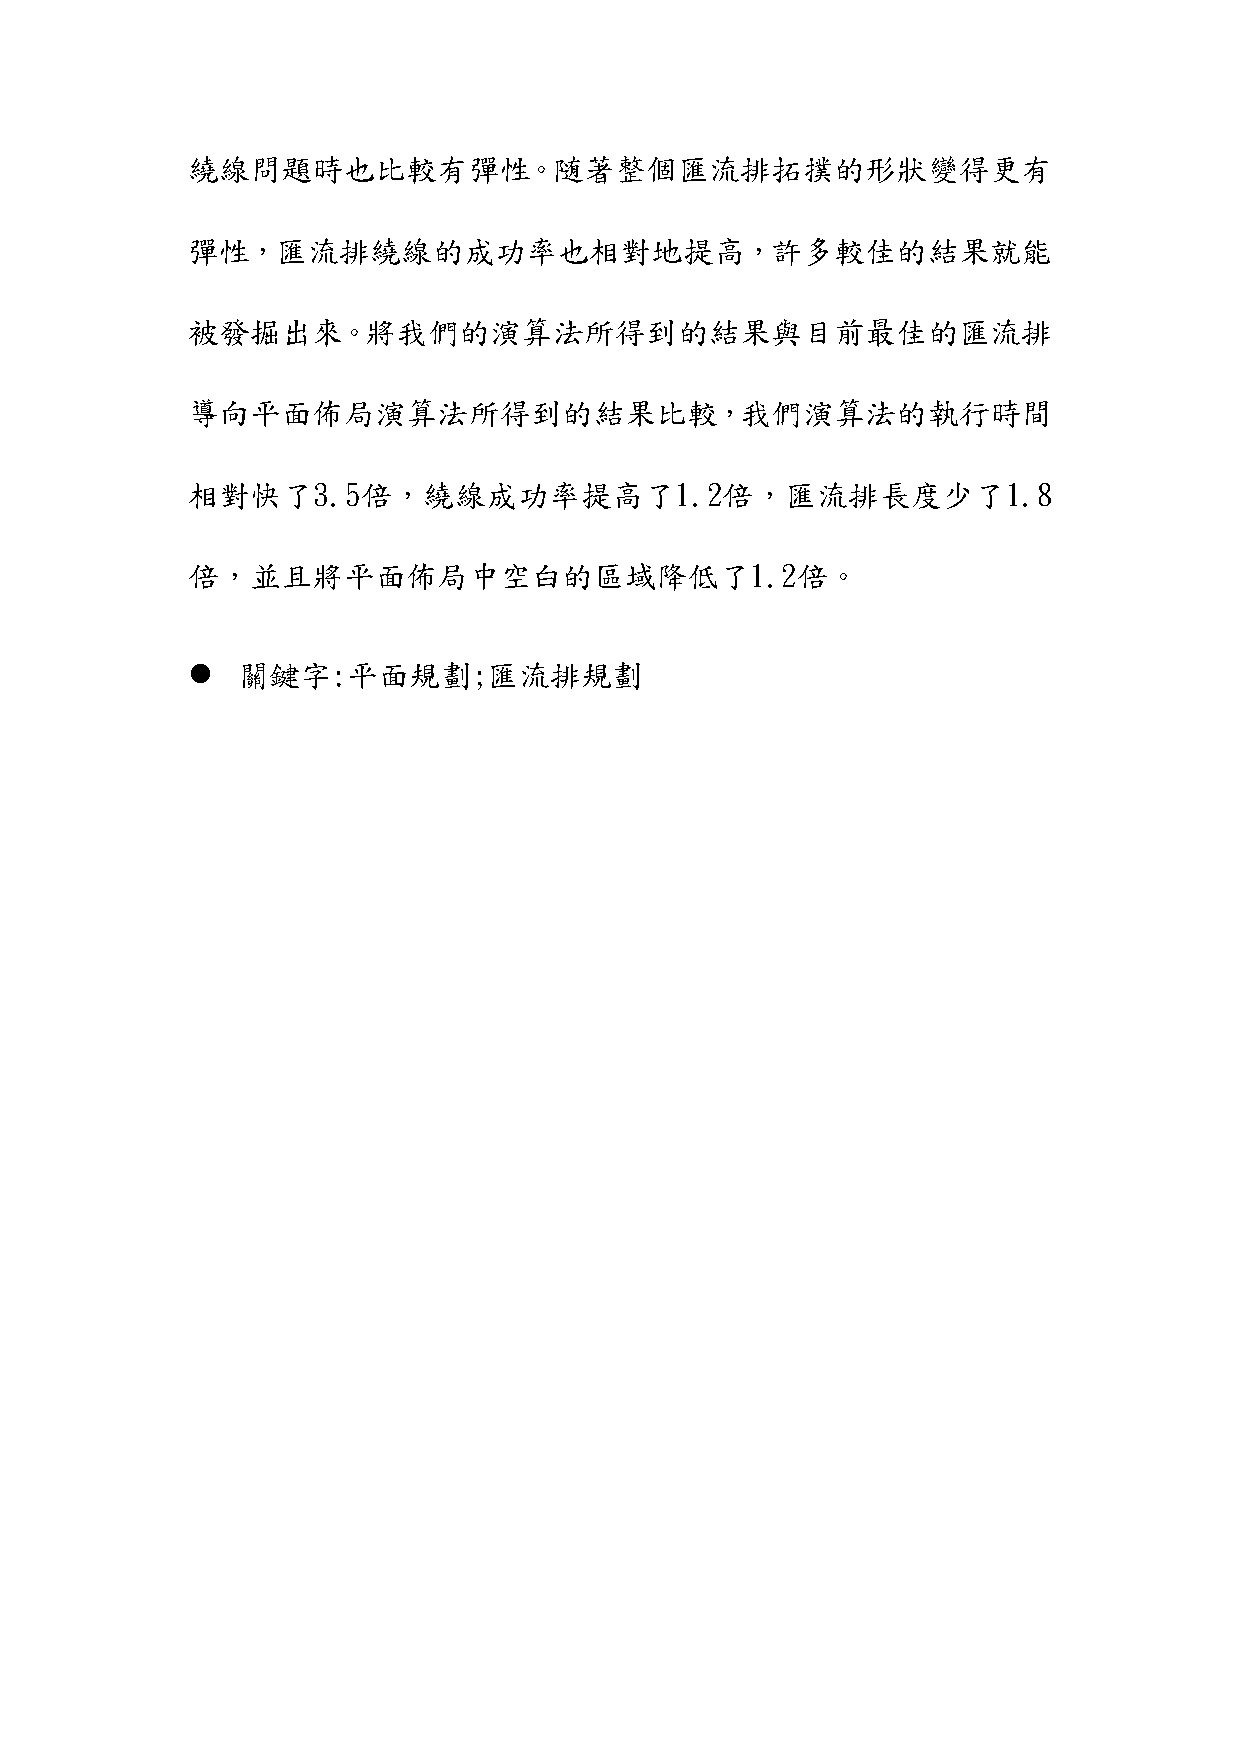
\includegraphics[]{./abstract/ChineseAbstract2.pdf}
\end{tabular}
\end{figure}
\newpage
\newpage



%
% Place your English abstract here. The abstract heading will be
% generated automatically.
% Note: do NOT use \begin{abstract} ... \end{abstract}
%
\begin{center}
\large \textbf{Bus-Pin-Aware Bus-Driven Floorplanning} \\[15mm]
\normalsize \textbf{Student: Po-Hsun Wu \hspace{5mm} Advisor: Dr. Tsung-Yi Ho\\[7mm]}
\normalsize \textbf{Department of Computer Science and\\
                    Information Engineering \\
                    National Cheng Kung University\\
                    Tainan, Taiwan, R.O.C.\\[7mm]}
\large \textbf{Abstract}
\end{center}
%%%%%%%%%%%%%%%%%%%%%%%%%%
\label{abs}
%%%%%%%%%%%%%%%%%%%%%%%%%%

\baselineskip=26pt


As the number of buses increase substantially in multi-core SoC
designs, the bus planning problem has become the dominant factor
in determining the performance and power consumption of SoC
designs. To cope with the bus planning problem, it is desirable to
consider this issue in early floorplanning stage. Recently,
bus-driven floorplanning problem has attracted much attention in
the literature. However, current algorithms adopt an
over-simplified formulation ignoring the position and
orientation of the bus pins, the chip performance may be deteriorated.
In this paper, we propose the bus-driven
floorplanning algorithm that fully considers the impacts of the bus
pins. By fully utilizing the position and orientation of the bus pins,
bus bendings are not restricted to occur at the modules on the bus,
then it has more flexibility during bus routing. With more
flexibility on the bus shape, the size of the solution
space is increased and a better bus-driven floorplanning solution
can be obtained. Compared with the bus-driven
floorplanner \cite{Ma08}, the experimental results show that our
algorithm performs better in runtime by 3.5$\times$, success rate
by 1.2$\times$, wirelength by 1.8$\times$, and reduced the
deadspace by 1.2$\times$.


\begin{itemize}
\item {\bf Keywords:} Floorplanning; Bus planning

\end{itemize}
               % English Abstract


% ------------------------------------------------

% 致謝 Acknowledgments
% ------------------------------------------------
\StartAcknowledgmentsChi
% ------------------------------------------------

在這邊寫你的感謝 (對父母, 老師, 同學, 朋友等的感謝).

% ------------------------------------------------
\EndAcknowledgments
% ------------------------------------------------

% ------------------------------------------------

\ifthenelse{\GetLangEnableChi = 1}
{
  % ------------------------------------------------
\StartAcknowledgmentsChi
% ------------------------------------------------

在這邊寫你的感謝 (對父母, 老師, 同學, 朋友等的感謝).

% ------------------------------------------------
\EndAcknowledgments
% ------------------------------------------------

}{}

\ifthenelse{\GetLangEnableEng = 1}
{
  % ------------------------------------------------
\StartAcknowledgments{chapter:acknowledgments}
% ------------------------------------------------

Thanks someone you want here.

Ask Google\cite{website:google} if you need. (If you set some references file, you need to use at least one cite to make Latex work.)

% ------------------------------------------------
\EndAcknowledgments
% ------------------------------------------------

}{}

% ------------------------------------------------


% ------------------------------------------------

% 目錄 (內容, 圖表和圖片) Index of contents, tables and figures.
% 內容會自動產生 The indices will generate in automate.
%
% This file is part of ncku-thesis-templete.
%
% ncku-thesis-templete is distributed in the hope that it will be useful,
% you can redistribute it and/or modify
% it under the terms of the Attribution-NonCommercial-ShareAlike
% 4.0 International.
%
% You should have received a copy of the
% Attribution-NonCommercial-ShareAlike 4.0 International
% along with ncku-thesis-templete.
%
% If not, see <http://creativecommons.org/licenses/by-nc-sa/4.0/legalcode.txt>.
%

% 目錄 (內容, 圖表和圖片)
% Index of contents, tables and figures
\newpage

\phantomsection
%\addcontentsline{toc}{chapter}{Contents}
\tableofcontents

\phantomsection
%\addcontentsline{toc}{chapter}{Tables}
\listoftables

\phantomsection
%\addcontentsline{toc}{chapter}{Figures} 
\listoffigures



% ------------------------------------------------

% Introduction section
% ------------------------------------------------
\StartChapter{Introduction}{chapter:introduction}
% ------------------------------------------------

\StartSection{介紹}

這是國立成功大學碩博士用畢業論文的LaTex模板. 本模板是使用學校最新的畢業論文要求來設計(參考: 附錄 - 撰寫論文須知 P.\RefPage{appendix:thesis-spec}).

雖然本模板的目標是為了提供學生可以使用LaTex來寫畢業論文. 但是各系所有各自的格式, 所以做了一個表列出已知的系所情況(參考: 附錄 - 可使用的系所 P.\RefPage{appendix:acceptable-dept}), 故請在使用前先留意自己的系所有沒有格式要求. 如果沒有, 則本模板應該是可以用來使用; 否則要看系所上的格式, 是否跟本模板有相同的寫法.

本模板分以下幾個主要部份來進行教學:
\begin{enumerate}
  \item 本模板的架構設計
  \item 設定本模板的一些資料以轉成你的論文
  \item 介紹Latex和本模板所提供的語法
  \item 最後有一個chapter為"老師們的話"(Chap. \RefTo{chapter:words-from-teacher})寫了一些老師對論文的想法和意見, 以供同學們留意
\end{enumerate}
同學們只要閱讀完後, 把部份的檔案直接copy和修改內容, 應該很快就能上手本模板去寫自己的論文.

另外在附錄(appendix)附上了一些重要的學校的文件, 由於本模板很接近完善, 故直接使用本模板後可不需再閱過學校相關規定之文件, 所以該類文件置於此僅為備考用.

% ------------------------------------------------
%\newpage

\begin{description}
  \item[版權 License] \hfill
  \InsertImage
    [scale=0.8, align=center,
      caption={CC Attribution-NonCommercial-ShareAlike License},
      label={fig:appendix:by-nc}]
    {./example/introduction/pic/by-nc-sa.png}

    本著作(ncku-thesis-templete-latex\RefBib{web:this-project:github})採用創用 CC 姓名標示-非商業性-相同方式分享 4.0 授權條款.

    This work(ncku-thesis-templete-latex\RefBib{web:this-project:github}) is licensed under Creative Commons Attribution-NonCommercial-ShareAlike 4.0 International License.

  詳細請看'LICENSE'這檔案中的條款說明.

  \item[版本修改 ChangeLog] \hfill
    % ------------------------------------------------
\begin{description}
  \item[v1.3.0] 重大改版 (如果是使用升級方式, 請注意以下所修改的部份有沒有影響自身的版本)\hfill
    \begin{description}
      \item[其他] \hfill
        \begin{enumerate}
          \item 更新CONTRIBUTE中的名單和使用的稱號
        \end{enumerate}
    \end{description}

  \item[v1.2.8] 修正日期在英文書脊中, 會因月份文字的長度而影響位置不一樣的問題

  \item[v1.2.7] \hfill
    \begin{enumerate}
      \item 增加可放置論文題目的長度. 修正在封面和Oral文件的樣板中, 會在題目沒有很長情況下, 被強迫斷行. 長度控制交由同學自己斷行, 以造出比較漂亮題目
      \item 修正書脊中題目跟學位不是同一個高度的問題
      \item 修正英文Oral文件的樣板會出現頁碼的問題
    \end{enumerate}

  \item[v1.2.5] 修正在'Objective'和'Acknowledgments'的錯誤內容

  \item[v1.2.4] 增加英文封面可同時顯示中英文 (\href{https://github.com/wengan-li/ncku-thesis-templete-latex/issues/3}{Issue \#3})

  \item[v1.2.3] \hfill
    \begin{enumerate}
      \item 修正統一使用'Fig'去取代'Fig.', 因為當使用'Fig.'時會產生更大的空格
      \item 修正在'表格 Table'中的圖片位置
      \item 移除在'圖片 Image'的'多張'中舊API的說明文字
      \item 修正在'圖片 Image'中插入多張的圖片時, 不管是主圖或子圖片都推薦使用'align = center'來進行置中, 除非是為了特殊的原因
    \end{enumerate}

  \item[v1.2.2] 修正在'Induection'中的'ChangeLog'和'License'中一些奇怪多餘的空白

  \item[v1.2.1] 修正中文書脊文字位置錯誤問題

  \item[v1.2.0] \hfill
    \begin{enumerate}
      \item Appendix新增'常見問題Q\&A'
      \item 把'Induection'中的'ChangeLog'改使用為單一'.tex'檔去存放
      \item 增加字眼'共同指導'或'Co-advisor'在封面上 (\href{https://github.com/wengan-li/ncku-thesis-templete-latex/issues/2}{Issue \#2})
      \item 重新調整中文封面中的中英文名字2邊的中間空間的大小, 以防止中文名字有4個字時, 出現overlap的問題
    \end{enumerate}

  \item[v1.1.6] 刪除'Induection'和'README.md'中的'版本 Version'

  \item[v1.1.5] 修正每個Chapter的第一頁的頁碼位置跟其他頁面不同的問題 (\href{https://github.com/wengan-li/ncku-thesis-templete-latex/issues/1}{Issue \#1})

  \item[v1.1.4] 修正目錄自己沒有在目錄的Linking中出現

  \item[v1.1.3] 修正README.md中內容的位置錯誤

  \item[v1.1.2] \hfill
    \begin{enumerate}
      \item 重寫有關figure API的code, 增加和優化那些功能 (如增加align)
      \item 更新README.md的內容
      \item 增加ChangeLog
    \end{enumerate}

  \item[v1.1.1] \hfill
    \begin{enumerate}
      \item 把'Abstract'的中文版本是以'摘要'來顯示
      \item 修改和改良有關oral文件的一些path位置
    \end{enumerate}

  \item[v1.1.0] \hfill
    \begin{enumerate}
      \item 增加版權資料到一些核心檔案
      \item 修改和增加一些圖書館要求的內容
      \item 修改有關abstract的一些path位置
      \item 正式得到學校有關部門對這模板的接受
    \end{enumerate}

  \item[v1.0.1] 修改少量錯誤的內容和URL連接

  \item[<= v1.0.0] 正式完成版本
\end{description}

% ------------------------------------------------

\end{description}

% ------------------------------------------------
\EndChapter
% ------------------------------------------------


% Objective section
% ------------------------------------------------
\StartChapter{Objective}{chapter:objective}
% ------------------------------------------------

\StartSection{起因}

做這個模版的原因其實很簡單:

\begin{enumerate}
  \item
  {
    去投國外paper時, 對方可能會要求使用LaTeX, 所以未來要懂LaTeX是不意外的.
  } % End of \item{}

  \item
  {
    想拿LaTeX來寫畢業論文, 卻發現學校只提供Mircosoft Word模版, 但卻沒有提供LaTeX的, 所以證明本模版對學校是有存在價值的.
  } % End of \item{}

  \item
  {
    因為看到發現台灣科技大學\RefBib{web:latex:template:ntust}, 台灣大學\RefBib{web:latex:template:ntu}, 元智大學\RefBib{web:latex:yzu}都能找到LaTeX的模版, 連大陸那邊都有一些學校有在提供, 更不用說國外的學校.

    那些學校的畢業論文模版不只提供是Mircosoft Word版本(.doc), 是會連Latex(.tex)版本都有, 而我們學校卻沒有. 唯一我們學校在Google上找到的有提到的卻是數學系系網頁上的功能\RefBib{web:latex:ncku_math_introduction}和建在數學系上的一個討論區\RefBib{web:latex:ncku_math_forum}.
  } % End of \item{}

  \item
  {
    因為學校對Phd跟Master的畢業論文要求是同一個格式, 所以如果完成後對學校任何學生應該都有其好處.

    對大家都有多一個選擇來寫畢業論文, 而不是被限在使用Mircosoft Word來寫.
  } % End of \item{}

  \item
  {
    經過詢問我們資訊工程系(CSIE)的系上一些老師後, 意外發現原來某些實驗室其實已經有各自的版本存在, 但每個版本都有各自的優缺點, 例如:

    \begin{enumerate}

      \item
      {
        新的使用者或接手的人不容易修改或使用.
      } % End of \item{}

      \item
      {
        或是需要安裝的步驟十分麻煩 (e.g cwTeX\RefBib{web:latex:cwtex}).
      } % End of \item{}

      \item
      {
        另外有一些因為是只針對英文版本, 沒有考量在編寫或初稿時會有中英混雜的時候(同時因學校奇怪的要求, 例如英文內容的論文卻要寫中文論文名字等), 所以需要把整個論文分開成不同格式的檔案.
      } % End of \item{}
    \end{enumerate}
  } % End of \item{}
\end{enumerate}

% ------------------------------------------------

\StartSection{目標}
所以為了解決以上的問題, 這個模版針對了好幾點來處理:

\begin{enumerate}

  \item
  {
    把本模版做到連笨蛋都可以很快懂得使用(所謂的Books for Dummies), 所以只留下使用者要填寫的部份外, 其他都交由模版去負責.
  } % End of \item{}

  \item
  {
    希望做到使用者只讀這份模版, 就會懂得去修改和寫自己所需的內容(所謂的Self-contained. 但其實是不太可能的, 因為Latex的使用手冊就算寫成一本幾百頁的書, 都可以缺少很多東西), 所以會同時提供很基本使用Latex的方式, 和填寫本模版步驟.
  } % End of \item{}

  \item
  {
    希望一份模版, 能同時應用在中文或是英文版本, 只要修改內容和一些的設定.
  } % End of \item{}

  \item
  {
    把本模版open source, 讓以後任何的同學們都可以使用和修改, 以合適當時的需求.
  } % End of \item{}

\end{enumerate}

而選擇使用XeLaTex的原因, 是經過分析cwTeX, CJK和XeLaTex後. 發現cwTeX的寫法太糟, 要背多新一種語法, 而且安裝複雜\RefBib{web:latex:cwtex}; 而CJK有一定程度的設定才能在整個論文中自由使用, 感覺設定麻煩而不太能笨蛋化來用, 所以放棄選用; 故最後選用最簡單加一些包裝, 就可以簡單使用中英混合的XeLaTex.

% ------------------------------------------------

\StartSection{缺點}
但是同樣任何東西都會有缺點, 故本模版都不意外:

\begin{enumerate}

  \item
  {
    本模版是以台灣國立成功大學所最新訂下的畢業論文要求(參考: 附錄 - 撰寫論文須知 P.\RefPage{appendix:thesis-spec})來設計, 所以不一定能對非本校的人有用.
  } % End of \item{}

  \item
  {
    對沒有程式基礎, 只會用Mircosoft Word的人來講, 可能會在修改或使用上會十分吃力.
  } % End of \item{}

  \item
  {
    因為我針對某些使用者不用去接觸的部份, 進行了大量的包裝(Wrapping), 所以如果懂得Latex的人可能會覺得我破壞了Latex的語法. 但是本模版是針對笨蛋化和全自動, 我相信對不會的人來講, 才不管這問題 (如同一般理論派和應用派的差別, 在意的方向完全不一樣).
  } % End of \item{}

  \item
  {
    某些包裝出來的語法, 可能會在一些情況下會產生衝突而令Latex不接受, 這時候有2種做法:
    \begin{enumerate}
      \item
      {
        不使用某些寫法, 例如已知的\begin{verbatim}\InsertFigure\end{verbatim}沒法被包在Table, minipage或framebox中.
      } % End of \item{}

      \item
      {
        如真的要使用那些情況, 那只好自己真的不使用我的語法, 而直接去寫Latex原版的語法.
      } % End of \item{}
    \end{enumerate}
  } % End of \item{}
\end{enumerate}

% ------------------------------------------------

\StartSection{總結}

以上是個人對這份模版的一些想法和起源, 同時希望本模版能對你提供到一些幫助.

% ------------------------------------------------
\EndChapter
% ------------------------------------------------


% ------------------------------------------------
\StartChapter{LaTex編寫教學}
% ------------------------------------------------

% ------------------------------------------------
\StartSection{基本介紹 Introduction}{chapter:how-to:write:intro}
% ------------------------------------------------

這教學包含了原LaTex和本模版特有的語法的使用方式和例子. (真正完完整整的LaTex教學手冊可不只單單幾百頁的厚度, 所以減少大家的時間, 所以本模版教學只講一些幾乎大家100\%會需要使用的語法).

請注意原LaTex語法會以英文小寫來顯示(\verb|\aabbcc|); 而本模版特有的語法會以英文大小寫混合(\verb|\AaBbCc|, 第一個字必定以大寫來顯示), 由於這些特有語法\textbf{不是}原LaTex的語法, 所以不能直接應用在非本模版的LaTex檔案上.

抄襲就是學習的第一步 (如同我們小時候去抄襲父母走路一樣), 所以本模版有留下了一些範本 (在`./context'下)以方便大家開始第一步, 之後就要靠大家自己的努力和實作, 再加上自己的探索能力了.

%\newpage
有問題的話, 可以有以下的地方找尋答案 (請使用這順序):
\begin{enumerate}
  \item 請一步一步增加內容, 如發生錯誤, 就把剛剛新增的內容拿掉, 以找出錯誤的地方
  \item 直接研究在模版的LaTex寫法 (在 './example' 以下的所有檔案)
  \item 查問懂得LaTex的老師和同學
  \item 去LaTex的Wikibook \RefBib{web:latex:wikibooks}\\
        這邊有大量的例子, 但是這些例子都是獨立的, 所以潛在語法混合後的會發生沖突的可能性; 另外都十分推薦去讀 '大家來學LaTeX' \RefBib{web:latex:latex123}
  \item 請求Google老師
\end{enumerate}

另外, 如果覺得本教學還缺少了什麼說明, 請告知.

% ------------------------------------------------

% Section
\newpage% ------------------------------------------------
\StartSection{基本語法 Basic syntax}{chapter:how-to:write:basic}
% ------------------------------------------------

這邊會講解一些最基本的功能.

% ------------------------------------------------
% ------------------------------------------------
\StartSubSection{字體變化}

\begin{itemize}
  \item
  {
    正常

    這是文字 This is text
  } % End of \item{}

  \item
  {
    粗體

    寫法:
    \begin{framed}
    \verb|\textbf{這是文字 This is text}|
    \end{framed}

    效果: \textbf{這是文字 This is text}
  } % End of \item{}

  \item
  {
    斜体

    寫法:
    \begin{framed}
    \verb|\textit{這是文字 This is text}|
    \end{framed}

    效果: \textit{這是文字 This is text}\\
    (中文的斜体並不太明顯)
  } % End of \item{}
\end{itemize}
% ------------------------------------------------


% ------------------------------------------------
\newpage% ------------------------------------------------
\StartSubSection{清單 List Structures}

  日常的清單主要有3種:

\begin{itemize}
  \item
  {
    數字

    可以有2種寫法, 使用\verb|\item xxxx|來只寫一行, 或是用\verb|{...}|可把內容包起來.\\

    \begin{DescriptionFrame}
    \begin{verbatim}
      \begin{enumerate}
      \item Item1

      \item Item2

      \item
      {
        Item3

        Item3's context
      }

      \item
      {
        Item4

        Item4's context
      }
      \end{enumerate}
    \end{verbatim}
    \end{DescriptionFrame}

    效果:
    \begin{enumerate}
      \item Item1

      \item Item2

      \item
      {
        Item3

        Item3's context
      }

      \item
      {
        Item4

        Item4's context
      }
    \end{enumerate}
  } % End of \item{}

  \newpage
  \item
  {
    符號

    \begin{DescriptionFrame}
    \begin{verbatim}
      \begin{itemize}
      \item Item1

      \item Item2

      \item
      {
        Item3

        Item3's context
      }

      \item
      {
        Item4

        Item4's context
      }
      \end{itemize}
    \end{verbatim}
    \end{DescriptionFrame}

    效果:
    \begin{itemize}
      \item Item1

      \item Item2

      \item
      {
        Item3

        Item3's context
      }

      \item
      {
        Item4

        Item4's context
      }
    \end{itemize}
  } % End of \item{}

  \newpage
  \item
  {
    文字

    可以有2種寫法, 使用\verb|\item[xxxx] xxxx|來只寫一行,\\
    或是用\verb|\hfill \\|把內容放到第2行才開始.\\

    \begin{DescriptionFrame}
    \begin{verbatim}
      \begin{description}
      \item[Item1] Item1's context
      \item[Item2] Item2's context
      \item[Item3] \hfill \\
        Item3's context
      \end{description}
    \end{verbatim}
    \end{DescriptionFrame}

    效果:
    \begin{description}
      \item[Item1] Item1's context
      \item[Item2] Item2's context
      \item[Item3] \hfill \\
      Item3's context
    \end{description}
  } % End of \item{}

  \newpage
  \item
  {
    巢狀表單

    表單應該最多只會用到第4層, 但是其實當你需要用到第3層時, 這時候你應該考慮的不是怎使用表單, 而是要怎換另外一種寫法了.\\

    \begin{DescriptionFrame}
    \begin{verbatim}
      \begin{enumerate}
        \item
        {
          Level-1 Item 1
          \begin{enumerate}
            \item Nested Item 1

            \item
            {
              Level-2 Item 2

              \begin{enumerate}
              \item
              {
                Level-3 Item 1
                \begin{enumerate}
                  \item Level-4 Item 1
                  \item Level-4 Item 2
                \end{enumerate}
              }
              \item Level-3 Item 2
              \end{enumerate}
            }
          \end{enumerate}
        }
      \end{enumerate}

      \begin{itemize}
        \item
        {
          Level-1 Item 1

          \begin{itemize}
            \item
            {
              Level-2 Item 2
              \begin{itemize}
                \item Level-3 Item 1
                \item Level-3 Item 2
              \end{itemize}
            }
            \item Level-2 Item 2
          \end{itemize}
        }
      \end{itemize}
    \end{verbatim}
    \end{DescriptionFrame}

    效果:
    \begin{enumerate}
      \item
      {
        Level-1 Item 1
        \begin{enumerate}
          \item Nested Item 1

          \item
          {
            Level-2 Item 2

            \begin{enumerate}
              \item
              {
                Level-3 Item 1

                \begin{enumerate}
                  \item Level-4 Item 1
                  \item Level-4 Item 2
                \end{enumerate}
              }

              \item Level-3 Item 2
            \end{enumerate}
          }
        \end{enumerate}
      }
    \end{enumerate}

    \begin{itemize}
      \item
      {
        Level-1 Item 1

        \begin{itemize}
        \item
        {
          Level-2 Item 2

          \begin{itemize}
          \item Level-3 Item 1
          \item Level-3 Item 2
          \end{itemize}
        }

        \item Level-2 Item 2
        \end{itemize}
      }
    \end{itemize}
  } % End of \item{}
\end{itemize}
% ------------------------------------------------


% ------------------------------------------------
\newpage% ------------------------------------------------
\StartSubSection{標記 Label}
標記(Label)是指給某項東西(如圖, 表格, 段落, chapter等)一個用來記憶的名字, 主要用來在引用時可以用來指定它. 使用方式是:

  \begin{framed}
  \begin{verbatim}
    \label{ ... some text here for your label ...} % 設定Label

    e.g
    \label{fig:introduction:fig1} % 設定Label
    \RefTo{fig:introduction:fig1} % 引用Label
  \end{verbatim}
  \end{framed}

Label的名字是可以任何輸入的文字, 但是為了方便記憶, 會固定以一個名字起頭, 再以段落/章節的方式來分隔.

\noindent 在例子中'fig:introduction:fig1':\\
以'fig'起頭: 即是目標是一張圖像(figure).\\
以'introduction'為章節: 即是目標放在introduction這一章中.\\
最後'fig1': 這張圖像的名字為'fig1'.

同樣其他方便記憶的目標起頭例如: 'website', 'table', 'chapter', 'section', 'paper', etc.

\newpage
\StartSubSection{引用 Reference}
因為原本Latex的引用語法可以引用很多東西, 所以可能會混亂不知道自己在引用什麼, 故本模板提供幾個語法來取代那些語法. (但是如果你是懂得原Latex的寫法(\verb|\ref{}, \cite{}, etc.|), 都可以直接使用原本的寫法, 其實是同一個東西.)

  \begin{framed}
  \begin{verbatim}
    引用 公式(Equation)
    \RefEquation{...}   直接顯示章節和它的號碼, 如: X.X
    \RefEquationB{...}  顯示時多了'()', 如: (X.X)

    引用 參考資料(References)
    \RefBib{...}   顯示號碼, 會加上'[]', 如: [X]

    引用 頁碼
    \RefPage{...}  顯示目標的頁碼, 如: X

    引用 其他任何的東西: 如圖片, 表格,
          chapter, section, subsection, etc.
    \RefTo{...}
      顯示章節和它的號碼, 如: X.X
      所以要手動在引用部份加上 fig, table, chap等一些字眼
  \end{verbatim}
  \end{framed}

由於label寫在Latex中, 而產生出來的後的文件是看不到的, 所以沒法簡單講解來說明, 所以可以參考後面的一些章節, 其內容會有一些例子會方便理解.

例子:
\begin{itemize}
  \item 圖片 - 可參考P. \RefPage{fig:example:mi2:mfig}.

  \item 表格 - 可參考P. \RefPage{chapter:how-to:write:table:label-example}.

  \item 公式(Equation) - 可參考P. \RefPage{chapter:how-to:write:equation:label-example}.
\end{itemize}

% ------------------------------------------------


% ------------------------------------------------
\newpage% ------------------------------------------------
\StartSubSection{註解 Comment}{chapter:how-to:write:comment}
% ------------------------------------------------

編寫任何內容時, 都會有一些作輔助用的內容, 這些內容正常不一定是用來顯示給別人看, 而是給自己作一些記憶用的.\\

但是在Word中所寫的任何內容, 正常都是寫來公開的, 而一些個人後備輔助用的資料就會寫在另一個檔案中; 但在LaTex中可以一同把這些資料寫在同一個檔案中, 但可指定不顯示, 這些叫註解(Comment).

  \EmptyLine
\begin{DescriptionFrame}
  \begin{verbatim}
    單行註解 (在第一個字使用'%'即可)

    % 註解內容 1
    % 註解內容 2
    顯示內容 1
       ...
    顯示內容 2
       ...
    

    多行註解 (把一個範圍內的內容為註解)

    \begin{comment}
    % 註解內容 1
    % 註解內容 2
    \end{comment}
    顯示內容 1
       ...
    顯示內容 2
       ...
  \end{verbatim}
\end{DescriptionFrame}



% ------------------------------------------------
\newpage% ------------------------------------------------
\StartSubSection{引用別的LaTex檔}

正常在編寫Word時, 都會把所有內容寫在同一個.doc中 (當然你都可能原本就喜好分開檔案來寫), 但在LaTex中這行為就不常見, 當內容很巨量的時候就更不用講, 這本模版更是其一例子.

  \EmptyLine
  \begin{DescriptionFrame}
  \begin{verbatim}
    引用的方式
    \input{ ... 檔案位置 ... }

    如現在你的檔案為:
    thesis.tex (主檔案)
    a.tex
    b.tex

    那要引用a.tex和b.tex時
    在thesis.tex中要寫
    \input{./a.tex}
    \input{./b.tex}
  \end{verbatim}
  \end{DescriptionFrame}
  \EmptyLine

如果還是不明白的話, 可以參考`./example'中的引用方式.

% ------------------------------------------------


\newpage% ------------------------------------------------
\StartSection{章節 Chapter/Section}{chapter:how-to:write:chapter-section}
% ------------------------------------------------

編寫任何的文章, 都會使用不同的章節來把內容進行分區. 例如這模版預設的樣子為:
\begin{DescriptionFrame}
  \vspace{0.2cm}
  \centerline{\LARGE Chapter X}
  \vspace{0.3cm}
  \centerline{\LARGE 這是標題}

  \vspace{0.5cm}
  \mbox{\Large X.1 節標題}\\
  \mbox{\hspace{1.2cm}內容 ...}

  \vspace{0.3cm}
  \mbox{\large X.1.1 小節標題}\\
  \mbox{\hspace{1.2cm}內容 ...}

  \vspace{0.3cm}
  \mbox{\large 小小節標題}\\
  \mbox{\hspace{1.2cm}內容 ...}
\end{DescriptionFrame}

所以針對這些功能, 本模版提供:
\begin{DescriptionFrame}
  \begin{verbatim}
    主要章節
    Title: 標題 (必填)
    Label: 標簽 (選填)
    \StartChapter{ Title }{ Label }
    \EndChapter % 用來保證你的內容在這Chapter內

    節
    Title: 標題 (必填)
    Label: 標簽 (選填)
    \StartSection{ Title }{ Label }

    小節
    Title: 標題 (必填)
    Label: 標簽 (選填)
    \StartSubSection{ Title }{ Label }

    小小節
    Title: 標題 (必填)
    Label: 標簽 (選填)
    \StartSubSubSection{ Title }{ Label }
  \end{verbatim}
\end{DescriptionFrame}

所以針對剛剛的例子, 它的LaTex寫法為:\\

\begin{DescriptionFrame}
  \begin{verbatim}
    \StartChapter{這是標題}

    \StartSection{節標題}
    內容 ...

    \StartSubSection{小節標題}
    內容 ...

    \StartSubSubSection{小小節標題}
    內容 ...

    \EndChapter
  \end{verbatim}
\end{DescriptionFrame}


\newpage% ------------------------------------------------

\newpage
\StartSection{Figure使用透明度}

\vspace{2.0cm}

\InsertFigure
  [scale=0.5,
    caption={opacity使用預設}]
  {./example/abstract/pic/extended-abstract-2.jpg}

\InsertFigure
  [scale=0.5,
    caption={測試opacity=0.4},
    opacity=0.4]
  {./example/abstract/pic/extended-abstract-2.jpg}

\newpage

\EmptyLine
\vspace{7.0cm}

    \InsertFigures
    [caption={opacity使用預設}] %
    {
      {./example/how-to/write/figure/pic/CC-BY-NC.png}
    }%
    {
      {./example/how-to/write/figure/pic/CC-BY-NC-ND.png}
    }

\vspace{1.0cm}

    \InsertFigures
    [caption={測試opacity=0.4},
    opacity=0.4]
    {
      {./example/how-to/write/figure/pic/CC-BY-NC.png}
    }%
    {
      {./example/how-to/write/figure/pic/CC-BY-NC-ND.png}
    }

% ------------------------------------------------

\newpage% ------------------------------------------------
\StartSection{表格 Table}{chapter:how-to:write:table}
% ------------------------------------------------

表格(Table)在任何情況下都是一個常用的顯示方式, 所以如何設計它都會有大量的玩法. 在正常Mircosoft Word這種有畫面的情況下, 可以慢慢拉出一個比較適合自己的, 但是在Latex中這個過程會是十分的痛苦, 因為你沒法馬上知道修改後的畫面, 故要不斷測試才知道效果, 這樣會大大減低選用table的使用次數.\\

在一般任何的Latex教學上, 如何編寫一個table出來都會是其中一項, 了解任何一個部份的寫法, 位置, 設定等. 但是由於那些資料十分的巨量 (不同寫法有不同效果), 所以這絕對不是使用本模版的大家想知道的東西, 故本模版不使用過往的方式, 而且直接教大家怎樣使用現有的online tool去處理掉這個問題.\\

以下的說明都是針對LaTeX Table Generator\RefBib{web:latex:table-generator}來進行說明. LaTeX Table Generator (Fig \RefTo{fig:how-to:table:table-generator})的頁面非常明瞭和簡單, 只要有過Mircosoft Word中的table設計的經驗, 應該要上手這個東西絕對不會很難.

\InsertFigure
  [scale=0.30,
  caption={LaTeX Table Generator頁面},
  label={fig:how-to:table:table-generator}]
  {./example/how-to/write/table/pic/table-generator.png}

% ------------------------------------------------
\newpage
\StartSubSection{產生Latex}

  我們使用這工具就是要去產生Latex用在論文當中, 所以這一步比其他的知識更為重要. 記得使用以下的步驟:

  \begin{enumerate}
  \item
  {
    使用畫面來設計table.
    \InsertImage
      [align=center]
      {./example/how-to/write/table/pic/table-view.png}
  } % End of \item{}

  \item
  {
    按Generate去產生Latex.
    \InsertImage
      [align=center]
      {./example/how-to/write/table/pic/generate.png}
  } % End of \item{}

  \item
  {
    複製Latex放到論文的".tex"中.
    \InsertImage
      [align=center]
      {./example/how-to/write/table/pic/latex-code.png}
  } % End of \item{}

  \item
  {
    執行XeLaTeX去產生效果.
  } % End of \item{}
  \end{enumerate}

  第1$\sim$3步會在整個設計table中常常都會使用, 所以會熟能生巧的. 而有經驗的人都知道, 第1步是最需要時間, 而第2$\sim$4步不用幾分鐘就能做完了, 所以只要用心的話, 多漂亮的table都是能弄出來的.

% ------------------------------------------------
\newpage
\StartSubSection{功能}

要設計一個複雜的table就需要足夠的功能才能慢慢弄, 所以在這邊介紹一些算是非常有用的功能.

\StartSubSection{File}

  在"File"中有幾個很有用的功能.
  \InsertImage
    [align=center]
    {./example/how-to/write/table/pic/menu-file.png}

  \begin{enumerate}

  % ------------------------------------------------
  \item
  {
    Import CSV file

    你可以直接upload一個CSV format的檔案之後弄table的外觀.
    \InsertImage
      [scale=0.7, align=center]
      {./example/how-to/write/table/pic/csv.png}
  } % End of \item{}

  % ------------------------------------------------
  \newpage
  \item
  {
    Paste table data

    可以把Microsoft Excel的table直接做Copy \& Paste到這一邊來.
    \InsertImage
      [scale=0.45, align=center]
      {./example/how-to/write/table/pic/paste.png}

    或是可以直接輸入資料來建立, 但要注意的是它只能接受CSV的寫法, 即是每一筆資料都是以","來分隔. 所以如果使用Fig \RefTo{fig:csv:enter-example-data}的寫法的話:
    \InsertImage
      [scale=0.65, align=center,
        caption={Enter example data},
        label={fig:csv:enter-example-data}]
      {./example/how-to/write/table/pic/paste-data.png}

    會出現Fig \RefTo{fig:csv:result-example-data}的效果:
    \InsertImage
      [scale=0.65, align=center,
        caption={Result of example data},
        label={fig:csv:result-example-data}]
      {./example/how-to/write/table/pic/paste-data-result.png}

  } % End of \item{}

  % ------------------------------------------------
  \newpage
  \item
  {
    Save table

    這online tool有一個十分有用的功能就是能把所做的table save下來, 只要輸入名字後再按download就會得到一個".tgn"檔案.
    \InsertImage
      [scale=0.8, align=center]
      {./example/how-to/write/table/pic/save-table.png}

    \InsertImage
      [align=center]
      {./example/how-to/write/table/pic/save-tgn.png}

  } % End of \item{}

  % ------------------------------------------------
  \item
  {
    Load table

    在"Save table"中得到的".tgn"檔案就是使用這邊來重新讀取table.
    \InsertImage
      [scale=0.8, align=center]
      {./example/how-to/write/table/pic/load-table.png}
  } % End of \item{}
  \end{enumerate}

\newpage
\StartSubSection{Edit}

  在"Edit"中有2個常用的功能

  \InsertImage
    [align=center]
    {./example/how-to/write/table/pic/menu-edit.png}

  \begin{enumerate}

  \item
  {
    Undo / Repeat

    很基本的重做上一步/下一步所做過的行為, 故不用解釋什麼.
  } % End of \item{}

  \item
  {
    Autosave

    這功能十分有用, 因為這tool是網頁tool, 所以正常重開網頁時會令到資料不見. 所以如果有把"Autosave"開啟的話, 那table就算接了"F5"都不會不見. (預設上應該會自動有開啟)
    \InsertImage
      [align=center]
      {./example/how-to/write/table/pic/edit-autosave.png}
  } % End of \item{}

  \end{enumerate}

% ------------------------------------------------
\newpage
\StartSubSection{Table}

  \begin{enumerate}

  \item
  {
    Set size

    這是table最基本的功能, 在Mircosoft Word時要插入多大的table時, 都要設定table的大小, 這邊正是那一個功能.
    \InsertImage
      [align=center]
      {./example/how-to/write/table/pic/table-set-size.png}
  } % End of \item{}

  \item
  {
    Clear table

    如果想把弄出來的table重新清掉所有設定和資料, 就是使用這一個.
    \InsertImage
      [align=center]
      {./example/how-to/write/table/pic/table-clear-table.png}
  } % End of \item{}

  \end{enumerate}

% ------------------------------------------------
\newpage
\StartSubSection{Extra options}

  在下方的"Extra options"有幾個基本的功能
  \InsertImage
    [align=center, scale=0.5]
    {./example/how-to/write/table/pic/options.png}

\begin{enumerate}

  \item
  {
  Center table horizontally

  把整個table置中在頁面
  \InsertImage
    [align=center, scale=0.5]
    {./example/how-to/write/table/pic/options-table-center.png}

  } % End of \item{}

  %\newpage
  \label{chapter:how-to:write:table:label-example}
  \item
  {
  Caption above / below, Label

  把圖表的標題要放在上方還是下方

  \InsertFigures
    [perrow = 2,
      caption = {Option of caption}] %
    {
      [scale=0.4,
      caption={標題放在上方}]
      {./example/how-to/write/table/pic/caption/above.png}
    }%
    {
      [scale=0.4,
      caption={標題放在下方}]
      {./example/how-to/write/table/pic/caption/below.png}
    }

  {\bf 注意:} 由於它沒有位置去修改caption和label, 所以要手動把caption和label中的內容修改.
  } % End of \item{}
\end{enumerate}

% ------------------------------------------------
\newpage
\StartSubSection{Style}

  在右邊可以設定table的style.
  \InsertImage
    [align=center]
    {./example/how-to/write/table/pic/style/style.png}

   正常在書本, 科學文章(如論文)和新聞中, table都是用三線式的方式, 因為這種的table簡單明瞭. 主要特點為整個table只有三條橫線, 上下兩端的線條較粗, 中間一條較細, 一般不使用分隔號.

  Fig \RefTo{table:style:sample-1}是一個例子分別是使用Latex原版的顯示方式(Fig \RefTo{table:style:default-1})或是使用booktabs版的顯示方式(Fig \RefTo{table:style:booktabs-1}).

  \InsertFigures
    [perrow = 2,
      caption = {A sample between Latex style and Booktabs style},
      label={table:style:sample-1}] %
    {
      [scale=0.3,
      caption={Default style},
      label={table:style:default-1}]
      {./example/how-to/write/table/pic/style/default-1.png}
    }%
    {
      [scale=0.2,
      caption={Booktabs style},
      label={table:style:booktabs-1}]
      {./example/how-to/write/table/pic/style/booktabs-1.png}
    }

  %\newpage
  而Fig \RefTo{table:style:sample-2}是2個版本都加上垂直線時候的樣子.

  \InsertFigures
    [perrow = 2,
      caption = {Table with horizontal line},
      label={table:style:sample-2}] %
    {
      [scale=0.3,
      caption={Default style}]
      {./example/how-to/write/table/pic/style/default-2.png}
    }%
    {
      [scale=0.25,
      caption={Booktabs style}]
      {./example/how-to/write/table/pic/style/booktabs-2.png}
    }

  就會發現booktabs版的中間的橫線比較細.

  這些都是一些細節問題, 如果想做簡單明瞭一些, 可以採用三線式表格, 但不是說只要是表格就必須使用三線式.

% ------------------------------------------------
%\newpage
\StartSubSection{其他}

  \begin{enumerate}

  \item
  {
    功能

    其他功能都很好理解的, 只要嘗試過就會明白, 所以不再作詳細解釋.
  } % End of \item{}

  \item
  {
    圖片

    這tool沒法插入圖片, 所以有關圖片的部份要自己加在table中, 請參考P. \RefPage{table:how-to:write:figure:insert-figure-into-table}, 但是在table中的figure是不能加標題和label.
  } % End of \item{}

  \item
  {
    備註

    而在產生出來的Latex中, 可以看到這類的文字(Fig \RefTo{table:package:comment}). 在注解中所講的, 是指所產生出來的Latex需要使用一些Latex的工具, 但這些工具已被包在本模版中, 所以可以無視的.

    \InsertImage
      [scale=0.7, align=center,
        caption={Package meno},
        label={table:package:comment}]
      {./example/how-to/write/table/pic/table-comment.png}
  } % End of \item{}
  \end{enumerate}

% ------------------------------------------------
\newpage
\StartSubSection{使用斜線}

斜線在表格上的設計是非常普遍, 但正如這一章開始時提到, Latex在表格設計上不直覺, 有很多功能都要自行處理, 斜線這一功能正是其一. 在LaTeX Table Generator中是沒法弄出斜線的, 故需弄完表格後再修改內容. 以下的內容都是拿自斜線工具的文件 \RefBib{web:latex:diagbox-doc}, 只抽出一些重要內容.

  \EmptyLine
  \begin{fmpage}{\textwidth}
  \begin{verbatim}
  Options 斜線的設定 (使用','來分隔, 不分先後順序)
    width:  畫斜線的格子寬度 (選填, 推薦使用以cm/mm來設定)
    height: 畫斜線的格子高度 (選填, 推薦使用以cm/mm來設定)
    dir:   斜線的方向 (選填, 預設: NW)
      NW: 由左上向右下, NE: 由右上向左下
      SW: 由左下向右上, SE: 由右下向左上

  Content 表格在這格子中的內容文字 (可設2~3個)

  插入斜線
    \diagbox[Options]{Content}

  E.g
    \diagbox{A}{B}{C}

    \diagbox[dir=NW, width=1cm, height=1cm]{A}{B}
  \end{verbatim}
  \end{fmpage}
  \EmptyLine

  一個最基本的例子:
  \begin{verbatim}
    \begin{tabular}{|l|ccc|}
      \hline
      \diagbox{Time}{Day} & Mon & Tue & Wed \\
      \hline
      Morning & used & used & \\
      Afternoon & & used & used \\
      \hline
    \end{tabular}
  \end{verbatim}

  \begin{table}[H]
  \centering
  \begin{tabular}{|l|ccc|}
    \hline
    \diagbox{Time}{Day} & Mon & Tue & Wed \\
    \hline
    Morning & used & used & \\
    Afternoon & & used & used \\
    \hline
  \end{tabular}
  \end{table}

% ------------------------------------------------
\newpage

  如果是給3個的話:
  \begin{verbatim}
    \begin{tabular}{|l|ccc|}
    \hline
    \diagbox{Time}{Room}{Day} & Mon & Tue & Wed \\
    \hline
    Morning & used & used & \\
    Afternoon & & used & used \\
    \hline
    \end{tabular}
  \end{verbatim}

  \begin{table}[H]
  \centering
    \begin{tabular}{|l|ccc|}
    \hline
    \diagbox{Time}{Room}{Day} & Mon & Tue & Wed \\
    \hline
    Morning & used & used & \\
    Afternoon & & used & used \\
    \hline
    \end{tabular}
  \end{table}

  \EmptyLine

  % ------------------------------------------------
  如Column或Row標頭需要斷行的話都是可以:
  \begin{verbatim}
    \begin{tabular}{|c|}
    \hline
    \diagbox{Row\\header}{Col\\header} \\
    \hline
    \end{tabular}
  \end{verbatim}

  \begin{table}[H]
  \centering
    \begin{tabular}{|c|}
    \hline
    \diagbox{Row\\header}{Col\\header} \\
    \hline
    \end{tabular}
  \end{table}

% ------------------------------------------------
\newpage

  使用以上的設定和組合可以玩出比較複雜的應用.

  \begin{verbatim}
    \begin{tabular}{|l|c|c|r|}
      \hline
      \diagbox{Time}{Day} & Mon & Tue & Wed\\
      \hline
      Morning & used & used & used\\
      \hline
      Afternoon & & used & \diagbox[dir=SW]{A}{B} \\
      \hline
    \end{tabular}
  \end{verbatim}

  \begin{table}[H]
  \centering
    \begin{tabular}{|l|c|c|r|}
      \hline
      \diagbox{Time}{Day} & Mon & Tue & Wed\\
      \hline
      Morning & used & used & used\\
      \hline
      Afternoon & & used & \diagbox[dir=SW]{A}{B} \\
      \hline
    \end{tabular}
  \end{table}

% ------------------------------------------------
\newpage

最後就是斜線長度是跟隨表格中最寬的那個寬度, 故如果對寬度不滿意, 可自行調整\verb|\diagbox|的width.

  \begin{verbatim}
    \begin{tabular}{|c|} \hline
      \diagbox{A}{B} \\\hline
      Very long term \\\hline
    \end{tabular}
  \end{verbatim}

  \begin{table}[H]
  \centering
    \begin{tabular}{|c|} \hline
      \diagbox{A}{B} \\\hline
      Very long term \\\hline
    \end{tabular}
  \end{table}

  調整成:
  \begin{verbatim}
    \begin{tabular}{|c|} \hline
      \diagbox[width=3cm]{A}{B} \\\hline
      Very long term \\\hline
    \end{tabular}
  \end{verbatim}

  \begin{table}[H]
  \centering
    \begin{tabular}{|c|} \hline
      \diagbox[width=3cm]{A}{B} \\\hline
      Very long term \\\hline
    \end{tabular}
  \end{table}

% ------------------------------------------------
\newpage
\StartSubSection{模版提供的功能}

在畢業論文中, 表格的位置跟圖片一樣都是非常固定以中間為主, 而不一樣的東西主要是表格的標題位置和表格的設計, 同時為了幫同學們調整好表格的故使用斜線則必須自行在內容中進行修改位置, 大小和預設白色背景, 故本模版同時增加一個幫助你插入表格的功能.

  \EmptyLine
  \begin{fmpage}{\textwidth}
  \begin{verbatim}
  Content:   表格內容 (必填)
    只需要\begin{tabular} ... \end{tabular}這部份的內容

  Options 設定 (使用','來分隔, 不分先後順序)
    scale:   頁面的比例 (選填, 預設: 0.0)
    (0.0: 原大小; 1.0: 跟頁面一樣大;
     0.x: 以比例的大小; 個人推薦最大值為0.9, 因需保留小量左右的空白)
    caption: 標題 (選填)
    label:   標簽 (選填, 必須要配合caption使用, 否則無效)
    pos:   caption在表格的位置
      top為上方, bottom為下面 (選填, 預設: top)

  插入表格
  \InsertTable[Options]{Content}

  E.g
    \InsertTable
    [caption={這 是 標 題}]
      {
        \begin{tabular}{ ... }
        ...
        \end{tabular}
      }

    \InsertTable
      [scale=0.5,
        pos=bottom,
        caption={這 是 標 題},
        label={this:is:label}]
      {
        \begin{tabular}{ ... }
        ...
        \end{tabular}
      }
  \end{verbatim}
  \end{fmpage}

% ------------------------------------------------

  \newpage
  {\bf 效果:}
  \begin{enumerate}

% ------------------------------------------------

  \item
  {
    標題在表格上方.
    \begin{verbatim}
    \InsertTable
      [caption={標題在上方}]
      {
        \begin{tabular}{|c|c|c|}
        \hline
         & Col 1 & Col 2 \\ \hline
        Row 1 & Value 1-1 & Value 1-2 \\ \hline
        Row 2 & Value 2-1 & Value 2-2 \\ \hline
        \end{tabular}
      }
    \end{verbatim}

    \InsertTable
      [caption={標題在上方}]
      {
        \begin{tabular}{|c|c|c|}
        \hline
         & Col 1 & Col 2 \\ \hline
        Row 1 & Value 1-1 & Value 1-2 \\ \hline
        Row 2 & Value 2-1 & Value 2-2 \\ \hline
        \end{tabular}
      }
  } % End of \item{}

% ------------------------------------------------

  \newpage
  \item
  {
    標題在表格下面.
    \begin{verbatim}
    \InsertTable
      [caption={標題在下面},
        pos=bottom]
      {
        \begin{tabular}{|c|c|c|}
        \hline
         & Col 1 & Col 2 \\ \hline
        Row 1 & Value 1-1 & Value 1-2 \\ \hline
        Row 2 & Value 2-1 & Value 2-2 \\ \hline
        \end{tabular}
      }
    \end{verbatim}

    \InsertTable
      [caption={標題在下面},
        pos=bottom]
      {
        \begin{tabular}{|c|c|c|}
        \hline
         & Col 1 & Col 2 \\ \hline
        Row 1 & Value 1-1 & Value 1-2 \\ \hline
        Row 2 & Value 2-1 & Value 2-2 \\ \hline
        \end{tabular}
      }
  } % End of \item{}

% ------------------------------------------------

  \newpage
  \item
  {
    Scale是用來調整表格的大小, 一般來講都不需要使用到這設定, 只有在特殊情況, 例如表格內容過多影響到寬度. 不同在Mircosoft Word中, 在Latex中表格是會無視寬度是否超過頁面的, 故這就需要靠scale來調整.Table \RefTo{table:how-to-write:table-example1} 是一個寬度超過頁面的例子, 而Table \RefTo{table:how-to-write:table-example2} 是把寬度控制跟頁面一樣闊, 但這就會沒有左右的空白空間, 而Table \RefTo{table:how-to-write:table-example3} 則是保留了左右的空白空間 (個人推薦最大值為0.9).

  \InsertTable
    [caption={表格寬度超過頁面},
      label={table:how-to-write:table-example1}]
    {
      \begin{tabular}{|c|c|c|c|c|c|c|c|c|c|c|c|c|c|c|c|}
      \hline
       & Col 1 & Col 2 & Col 3 & Col 4 & Col 5 & Col 6 & Col 7 & Col 8 & Col 9 & Col 10 & Col 11 & Col 12 & Col 13 & Col 14 \\ \hline
      Row 1 & Value & Value & Value & Value & Value & Value & Value & Value & Value & Value & Value & Value & Value & Value \\ \hline
      Row 2 & Value & Value & Value & Value & Value & Value & Value & Value & Value & Value & Value & Value & Value & Value \\ \hline
      Row 3 & Value & Value & Value & Value & Value & Value & Value & Value & Value & Value & Value & Value & Value & Value \\ \hline
      Row 4 & Value & Value & Value & Value & Value & Value & Value & Value & Value & Value & Value & Value & Value & Value \\ \hline
      \end{tabular}
    }

  \InsertTable
    [scale=1.0,
      caption={表格寬度設定scale=1.0},
      label={table:how-to-write:table-example2}]
    {
      \begin{tabular}{|c|c|c|c|c|c|c|c|c|c|c|c|c|c|c|c|}
      \hline
       & Col 1 & Col 2 & Col 3 & Col 4 & Col 5 & Col 6 & Col 7 & Col 8 & Col 9 & Col 10 & Col 11 & Col 12 & Col 13 & Col 14 \\ \hline
      Row 1 & Value & Value & Value & Value & Value & Value & Value & Value & Value & Value & Value & Value & Value & Value \\ \hline
      Row 2 & Value & Value & Value & Value & Value & Value & Value & Value & Value & Value & Value & Value & Value & Value \\ \hline
      Row 3 & Value & Value & Value & Value & Value & Value & Value & Value & Value & Value & Value & Value & Value & Value \\ \hline
      Row 4 & Value & Value & Value & Value & Value & Value & Value & Value & Value & Value & Value & Value & Value & Value \\ \hline
      \end{tabular}
    }

  \InsertTable
    [scale=0.9,
      caption={表格寬度設定scale=0.9},
      label={table:how-to-write:table-example3}]
    {
      \begin{tabular}{|c|c|c|c|c|c|c|c|c|c|c|c|c|c|c|c|}
      \hline
       & Col 1 & Col 2 & Col 3 & Col 4 & Col 5 & Col 6 & Col 7 & Col 8 & Col 9 & Col 10 & Col 11 & Col 12 & Col 13 & Col 14 \\ \hline
      Row 1 & Value & Value & Value & Value & Value & Value & Value & Value & Value & Value & Value & Value & Value & Value \\ \hline
      Row 2 & Value & Value & Value & Value & Value & Value & Value & Value & Value & Value & Value & Value & Value & Value \\ \hline
      Row 3 & Value & Value & Value & Value & Value & Value & Value & Value & Value & Value & Value & Value & Value & Value \\ \hline
      Row 4 & Value & Value & Value & Value & Value & Value & Value & Value & Value & Value & Value & Value & Value & Value \\ \hline
      \end{tabular}
    }

雖然內容可以保留在頁面中, 但看得出內容的文字會變小, 故表格的內容不能放過多內容, 否則會縮得十分的小.
  } % End of \item{}

% ------------------------------------------------

  \newpage
  \item
  {
    相反, 如果表格內容較少, 卻使用scale的話則會造成放大的行為.
Table \RefTo{table:how-to-write:table-example4} 是一個內容較少的表格, 而Table \RefTo{table:how-to-write:table-example5} 則設定了scale=0.9.

  \InsertTable
    [caption={內容較少的表格},
      label={table:how-to-write:table-example4}]
    {
      \begin{tabular}{|c|c|c|c|c|}
      \hline
       & Col 1 & Col 2 & Col 3 & Col 4 \\ \hline
      Row 1 & Value 1-1 & Value 1-2 & Value 1-3 & Value 1-4 \\ \hline
      Row 2 & Value 2-1 & Value 2-2 & Value 2-3 & Value 2-4 \\ \hline
      Row 3 & Value 3-1 & Value 3-2 & Value 3-3 & Value 3-4 \\ \hline
      Row 4 & Value 4-1 & Value 4-2 & Value 4-3 & Value 4-4 \\ \hline
      \end{tabular}
    }

% ------------------------------------------------

  \InsertTable
    [scale=0.9,
      caption={內容較少的表格, 但設定了scale=0.9},
      label={table:how-to-write:table-example5}]
    {
      \begin{tabular}{|c|c|c|c|c|}
      \hline
       & Col 1 & Col 2 & Col 3 & Col 4 \\ \hline
      Row 1 & Value 1-1 & Value 1-2 & Value 1-3 & Value 1-4 \\ \hline
      Row 2 & Value 2-1 & Value 2-2 & Value 2-3 & Value 2-4 \\ \hline
      Row 3 & Value 3-1 & Value 3-2 & Value 3-3 & Value 3-4 \\ \hline
      Row 4 & Value 4-1 & Value 4-2 & Value 4-3 & Value 4-4 \\ \hline
      \end{tabular}
    }
  } % End of \item{}


% ------------------------------------------------

  \newpage
  \item
  {
    有時候在寫Pseudocode時會使用Pseudocode (Chap. \RefTo{chapter:how-to:write:pseudocode})外, 都可能會直接使用Table來顯示, 以下是使用Hello World為例子.

    \begin{verbatim}
      \InsertTable
        [caption={Hello World in C}]
        {
          \begin{tabular}{ll}
          \hline
          1. & \#include \textless stdio.h\textgreater \\
          2. &  \\
          3. & int main(void) \\
          4. & \{ \\
          5. & \ \ \ \ \ \ \ \ printf("hello, world"); \\
          6. & \} \\ \hline
          \end{tabular}
        }
    \end{verbatim}

  \InsertTable
    [caption={Hello World in C}]
    {
      \begin{tabular}{ll}
      \hline
      1. & \#include \textless stdio.h\textgreater \\
      2. &  \\
      3. & int main(void) \\
      4. & \{ \\
      5. & \ \ \ \ \ \ \ \ printf("hello, world"); \\
      6. & \} \\ \hline
      \end{tabular}
    }
  } % End of \item{}

相比Pseudocode的缺點是沒有自動算行數和Keyword沒有變粗體, 所有內容都由自己控制.

% ------------------------------------------------

  \end{enumerate}

% ------------------------------------------------
\EndChapter
% ------------------------------------------------

\newpage% ------------------------------------------------
\StartSection{公式 Equation}{chapter:how-to:write:equation}

% ------------------------------------------------
\StartSubSection{介紹}

公式(Equation)在都是一個常用的顯示方式, 雖然寫法都很固定, 但是內容可以十分豐富, 這產生大量的寫法. 而Latex本身就擁有豐富的有關equation功能, Mircosoft Word都不一定有這麼多功能; 而且有一點Mircosoft Word是做不到, 但Latex就很輕鬆的行為是: 你無法很簡單帶走你所寫的Equation, 拿去轉成圖片或是copy到另一個文件中.

但是在Latex中, Equation跟Table(Chap \RefTo{chapter:how-to:write:table})都是一樣沒法即時知道修改後的畫面, 而且都會出現在基本教學中. 故本模板同樣教大家使用現有的online tool去處理掉這個問題.

% ------------------------------------------------
%\newpage
\StartSubSection{使用方式}
Equation有2種使用方式:
  \begin{enumerate}
    \item
    {
      跟文字寫在一起

      只要寫在2個\verb| $ |的符號之間, 即是\verb| $ ... $ |, 就可以顯示在文字之中.

      \noindent 例如:\\
      $E = mc^2$, 要寫成:\\
      \verb|      $E = mc^2$|\\
      而畢氏定理$c^2 = a^2 + b^2$, 要寫成:\\
      \verb|      畢氏定理($c^2 = a^2 + b^2$)是一個用來計算三角形的公式.|
    } % End of \item{}

    \newpage
    \item
    {
      使用本模板提供的語法.

      本模板結合了一些工具, 弄了\verb|\EquationBegin和\EquationEnd|這個語法, 在這個語法中所有公式都可以:
      \begin{enumerate}
        \item
        {
          可以在長公式的時候進行強制斷行

          只要在公式中插入\verb|\\|就可以強制斷行.
          \begin{verbatim}
            \EquationBegin
              x = a + b + c + \\
              d + e + f + g
            \EquationEnd
          \end{verbatim}

          {\bf 效果:}
          \EquationBegin
            x = a + b + c + \\
            d + e + f + g
          \EquationEnd
        } % End of \item{}

        %\newpage
        \label{chapter:how-to:write:equation:label-example}
        \item
        {
          在強制斷行下, 可以進行對齊位置

          使用\verb|&|就可以把你要的位置對齊, 以第一個\verb|&|為準則.
          \begin{verbatim}
            \EquationBegin
              x = &a + b + c + \\
              &d + e + f + g + \\
              &h + i + j + k
            \EquationEnd
          \end{verbatim}

          {\bf 效果:}
          \EquationBegin
            x = &a + b + c + \\
            &d + e + f + g + \\
            &h + i + j + k
          \EquationEnd
        } % End of \item{}

        \newpage
        \item
        {
          可設定標籤(Label)

          跟使用\verb|$...$|不一樣的是, 使用這個語法後, 每一個equation都會自動得到一個caption, 只要在\verb|\EquationBegin|加上\verb|{}|就可以為這個公式設定一個label來引用它.

          \begin{verbatim}
            \EquationBegin{eq:example:eq1}
              E = mc^2
            \EquationEnd
          \end{verbatim}

          e.g:
          \EquationBegin{eq:example:eq1}E = mc^2\EquationEnd

          使用\verb|\RefEquation|來引用:
          \begin{verbatim}Equation \RefEquation{eq:example:eq1}
              是Albert Einstein所想出來的.\end{verbatim}
          {\bf 效果:} Equation \RefEquation{eq:example:eq1} 是由Albert Einstein所想出來的.\\

          使用\verb|\RefEquationB|來引用 (數字會以\verb|'(X.X)'|)包起來:
          \begin{verbatim}這一條\RefEquationB{eq:example:eq1}
              是有名的物質轉成能量的equation.\end{verbatim}
          {\bf 效果:} 這一條\RefEquationB{eq:example:eq1}是有名的物質轉成能量的equation.
        } % End of \item{}
      \end{enumerate}
    } % End of \item{}
  \end{enumerate}

% ------------------------------------------------
\newpage
\StartSubSection{工具}

HostMath所提供的editor (Fig. \RefTo{fig:how-to:equation:hostmath})\RefBib{web:latex:equation:hostmath}頁面簡單明瞭, 包含了所有Latex支持的語法和斷行, 而且可以即時顯示Latex語法和結果. 因為使用十分簡單, 所以本模板不作深入的介紹.

\InsertCenterImage
  [scale=0.31,
    caption={HostMath's latex equation editor},
    label={fig:how-to:equation:hostmath}]
    {./example/how-to/write/equation/pic/hostmath.png}

因為要修改內容, 但是每一個符號都有一個語法(而且顯示為藍色), 但是其實多到背不完, 所以根本不需要去記它們. 所以這個時候可以使用最簡單(笨蛋)的方式, 就是1對1來修改, 上面語法修改了什麼, 下面變了什麼, 那就代表那段語法代表什麼.

只要背3個重要的語法就能寫出你的equation:
  \begin{itemize}
    \item \verb|^|: 上標
    \item \verb|_|: 下標
    \item \verb|{ ... }|: 區域, 這一個區域的內容會放在同一個位置
  \end{itemize}

在Fig. \RefTo{fig:how-to:equation:hostmath}已經舉了4個例子供大家理解.
% ------------------------------------------------
\newpage
\StartSubSection{轉成圖片}
HostMath是用來寫你的Equation, 但是如果你是把那條Equation轉成圖片的話, 可使用CodeCogs所提供的這個Latex equation editor\RefBib{web:latex:equation:codecogs}.

這Editor (Fig. \RefTo{fig:how-to:equation:codecogs})的頁面比HostMath來講有點簡陋, 但是重點是它可以轉出無失真的圖片(如.pdf, .eps, .svg), 這些圖檔在學術界內用來放在論文中是非常常見, 所以是十分有用的.

\InsertCenterImage
  [scale=0.27,
    caption={CodeCogs's latex equation editor},
    label={fig:how-to:equation:codecogs}]
    {./example/how-to/write/equation/pic/codecogs.png}

雖然簡陋, 但是使用上很簡單, 只要把Equation填進去, 之後選擇要ouput成什麼的圖檔, 那中間就會出現Equation的圖片和可按download的位置"Click here to Download Equation". 那download後就可以使用插入圖片 (Chap \RefTo{chapter:how-to:write:image})的方式來插入用來當成論文的用圖片.


\newpage% ------------------------------------------------
\StartSection{術語 Nomenclature}{chapter:how-to:write:nomenclature}
% ------------------------------------------------

Nomenclature在定義一些在整份論文中所會用到的變數是很常用到的. 它的位置會出現在文章當中或是在Chapter 1之前. 它的設計沒有一個標準答案, 在不同的情況下可能有不同顯示方式, 但它基本上跟一張Table是沒差的. 而它在Latex中是使用一個package名為`nomencl'.\\

但經過研究了一下package `nomencl'或tabbing這些用來建Nomenclature的方式後, 發現`nomencl'在設計上反而會增加在產生論文時的步驟; 而tabbing要自行定義一個闊度才能弄得比較好看, 但同時內容卻出現沒法置中和設計上等一些問題. 故最後決定直接套用Table來讓同學更能自由的設計不同的Nomenclature table.\\

設計Nomenclature table需要2個知識或工具:\\
1) 設計一張Table, 這邊請參考P. \RefPage{chapter:how-to:write:table}.\\
2) 有關所需要用到的符號, 請參考Equation (P. \RefPage{chapter:how-to:write:equation})中所使用到的工具, Texmarker左邊的工具列, 或看這幾個網頁\RefBib{web:symbols:site1}\RefBib{web:symbols:site2}\RefBib{web:symbols:site3}, 應該已經足夠同學們寫出合適的符號.

% ------------------------------------------------
%\newpage
\StartSubSection{使用方式}

如果是指是在Chapter 1之前的一大張的Nomenclature table, 為Nomenclature Chapter. 
  \begin{verbatim}
  \StartNomChapter{ NAME }{ LABEL }
  \EndNomChapter
  \end{verbatim}
Nomenclature Chapter跟一般Chapter的使用方式是一樣的, 但差別在於不會出現`Chapter'這字眼. 而由於大家的Nomenclature Chapter name可能不一樣, 故跟Chapter一樣可設定自行的name.\\

而如果是在文章當中的Nomenclature table. 基本上就是使用同一個的`\verb|\InsertTable|', 但還可以使用`nomtitle'來設定標題. `nomtitle'跟`caption'的差別是, 使用`nomtitle'所顯示出來的標題是沒有`Table XX:'為開頭, 同樣都是使用`pos'來控制題目的位置.

  \EmptyLine
  \begin{DescriptionFrame}
  \begin{verbatim}
  Options 設定
    nomtitle:   Nomenclature 標題 (選填)
    ...

  E.g
    \InsertTable
    [nomtitle={這是Nomenclature Table的標題}]
      {
        ...
      }
  \end{verbatim}
  \end{DescriptionFrame}
  \EmptyLine

有關這個的用法可參考`example/nomenclature/nomenclature.tex'中的Nomenclature Chapter所demo的例子, 那2個例子只是最簡單的Nomenclature table設計, 應該足夠同學們去弄出合適自己的Nomenclature table的設計.


\newpage% ------------------------------------------------
\StartSection{文獻引用 Bibliography/Reference}{chapter:how-to:write:bib}
% ------------------------------------------------

\StartSubSection{介紹}

Reference對論文來講十分重要的東西, 所以如果你引用的paper數量不少, 那在整理上會有點麻煩, 所以世界上有不少東西來管理這部份的資料, 如用的Word的話會配合Endnote.

而本模版是使用Latex中的BibTex來管理, 你可以在'./content/references'找到3個'.bib'檔, 那正是你可以把你所引用的內容放在裡面.

Bib的分類滿多 (參考\RefBib{web:latex:bib_manage}), 但論文主要都是引用'book' (課本, 書籍等), 'misc' (網頁, 任何其他東西), 'inproceedings' (論文類)中的內容, 所以本模版提供的樣板檔案為'book.bib', 'misc.bib' 跟 'paper.bib'.

\StartSubSection{使用方式}

任何放置論文的出版社(如ACM, IEEE, DBLP等), 都會為了方便別人去引用, 都會提供一些資料以給放在論文中引用. Fig \RefTo{fig:write:bib:1} 是以ACM Digital Library例子, 簡單說明如何使用BibTex來管理.

\InsertFigure
  [caption={ACM Digital Library例子},
    label={fig:write:bib:1}, scale=0.5]
  {./example/how-to/write/bib/pic/1.png}

\InsertFigure
  [caption={BibTex的位置},
    label={fig:write:bib:2}, scale=0.4]
  {./example/how-to/write/bib/pic/2.png}

在畫面右方會看到'Export Formats'的位置, 會看到如fig \RefTo{fig:write:bib:2}中一個的BibTex的按鈕.

\InsertFigure
  [caption={BibTex資料},
    label={fig:write:bib:3}, scale=0.5]
  {./example/how-to/write/bib/pic/3.png}

按它後就會出現如fig \RefTo{fig:write:bib:3}這個畫面, 這個就是要填進Bib的資料, 所以把這個東西複製到Bib檔內.

\InsertFigure
  [caption={整理/使用BibTex},
    label={fig:write:bib:4}, scale=0.5]
  {./example/how-to/write/bib/pic/4.png}

但複製完後要改一個東西, 第一行是所謂的label部份(參考Chap \RefTo{chapter:how-to:write:label}), 所以要改成一個自己能記得的label以方便在內容中來引用.

%有什麼問題可以去問Google\cite{website:google}老師. (如果有設定references用的檔案, 即使用了ReferencesFiles, 那必須至少要存在一個cite才不會顯示錯誤.)

% ------------------------------------------------
\EndChapter
% ------------------------------------------------

\newpage% ------------------------------------------------
\StartSection{虛擬程式碼(Pseudocode)}{chapter:how-to:write:pseudocode}
% ------------------------------------------------

Pseudocode在資訊類的paper是很常見, 雖然這東西冷門, 但是有它的存在意義.

而由於真的要寫Pseudocode的人, 理論上都100\%會寫程式, 所以有關這邊會直接使用例子(基本的function, if-elseif-else, while, return, switch-case)來說明, 靠例子應該就能寫出你所要的Pseudocode.

唯一注意的是需要使用:\\
'\verb|\Statex|'來斷一行空行\\
'\verb|\State|'來斷一行以寫新code在後面

% ------------------------------------------------

\newpage
\begin{algorithm}
  \caption{My algorithm (function A)}
  \label{algo:functionA}

  \begin{algorithmic}[1]
    \Function{function\_name\_a}{arg1, arg2}
      \If{conditionA}
        \State ...
      \ElsIf{conditionB}
        \State ...
      \Else
        \State ...
      \EndIf
      \Statex
      \If{condition1}
        \State ...
      \Else
        \If{condition2}
          \State ...
        \Else
          \State ...
        \EndIf
      \EndIf
      \Statex
      \For{condition}
        \State ...
      \EndFor
    \EndFunction
  \end{algorithmic}
\end{algorithm}

\newpage
針對function A (Algorithm \RefTo{algo:functionA}), 它的Latex寫法為:
    \EmptyLine
\begin{fmpage}{\textwidth}
  \begin{verbatim}
\begin{algorithm}
  \caption{My algorithm (function A)}
  \label{algo:functionA}

  \begin{algorithmic}[1]
    \Function{function\_name\_a}{arg1, arg2}
      \If{conditionA}
        \State ...
      \ElsIf{conditionB}
        \State ...
      \Else
        \State ...
      \EndIf
      \Statex
      \If{condition1}
        \State ...
      \Else
        \If{condition2}
          \State ...
        \Else
          \State ...
        \EndIf
      \EndIf
      \Statex
      \For{condition}
        \State ...
      \EndFor
    \EndFunction
  \end{algorithmic}
\end{algorithm}
  \end{verbatim}
\end{fmpage}

% ------------------------------------------------

\newpage
\begin{algorithm}
  \caption{My algorithm (function B)}
  \label{algo:functionB}

  \begin{algorithmic}[1]
    \Function{functionNameB}{}
      \State ...
      \State Some code here
      \State ...
      \Statex
      \While{condition3}
        \State ...
      \EndWhile
      \Statex
      \Repeat
        \State ...
      \Until{condition3}
      \Statex
      \Switch{condition4}
        \Case{condition5} ... \Break \EndCase
        \Statex
        \Case{condition6}
          \State ...
          \State \Break
        \EndCase
        \Statex
        \Default
          \State ...
        \EndDefault
      \EndSwitch

      \Statex\State \Return retValue
    \EndFunction
  \end{algorithmic}
\end{algorithm}

\newpage
針對function B (Algorithm \RefTo{algo:functionB}), 它的Latex寫法為:
    \EmptyLine
\begin{fmpage}{\textwidth}
  \begin{verbatim}
\begin{algorithm}
  \caption{My algorithm (function B)}
  \label{algo:functionB}

  \begin{algorithmic}[1]
    \Function{functionNameB}{}
      \State ...
      \State Some code here
      \State ...
      \Statex
      \While{condition3}
        \State ...
      \EndWhile
      \Statex
      \Repeat
        \State ...
      \Until{condition3}
      \Statex
      \Switch{condition4}
        \Case{condition5} ... \Break \EndCase
        \Statex
        \Case{condition6}
          \State ...
          \State \Break
        \EndCase
        \Statex
        \Default
          \State ...
        \EndDefault
      \EndSwitch

      \Statex\State \Return retValue
    \EndFunction
  \end{algorithmic}
\end{algorithm}
  \end{verbatim}
\end{fmpage}


% ------------------------------------------------
\EndChapter
% ------------------------------------------------


% ------------------------------------------------
\StartChapter{老師們的話 Words from teachers}{chapter:words-from-teacher}
% ------------------------------------------------

\section{介紹}

這部份的內容節錄於我跟系上老師的一些對話, 和上課所聽得出的結論和想法而整理出來的, 所以某些地方會帶有我們濃郁的資工系味道. 另外如果有任何的老師 (不論本系外系)可以提供一些意見或想法的話, 我會十分感謝的.

% ------------------------------------------------
\section{想法}

\begin{enumerate}
  \item
  {
    有用才算創新, 要站在使用者的角度去想
  } % End of \item{}

  \item
  {
    技術$\neq$研究, 是研究才有系統跟技術
  } % End of \item{}

  \item
  {
    研究
    \begin{itemize}
      \item
      {
        就是去想問題, 以不同的角度去想東西跟解決的方法
      } % End of \item{}

      \item
      {
        十分重要的是, 為什麼要這樣做, 這跟別人有什麼差別, 而且這樣做好處是什麼
      } % End of \item{}

      \item
      {
        '工程科系'是以多答案去解決一個問題, 而'理科'是提出一個標準的答案
      } % End of \item{}

      \item
      {
        不要相信直覺, 要所有東西都要證據
      } % End of \item{}

      \item
      {
        找研究題目的方法
      } % End of \item{}

      \begin{enumerate}
        \item
        {
          針對傳統的問題, 用方法不一樣去處理它
        } % End of \item{}

        \item
        {
          把一個問題的原本假設, 環境和條件之類的進行變動, 以得到不同的結果
        } % End of \item{}
      \end{enumerate}
    \end{itemize}
  } % End of \item{}
\end{enumerate}

% ------------------------------------------------
\section{投影片/presentation}

\begin{enumerate}
  \item
  {
    口試用PPT
    \begin{itemize}
      \item
      {
        要有outline, 而且要講大約要用多少時間來講
      } % End of \item{}

      \item
      {
        每個chapter都有一個頁面用來做分頁, 以讓口試委員知道聽到哪一個部份了
      } % End of \item{}

      \item
      {
        需要一些backup slide; 例如只講5張而已, 但backup用50張; 內容主要是一些data的來源, 和名詞解釋等
      } % End of \item{}
    \end{itemize}
  } % End of \item{}

  \item
  {
      1分鐘的報告
    \begin{itemize}
      \item
      {
        用one slide
      } % End of \item{}

      \item
      {
        主要使用graph
      } % End of \item{}

      \item
      {
        1,2 句的text
      } % End of \item{}

      \item
      {
        Some data
      } % End of \item{}

      \item
      {
        要做得能吸引眼睛
      } % End of \item{}
    \end{itemize}
  } % End of \item{}

  \item
  {
    一般報告paper
    \begin{itemize}
      \item
      {
        報1張ppt的時間應該是只有1分鐘左右 (除非詳細的系統架構圖), 因為讀1個中文字大約0.3秒
      } % End of \item{}

      \item
      {
        總原則
        \begin{enumerate}
          \item
          {
            解決了\textbf{'什麼'}的問題, 一定要非常清楚, 簡潔有力的說明
          } % End of \item{}

          \item
          {
            多用圖, 文字要讀完才能理解, 但圖可以有一看就懂的效果
          } % End of \item{}
        \end{enumerate}
      } % End of \item{}

      \item
      {
        Introduction
        \begin{enumerate}
          \item
          {
            什麼環境
          } % End of \item{}

          \item
          {
            什麼應用而造成這個問題
          } % End of \item{}

          \item
          {
            Given什麼條件
          } % End of \item{}

          \item
          {
            Find什麼條件
          } % End of \item{}

          \item
          {
            在什麼狀態下
          } % End of \item{}

          \item
          {
            Idea of the solution\\
            把最基本的精神講出來就可以, 不需要講detail
          } % End of \item{}
        \end{enumerate}
      } % End of \item{}

      \item
      {
        Related Work
        \begin{enumerate}
          \item
          {
            講解相關的研究
          } % End of \item{}

          \item
          {
            在1x分鐘中的報告是不用講, 除非如果不講相關的研究, 接下去觀眾就會完全不懂, 這才需要去提到 (因為是非常相關)
          } % End of \item{}
        \end{enumerate}
      } % End of \item{}

      \item
      {
        演算法
        \begin{itemize}
          \item
          {
            No
            \begin{enumerate}
              \item
              {
                不要講變數
              } % End of \item{}

              \item
              {
                不要把整個演算法顯示出來一步步講
              } % End of \item{}

              \item
              {
                不要用pseudocode
              } % End of \item{}
            \end{enumerate}
          } % End of \item{}

          \item
          {
            Yes
            \begin{enumerate}
              \item
              {
                盡量使用圖片來講解演算法
              } % End of \item{}
            \end{enumerate}
          } % End of \item{}
        \end{itemize}
      } % End of \item{}

      \item
      {
        公式
        \begin{enumerate}
          \item
          {
            不用講detail\\
            $ P( Q_{ni} ) = \frac{ 2^{k} - 1}{ 2^{n} - 1} $\\
            右邊部份不用說明\\
            只要講一整個公式的用途是在算什麼就行了
          } % End of \item{}

          \item
          {
            $ REL = A + B + C $\\
            只要講$REL$在算什麼就行了\\
            (除非別人不懂在講要算什麼, 才要把A, B, C都講出來大約算什麼則行了)
          } % End of \item{}
        \end{enumerate}
      } % End of \item{}

      \item
      {
        Theorem定理
        \begin{enumerate}
          \item
          {
            Definition\\
            在以後會常常說明的觀念, 為了以後方便講解和使用, 則使用Definition.\\
            在1x分鐘的報告中, 如果不常用,則不用講Definition, 如需要或常常會使用才需要.\\
          } % End of \item{}

          \item
          {
            Lemma\\
            是Theorem分開用來簡單說明的一個東西
          } % End of \item{}

          \item
          {
            Theorem\\
            是Lemma集合出的一個理論
          } % End of \item{}

          \item
          {
            Corollary\\
            在Theorem的結果用另一種條件或什麼得出的另一結果
          } % End of \item{}

          \item
          {
            Proposition\\
            以上的看情況來決定要不要講, 如果是跟algorithm無線電的, 則不用講, 否則要講一點點.\\

            如果不講定理, 都能講懂algorithm, 那則不用講.\\
            而如果algorithm會使用到一個小小的定理, 即只要講定理的結果.
          } % End of \item{}

          \item
          {
            Proof\\
            在報告時是絕對不用講的
          } % End of \item{}
        \end{enumerate}
      } % End of \item{}

      \item
      {
        Performance\\
        除非作者沒有提供任何做實驗的數據, 否則正常情況下都要講解這部份的內容.\\
        (有一些研究方向或實驗室, 沒有要求對這部份作要求的話, 那是可以不用說明的)\\
         
        必須說明作者使用的dataset是什麼, 環境是什麼等一些基本資料.\\
         
        之後作者做了什麼實驗, 效果如何, 發現了什麼.\\
         
        但是注意的是要對內容進行選擇, 不必要100\%的實驗資料都要拿出來講解, 只要講解這演算法最核心的一些實驗(如系統架構)就可以了.
      } % End of \item{}

      \item
      {
        優缺點, 建議 (十分重要)\\
        優點其實作者就會大力的說明, 所以不難找到.\\
         
        但是更重要的是, 作者一般都不會點出這演算法的缺點, 所以必須要看懂缺點在哪, 有什麼建議, 有什麼可以改進的方法, 或是有什麼方法可以用來延伸.
      } % End of \item{}

      \item
      {
        總結
        \begin{enumerate}
          \item
          {
            愈快讓人明白整個paper的要點.
          } % End of \item{}

          \item
          {
            最好能用圖片來說明.
          } % End of \item{}

          \item
          {
            Top-Down manner\\
            先講整體的觀念, 後才一部份一部份的講內容
          } % End of \item{}
        \end{enumerate}
      } % End of \item{}
    \end{itemize}

    科技論文, 是一開始就把結果說出來; 而其他的作文, 則是使用'起、承、轉、合'的手法. 但這是對論文是不對的.
  } % End of \item{}
\end{enumerate}

% ------------------------------------------------
\section{投論文的目標}

\begin{enumerate}
  \item
  {
    學位論文不影響以後把內容用來投去什麼的地方, 例如可以把學位論文100\%把內容移到journal中. 所以最重要的要做是優先把學位論文寫的, 才考慮投去哪
  } % End of \item{}

  \item
  {
    找paper用來投的地方, 可以到 "系網->學生事務->碩博士->期刊,會議點數"
  } % End of \item{}

  \item
  {
    寫完才考慮投去哪裡, 才把資料修成那邊要的樣子
  } % End of \item{}
\end{enumerate}

% ------------------------------------------------
\section{實驗的比較對象}

\begin{enumerate}
  \item
  {
    千萬不能對不同架構, 規模不一樣的對象來進行比較
  } % End of \item{}

  \item
  {
    用電腦系統來講
    \begin{itemize}
      \item
      {
        Single server只能跟single server比較
      } % End of \item{}

      \item
      {
        Distributed system只能跟distributed system來比
      } % End of \item{}
    \end{itemize}
  } % End of \item{}
\end{enumerate}

% ------------------------------------------------
\section{Related work}

只要有提到的對象, 就要去跟它比較; 不能比的就要去講差別; 有paper的就要去實作別人的部份功能

% ------------------------------------------------
\section{References}

\begin{enumerate}
  \item
  {
    要拿去哪投哪裡, 就起碼最少要引用一篇那邊的paper, 否則對方一般都不太想去看 (利益問題)
  } % End of \item{}

  \item
  {
    References所選的對象, 要根據這排名去選, 越高越有說服力:
    \begin{itemize}
      \item
      {
        Paper / book\\
        Paper所提出的東西一定會做過實驗或計算, 所以有一定的正確性. 但更新速度快, 所以會有很大量的.\\
        Book是經過好多年才會把一些正確的知識整合起來, 所以速度較慢, 但是以當代來講是最正確.
      } % End of \item{}

      \item
      {
        Tech report / Datasheet\\
        Tech report是一些人對某種東西去做研究或實驗, 所以他們會先把那個東西進行分析和理解, 故所寫出來的東西都經過他們的分析和研究, 雖然沒有paper那種程度的說服力, 但還是可以被人用來學習和引用的.\\
        Datasheet是一個系統或library的開發者所寫下來的, 因為他們是最懂得那東西, 所以使用他們的資料是可以被接受的.
      } % End of \item{}

      \item
      {
        Article\\
        Article是某些或某人去對一個主題去做, 所以所寫所說都是他們的立場或想法, 不一定100\%是正確; 但這些Article都是在反映人們對某主題的分析或理解, 所以可以代表以當代來講, 人們在意的部份是什麼.
      } % End of \item{}

      \item
      {
        URL / Website\\
        URL是最不應該當成References來使用, URL出現只能當符合以下情況:
        \begin{itemize}
          \item
          {
            URL所指向的是系統, tools, library的官方網站
          } % End of \item{}

          \item
          {
            URL所指向的是有關所使用的系統, tools, library的Datasheet
          } % End of \item{}

          \item
          {
            URL所指向的是Related work中要比較的對象它相關的資料會使用在這篇論文中, 如source code.
          } % End of \item{}
        \end{itemize}

        否則的話, 千萬不要放, 因為越多的URL, 說服力會越低.\\
 
        另外都千萬不要使用Wikipedia當成References, 雖然Wikipedia是知識解說的地方, 但Wikipedia正因為太普遍, 所以完全沒有任何特殊的說服力; 如同介紹人們去做search網頁時, 可以使用google, yahoo是同一個道理.
      } % End of \item{}
    \end{itemize}
  } % End of \item{}
\end{enumerate}

% ------------------------------------------------
\section{圖上的文字 / 表格}

除非特殊要求, 否則不能比正常的文字小 (必須 $ >= $ 10 pt), 要令人感覺每一個文字都是一樣大的, 要讓讀者可以一口氣看, 而不用做放大放小的行為.

% ------------------------------------------------
\section{寫作技術}

每一個新section的開頭段落, 不能以'所以', 'so'等文字, 而是必須要再用一些文字當起點, 如'前一章提到xxxxxx'.

% ------------------------------------------------
\section{內容}

\begin{enumerate}
  \item
  {
    Paper必須要做到self-contained, 要把用到的其他知識時, 必須要有example以解釋這thesis在說什麼
  } % End of \item{}

  \item
  {
    不能使用了別的東西, 而完全沒解釋是什麼意思, 要讀者去查References的資料去理解這thesis在做什麼
  } % End of \item{}
\end{enumerate}

% ------------------------------------------------
\section{公式}

\begin{enumerate}
  \item
  {
    避免重複做用\\
    $
      \begin{array}{ll}
            P(X) = \ldots & (A)\\
            P(X) = \ldots & (B)
      \end{array}
    $\\
    但2個$ P(X) $都代表不同的意思
  } % End of \item{}

  \item
  {
    大小寫不能一起用\\
    如 $ rel (a) $, $ REL(a) $, 但是不同意思
  } % End of \item{}

  \item
  {
    Subscript/superscript\\
    上下標是用來區分用的\\
    如$ w_{1} $, $ w_{2} $, $ w_{3} $ $ \ldots $.\\

    但不需要的話, 就不要加這個東西, 如:\\
    $
      \left\{
        \begin{array}{ll}
          r_{1}(a) & = \ldots\\
          r_{2}(a) & = \ldots 
      	\end{array}
      \right.
    $\\
    但2個$ r(a) $代表同一個意思
  } % End of \item{}

  \item
  {
    名字不要太長\\
    如$ sim(a,b) $\\
    因為很像similarity (相似), 所以可以使用, 但沒有近像的字, 就不要用寫這樣
  } % End of \item{}

  \item
  {
    變數沒用就不要寫\\
    如$ pv(u,a) = 1 / distance $\\
    $U$和$a$都是沒意義, 所以可以去掉
  } % End of \item{}
\end{enumerate}

% ------------------------------------------------
\EndChapter
% ------------------------------------------------


% Related Work section
%% ------------------------------------------------
% Page start
% ------------------------------------------------
\chapter{Related Work}
\label{chapter:related-work}

\baselineskip=26pt
\thispagestyle{empty}
% ------------------------------------------------

% Query Language section
\subsection{Query Language}

There are many non-relational database can use the SQL-like query language to query the database, such as Apache Hive of Hadoop, Cassandra Query Language (CQL), N1QL of Couchbase, ArangoDB Query Language (AQL), Hypertable Query Language (HQL), Cypher in Neo4j, etc.\\

Alought they may useful to its own database, but all of them have a basic common problem --- total un-compatible with standard SQL. This problem is the main reason that causing a huge gap between the relational and non-relational database, which makes many application can't easy swap the database to seek for the benefit of distributed database.

% CQEngine section
\minisec{- CQEngine \cite{web:cqengine:official} -}
\medskip
CQEngine (Collection Query Engine) is a Non-relational database indexing and query engine, for retrieving objects matching SQL-like queries from Java collections, with ultra-low latency. 它提供多種indexing的功能, 有Hash, Unique, Compound, Navigable, RadixTree, ReversedRadixTree, InvertedRadixTree, SuffixTree, StandingQuery, Fallback.

\begin{figure}[h]
\centering
%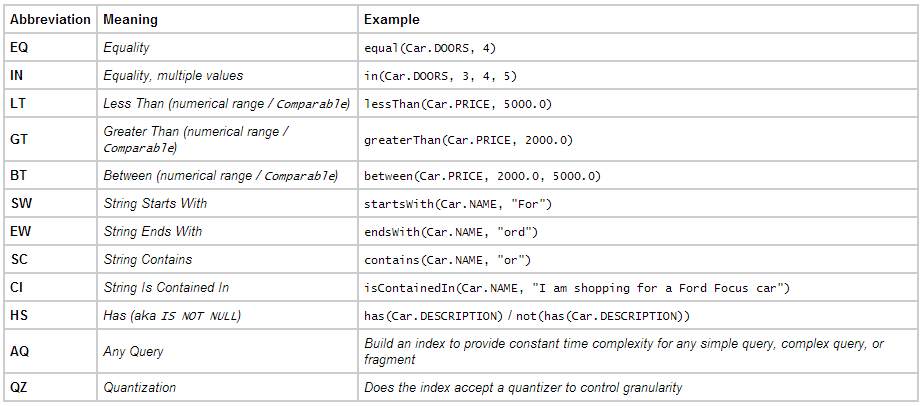
\includegraphics[scale=0.65]{./related-work/pic/CQEngine/CQEngine_index_1.png}
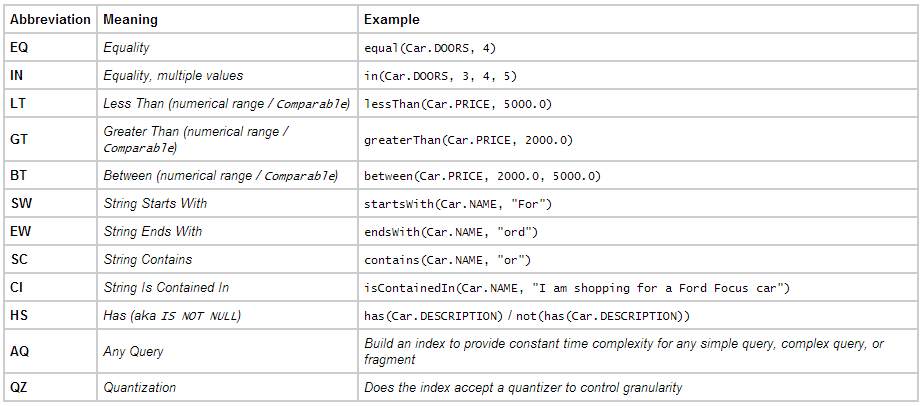
\includegraphics[width=0.8\textwidth]{./related-work/pic/CQEngine/CQEngine_index_1.png}
\caption{Legend for the feature matrix.}
\label{fig:related-work:legend_feature_matrix}
\end{figure}

\begin{figure}[h]
\centering
%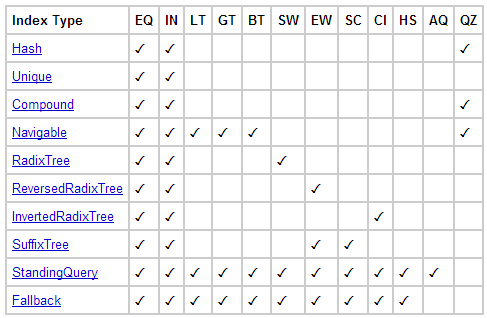
\includegraphics[scale=0.8]{./related-work/pic/CQEngine/CQEngine_index_2.png}
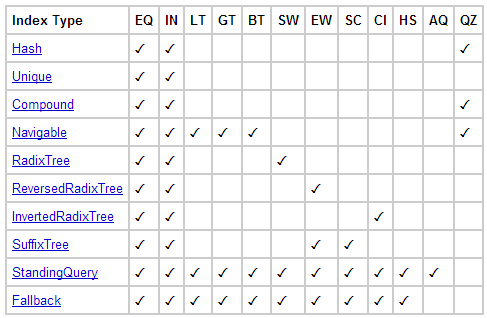
\includegraphics[width=0.8\textwidth]{./related-work/pic/CQEngine/CQEngine_index_2.png}
\caption{Index Feature Matrix.}
\label{fig:related-work:index_feature_matrix}
\end{figure}

User自己必須要定義自己的data是使用哪一定indexing的方式, 每一種indexing都只能做某一些特定的功能, 所以要先理解它們各自的特性.\\

雖然CQEngine是以indexing的想法來想提供key-value的application, 但它的使用方式卻不像現在的一些key-value的使用方式, 所以使用起來比較不friendly. From figure \ref{fig:related-work:example_useage}, we can see the simple of using CQEngine that the user need to define all the metadata.

\begin{figure}[h]
\centering
%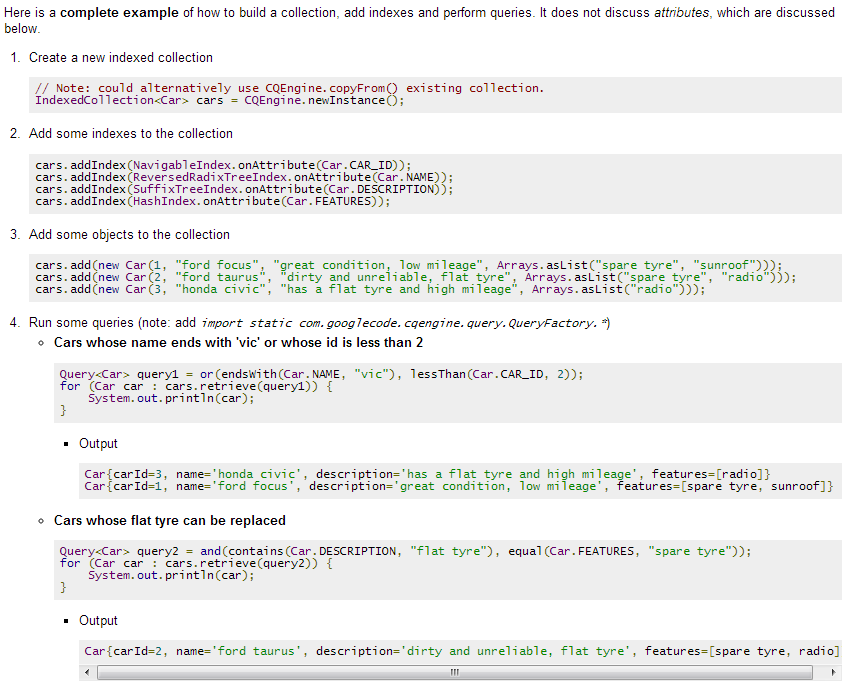
\includegraphics[scale=0.65]{./related-work/pic/CQEngine/CQEngine_index_3.png}
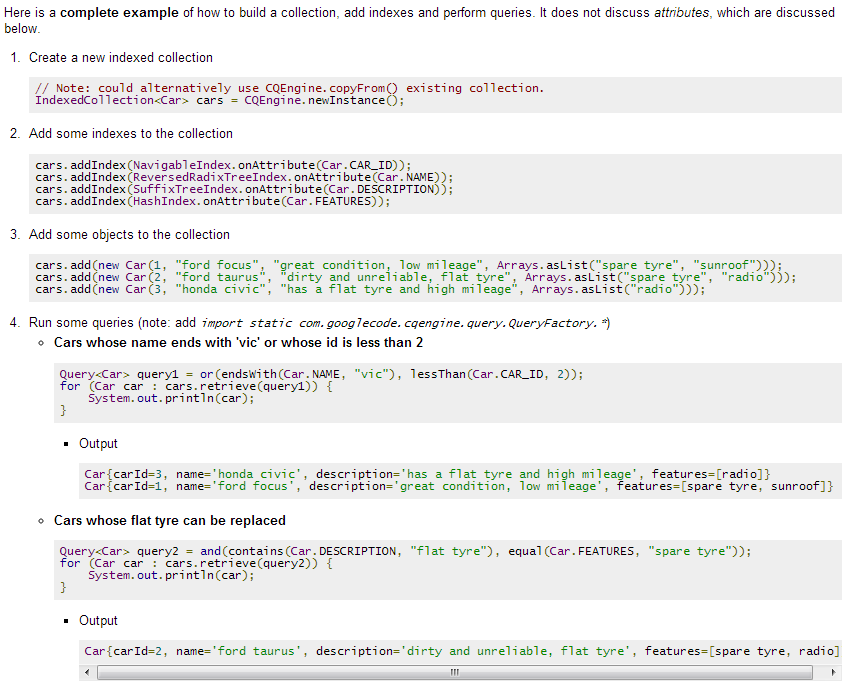
\includegraphics[width=0.9\textwidth]{./related-work/pic/CQEngine/CQEngine_index_3.png}
\caption{A complete example that how use the CQEngine.}
\label{fig:related-work:example_useage}
\end{figure}

CQEngine在想法上的確非常不錯, 但是CQEngine只有詳細說明query和indexing的效果和用法, 並沒有提及如何把data I/O到disk上, 所以可以假設它是in-memory database.

\clearpage

% Cassandra Query Language (CQL) section
\minisec{- Cassandra Query Language (CQL) \cite{web:cassandra:cql-tutorial} -}
\medskip
Apache Cassandra created by Facebook, Cassandra is a non-relational database distributed data store easily able to handle large amounts of writes and reads, a quality that has won favor with both high volume Internet services as well as with those firms executing big data-styled analysis.\\

\clearpage

% ArangoDB Query Language (AQL) section
\minisec{- ArangoDB Query Language (AQL) \cite{web:arangodb:aql-tutorial} -}
\medskip
AQL is a declarative query language similar to SQL and offers both simple and complex, nested queries. It can be used to retrieve data that is stored in ArangoDB.\\

\clearpage

% Storage engine section
\subsection{Storage engine}

So some research are maintain in relational database and do some improvement. Like \cite{paper:nodb,paper:spreadsheet-engine} are proposing swap the database engine to just use direct access the spreadsheet file (like CSV), which is very useful to some application and it can gain the benefit of distributed by using VFS (Virtual File System) mounting in Linux. This kind of design is suitable for common text and number data only, but not workable with the binary data like photos.

% NoDB section
\minisec{- NoDB \cite{paper:nodb} -}
\medskip
The authors in NoDB提出一個不用寫data到database, 就能以database的方式去query data的架構. 之後修改PostgreSQL來當成範例以證明NoDB是可以用在現在的database架構上, 在可用性和效率上得到好處.\\

他們提出了NoDB這個原因是去處理現在database技術中query反應的所需時間, 所以使用NoDB架構來減低讀取raw data的時間.\\

由於NoDB是設計成不用把data寫到database中, 所以它們的raw data是使用CSV files來當成data format, 之後database的任何行為都是在I/O CSV files. 而且data的indexing是使用dynamic allocation, 只有在處理query時才會產生出來, 而不是一直存在的, 所以不會需要有另外的indexing data在disk中.\\

這篇paper的確提出了一個新的做法去處理了一個到現在某些relational database系統中存在了40年的很基本的問題, 就是把所有data集中在一個地方. 問題就會出現在於如果要搬動database的話, 就要一整個database移動, 但如果database很大的話, this cost a huge of time. 但如果是多個CSV files, 在搬動時會十分方便, 而且可以控制mountpoint的方式去擴充database的空間, 這種擴充性也正是non-relational database在追求的其中一點.\\

而且因為data是CSV format, 但是不是任何data都是可以以CSV來處理, 例如non-structure和binary data, 這是data可能含有CSV用來分隔用的”comma”, 這會影響到讀取data的長度跟位置, 但是這篇paper中沒有討論相關的問題.

\clearpage

% Similar database section
\subsection{Similar database}

% Google F1 section
\minisec{- Google F1 \cite{paper:google-f1} -}
\medskip
To the best of our knowledge, Google F1 is the only one that can handle both kind of query (NoSQL and SQL) with fully functional in the current days.\\

Start from the Megastore (In chapter 3.2 of \cite{paper:google-megastore}), then up to the Spanner (At the introduction and chaper 2.3 of \cite{paper:google-spanner-1}) and the current F1 (Chapter 7 to 8 in \cite{paper:google-f1} or \cite{paper:google-f1-ad-business}). There is always mentioned about the SQL in the data model with the Protocol Buffer \cite{web:google:protocol-buffers}, this prove that even the database can be distrusted but still need a fully functional relational query interface to query the data which can't easy retrieve in a nomral \textit{get()} operation of non-relational database.\\

Google F1 is one of the database that can handle both kind of query (NoSQL and SQL) with fully functional in the current days. Start from the Megastore \cite{paper:google-megastore}, then up to the Spanner \cite{paper:google-spanner-1} and the current F1 \cite{paper:google-f1,paper:google-f1-ad-business} were always mentioned about the SQL in their data model.

% Conclusion section
\subsection{Conclusion}

This prove that even the database can be distrusted but still need a fully functional relational query interface to query the data which can't easy retrieve in a single \textit{get()} operation of non-relational database.

\clearpage

% ------------------------------------------------
% End of page
% ------------------------------------------------


% Algorithm  section
%% ------------------------------------------------
% Page start
% ------------------------------------------------
\chapter{Algorithm}
\label{chapter:algorithm}

\baselineskip=26pt
\thispagestyle{empty}
% ------------------------------------------------

\subsection{Design}

\subsubsection{Li's Hash}

Li's Hash is an algorithm that combines the concept of n-gram indexing \cite{web:wiki:n-gram} (Figure \ref{fig:algorithm:n-gram}), JSON (JavaScript Object Notation) \cite{web:wiki:json} (Figure \ref{fig:algorithm:json_example}) and hash table \cite{web:wiki:hash-table}.\\

JSON to store data which is exactly as same as hash table, but only different of the value's data type, which is because of the mapping design. And the n-gram indexing normally only target the data in string.\\

\begin{figure}[h]
\centering
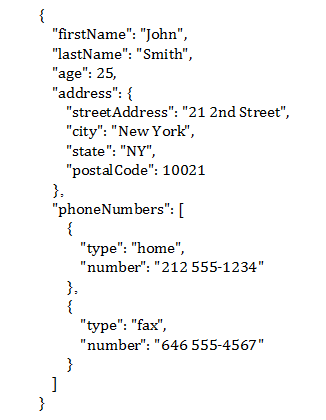
\includegraphics[scale=0.7]{./algorithm/pic/json_example_v1.png}
%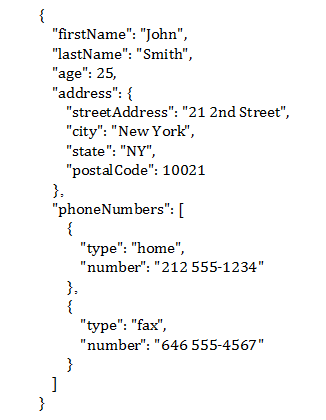
\includegraphics[width=0.4\textwidth]{./algorithm/pic/json_example_v1.png}
\caption{A example of JSON.}
\label{fig:algorithm:json_example}
\end{figure}

\begin{figure}[h]
\centering
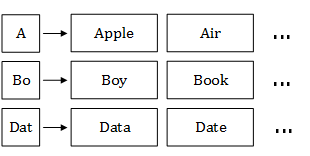
\includegraphics[scale=0.6]{./algorithm/pic/n-gram_v1.png}
%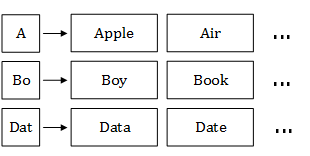
\includegraphics[width=0.4\textwidth]{./algorithm/pic/n-gram_v1.png}
\caption{A example of n-gram indexing.}
\label{fig:algorithm:n-gram}
\end{figure}

Combining all of them can form a special indexing structure which can store the data and query different data type of data, which can very useful for all kind of query and storage system design.\\

Also because Li's Hash is just an algorithm, so it can easily to suit for all kind of key-value stores, or just swap the back-end database that can use another without change any front-end code.\\

%\clearpage

% Data type section
\subsubsection{Data type}

Li's Hash try to fellow KISS (Keep It Simple \& Stupid) principle for user, so Li's Hash will only provide few basic data type to replace the general data type in SQL database \cite{web:mysql:data-types,web:mysql:data-types-store-requirements,web:sqlite:data-types-3,web:transact-sql:data-types}, to decrease the time that user need to understand all kind of data type before writing the code, and can be ignore the range of data type, to let them focus on their system design.\\

The provided data type are \textit{STRING}, \textit{INTEGER}, \textit{REAL}, \textit{BOOLEAN} and \textit{BLOB}. Table \ref{table:algorithm:database-layer:code-example} shows part of data type comparison between Li's Hash and relational database.

Table \ref{table:algorithm:data_type_description} is the description that the storage size and range about each data type.\\

\begin{table}[h]
\centering
\caption{Data type comparison}
\label{table:algorithm:database-layer:code-example}
\begin{tabular}{|c|c|}

\hline
\multicolumn{1}{|c|}{\textbf{Li's Hash}} &
\multicolumn{1}{c|}{\textbf{Relational database}} \\

\hline
\multicolumn{1}{|c|}{STRING} &
\multicolumn{1}{c|}
{\tabincell{c}{
TEXT \\ CHAR \\ VARCHAR
}} \\

\hline
\multicolumn{1}{|c|}{BOOLEAN} &
\multicolumn{1}{c|}
{\tabincell{c}{
CHAR(1) \\ BOOLEAN
}} \\

\hline
\multicolumn{1}{|c|}{BLOB} &
\multicolumn{1}{c|}
{\tabincell{c}{
BLOB
}} \\

\hline
\multicolumn{1}{|c|}{INTEGER} &
\multicolumn{1}{c|}
{\tabincell{c}{
INT \\ INTEGER \\ BIGINT
}} \\

\hline
\multicolumn{1}{|c|}{REAL} &
\multicolumn{1}{c|}
{\tabincell{c}{
REAL \\ DOUBLE \\ FLOAT \\ DECIMAL
}} \\

\hline
\end{tabular}
\end{table}


\begin{table}[h]
\centering
\caption{Data type description}
\label{table:algorithm:data_type_description}
\begin{tabular}{|c|c|c|c|c|c|}

\hline
\multicolumn{1}{|c|}{Type name} &
\multicolumn{1}{c|}{STRING} &
\multicolumn{1}{c|}{BOOLEAN} &
\multicolumn{1}{c|}{INTEGER} &
\multicolumn{1}{c|}{REAL} &
\multicolumn{1}{c|}{BLOB} \\

\hline
\multicolumn{1}{|c|}{indexing} &
\multicolumn{1}{c|}{Y} &
\multicolumn{1}{c|}{Y} &
\multicolumn{1}{c|}{Y} &
\multicolumn{1}{c|}{Y} &
\multicolumn{1}{c|}{N} \\

\hline
\multicolumn{1}{|c|}{byte length (\textit{b})} &
\multicolumn{1}{c|}{dynamic} &
\multicolumn{1}{c|}{1} &
\multicolumn{1}{c|}{8} &
\multicolumn{1}{c|}{dynamic} &
\multicolumn{1}{c|}{dynamic} \\

\hline
\multicolumn{1}{|c|}{data range} &
\multicolumn{1}{c|}{-} &
\multicolumn{1}{c|}{0 $\thicksim$ 1} &
\multicolumn{1}{c|}{
\tabincell{c}
{0 $\thicksim 2^{64}$ - 1 \\ or \\-$2^{63} \thicksim 2^{63}$ - 1}} &
\multicolumn{1}{c|}{No limited} &
\multicolumn{1}{c|}{-} \\

\hline
\end{tabular}
\end{table}

Table \ref{table:algorithm:lishash_type_operation} shows what operation of each data type can do in Li's Hash.

\begin{table}[h]
\centering
\caption{Type of operation}
\label{table:algorithm:lishash_type_operation}
\begin{tabular}{|c|c|c|c|c|c|}

\hline
\multicolumn{1}{|c|}{Type name} &
\multicolumn{1}{c|}{STRING} &
\multicolumn{1}{c|}{BOOLEAN} &
\multicolumn{1}{c|}{INTEGER} &
\multicolumn{1}{c|}{REAL} &
\multicolumn{1}{c|}{BLOB} \\

\hline
\multicolumn{1}{|c|}{\tabincell{c}{Search\\(Exact matching)}} &
\multicolumn{1}{c|}{Y} &
\multicolumn{1}{c|}{Y} &
\multicolumn{1}{c|}{N} &
\multicolumn{1}{c|}{N} &
\multicolumn{1}{c|}{N} \\

\hline
\multicolumn{1}{|c|}{\tabincell{c}{Search\\(Prefix matching)}} &
\multicolumn{1}{c|}{Y} &
\multicolumn{1}{c|}{N} &
\multicolumn{1}{c|}{N} &
\multicolumn{1}{c|}{N} &
\multicolumn{1}{c|}{N} \\

\hline
\multicolumn{1}{|c|}{\tabincell{c}{Search\\(Suffix matching)}} &
\multicolumn{1}{c|}{Y} &
\multicolumn{1}{c|}{N} &
\multicolumn{1}{c|}{N} &
\multicolumn{1}{c|}{N} &
\multicolumn{1}{c|}{N} \\

\hline
\multicolumn{1}{|c|}{\tabincell{c}{Search\\(Partial matching)}} &
\multicolumn{1}{c|}{Y} &
\multicolumn{1}{c|}{N} &
\multicolumn{1}{c|}{N} &
\multicolumn{1}{c|}{N} &
\multicolumn{1}{c|}{N} \\

\hline
\multicolumn{1}{|c|}{Equal} &
\multicolumn{1}{c|}{Y} &
\multicolumn{1}{c|}{Y} &
\multicolumn{1}{c|}{Y} &
\multicolumn{1}{c|}{Y} &
\multicolumn{1}{c|}{N} \\

\hline
\multicolumn{1}{|c|}{\tabincell{c}{Equal\\(muti-value)}} &
\multicolumn{1}{c|}{Y} &
\multicolumn{1}{c|}{Y} &
\multicolumn{1}{c|}{Y} &
\multicolumn{1}{c|}{Y} &
\multicolumn{1}{c|}{N} \\

\hline
\multicolumn{1}{|c|}{Not equal} &
\multicolumn{1}{c|}{Y} &
\multicolumn{1}{c|}{Y} &
\multicolumn{1}{c|}{Y} &
\multicolumn{1}{c|}{Y} &
\multicolumn{1}{c|}{N} \\

\hline
\multicolumn{1}{|c|}{\tabincell{c}{Not equal\\(muti-value)}} &
\multicolumn{1}{c|}{Y} &
\multicolumn{1}{c|}{Y} &
\multicolumn{1}{c|}{Y} &
\multicolumn{1}{c|}{Y} &
\multicolumn{1}{c|}{N} \\

\hline
\multicolumn{1}{|c|}{Less than} &
\multicolumn{1}{c|}{N} &
\multicolumn{1}{c|}{N} &
\multicolumn{1}{c|}{Y} &
\multicolumn{1}{c|}{Y} &
\multicolumn{1}{c|}{N} \\

\hline
\multicolumn{1}{|c|}{Less than or equal} &
\multicolumn{1}{c|}{N} &
\multicolumn{1}{c|}{N} &
\multicolumn{1}{c|}{Y} &
\multicolumn{1}{c|}{Y} &
\multicolumn{1}{c|}{N} \\

\hline
\multicolumn{1}{|c|}{Greater than} &
\multicolumn{1}{c|}{N} &
\multicolumn{1}{c|}{N} &
\multicolumn{1}{c|}{Y} &
\multicolumn{1}{c|}{Y} &
\multicolumn{1}{c|}{N} \\

\hline
\multicolumn{1}{|c|}{Greater than or equal} &
\multicolumn{1}{c|}{N} &
\multicolumn{1}{c|}{N} &
\multicolumn{1}{c|}{Y} &
\multicolumn{1}{c|}{Y} &
\multicolumn{1}{c|}{N} \\

\hline
\multicolumn{1}{|c|}{Between} &
\multicolumn{1}{c|}{N} &
\multicolumn{1}{c|}{N} &
\multicolumn{1}{c|}{Y} &
\multicolumn{1}{c|}{Y} &
\multicolumn{1}{c|}{N} \\

\hline
\end{tabular}
\end{table}

And Table \ref{table:algorithm:data_type_represent_in_sql} is listed the data type will represent that data type in SQL database.

\begin{table}[h]
\centering
\caption{Data type represent in SQL database}
\label{table:algorithm:data_type_represent_in_sql}
\begin{tabular}{|c|c|c|c|c|c|}

\hline
\multicolumn{1}{|c|}{Type} &
\multicolumn{1}{c|}{STRING} &
\multicolumn{1}{c|}{BOOLEAN} &
\multicolumn{1}{c|}{INTEGER} &
\multicolumn{1}{c|}{REAL} &
\multicolumn{1}{c|}{BLOB} \\

\hline
\multicolumn{1}{|c|}{\tabincell{c}{
MySQL\\
\cite{web:mysql:data-types,web:mysql:data-types-store-requirements}
}} &
\multicolumn{1}{c|}{\tabincell{c}{
VARCHAR \\ VARBINARY \\ CHAR \\ BINARY
}} &
\multicolumn{1}{c|}{\tabincell{c}{
CHAR(1) \\ BINARY(1) \\ TINYINT(1)
}} &
\multicolumn{1}{c|}{\tabincell{c}{
TINYINT \\ SMALLINT \\ MEDIUMINT \\ INT \\ INTEGER \\ BIGINT
}} &
\multicolumn{1}{c|}{\tabincell{c}{
FLOAT \\ DOUBLE \\ DECIMAL \\ NUMERIC
}} &
\multicolumn{1}{c|}{\tabincell{c}{
TINYBLOB \\ TINYTEXT \\ BLOB \\ TEXT \\ MEDIUMBLOB \\ MEDIUMTEXT \\ LONGBLOB \\ LONGTEXT
}} \\

\hline
\multicolumn{1}{|c|}{\tabincell{c}{
SQLite\\
\cite{web:sqlite:data-types-3}
}} &
\multicolumn{1}{c|}{\tabincell{c}{
CHARACTER \\ VARCHAR \\ VARYING CHARACTER \\ NCHAR \\ NATIVE CHARACTER \\ NVARCHAR \\ TEXT \\ CLOB
}} &
\multicolumn{1}{c|}{\tabincell{c}{
BOOLEAN
}} &
\multicolumn{1}{c|}{\tabincell{c}{
INT \\ INTEGER \\ TINYINT \\ SMALLINT \\ MEDIUMINT \\ BIGINT \\ UNSIGNED BIG INT \\ INT2 \\ INT8 \\ NUMERIC
}} &
\multicolumn{1}{c|}{\tabincell{c}{
REAL \\ DOUBLE \\ FLOAT
}} &
\multicolumn{1}{c|}{\tabincell{c}{
BLOB
}} \\

\hline
\multicolumn{1}{|c|}{\tabincell{c}{
SQL server\\
\cite{web:transact-sql:data-types}
}} &
\multicolumn{1}{c|}{\tabincell{c}{
char \\ varchar \\ text \\ nchar \\ nvarchar \\ ntext
}} &
\multicolumn{1}{c|}{\tabincell{c}{
bit
}} &
\multicolumn{1}{c|}{\tabincell{c}{
bigint \\ numeric \\ smallint \\ decimal \\ smallmoney \\ int \\ tinyint \\ money
}} &
\multicolumn{1}{c|}{\tabincell{c}{
float \\ real
}} &
\multicolumn{1}{c|}{\tabincell{c}{
binary \\ varbinary \\ image
}} \\

\hline
\end{tabular}
\end{table}

\clearpage

% Index table section
\subsubsection{Index table}

To make the data queryable, Li's Hash design a custom indexing for each data type, so that each data type has their own index tables. The index table is the core concept of Li's Hash. The tables are JSON objects design, there are two kind of index table, \textit{"Index table"} and \textit{"Invert index table"}. Figure \ref{fig:algorithm:lishash_example} is shows the example that the tables looks like contain data \textit{"cow"} with the data type \textit{STRING} which will have more detail later.\\

The tables are using the multi-gram indexing but one table is use the invert way to do the indexing as its name. Because the table is a JSON object, so it is a name-value design, the \textit{"value"} is a collection which means it can store everything no matter an array or a data. In Li's Hash, the \textit{"value"} is pointing to a array which will contain element or data node, but for easy visualization that the array will using a list to show on figure, so call it as \textit{"Bucket"} is quite suitable. This means the index table in Li's Hash as a \textit{"name-bucket"} format.\\

Each element node contain few metadata: the value of this node storing (value), the count of this node is be using (count), and the count of the value repeating (repeat). The data nodes is pointing to the data \textit{id} of the data record.

\begin{figure}[h]
\centering
%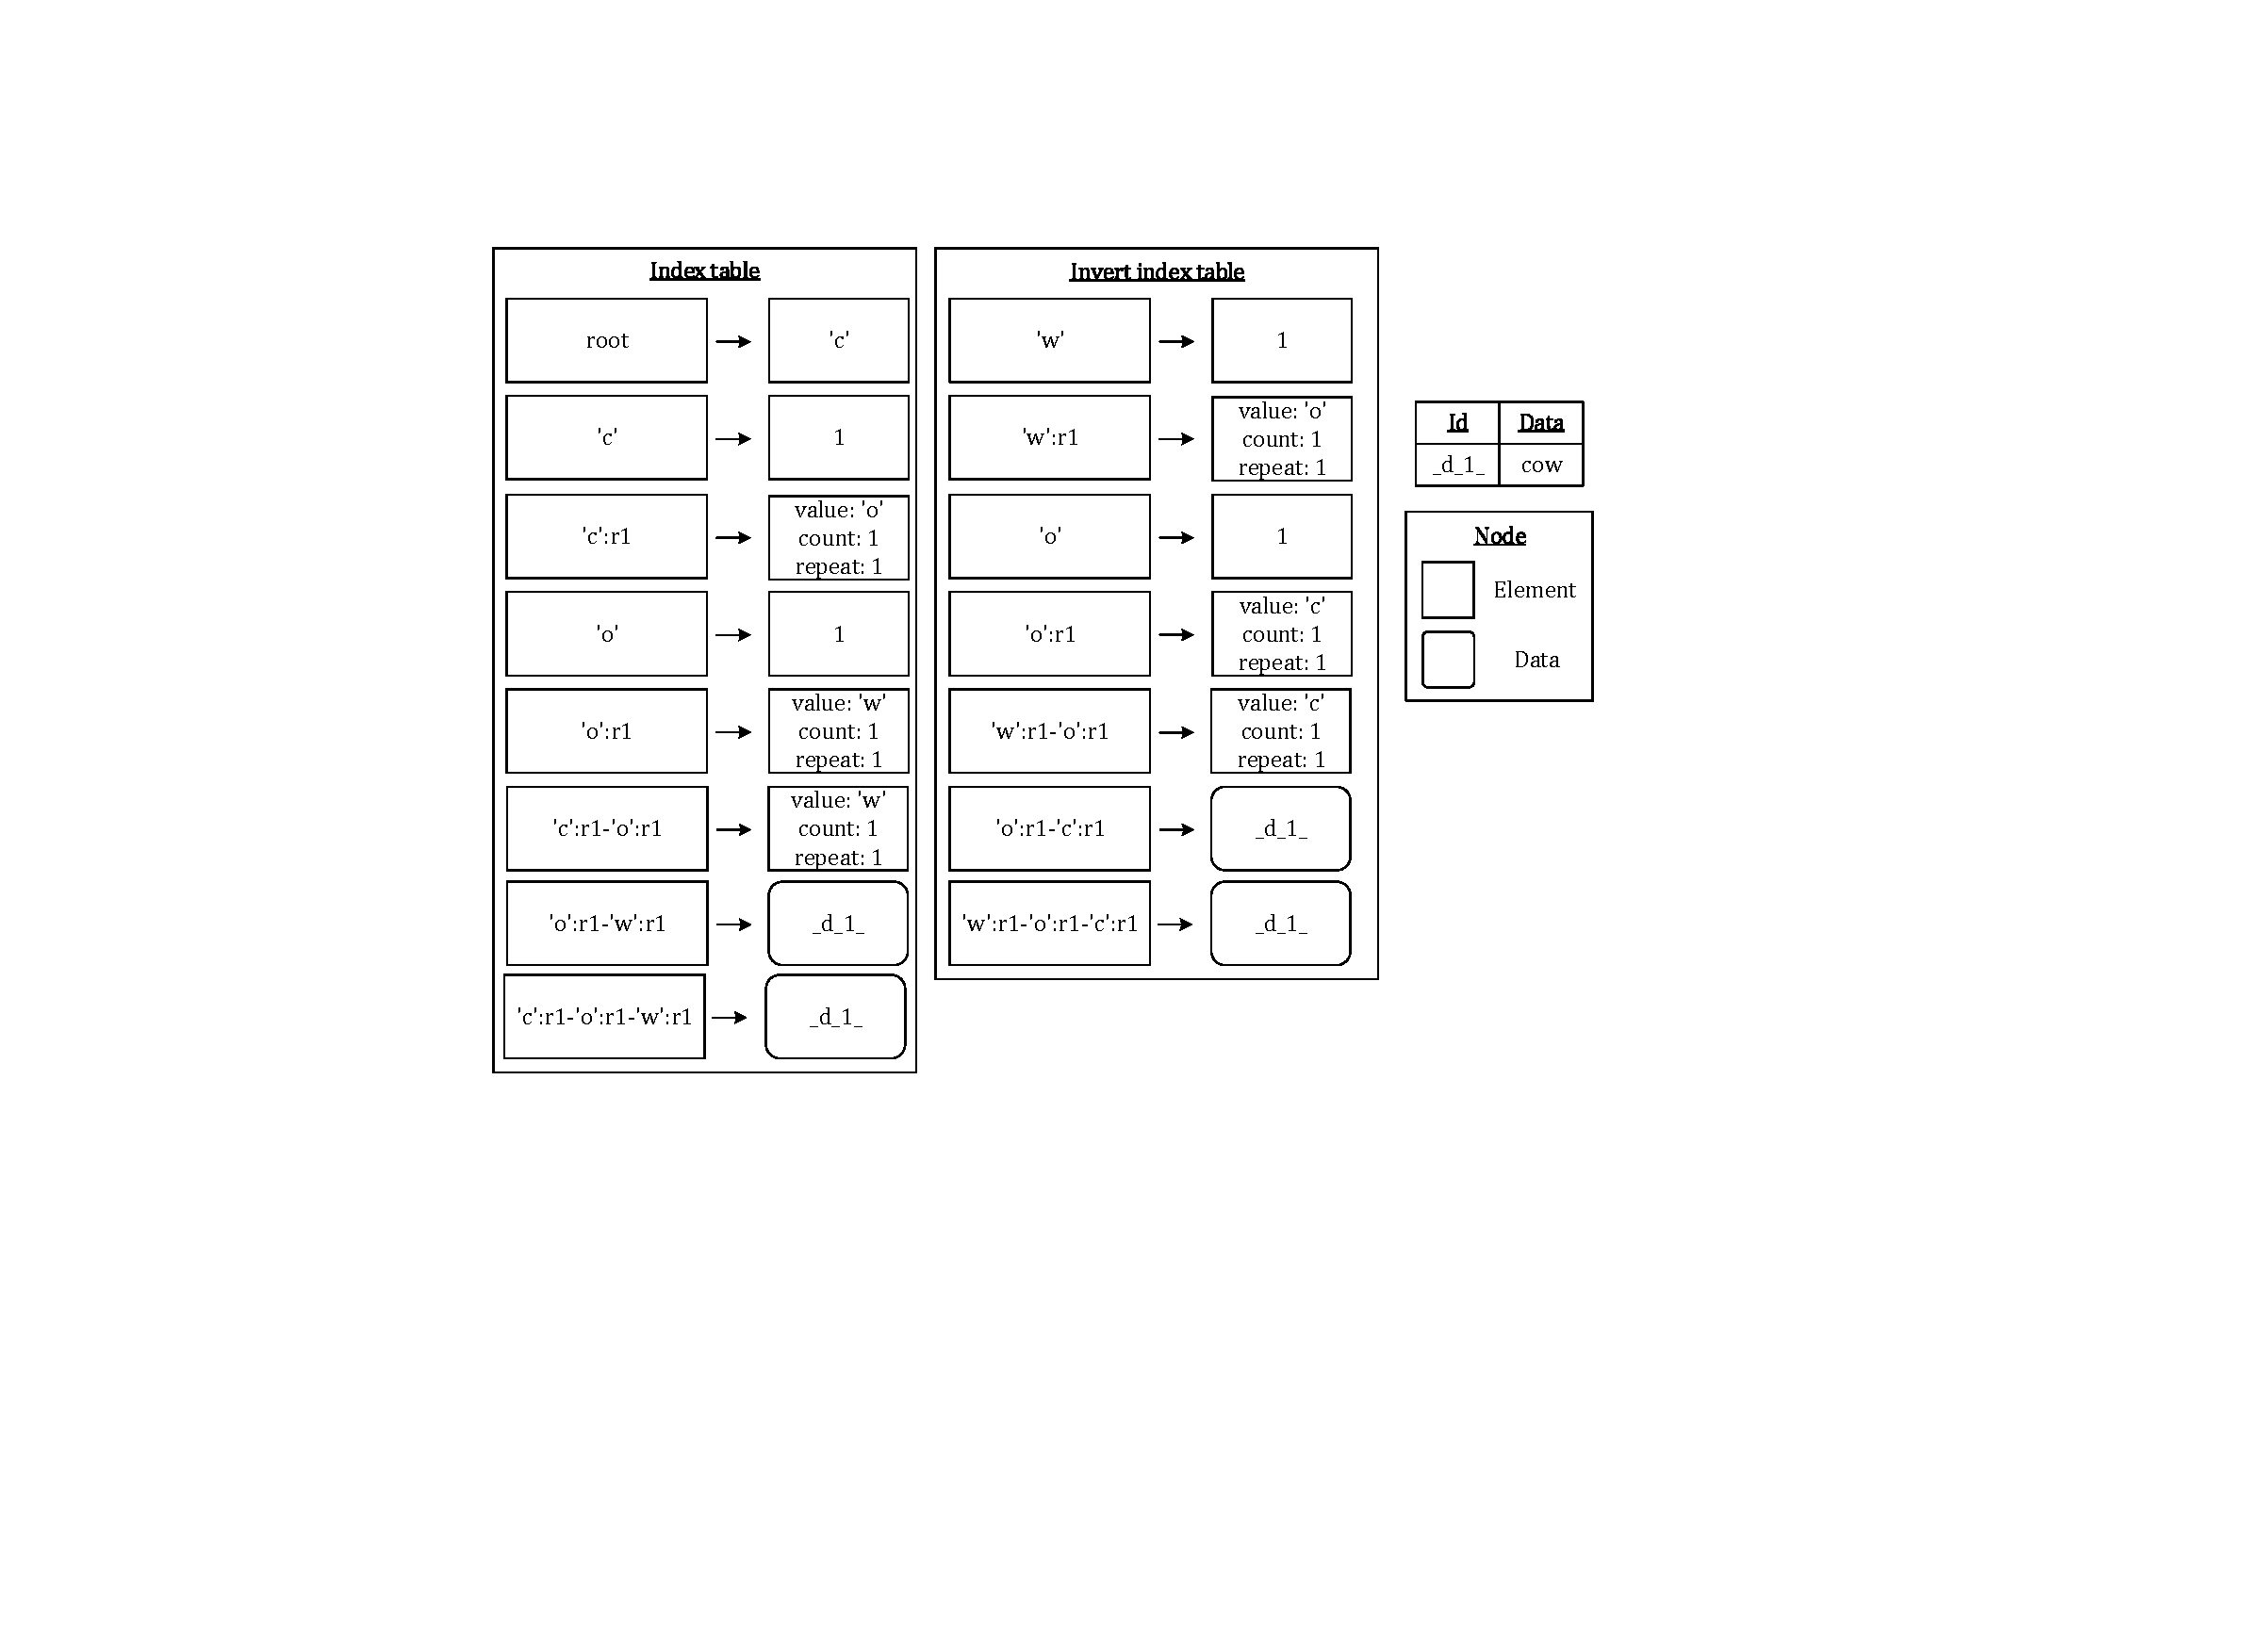
\includegraphics[scale=0.4]{./algorithm/pic/index_table/table_format_v13.pdf}
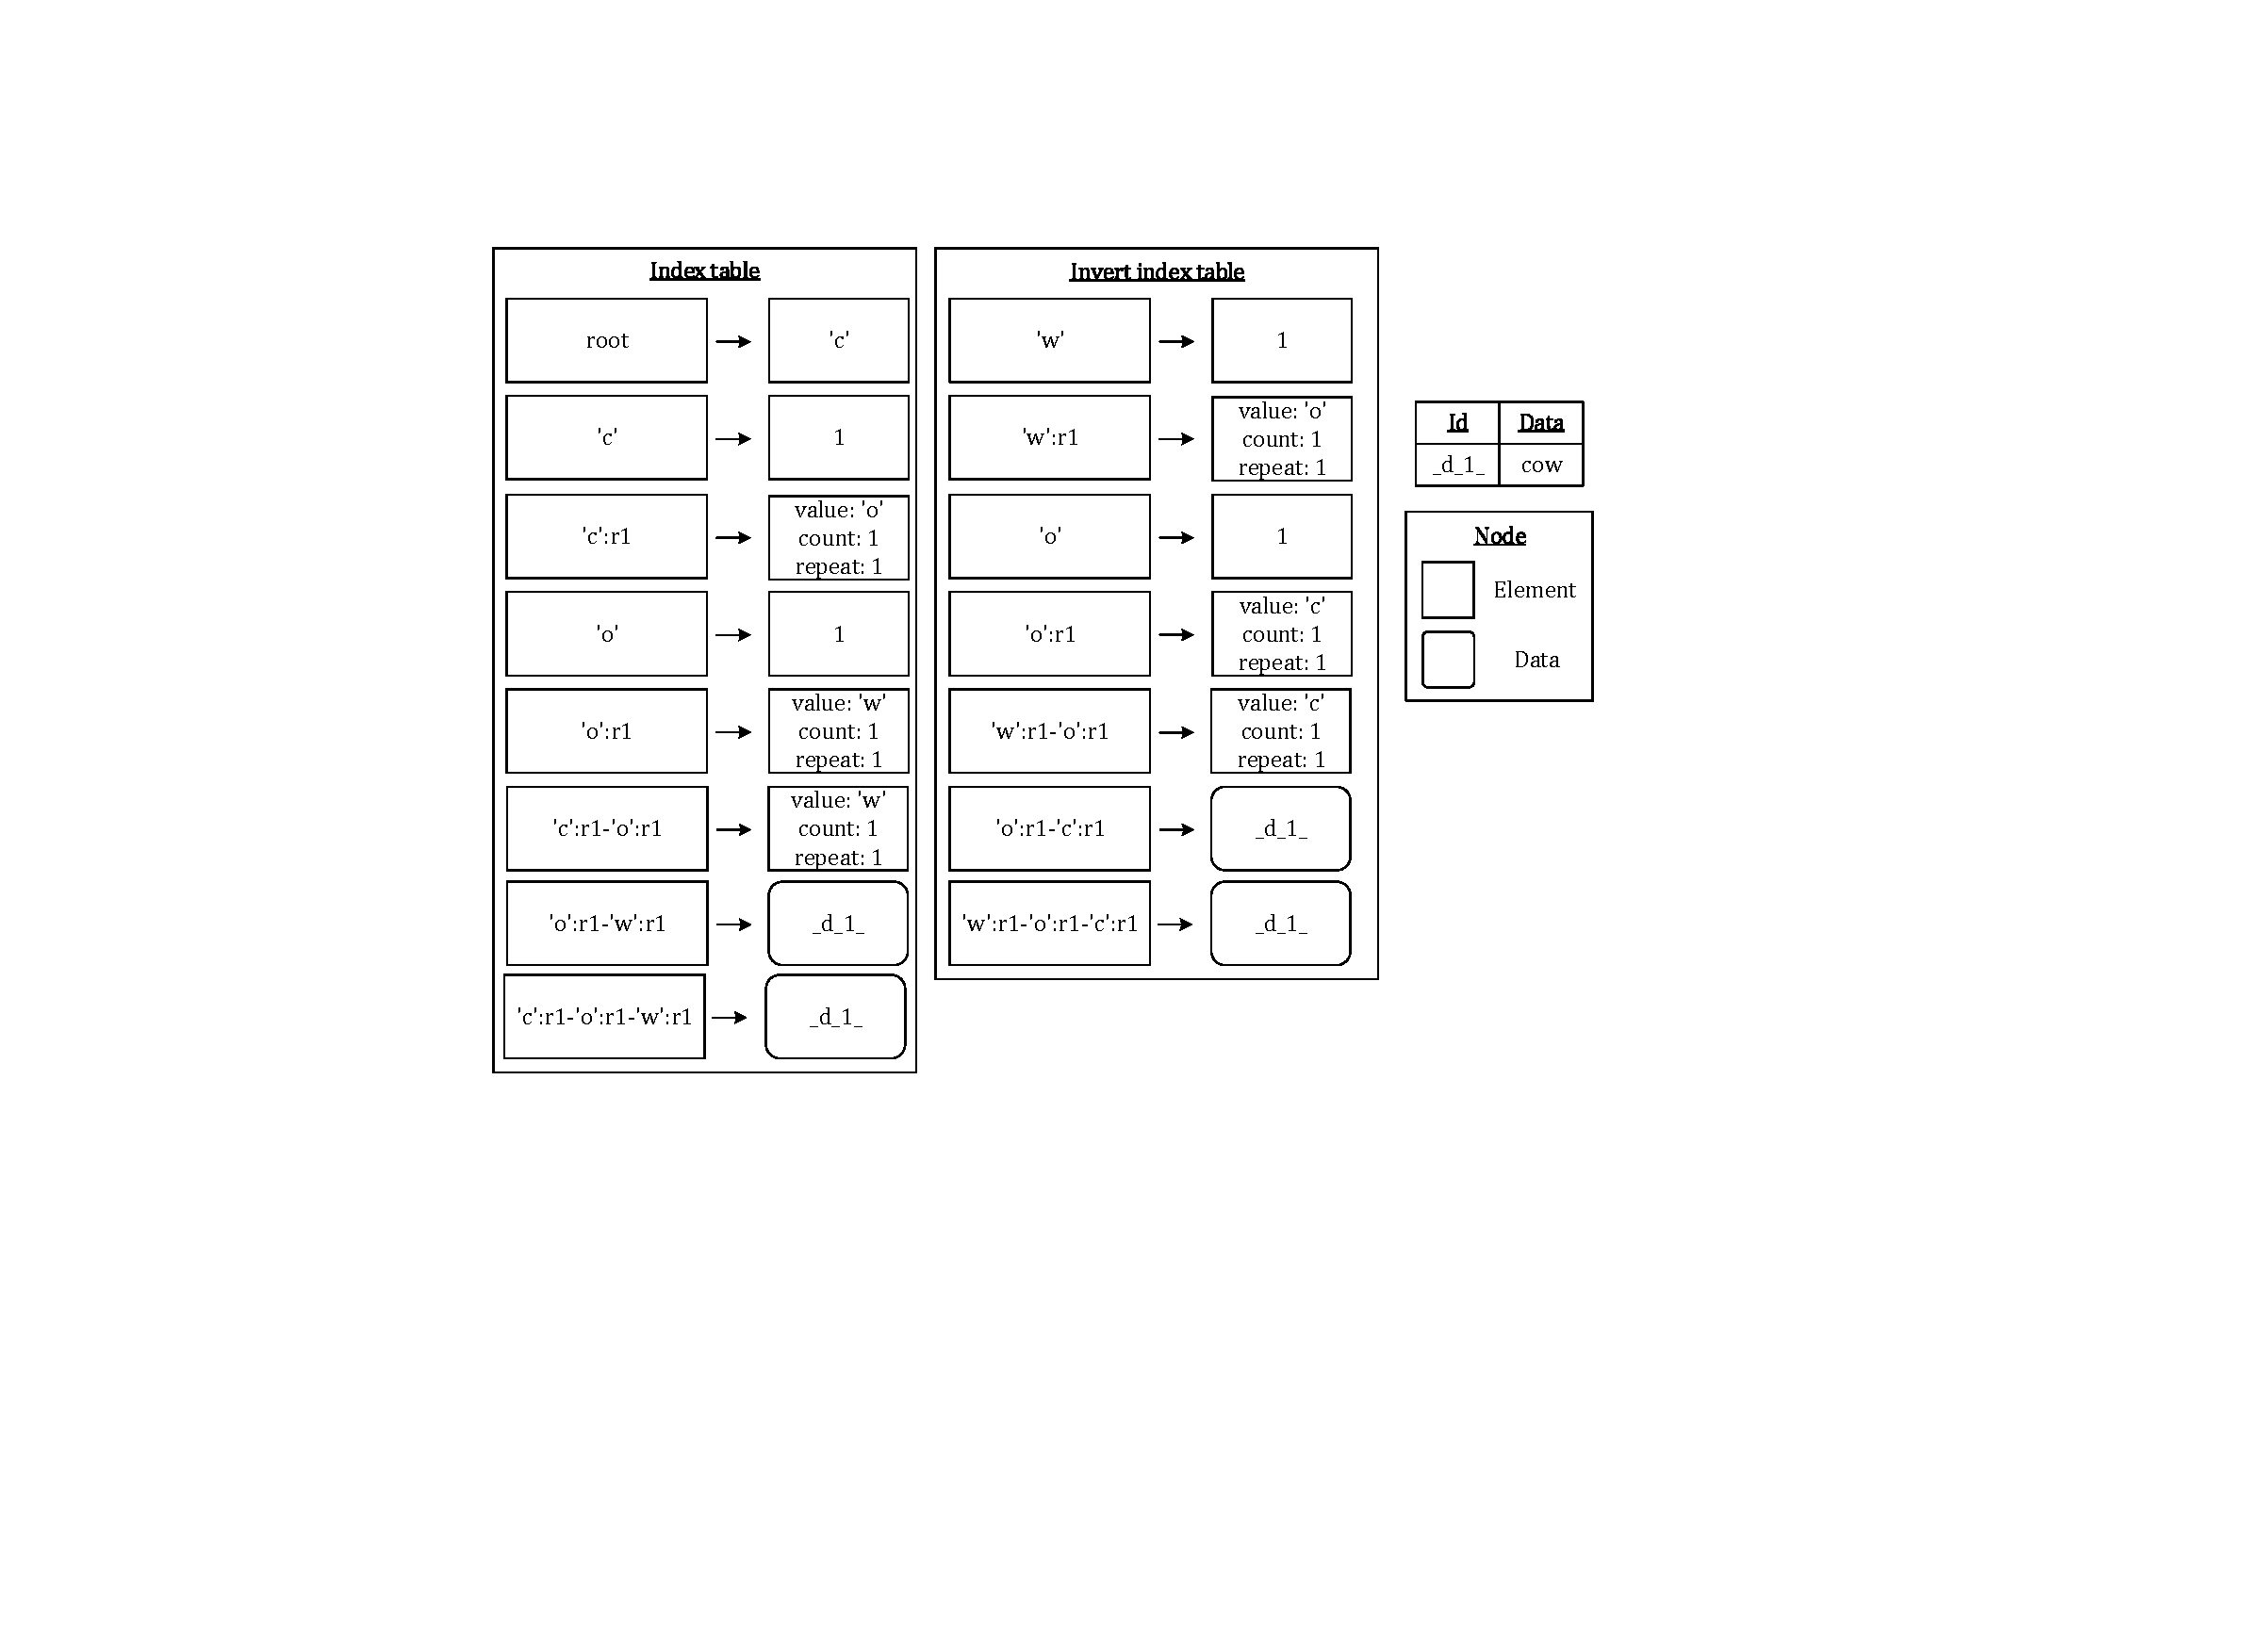
\includegraphics[width=0.8\textwidth]{./algorithm/pic/index_table/table_format_v13.pdf}
\caption{A example of Li's Hash.}
\label{fig:algorithm:lishash_example}
\end{figure}

The time complexity of initial the tables is $O(1)$. About the meanings of all tables, which will more clearly in each operation of all data type.

\clearpage

% STRING section
\subsection{STRING type}

% Insertion section
\subsubsection{Insertion}

When insert a data into the empty table (Figure \ref{fig:algorithm:string:insertion:empty_table}), every data will assign a unique \textit{id} for this data, this \textit{id} will use for the index to look for.

\begin{figure}[h]
\centering
%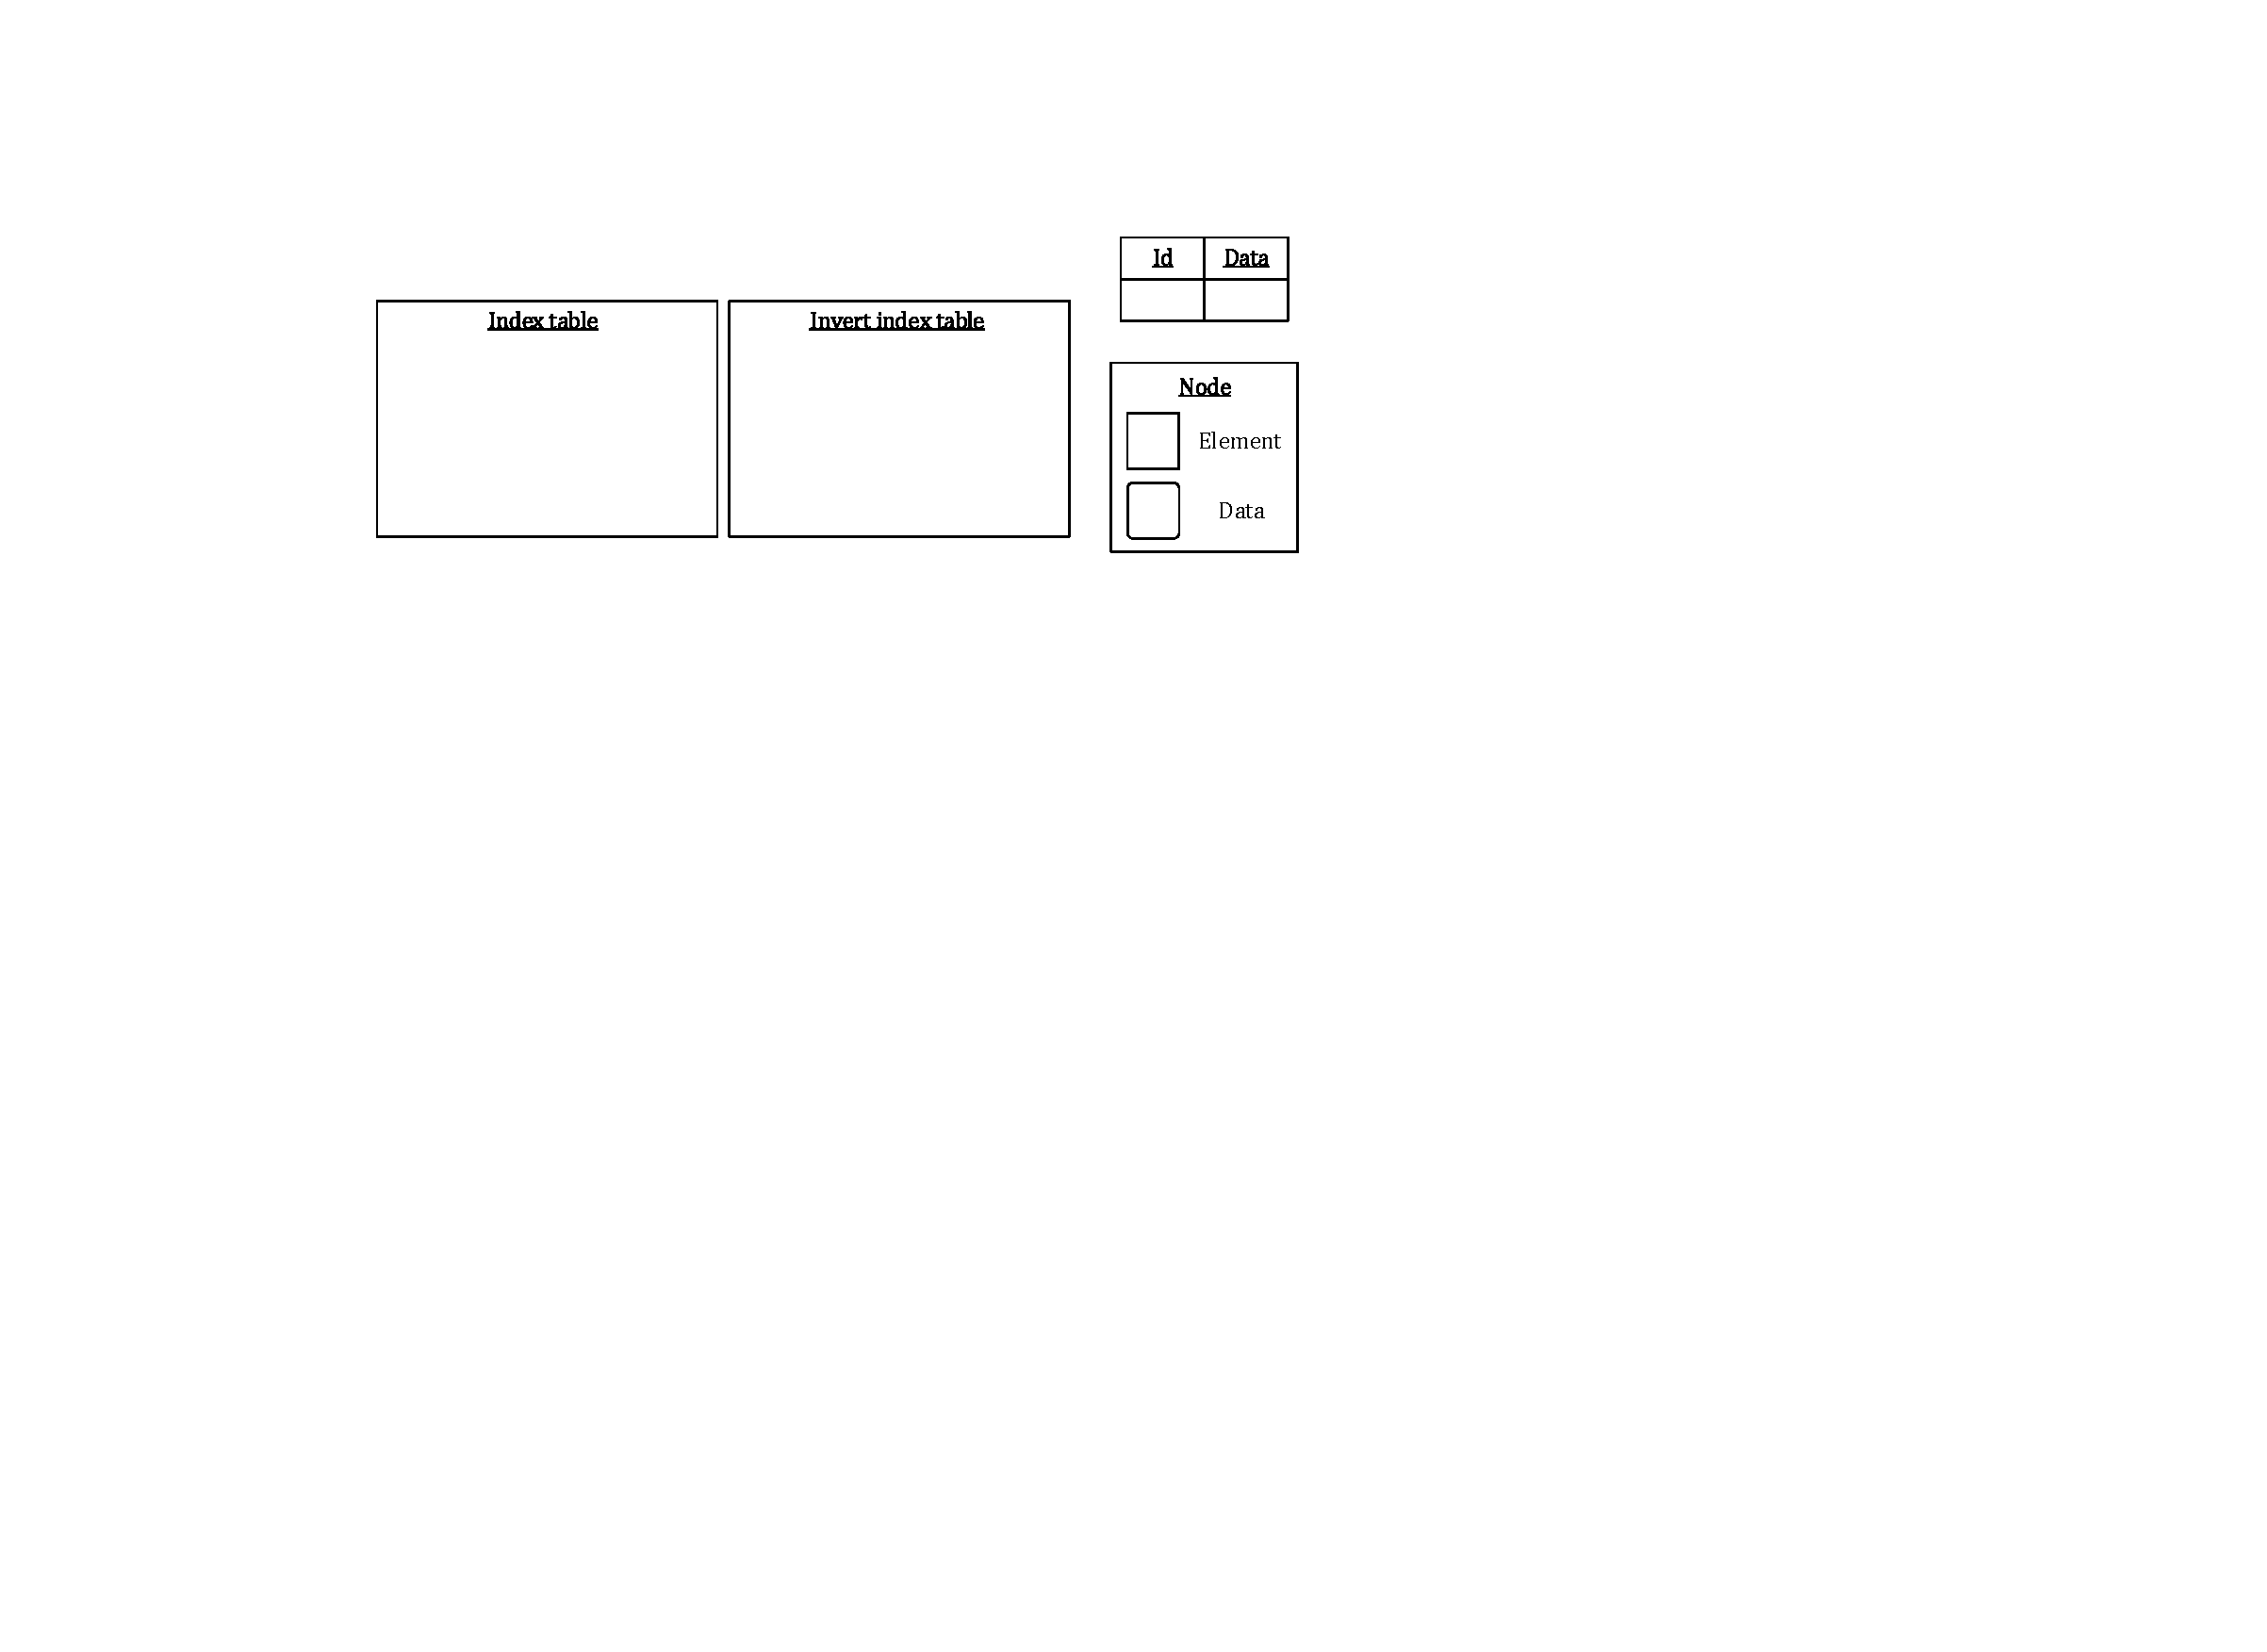
\includegraphics[scale=0.4]{./algorithm/string/pic/insertion/empty_table_v2.pdf}
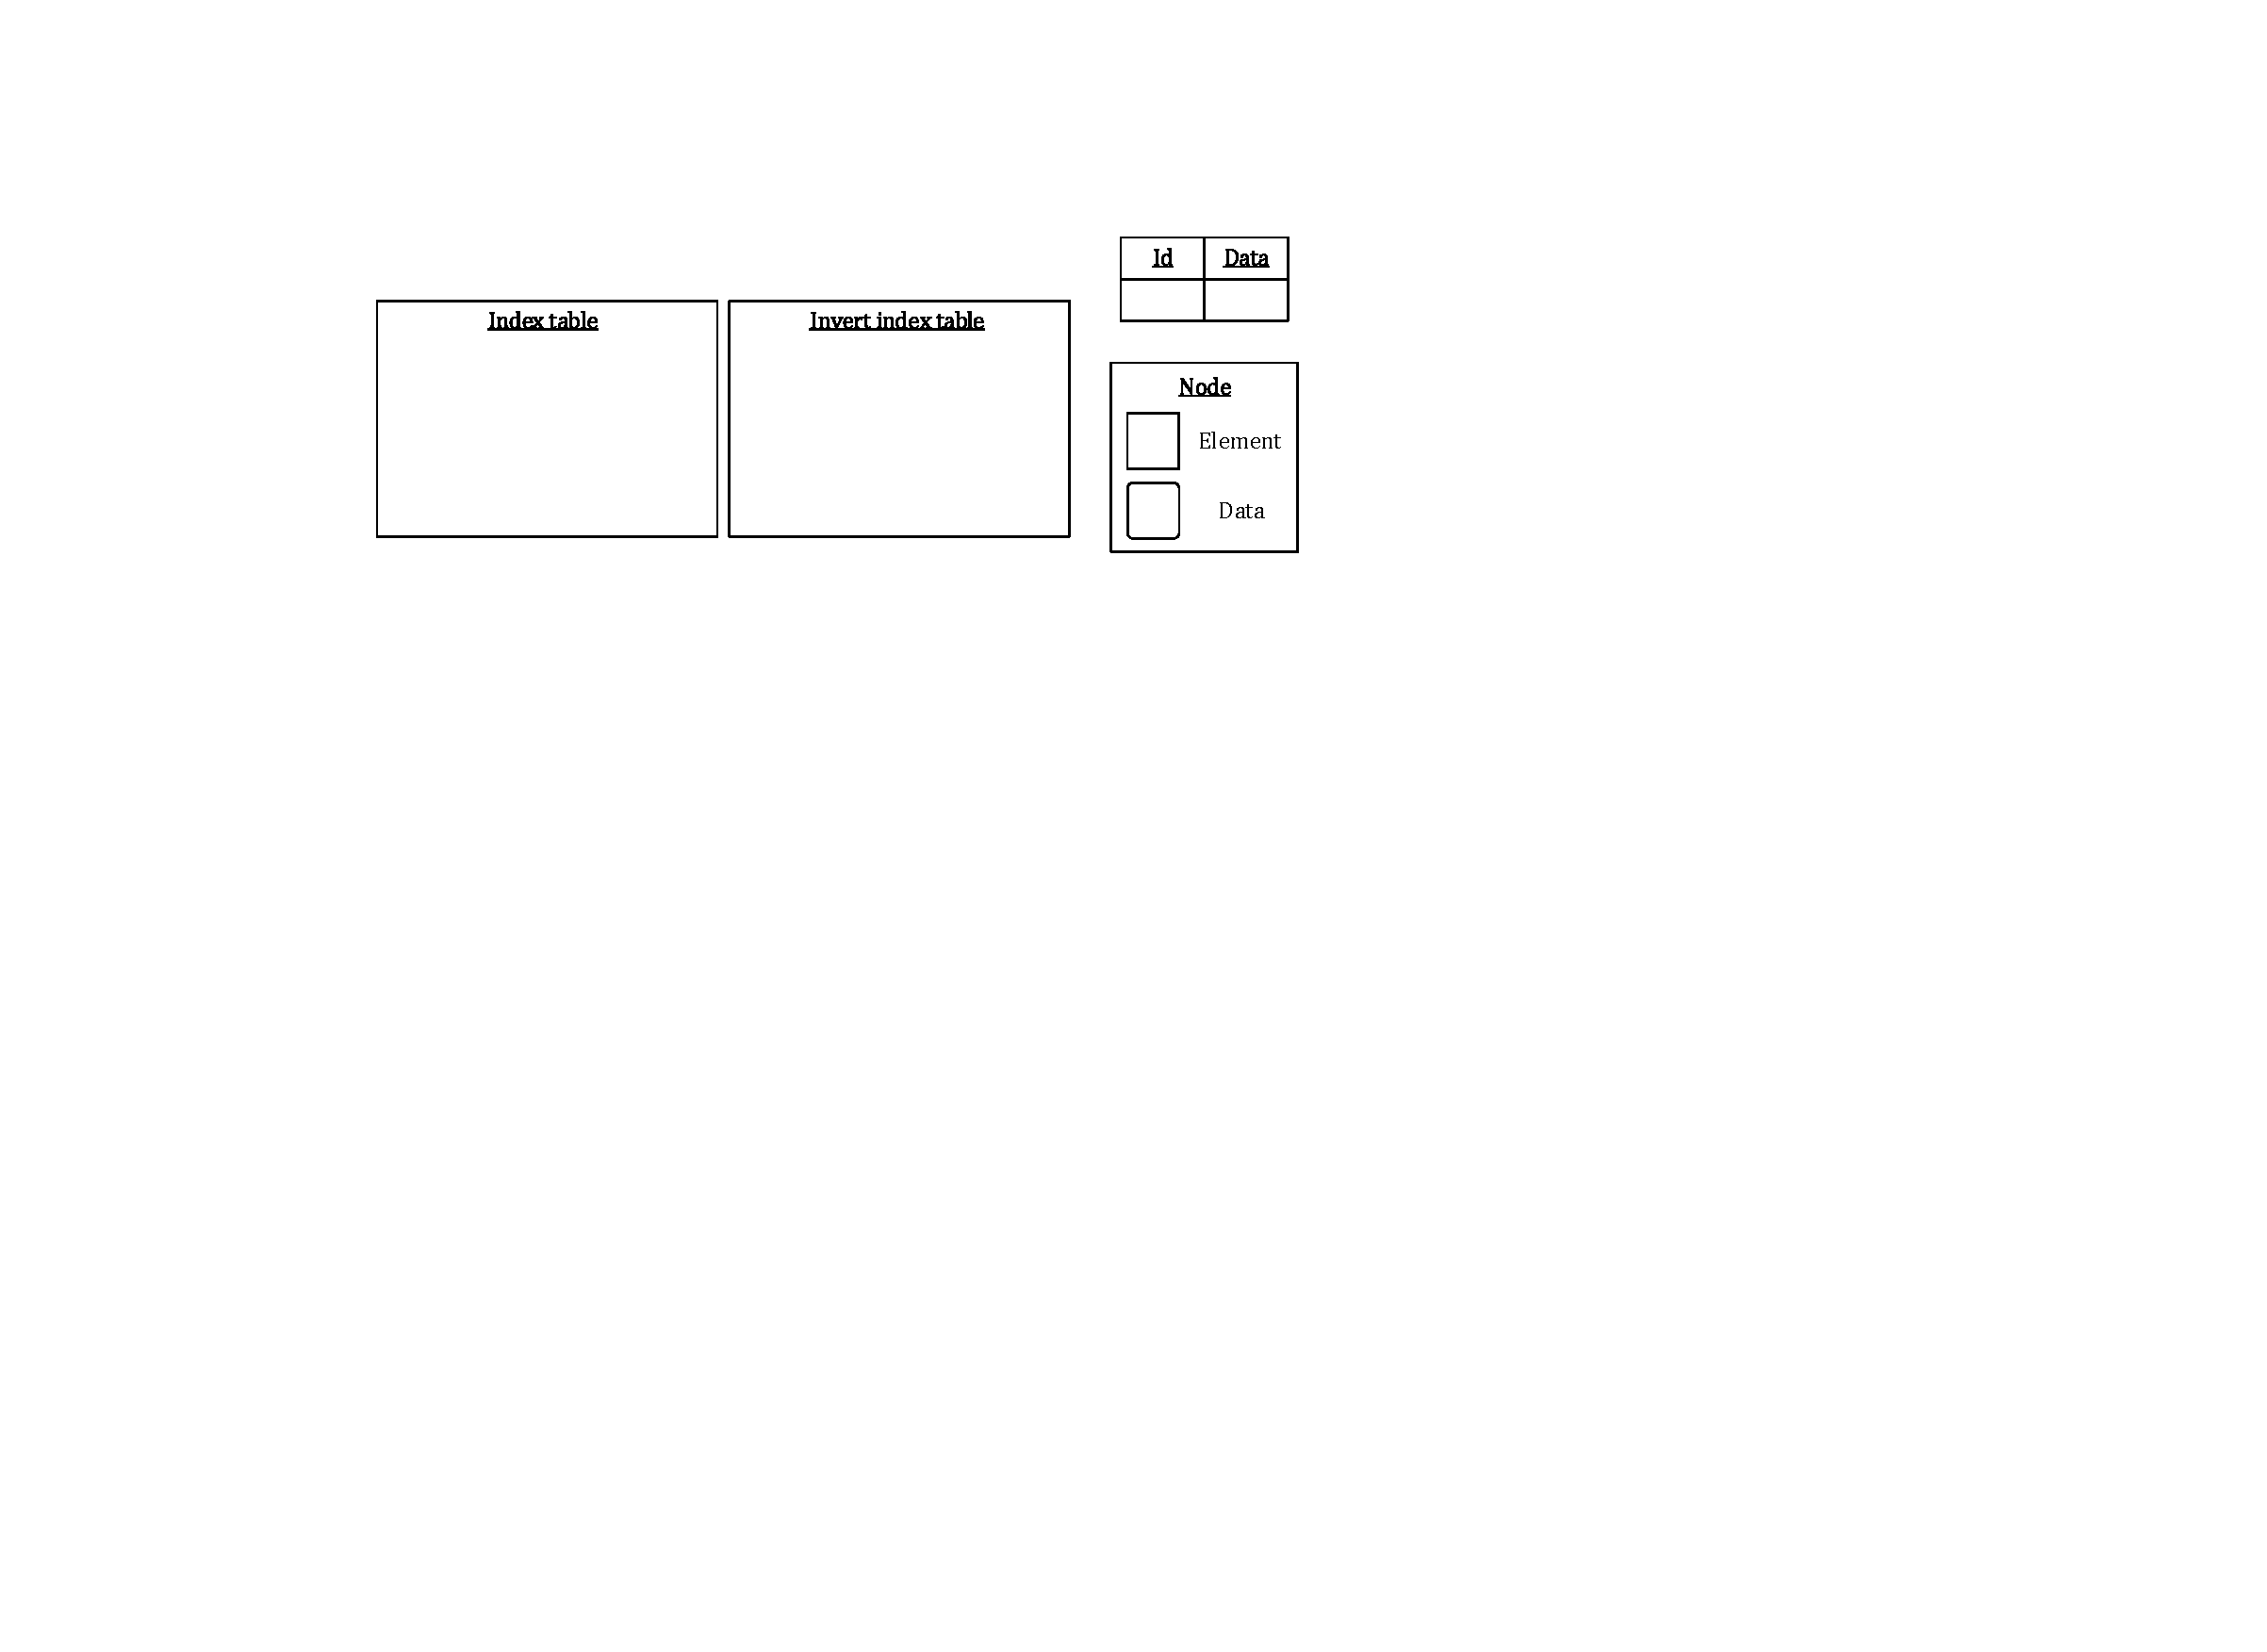
\includegraphics[width=0.5\textwidth]{./algorithm/string/pic/insertion/empty_table_v2.pdf}
\caption{A empty index table.}
\label{fig:algorithm:string:insertion:empty_table}
\end{figure}

So for example if inputting a data \textit{"book"}, first assign the \textit{id} as \textit{"\_d\_1\_"}, next step is separate the bytes using n-gram indexing with counting the repeat value to from the keys. So \textit{"book"} can count as \textit{b-\textgreater1}, \textit{o-\textgreater2} and \textit{k-\textgreater1} by counting the repeat value. And formed into \textit{"b"}, \textit{"bo"}, \textit{"boo"}, \textit{"book"}, \textit{"oo"}, \textit{"ook"} by n-gram but because using count the repeat byte that \textit{"bo"} is domained by \textit{"boo"}.\\

Every byte will have their own key such as \textit{'b'} and \textit{'o'} for record their repeat count, which is using in searching to know there have the keys like \textit{"'b':r1"} or \textit{"'o':r2"} which can use. The \textit{'r'} in key means the repeat times of that value. But the last byte wouldn't have that key in index table because of the key will exist in invert index table, also this happen in the opposite.\\

So the data will index as figure \ref{fig:algorithm:string:insertion:example_1}.

\begin{figure}[h]
\centering
%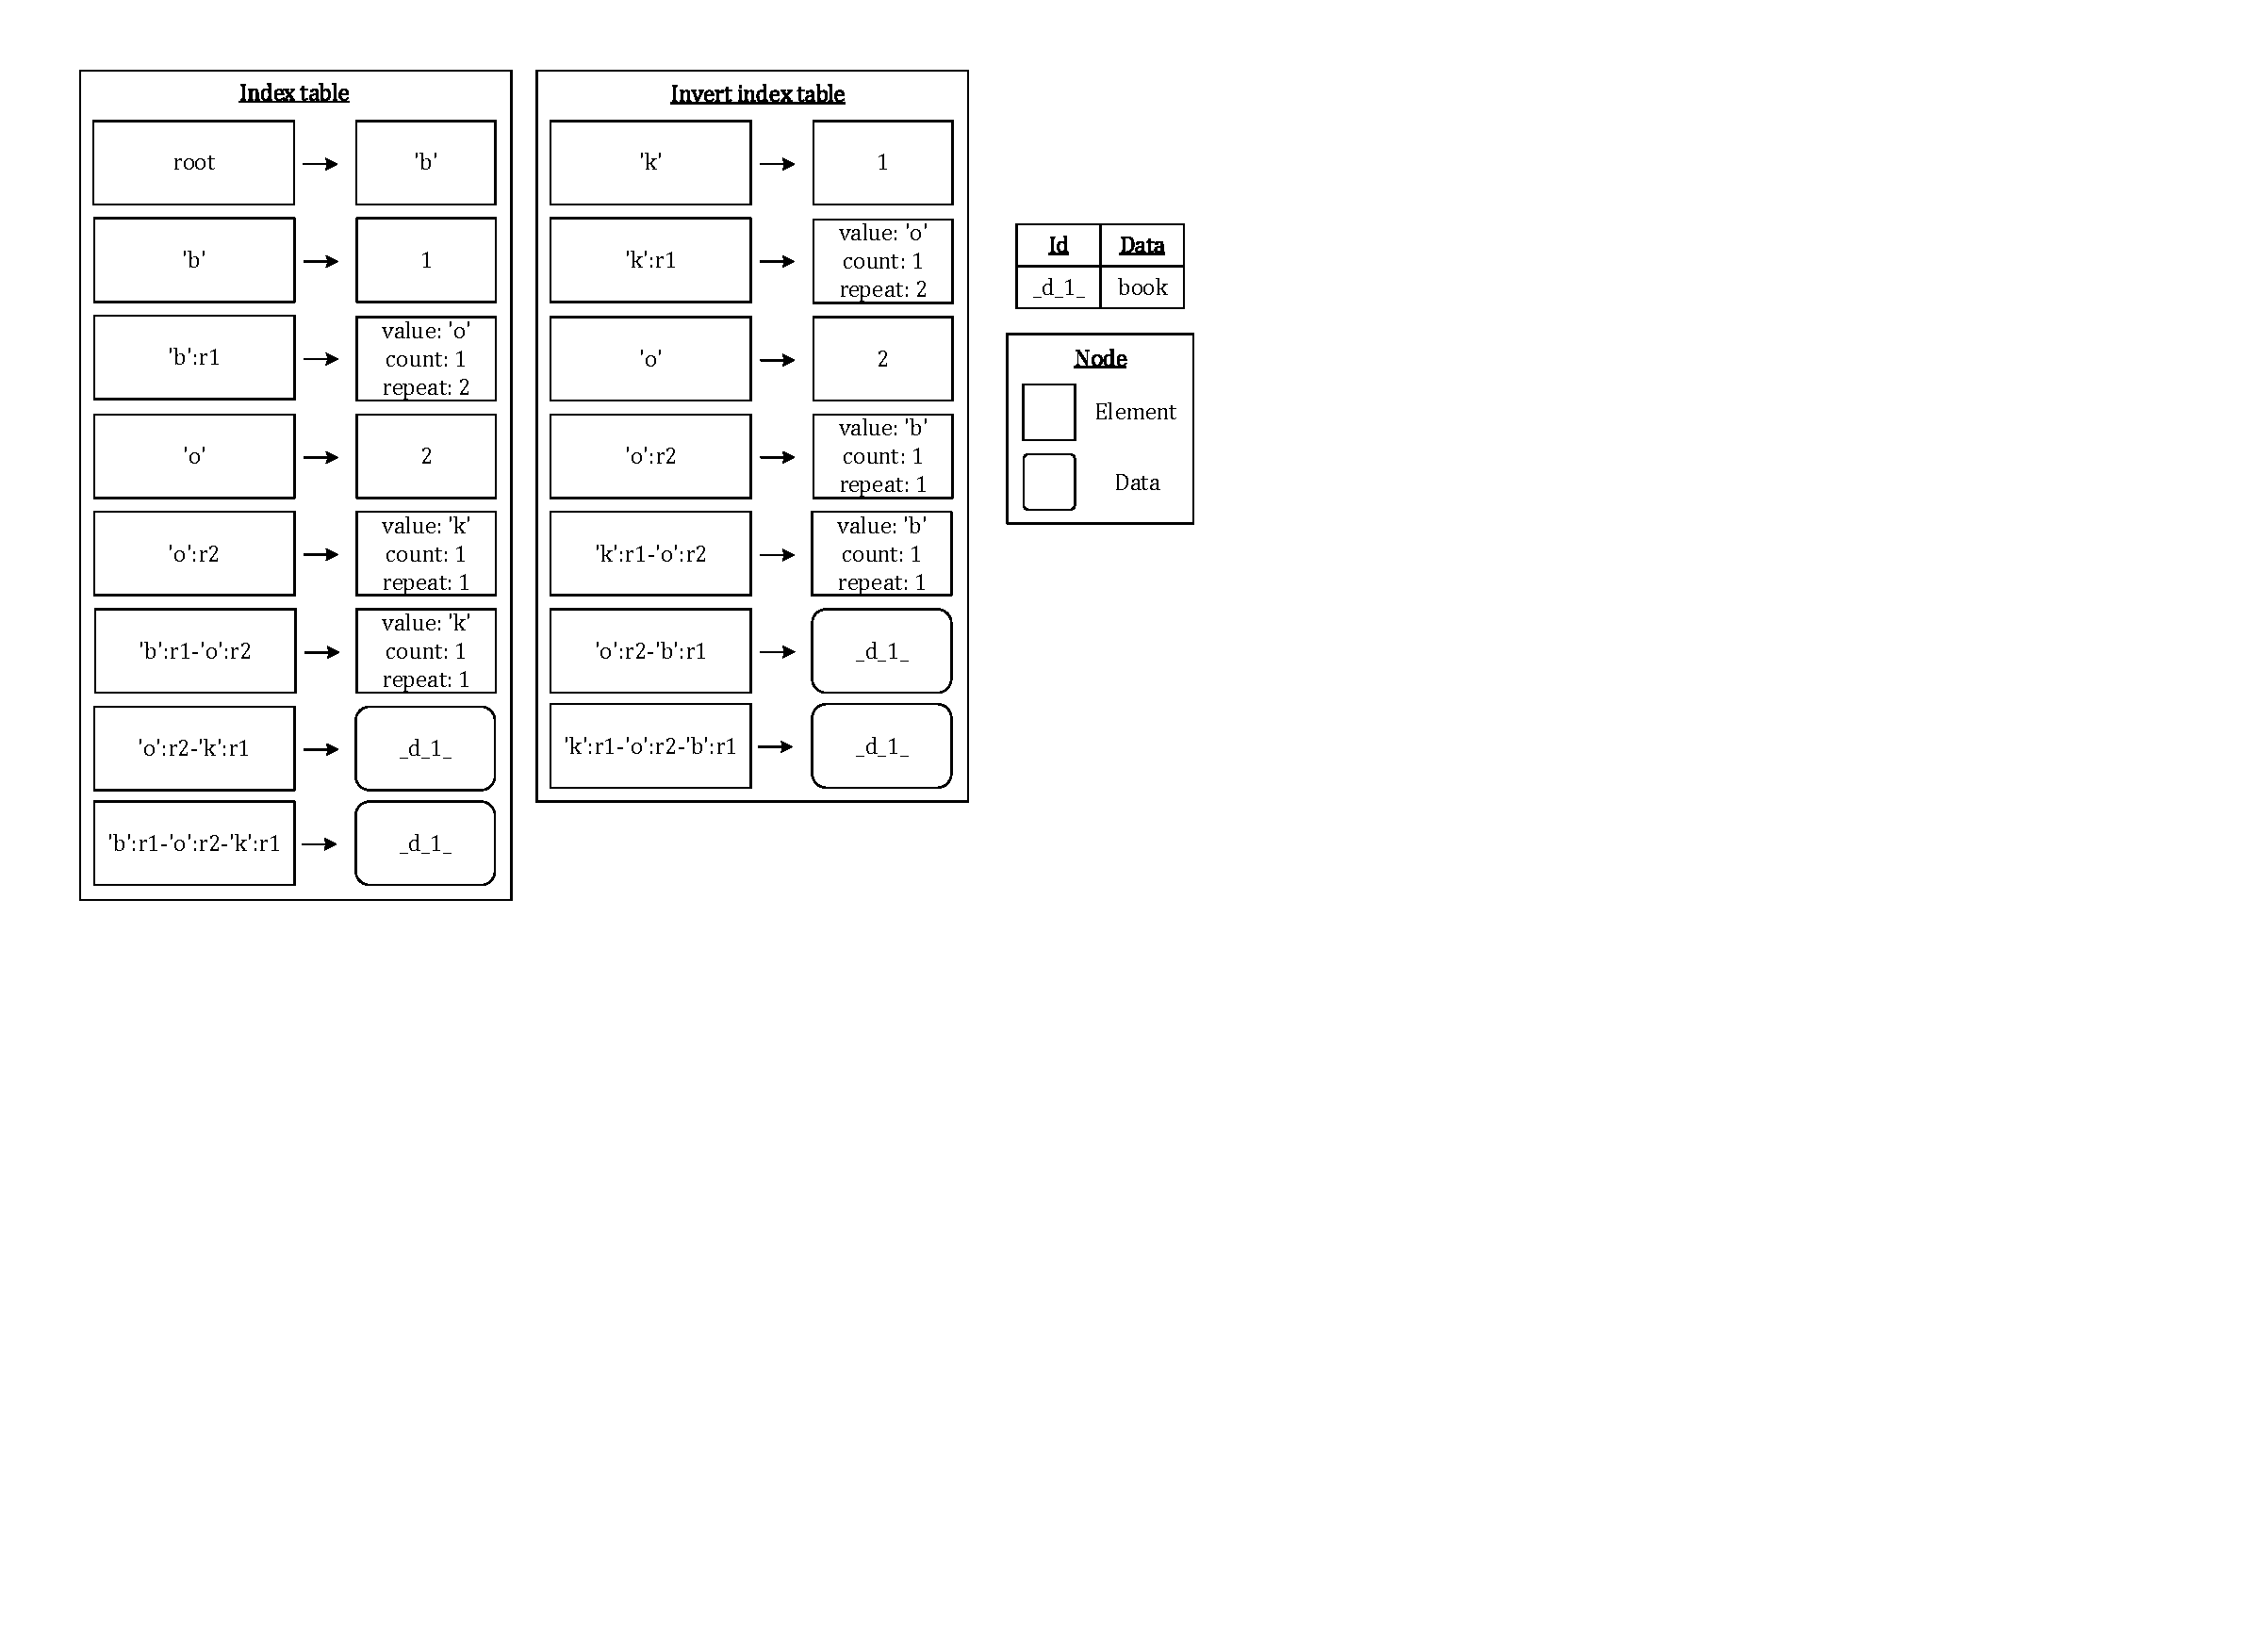
\includegraphics[scale=1.0]{./algorithm/string/pic/insertion/example_1_v5.pdf}
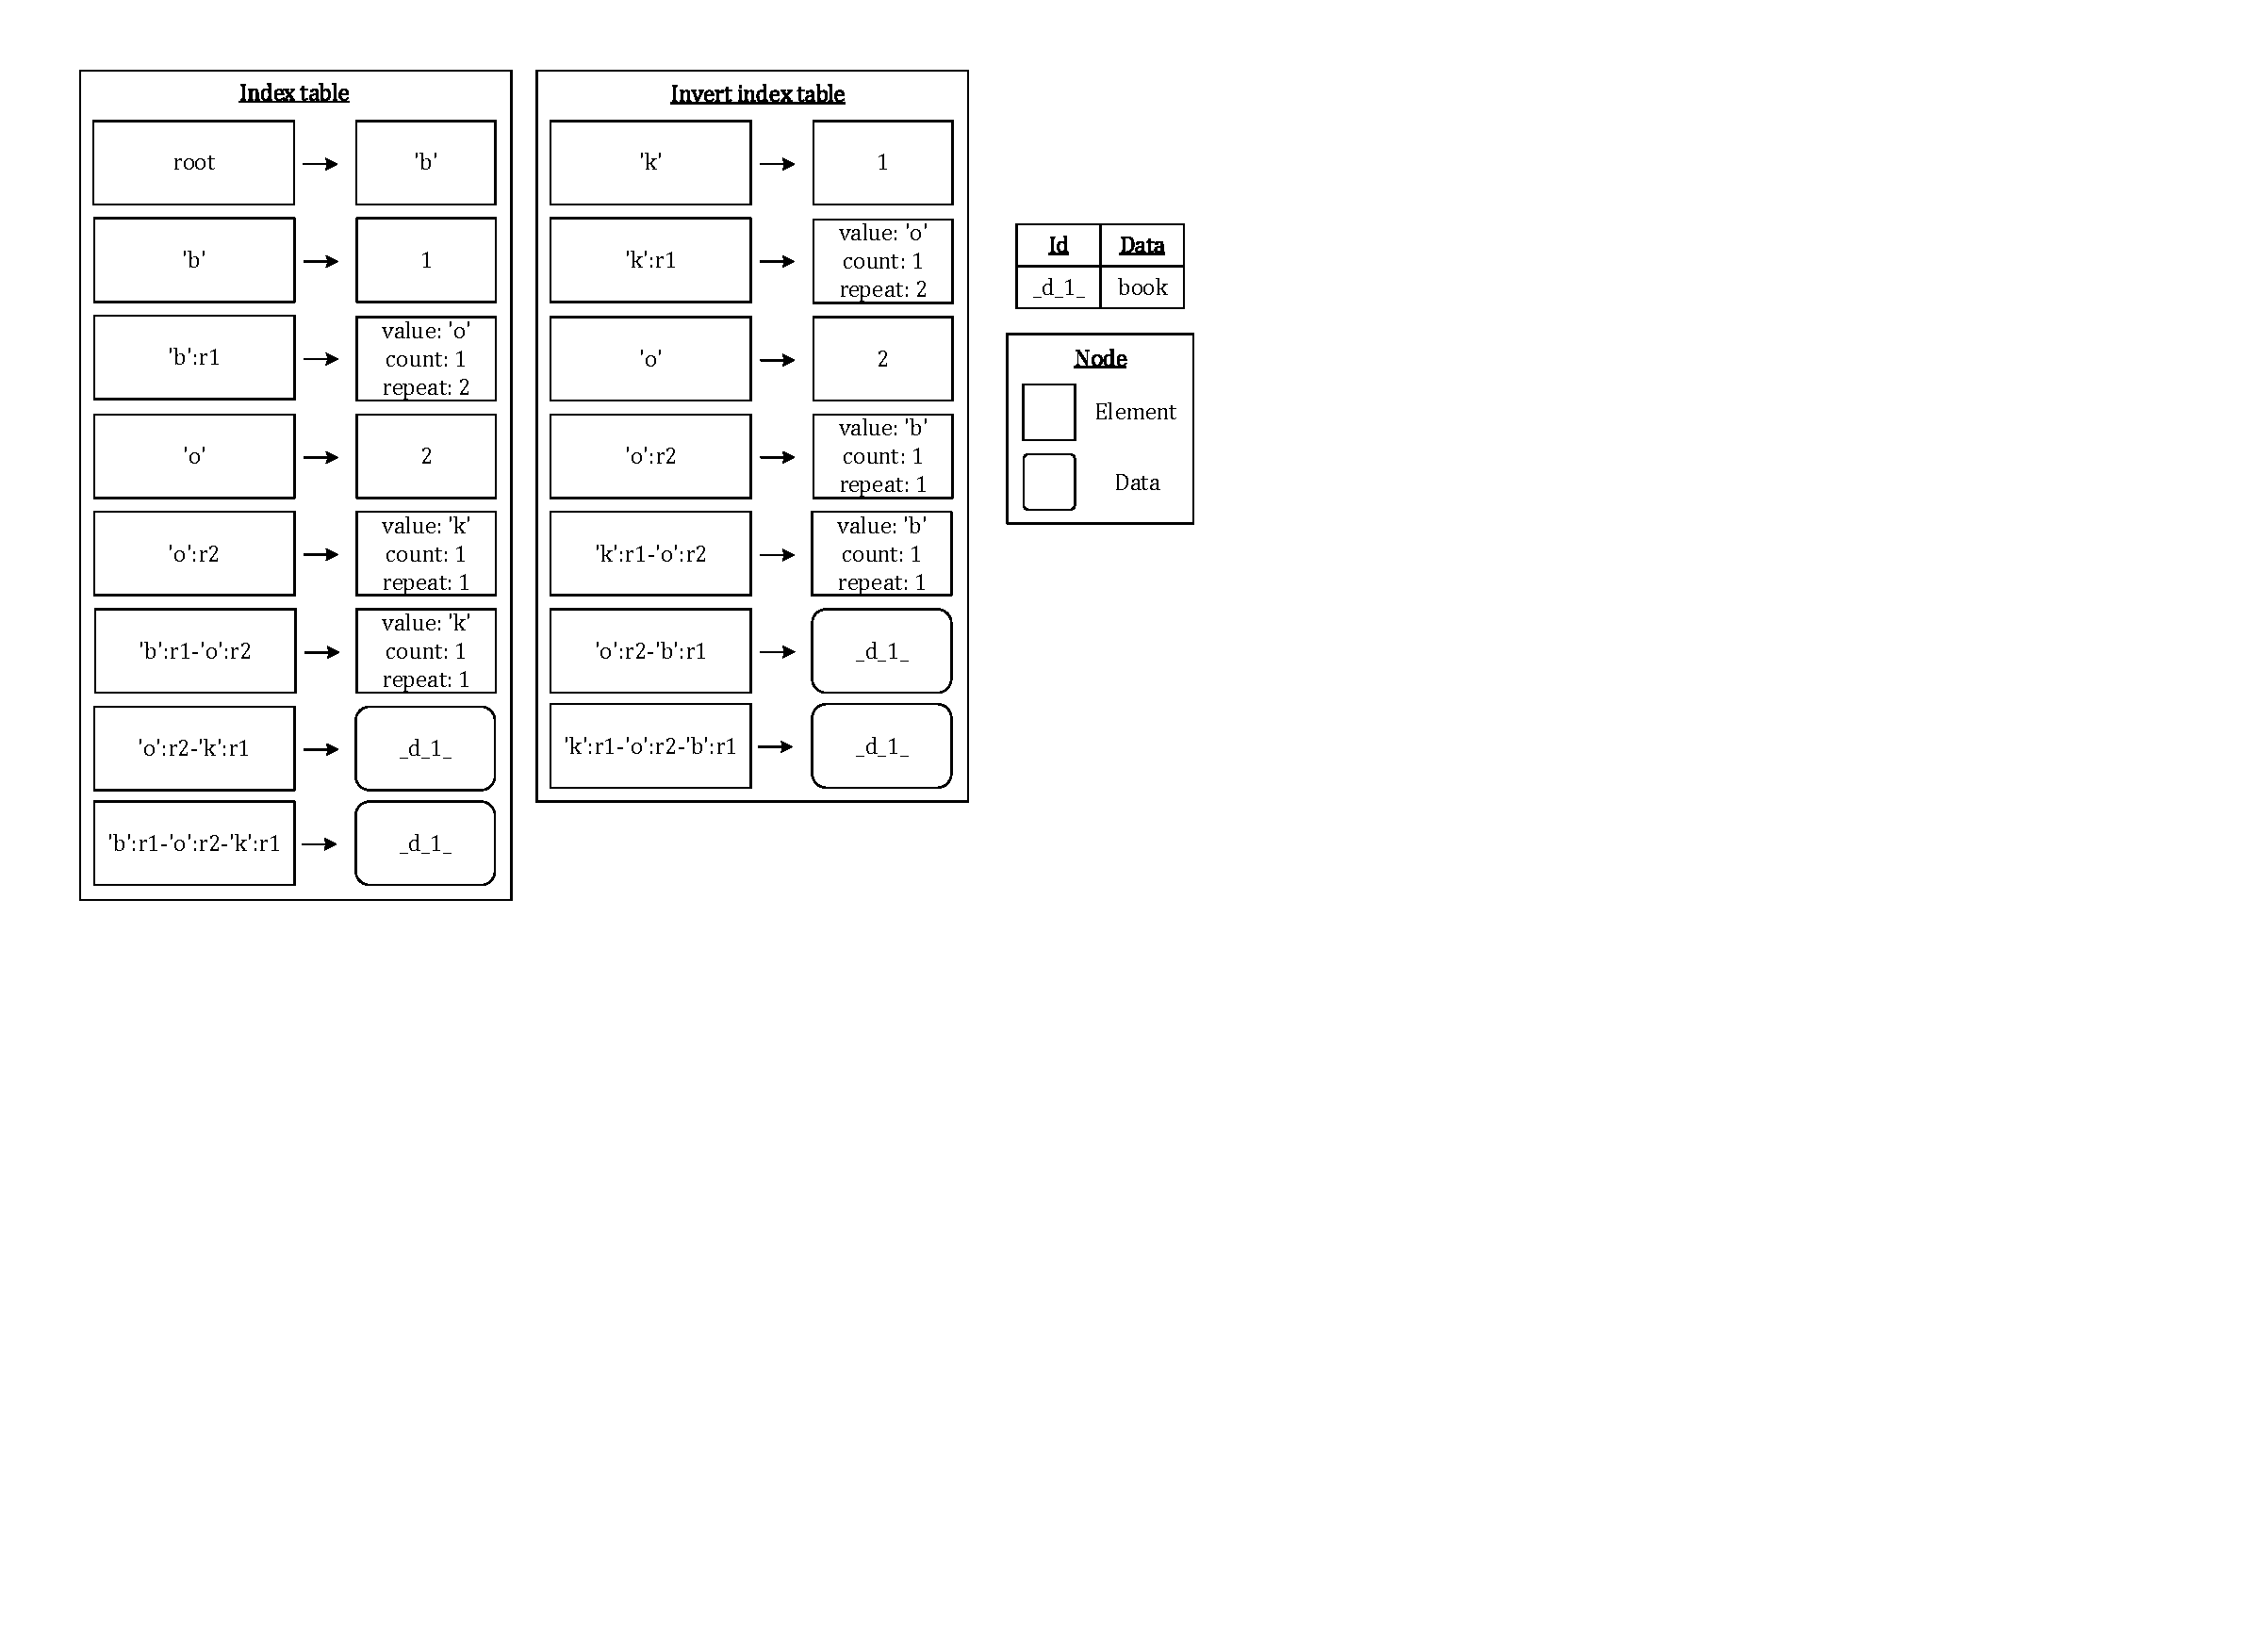
\includegraphics[width=0.7\textwidth]{./algorithm/string/pic/insertion/example_1_v5.pdf}
\caption{Insert data "book".}
\label{fig:algorithm:string:insertion:example_1}
\end{figure}

The time complexity of insertion should look like figure \ref{fig:algorithm:string:insertion:time_complexity}. The time complexity of insert a data should be $O(b)$, $b!$ is the number of for loop which is equal to the byte length of data, and $O(1)$ is means the key of the data like \textit{"'b':r1-'o':r2-'k':r1"} in the example.\\

\begin{figure}[h]
\centering
%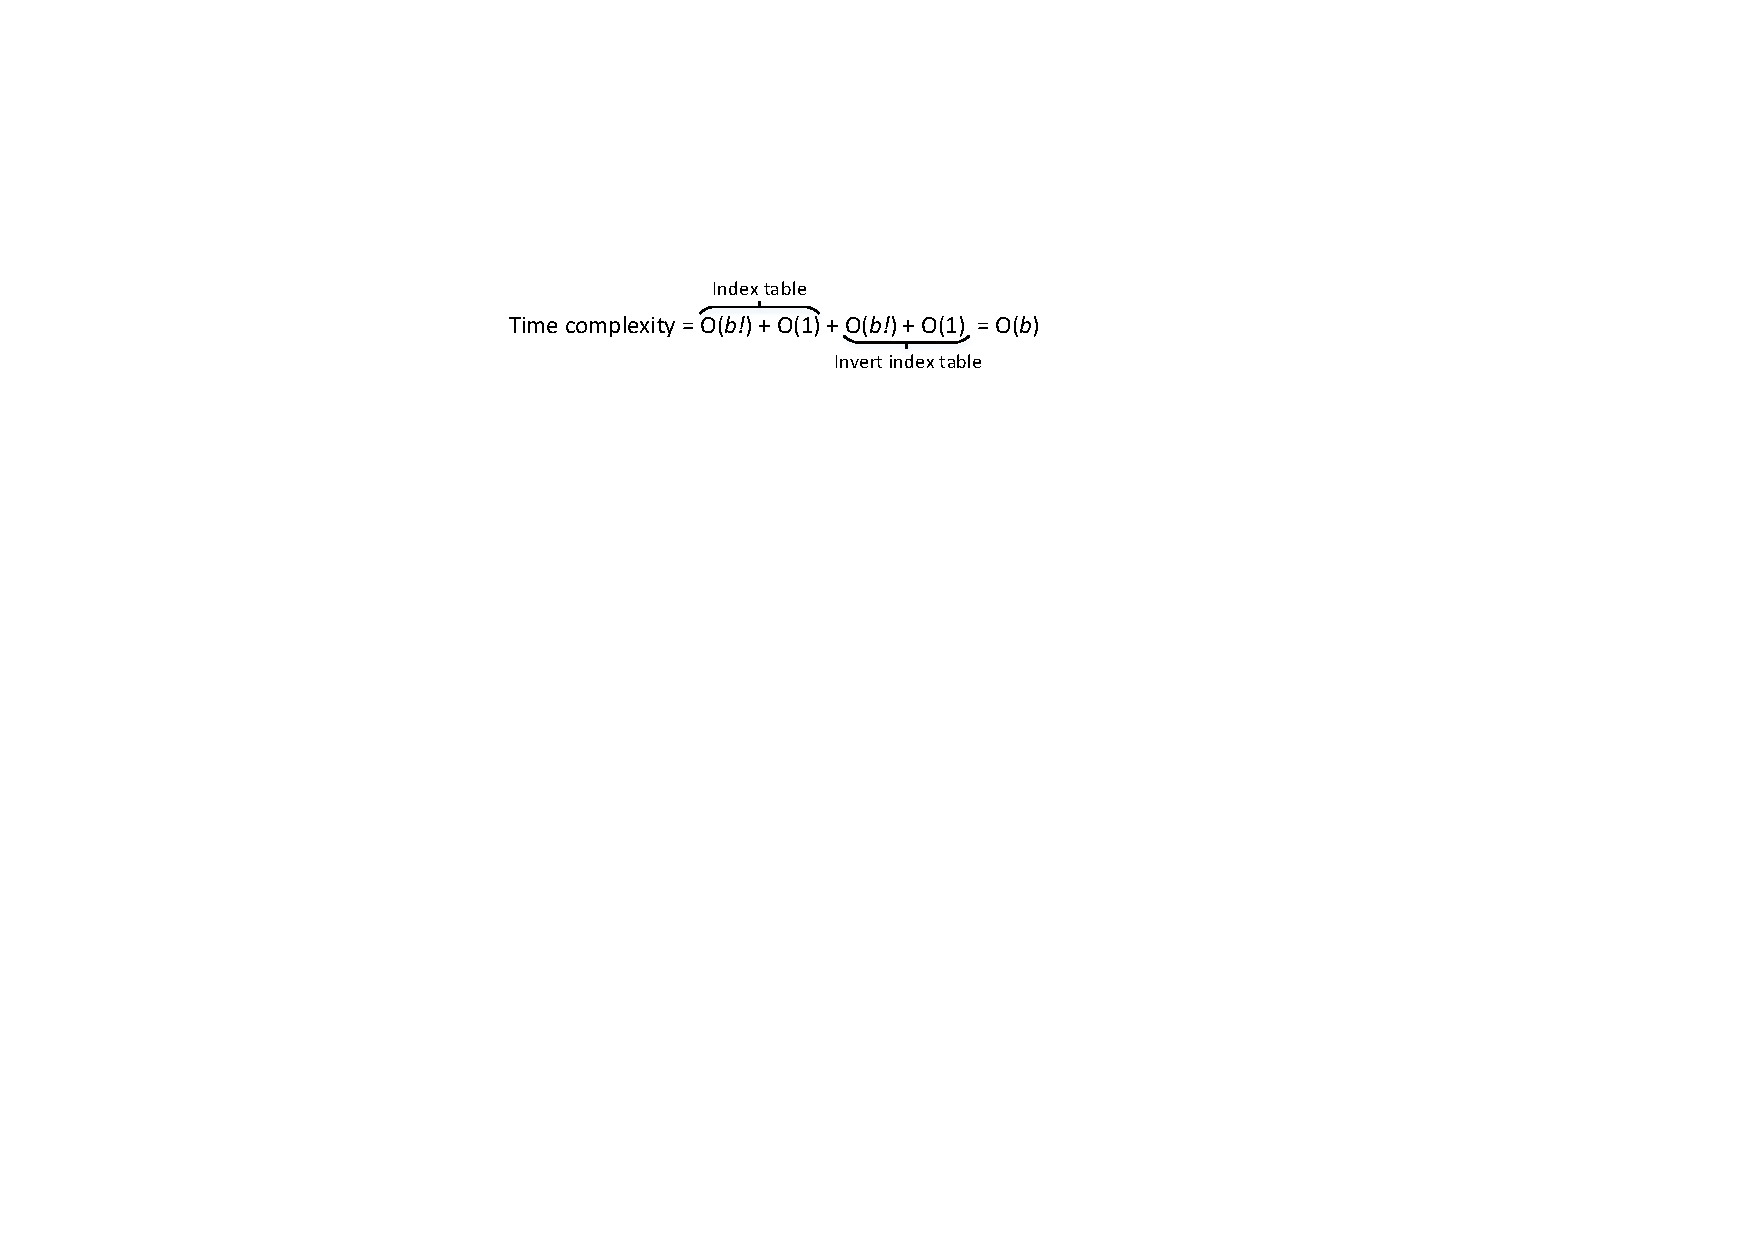
\includegraphics[scale=1.0]{./algorithm/string/pic/insertion/time_complexity_v5.pdf}
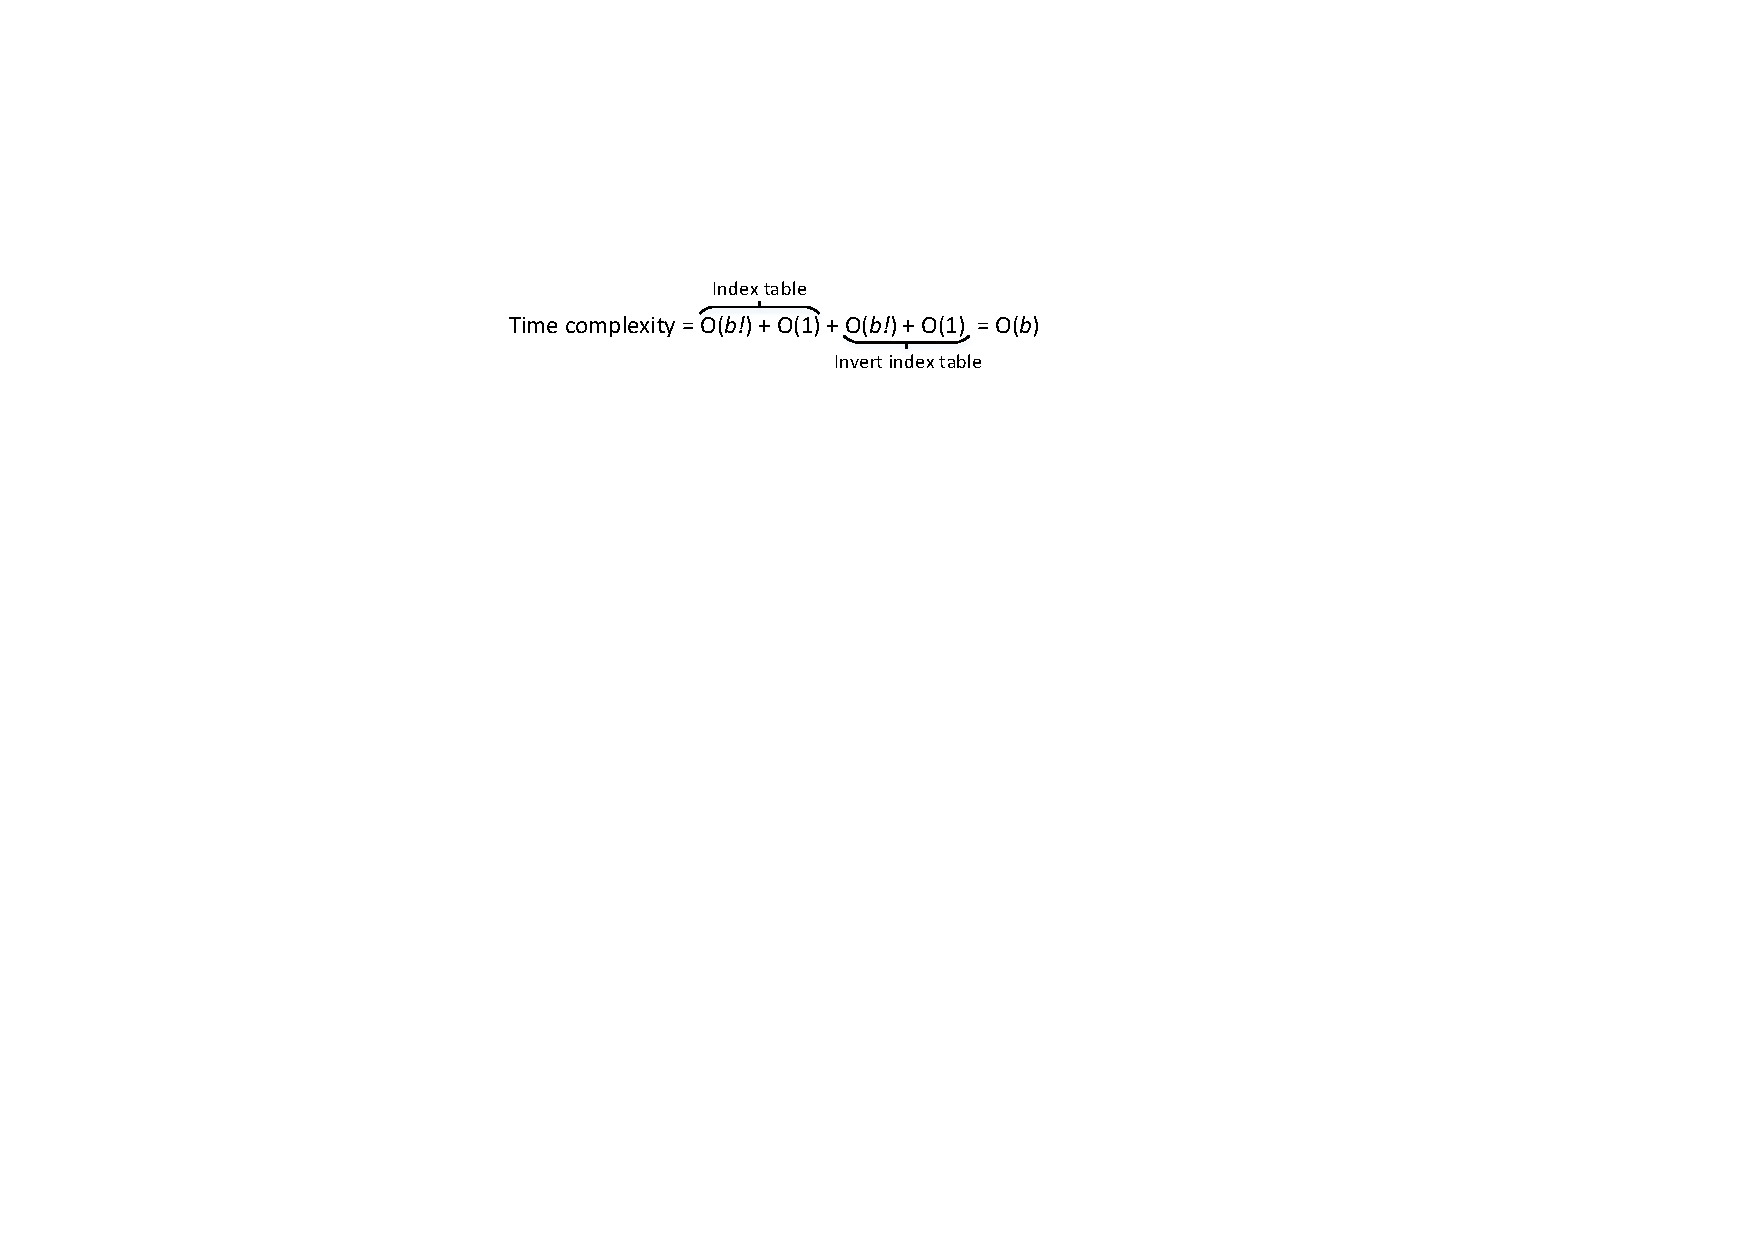
\includegraphics[width=0.6\textwidth]{./algorithm/string/pic/insertion/time_complexity_v5.pdf}
\caption{Time complexity of insertion.}
\label{fig:algorithm:string:insertion:time_complexity}
\end{figure}

Next if insert the data \textit{"box"}, the tables will look like figure \ref{fig:algorithm:string:insertion:example_2}. As the figure shows that \textit{"box"} and \textit{"book"} have a common key, so some of the node will deduplicated.

\begin{figure}[h]
\centering
%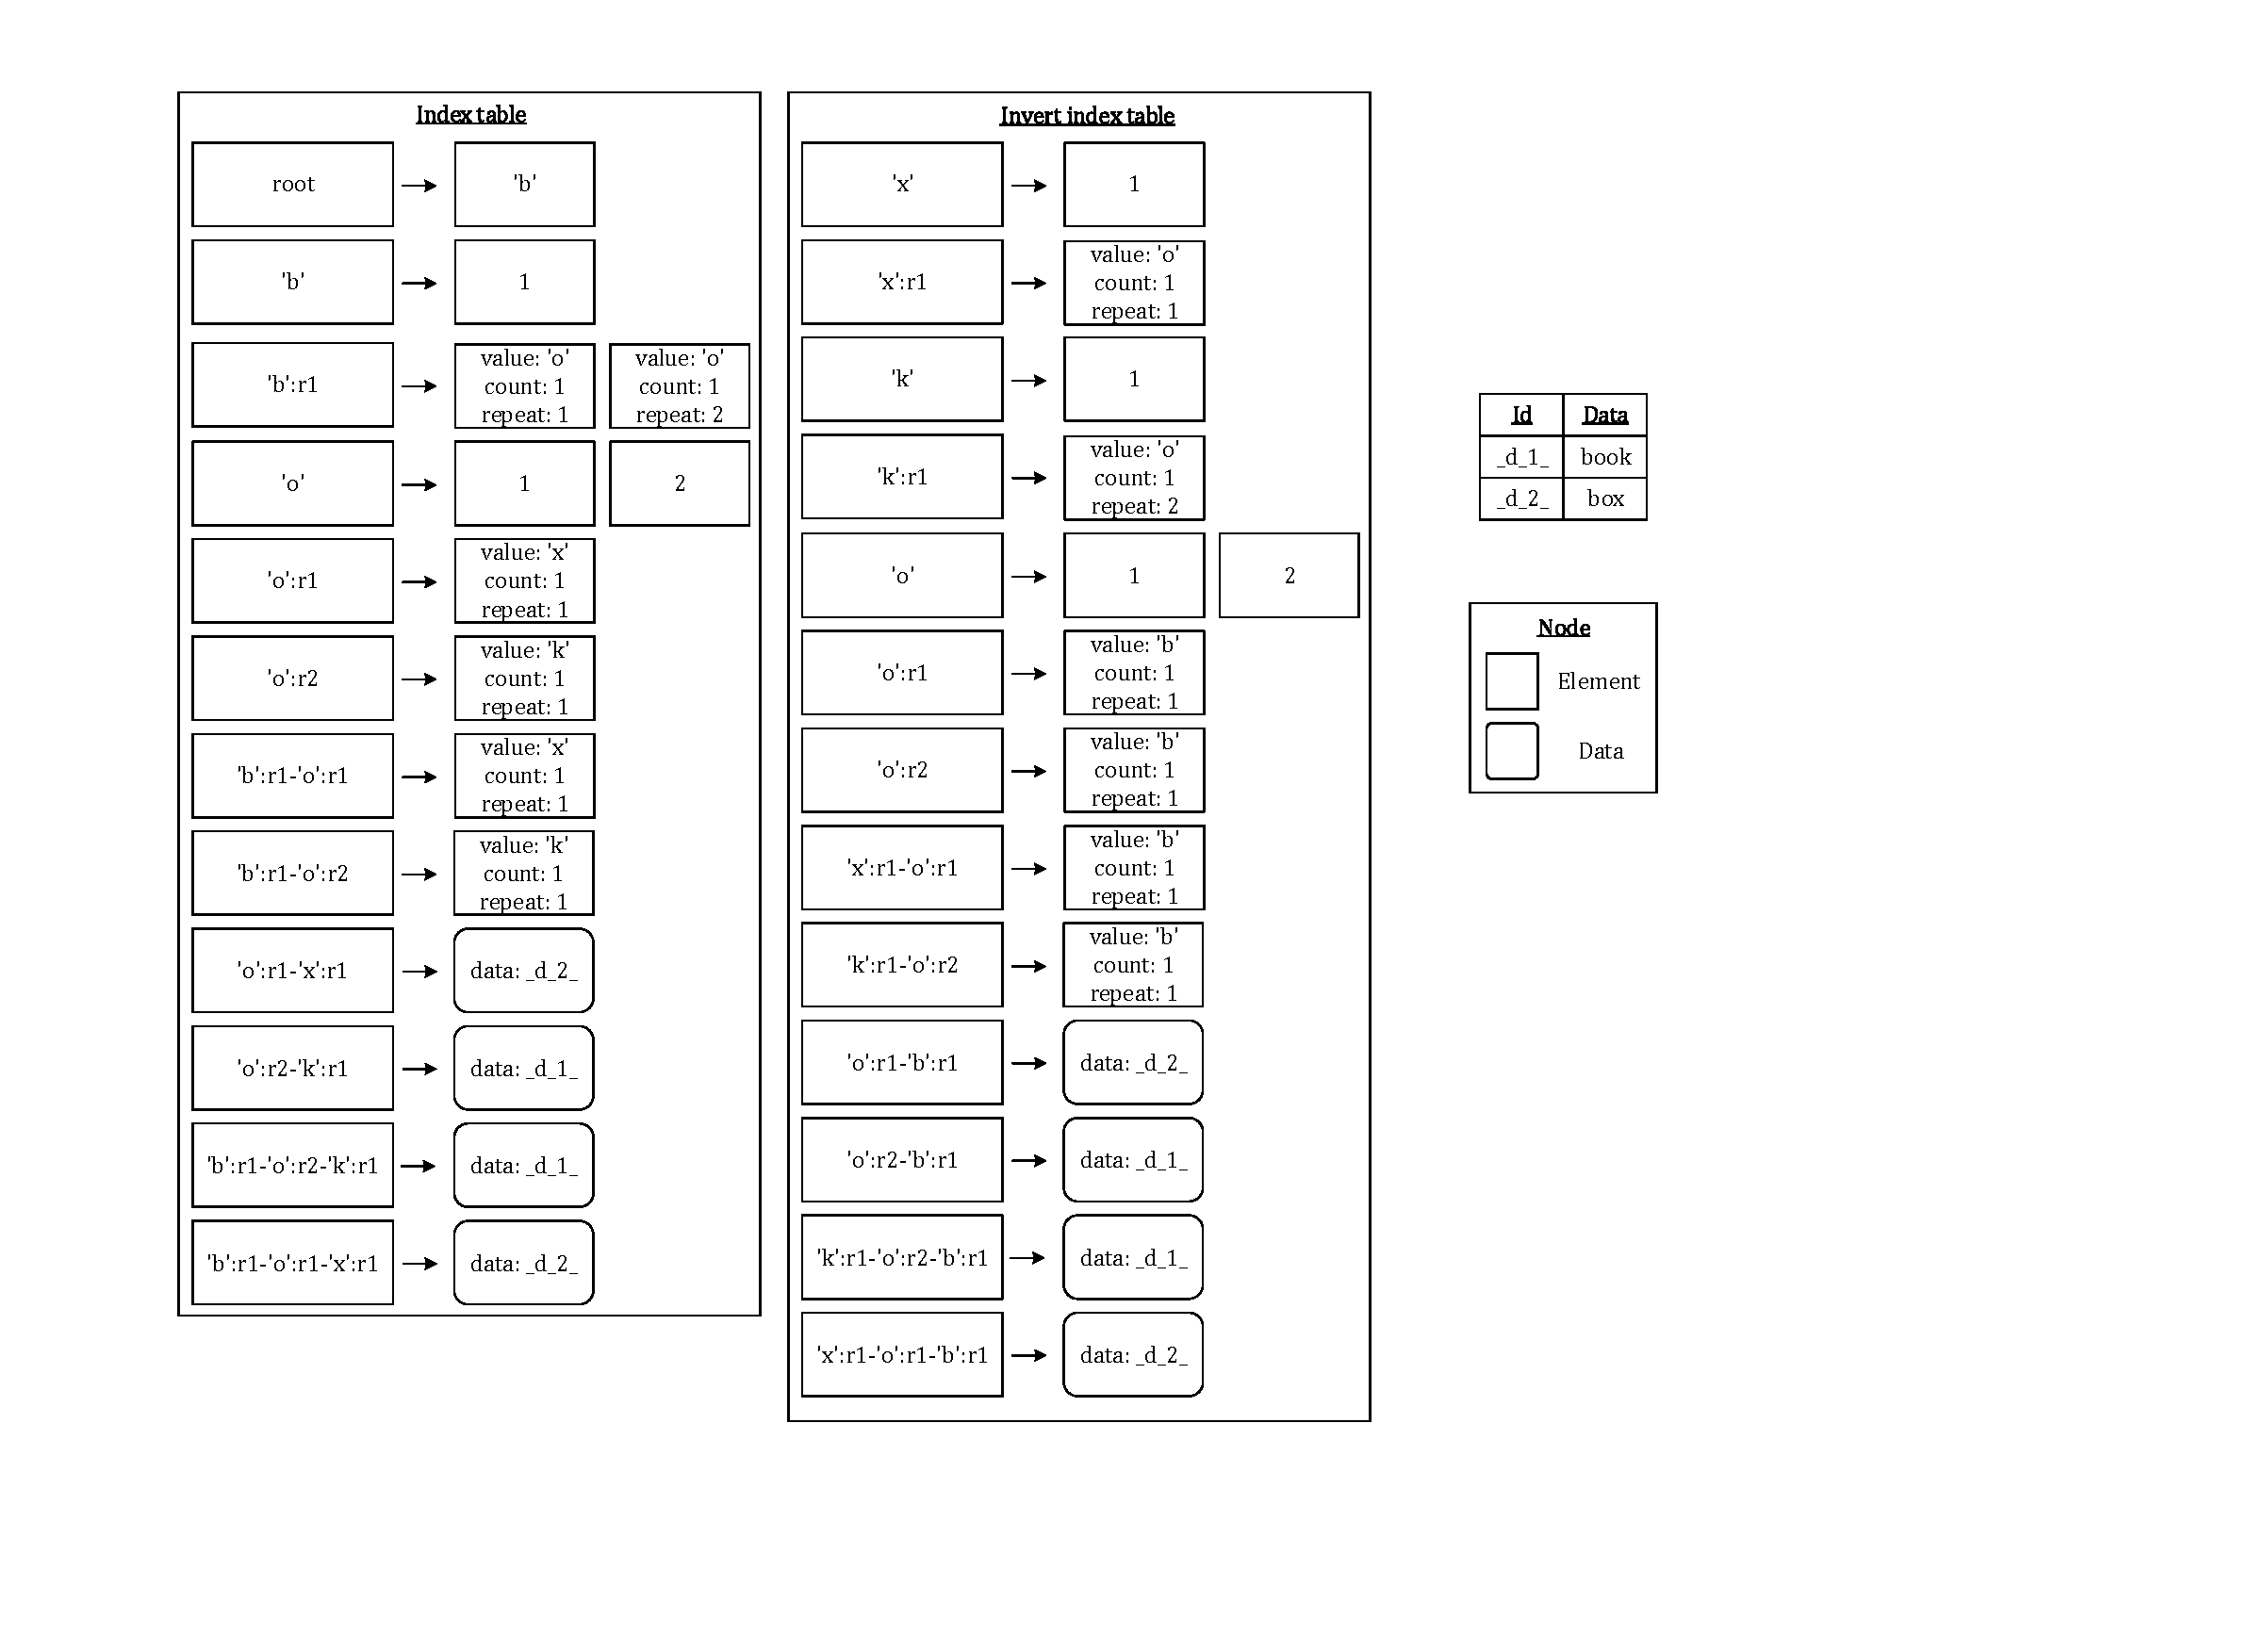
\includegraphics[scale=0.6]{./algorithm/string/pic/insertion/example_2_v5.pdf}
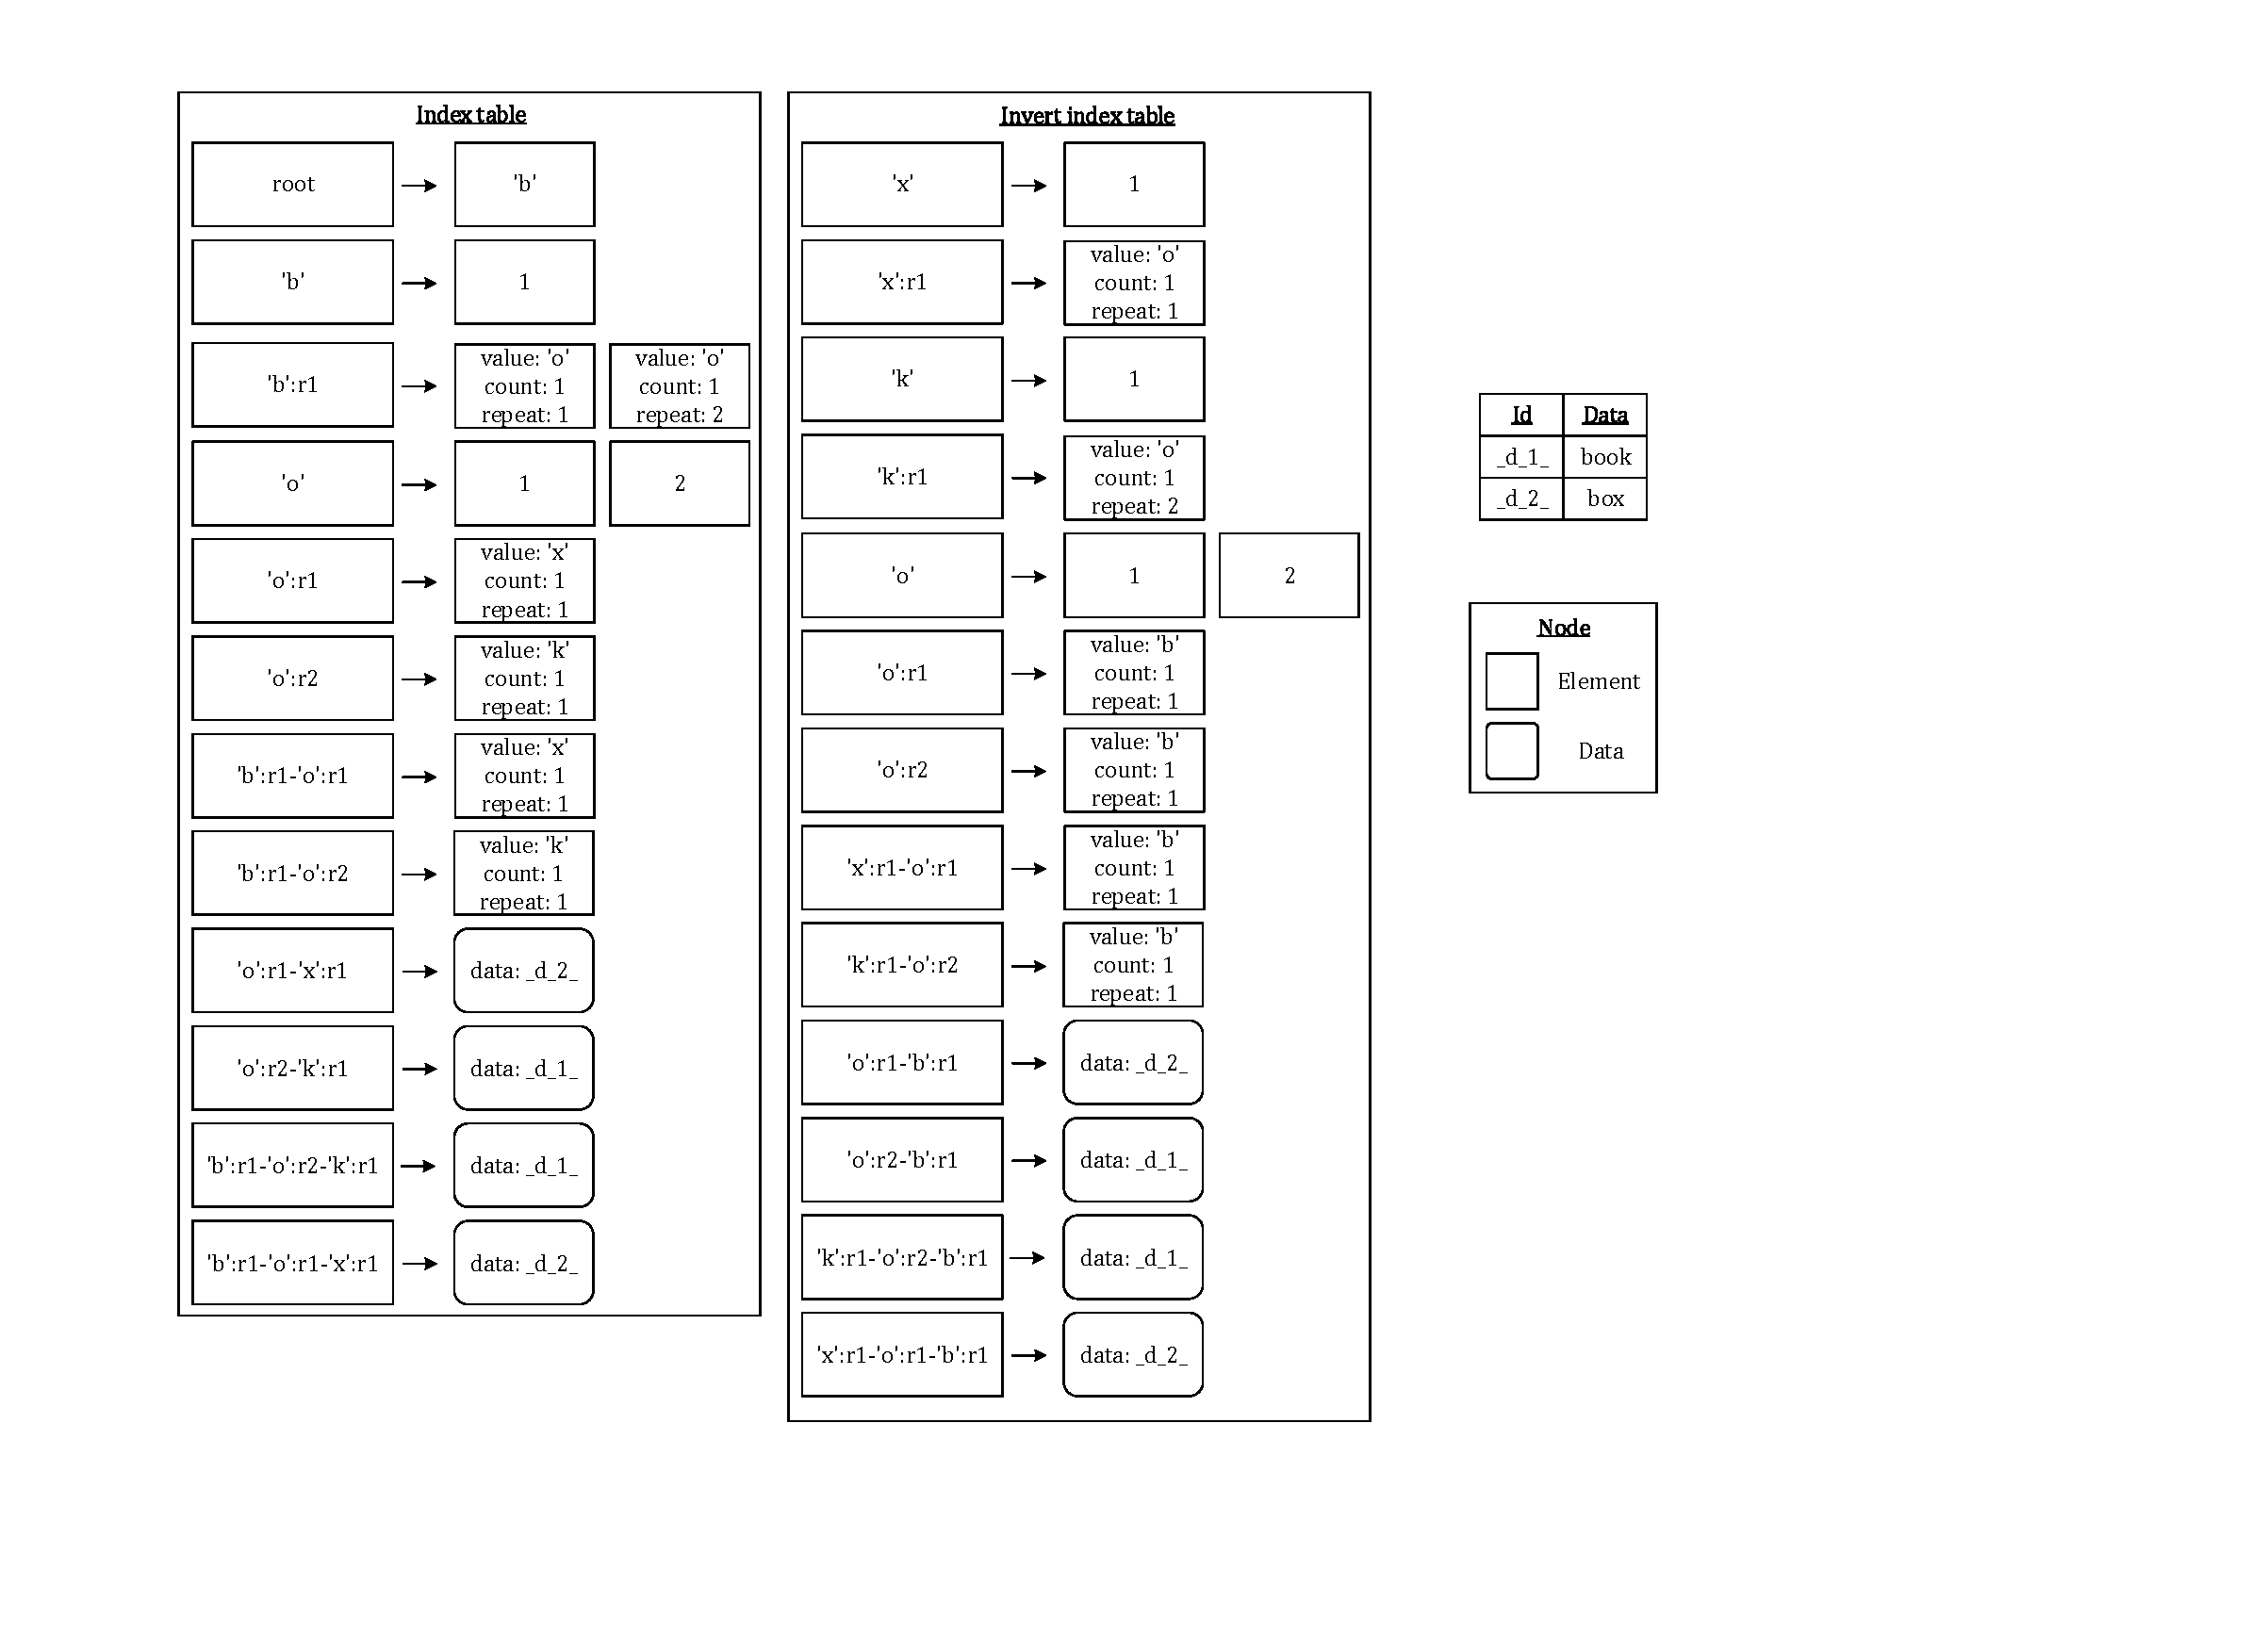
\includegraphics[width=0.8\textwidth]{./algorithm/string/pic/insertion/example_2_v5.pdf}
\caption{Insert data \textit{"box"}.}
\label{fig:algorithm:string:insertion:example_2}
\end{figure}



% Deletion section
\subsubsection{Deletion}

In deletion, if a data need to be delete, and the bucket is only contain one node or data, then this mapping will be delete, otherwise only the count in the node will minus one. Next, delete the n-gram indexing in all index table.\\

Using the same example in figure \ref{fig:algorithm:string:insertion:example_2}. If removing the $"book"$ which will remove some nodes in both index table, and then the tables should look like figure \ref{fig:algorithm:string:deletion:example_1}. For better understanding, the nodes which need to remove will use the line over it.

\begin{figure}[h]
\centering
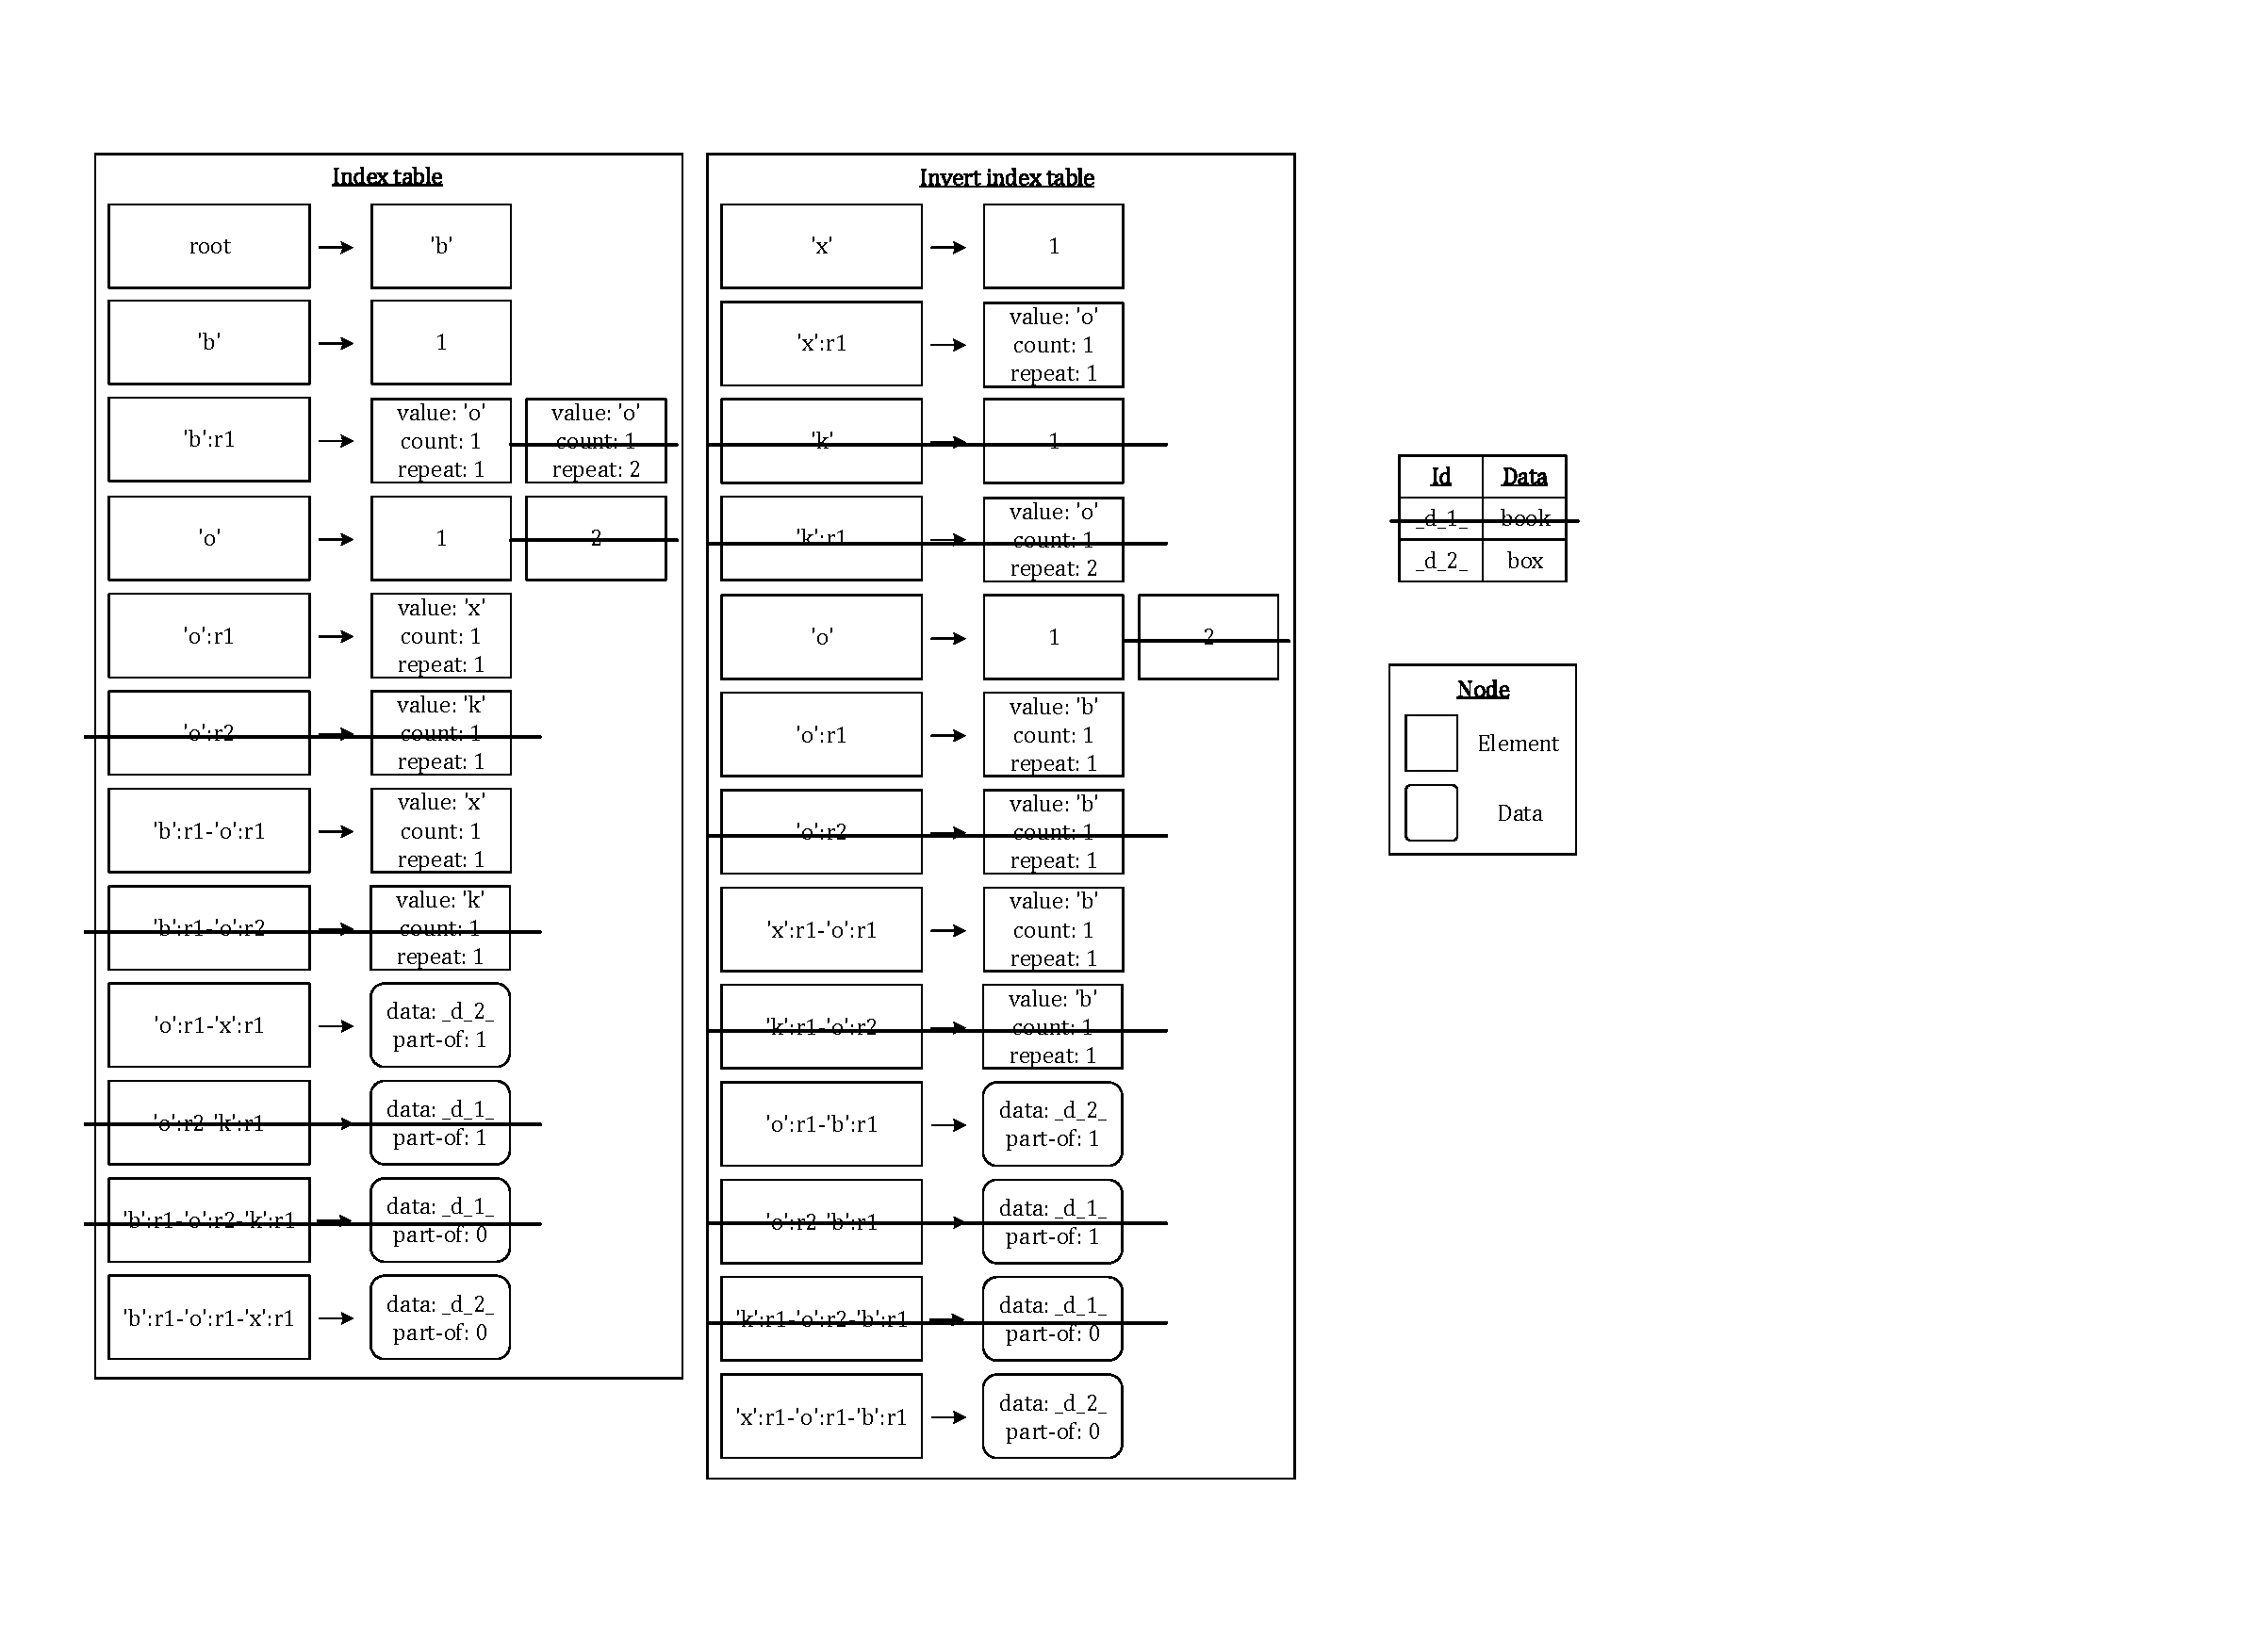
\includegraphics[scale=0.4]{./algorithm/string/pic/deletion/example_1_v3.pdf}
\caption{Delete $"book"$ from table.}
\label{fig:algorithm:string:deletion:example_1}
\end{figure}

The time needed is equals to $2 * O(b!)$, $b$ is the number of for loop which is equal to the byte length of string in one table (Normally it is equal, but in this case $(b = 3)$ which is because the $"o"$ have handled by the repeat counting). Because $2 * O(b!)$ is domain as $O(b)$, so the time complexity of delectation is $O(b)$.



% Modification section
\subsubsection{Modification}

Modify a data, actually is combining insert and delete, but without modified the data $id$. So the time complexity is $2 * O(b)$ operation but domain as $O(b)$.


% Selection section
\subsubsection{Selection}

The selection is the main core of Li's Hash, because the purposes of the index tables is to design for high-speed searching operation which means the Li's Hash can do the searching operation for key-value store.

Using the same example of figure \ref{fig:algorithm:string:insertion:example_2} from insertion section.

% Operation
\begin{enumerate}

% --------------------------------------------------------

\item \textbf{Exact matching}

As normal key-value store, if searching the data as \textit{"book"}, which convert into the key as \textit{"'b':r1-'o':r2-'k':r1"} and search in index table, and return the result of data node \textit{"\_d\_1\_"} in $O(1)$.

% --------------------------------------------------------

\item \textbf{Prefix matching}

If searching \textit{"bo"} as prefix which as same as \textit{"LIKE 'bo\%'"} in SQL. Using the key as \textit{"'b':r1"} from index table, will get the metadata that can know the next keys \textit{"'b':r1$-$'o':r1"} and \textit{"'b':r1$-$'o':r2"}. So fellow these two keys will get \textit{"'b':r1-'o':r1-'x':r1"} and \textit{"'b':r1-'o':r2-'k':r1"}, and using this two keys will get the data node \textit{"\_d\_1\_"} and \textit{"\_d\_2\_"}.

So the concept of search is fellow the metadata if get an element node, and add the data into the return list if pointing to a data node. Repeat search in table with this way until there is no element node can fellow.

And the time complexity should be $O(b)$.

% --------------------------------------------------------

\item \textbf{Suffix matching}

Similar as prefix matching, the different is using inverted index table rather than index table. So if try to search \textit{'x'} as suffix which as same as \textit{"LIKE '\%x'"} in SQL, using the key \textit{'x'} and get \textit{"'x':r1"} as return, and the remain is as same as the searching in prefix matching which will get the data node \textit{"\_d\_2\_"} in final. The time complexity is $O(b)$.

% --------------------------------------------------------

\item \textbf{Partial matching}

Partial matching is combining the prefix and suffix matching. For example if search \textit{'o'} for result which as same as using \textit{"LIKE '\%o\%'"} in SQL, then reassign as \textit{'o'} for prefix matching (\textit{"LIKE 'o\%'"} in SQL) and suffix matching (\textit{"LIKE '\%o'"} in SQL), and the last step is to do intersection to both result.

The reason of existing the special keys is to record the repeat time like\textit{'o'-\textgreater1} or \textit{2}, or some keys like \textit{"'o':r1}-\textit{'x':r1"} which are target on this operation.

If these keys are not created, the search like above wouldn't be searchable because the \textit{'o'} is middle of the keys, it can't be found unless there is some query function provided by non-relational database where are  range scan or full scan, but we have already mentioned before.

And the time complexity should be $O(b) + O(b)$ that domain as $O(b)$.

% --------------------------------------------------------

\item \textbf{Retrieve all}

Using the key of \textit{"root"} in index table will get all the prefix byte of all result, this can simple retrieve all data in the database which the time complexity be $O(b)$.

% --------------------------------------------------------

\end{enumerate}


% Summary section
\subsubsection{Summary}

Table \ref{table:algorithm:string:summary:time_complexity} is the summary the time complexity of each opration in \textit{STRING} type.

\begin{table}[h]
\centering
\caption{Time complexity for \textit{STRING} type.}
\label{table:algorithm:string:summary:time_complexity}
\begin{tabular}{|c|c|}

\hline
\multicolumn{1}{|c|}{Operation} &
\multicolumn{1}{c|}{\tabincell{c}{
Time complexity \\ ($b$: The byte length of data)
}} \\

\hline
\multicolumn{1}{|c|}{Insert} &
\multicolumn{1}{c|}{$O(b)$} \\

\hline
\multicolumn{1}{|c|}{Modify} &
\multicolumn{1}{c|}{$O(b)$} \\

\hline
\multicolumn{1}{|c|}{Delete} &
\multicolumn{1}{c|}{$O(b)$} \\

\hline
\multicolumn{1}{|c|}{\tabincell{c}{
Search \\ (Exact matching)
}} &
\multicolumn{1}{c|}{$O(1)$} \\

\hline
\multicolumn{1}{|c|}{\tabincell{c}{
Search \\ (Prefix matching)
}} &
\multicolumn{1}{c|}{$O(b)$} \\

\hline
\multicolumn{1}{|c|}{\tabincell{c}{
Search \\ (Suffix matching)
}} &
\multicolumn{1}{c|}{$O(b)$} \\

\hline
\multicolumn{1}{|c|}{\tabincell{c}{
Search \\ (Partial matching)
}} &
\multicolumn{1}{c|}{$O(b)$} \\

\hline
\multicolumn{1}{|c|}
{\tabincell{c}{
Search \\ (Retrieve all)
}} &
\multicolumn{1}{c|}
{\tabincell{c}{
$O(b)$ \\ ($b$ is the longest string of all data)
}} \\

\hline
\end{tabular}
\end{table}


\clearpage


% BOOLEAN section
\subsection{BOOLEAN type}

The indexing in \textit{BOOLEAN} type is the simplest than other type, the invert index table is not needed because it is useless by doing the invert indexing just one single byte. So the table can be simplify as figure \ref{fig:algorithm:boolean:example_1}.

\begin{figure}[ht]
\centering
%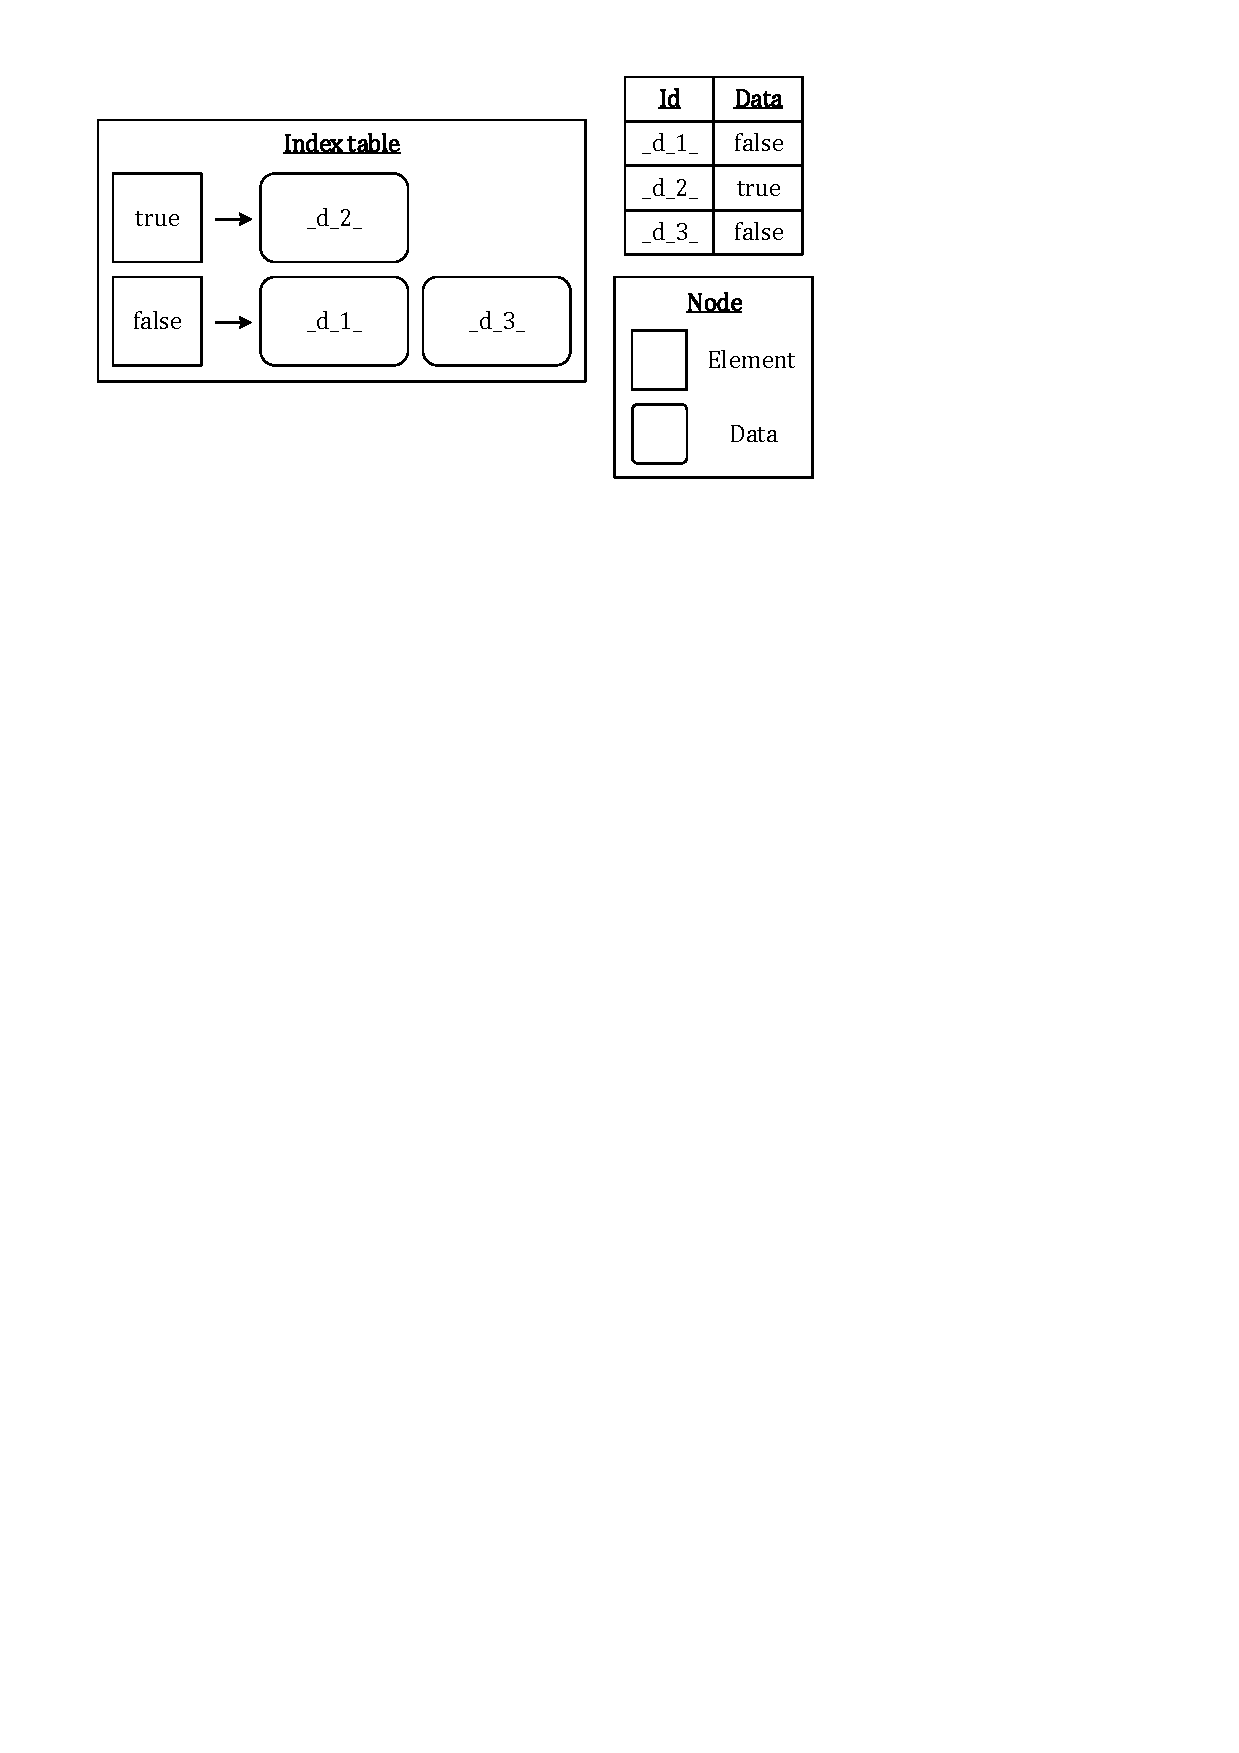
\includegraphics[scale=0.8]{./algorithm/boolean/pic/example_1_v1.pdf}
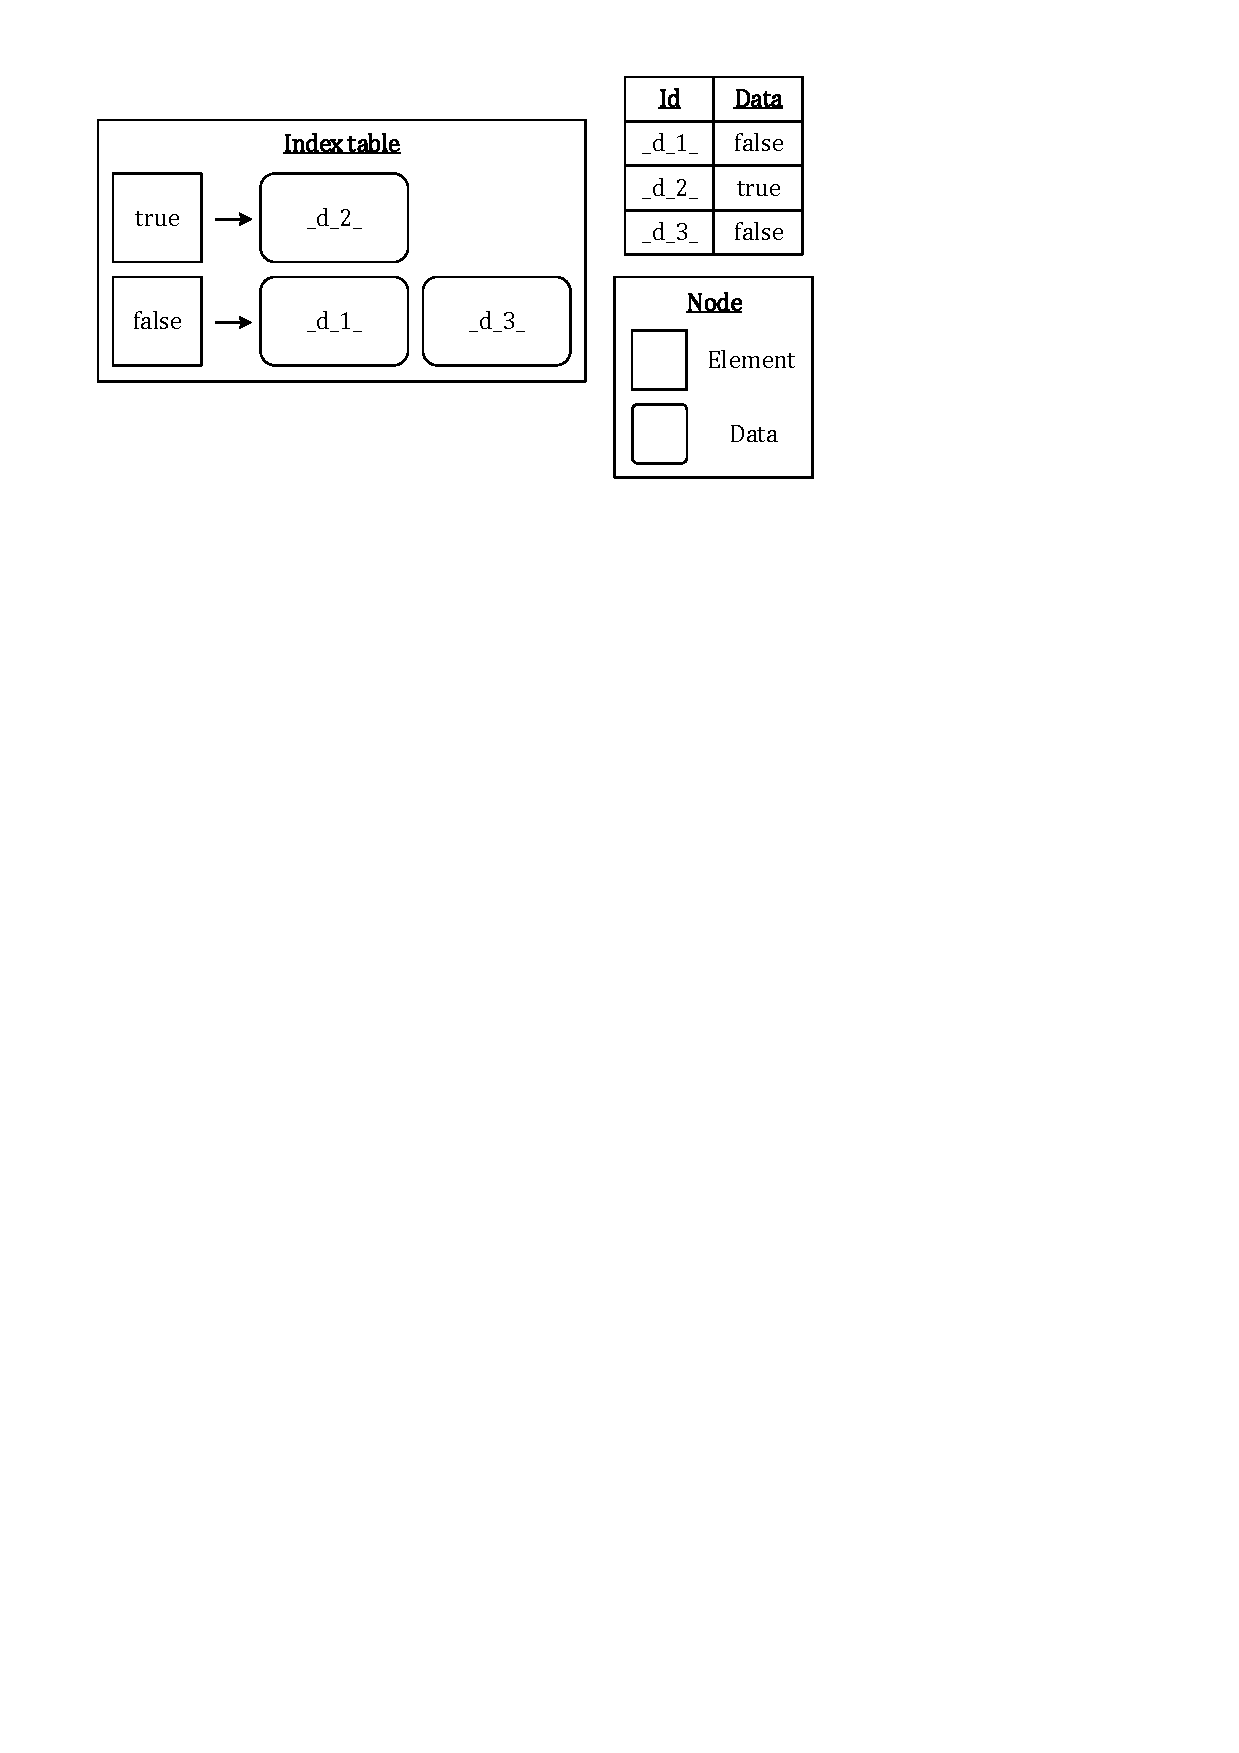
\includegraphics[width=0.8\textwidth]{./algorithm/boolean/pic/example_1_v1.pdf}
\caption{The indexing tables of in \textit{BOOLEAN} type.}
\label{fig:algorithm:boolean:example_1}
\end{figure}


% Insertion section
\subsubsection{Insertion}

When inserting a new data, it just need to add the data node into the bucket where the data belong with, so the time complexity should be $O(1)$.


% Deletion section
\subsubsection{Deletion}

Delete a data node is just get the bucket and remove the data node, so this is also a quick operation where time complexity be $O(1)$.


% Modification section
\subsubsection{Modification}

Modify the data is actually delete the node in a bucket and re-insert it again into another bucket. Time complexity should be $O(1)$.



% Selection section
\subsubsection{Selection}

Select operation is the simplest operation than the other, because the selection for \textit{BOOLEAN} type is only can select $"true"$ or $"false"$, so select the bucket then this will return the whole bucket, so this is also a quick operation. Also if user want to retrieve all, just retrieve both $"true"$ and $"false"$ bucket will get all data. That time complexity of both searching are $O(1)$.


% Summary section
\subsubsection{Summary}

Table \ref{table:algorithm:boolean:summary:time_complexity} is summarized the time complexity of each opration in \textit{BOOLEAN} type.

\begin{table}[h]
\centering
\caption{Time complexity for \textit{BOOLEAN} type.}
\label{table:algorithm:boolean:summary:time_complexity}
\begin{tabular}{|c|c|}

\hline
\multicolumn{1}{|c|}{Operation} &
\multicolumn{1}{c|}{Time complexity} \\

\hline
\multicolumn{1}{|c|}{Insert} &
\multicolumn{1}{c|}{$O(1)$} \\

\hline
\multicolumn{1}{|c|}{Modify} &
\multicolumn{1}{c|}{$O(1)$} \\

\hline
\multicolumn{1}{|c|}{Delete} &
\multicolumn{1}{c|}{$O(1)$} \\

\hline
\multicolumn{1}{|c|}{Selection} &
\multicolumn{1}{c|}{$O(1)$} \\

\hline
\end{tabular}
\end{table}


\clearpage


% INTEGER section
\subsection{INTEGER type}

The \textit{INTEGER} type is design as 8 bytes $({b} = 8)$, but for easy to explain the \textit{INTEGER} type design in Li's Hash, so the example below which will explain in 4 bytes $(b = 4)$.\\

As normal integer, the \textit{INTEGER} type can be also signed and unsigned, this information will record in the metadata, so this will not show in index table, the different between them is the operation have a little bit different, but they share the same index table. Same as the \textit{BOOLEAN} type, the invert index table is not needed. Because of the inverted index table cost spaces but don't provide a significant speed up for the operation.\\

We use figure \ref{fig:algorithm:integer:example_1} to explain these operations below:

\begin{figure}[h]
\centering
%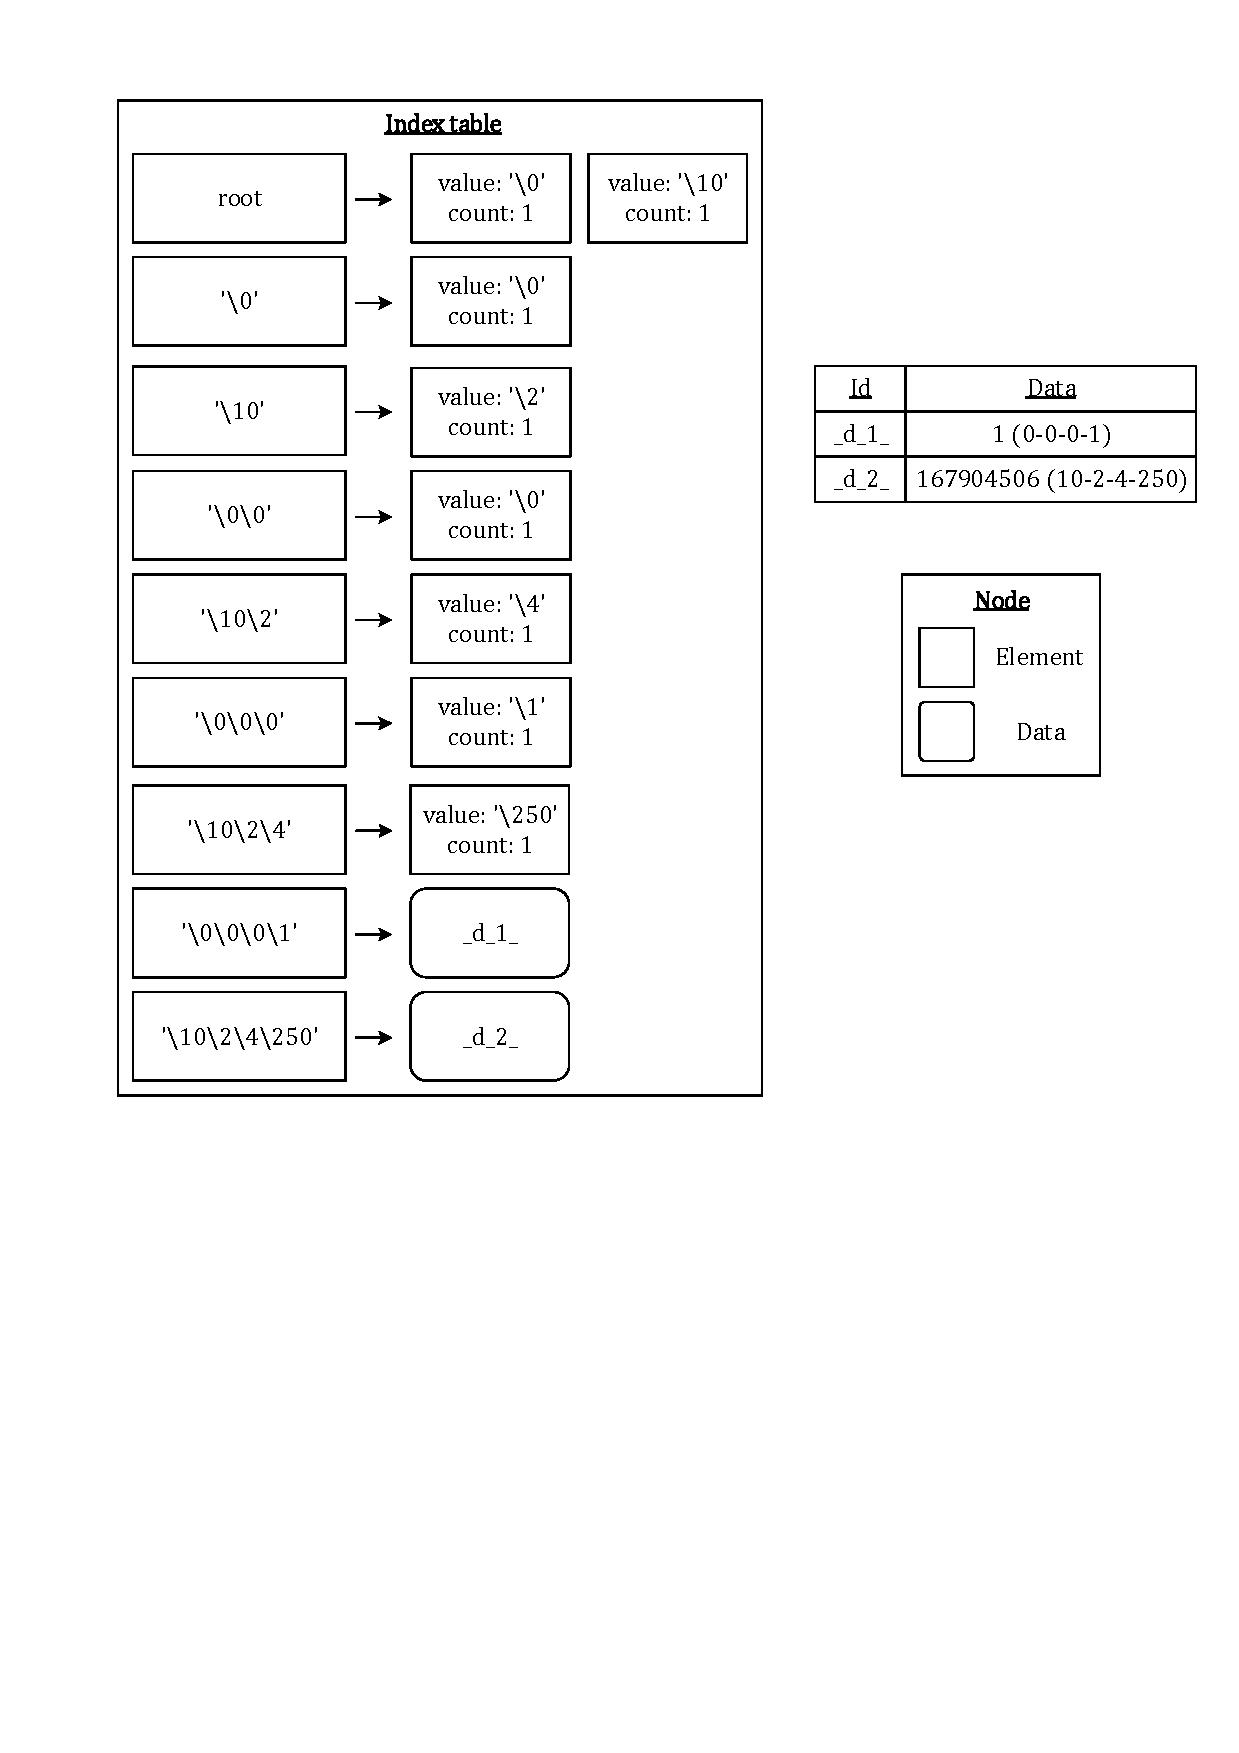
\includegraphics[scale=0.45]{./algorithm/integer/pic/example_1_v3.pdf}
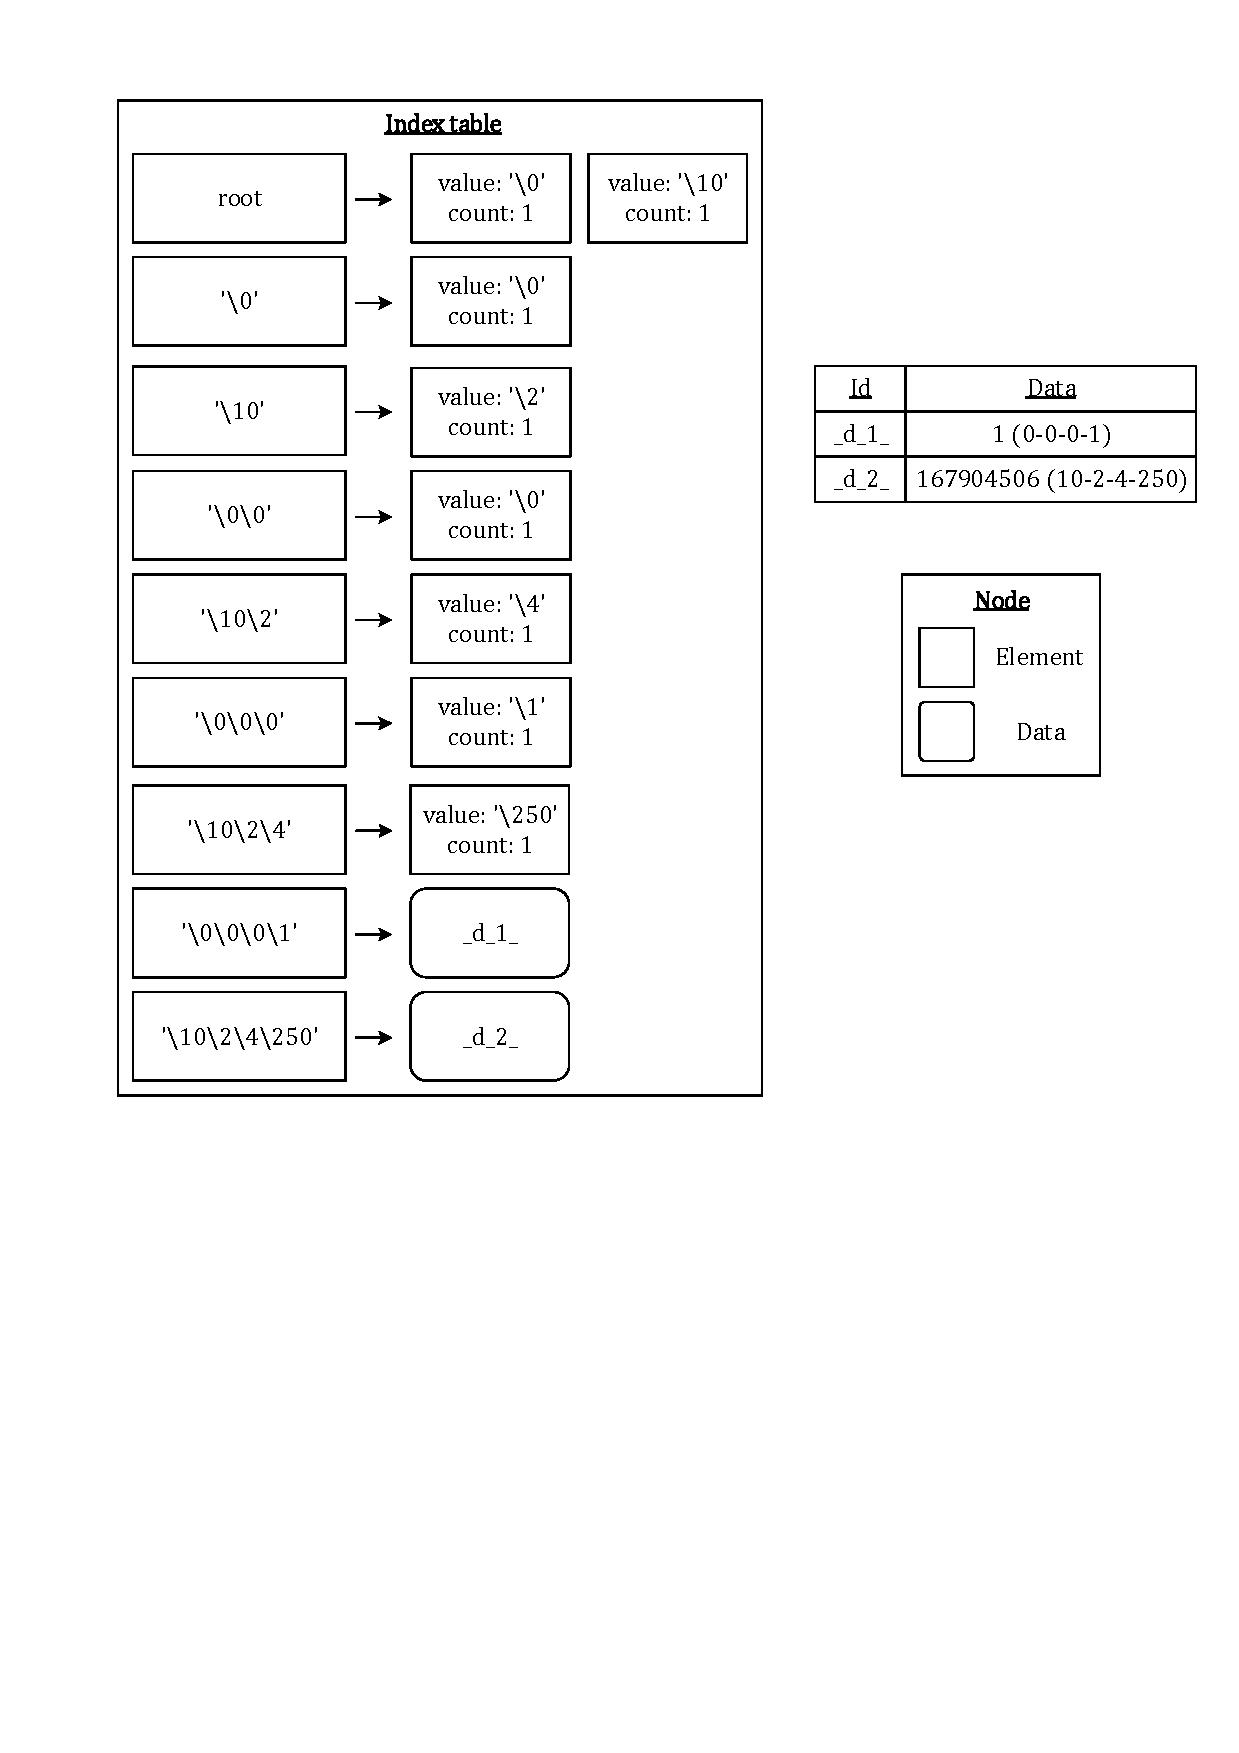
\includegraphics[width=0.8\textwidth]{./algorithm/integer/pic/example_1_v3.pdf}
\caption{The indexing tables of \textit{INTEGER} type.}
\label{fig:algorithm:integer:example_1}
\end{figure}

The index table is start with a root key \textit{'root'}. The root key is use to record the first byte of the data, so it will point to the range of 0 to 255.\\

In figure \ref{fig:algorithm:integer:example_1}, there are two data in the table. The four bytes of \textit{1} is \textit{0-0-0-1}, and \textit{167904506} is \textit{10-2-4-250} in byte. So in the table, the \textit{'root'} is pointing to \textit{'$\backslash0$'} and \textit{'$\backslash10$'}. After root key is finish its' indexing, the next step is just using n-gram indexing to index remain bytes to store data in the table.\\


% Insertion section
\subsubsection{Insertion}

Figure \ref{fig:algorithm:integer:example_1} already described some of the flow of insertion, so in here will show the table if insert a negative value into the table. Insert a -2147483647 (128-0-0-1) into table, which will become like figure \ref{fig:algorithm:integer:insertion:example_1}.

\begin{figure}[h]
\centering
%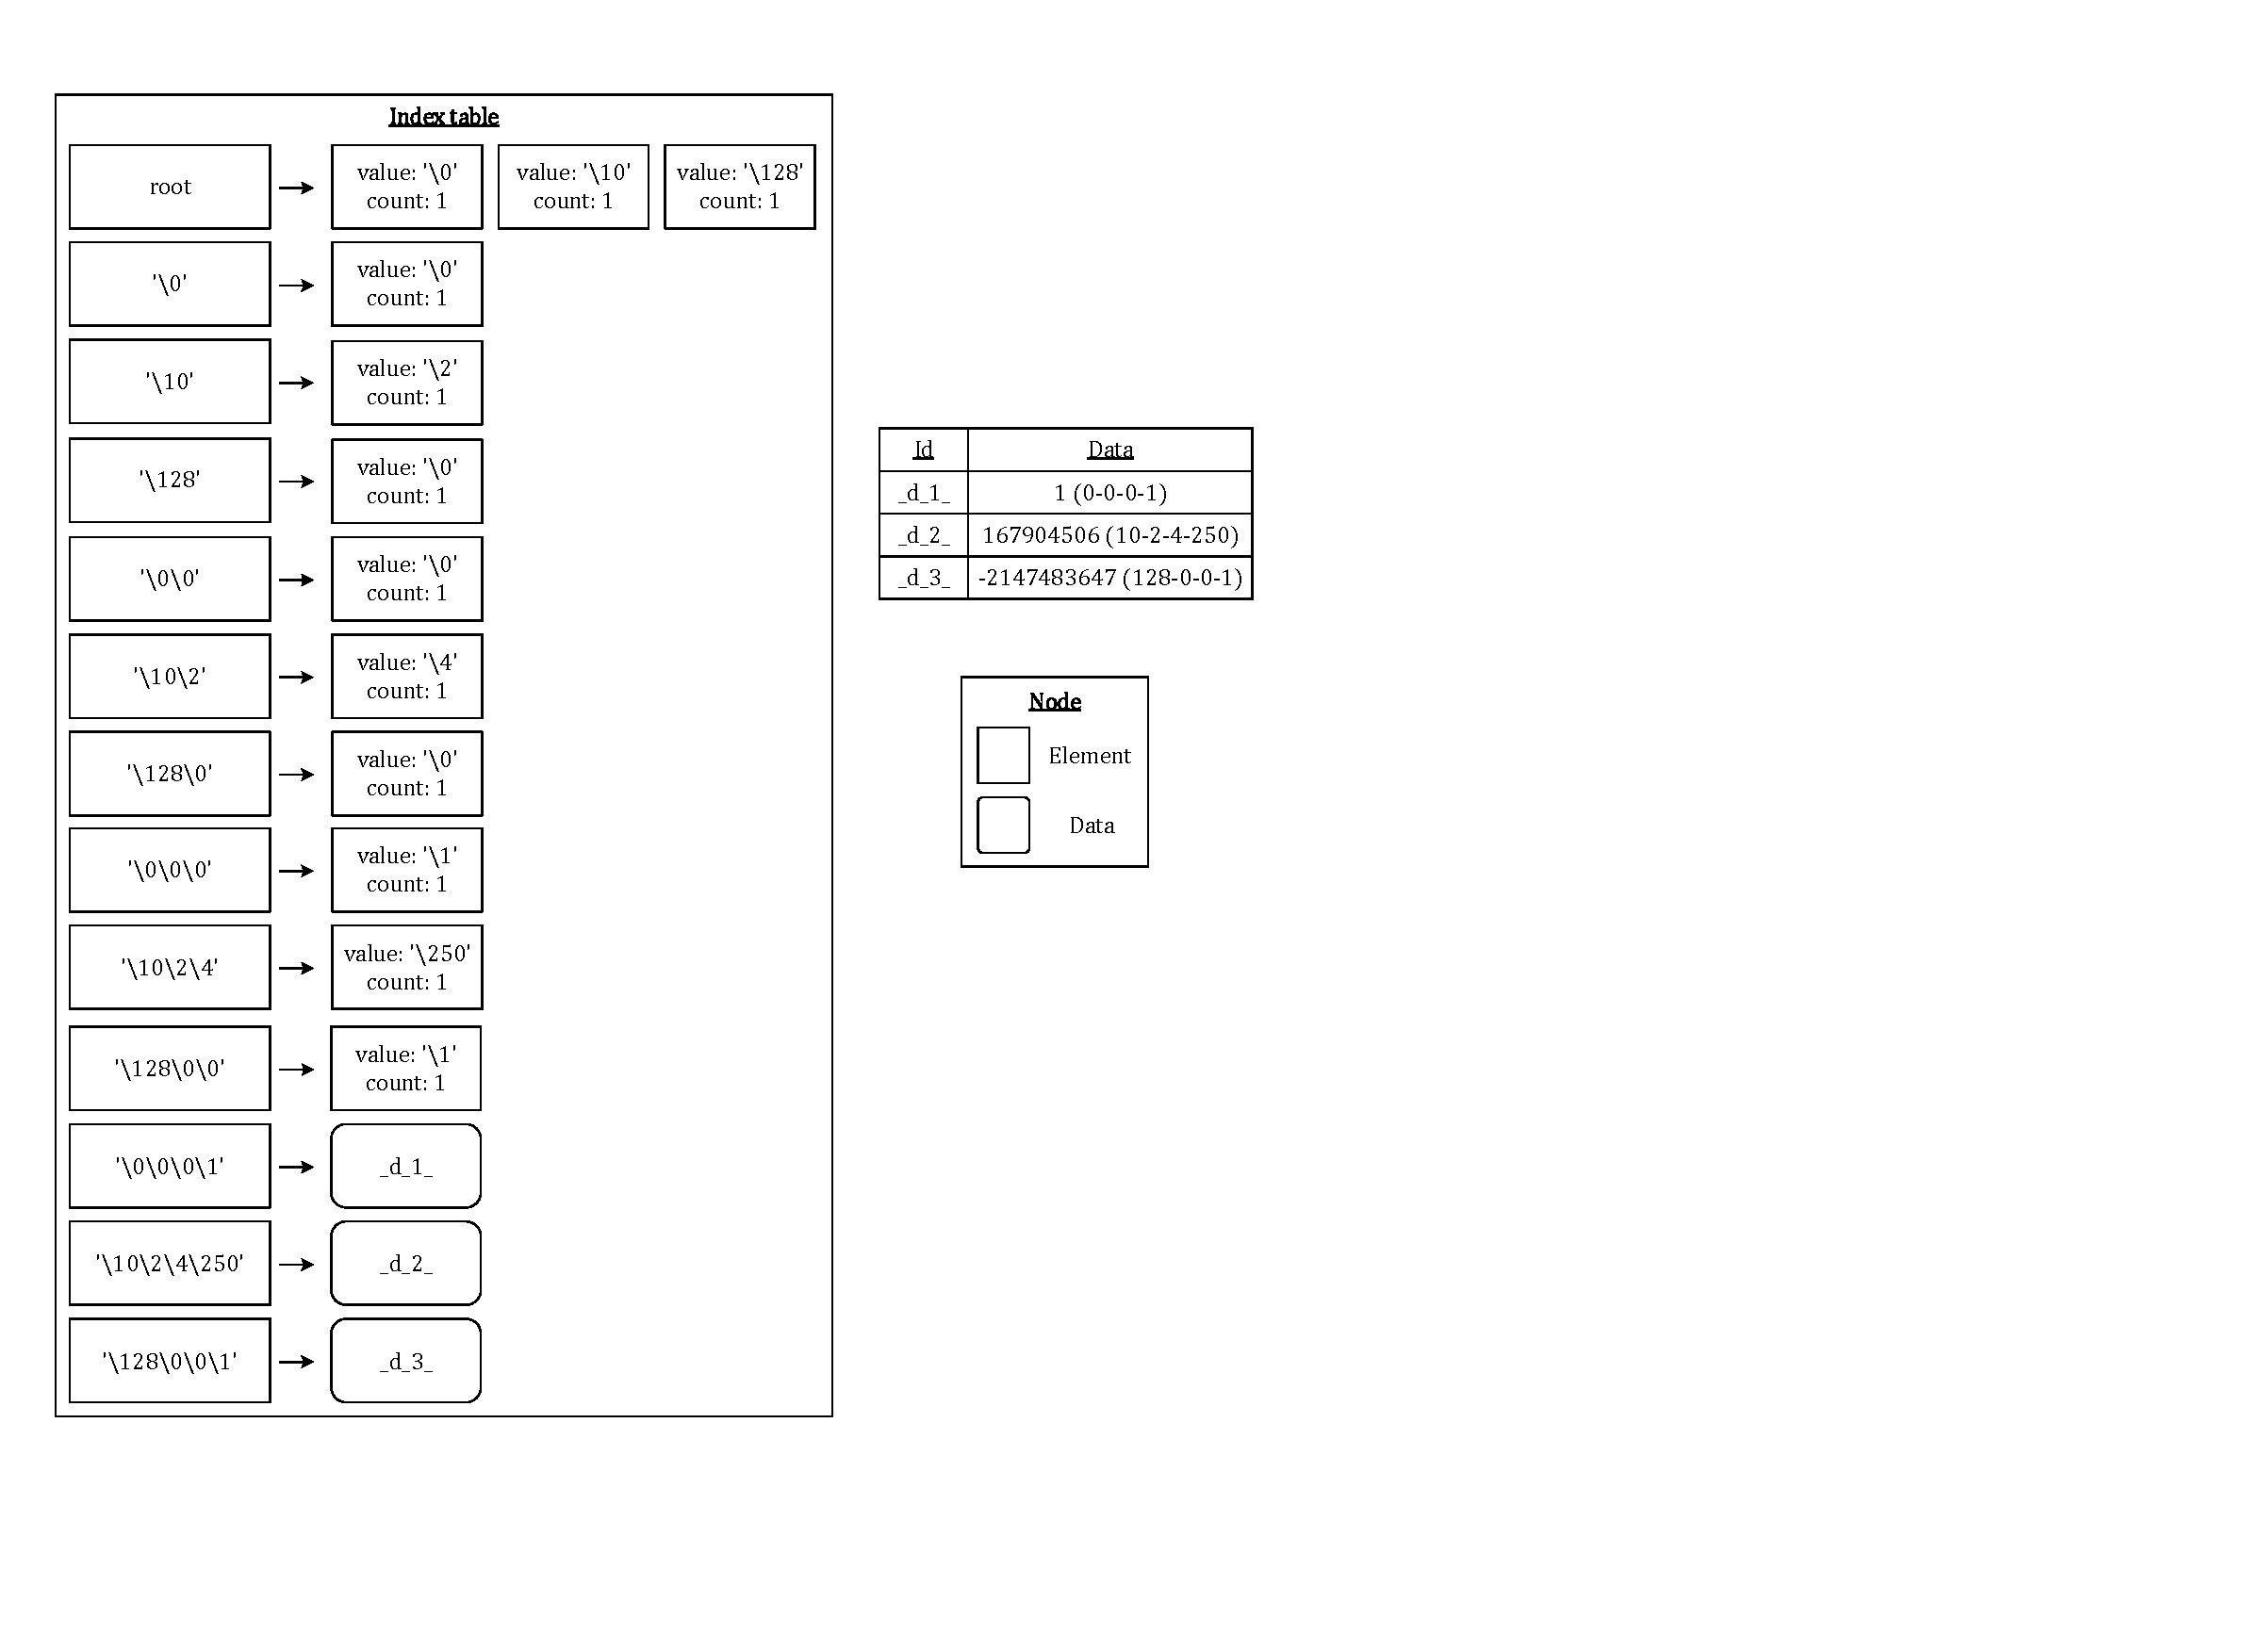
\includegraphics[scale=0.6]{./algorithm/integer/pic/insertion/example_1_v3.pdf}
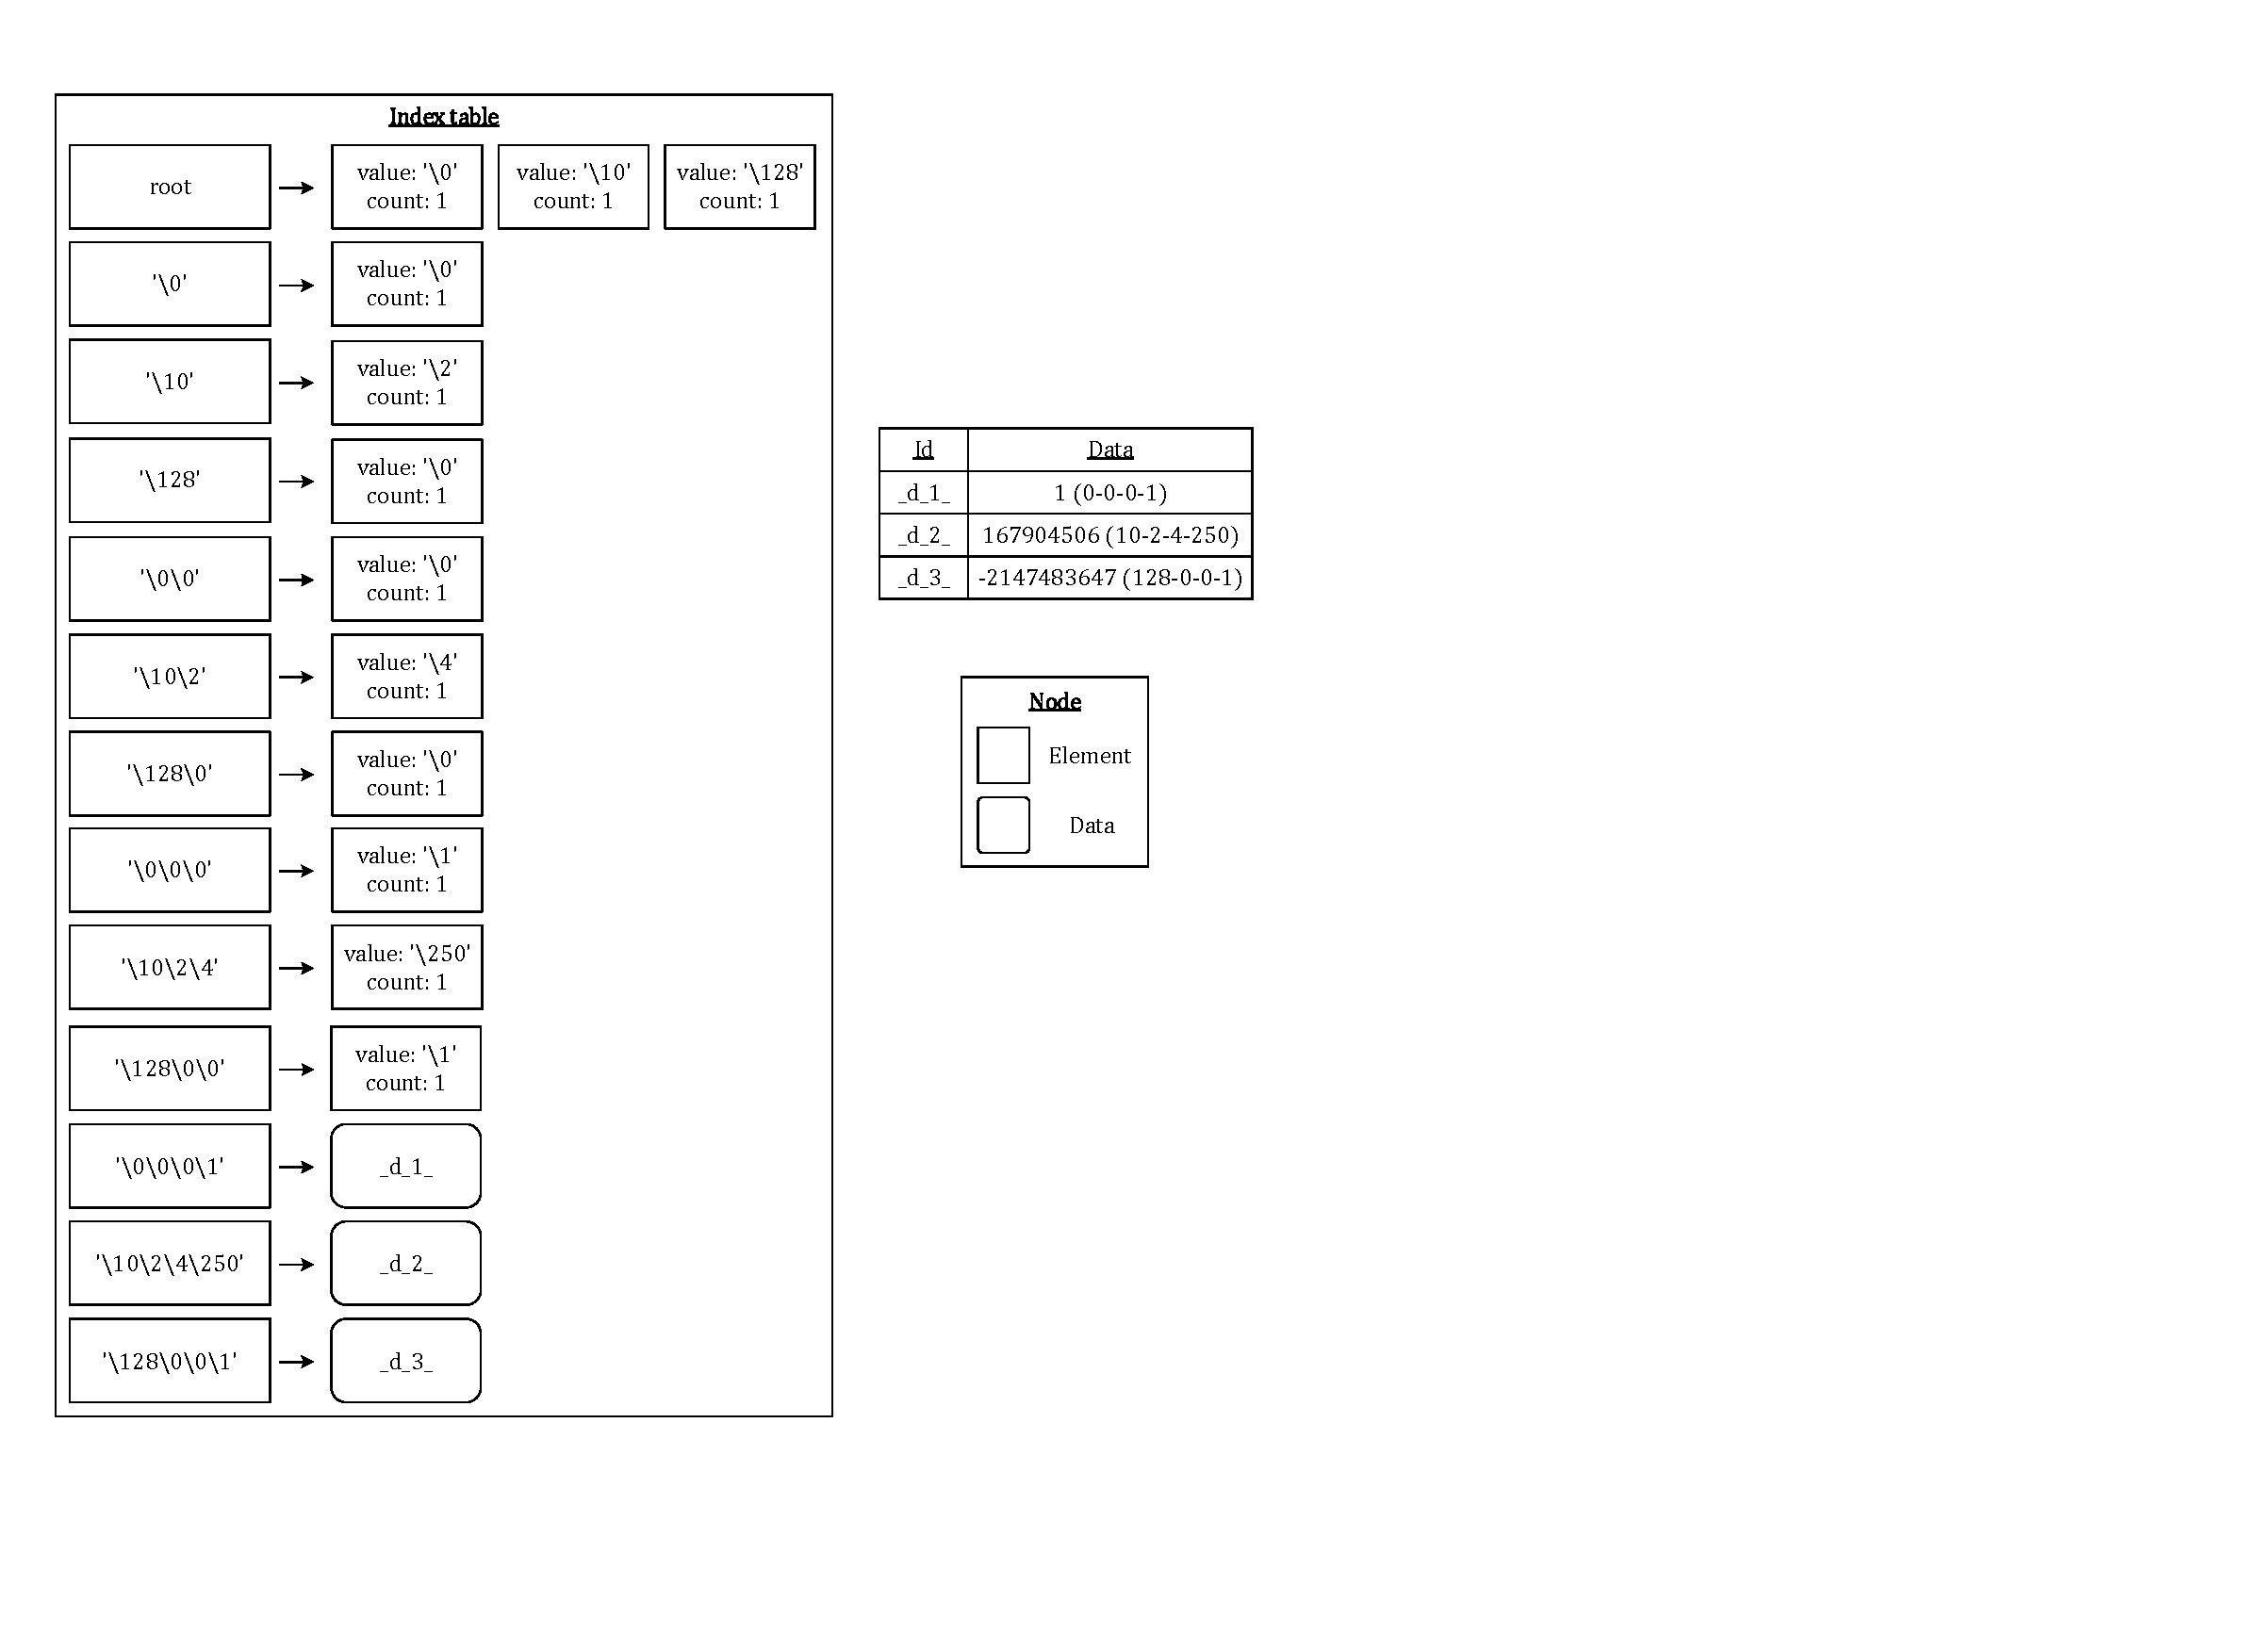
\includegraphics[width=0.8\textwidth]{./algorithm/integer/pic/insertion/example_1_v3.pdf}
\caption{The table after insert a negative value.}
\label{fig:algorithm:integer:insertion:example_1}
\end{figure}

Figure \ref{fig:algorithm:integer:insertion:example_1} shows that even a negative value will store as the same way as the positive value. And time complexity is $O(b)$.



% Deletion section
\subsubsection{Deletion}

Deletion is just do the opposite insertion to remove the byte and decrease the count. Fellow the same rule, if the count become zero, then the node will be remove. The time complexity is also $O(b)$.


% Modification section
\subsubsection{Modification}

The modify flow are similar as \textit{STRING} type, remove the key which don't needed and add the count if the byte is the same. So follow the example in figure \ref{fig:algorithm:integer:insertion:example_1} and modify 167904506 (10-2-4-250) to 2 (0-0-0-2), the table will look like figure \ref{fig:algorithm:integer:modification:example_1} and time complexity is $O(b)$.

\begin{figure}[h]
\centering
%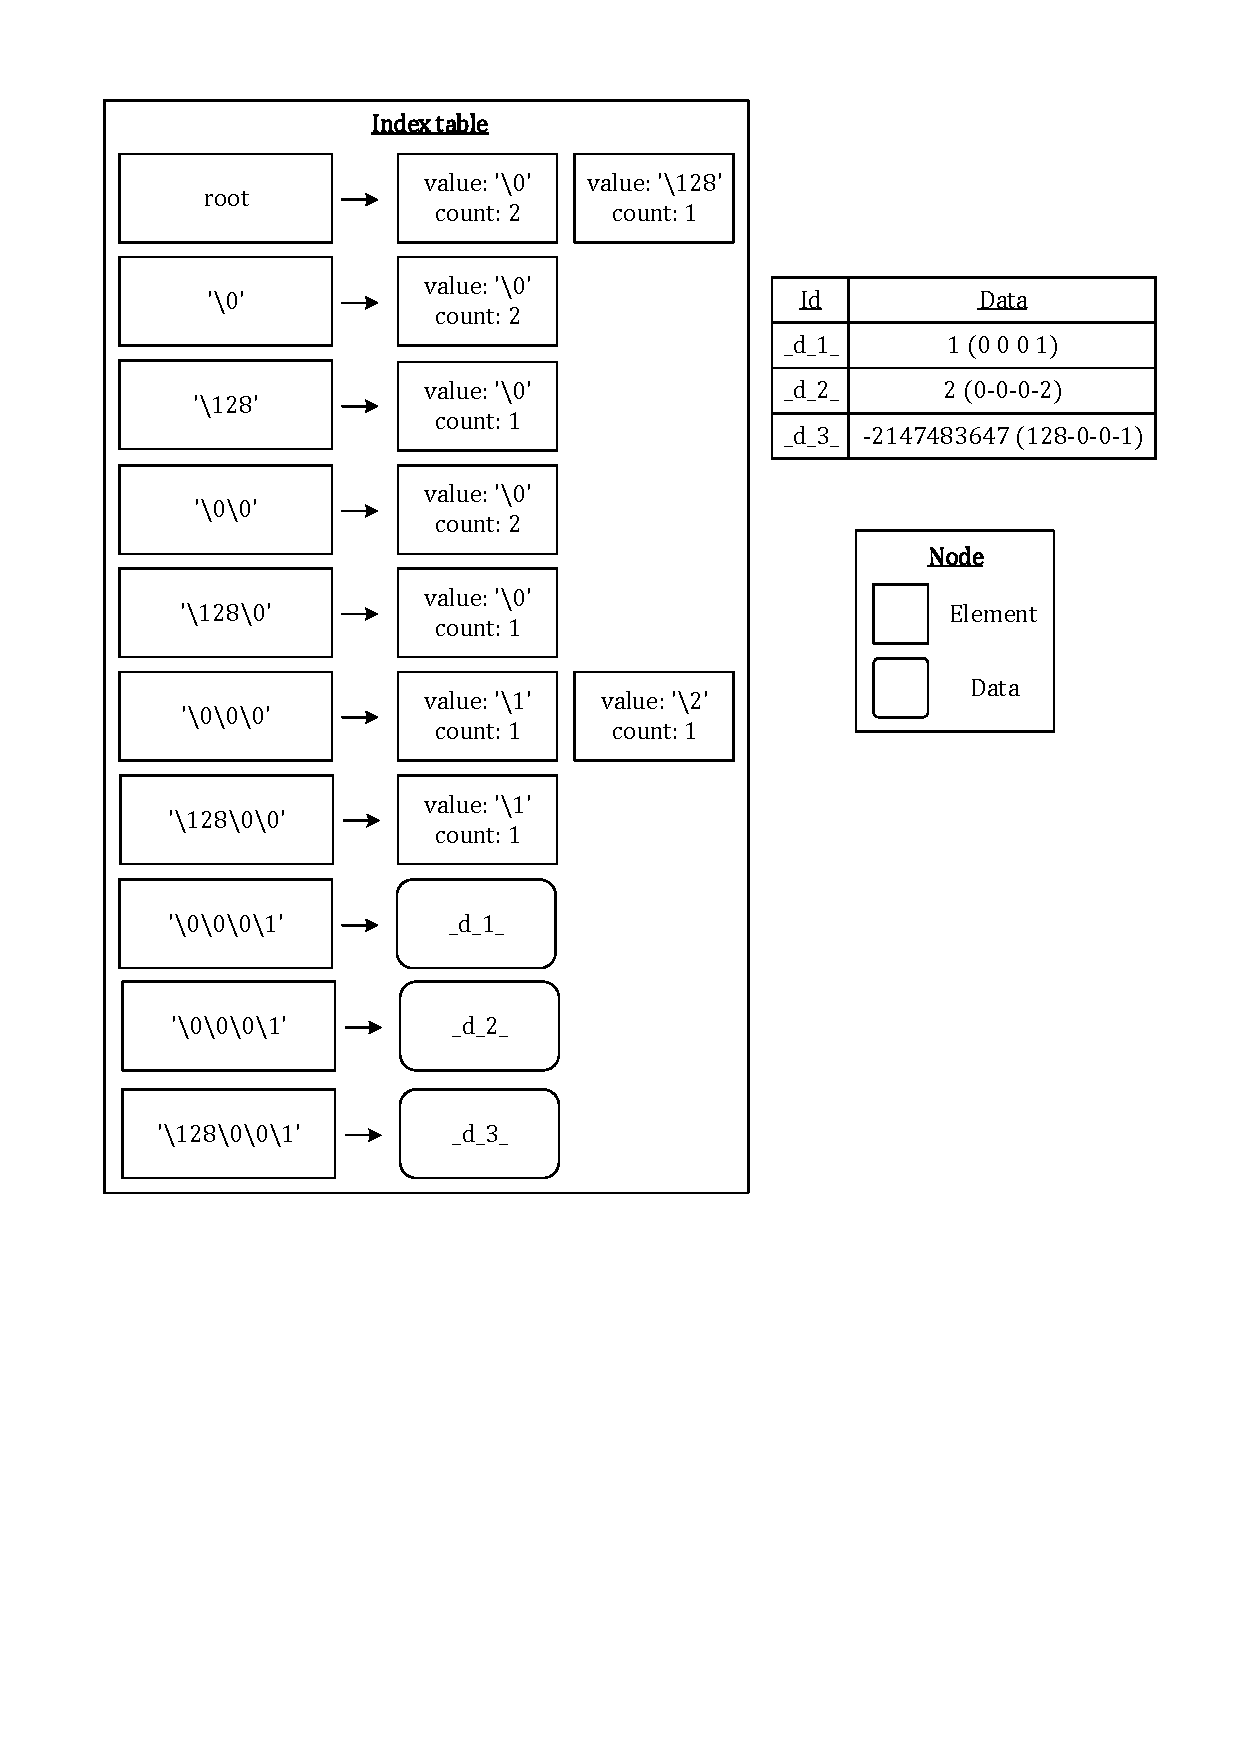
\includegraphics[scale=0.6]{./algorithm/integer/pic/modification/example_1_v3.pdf}
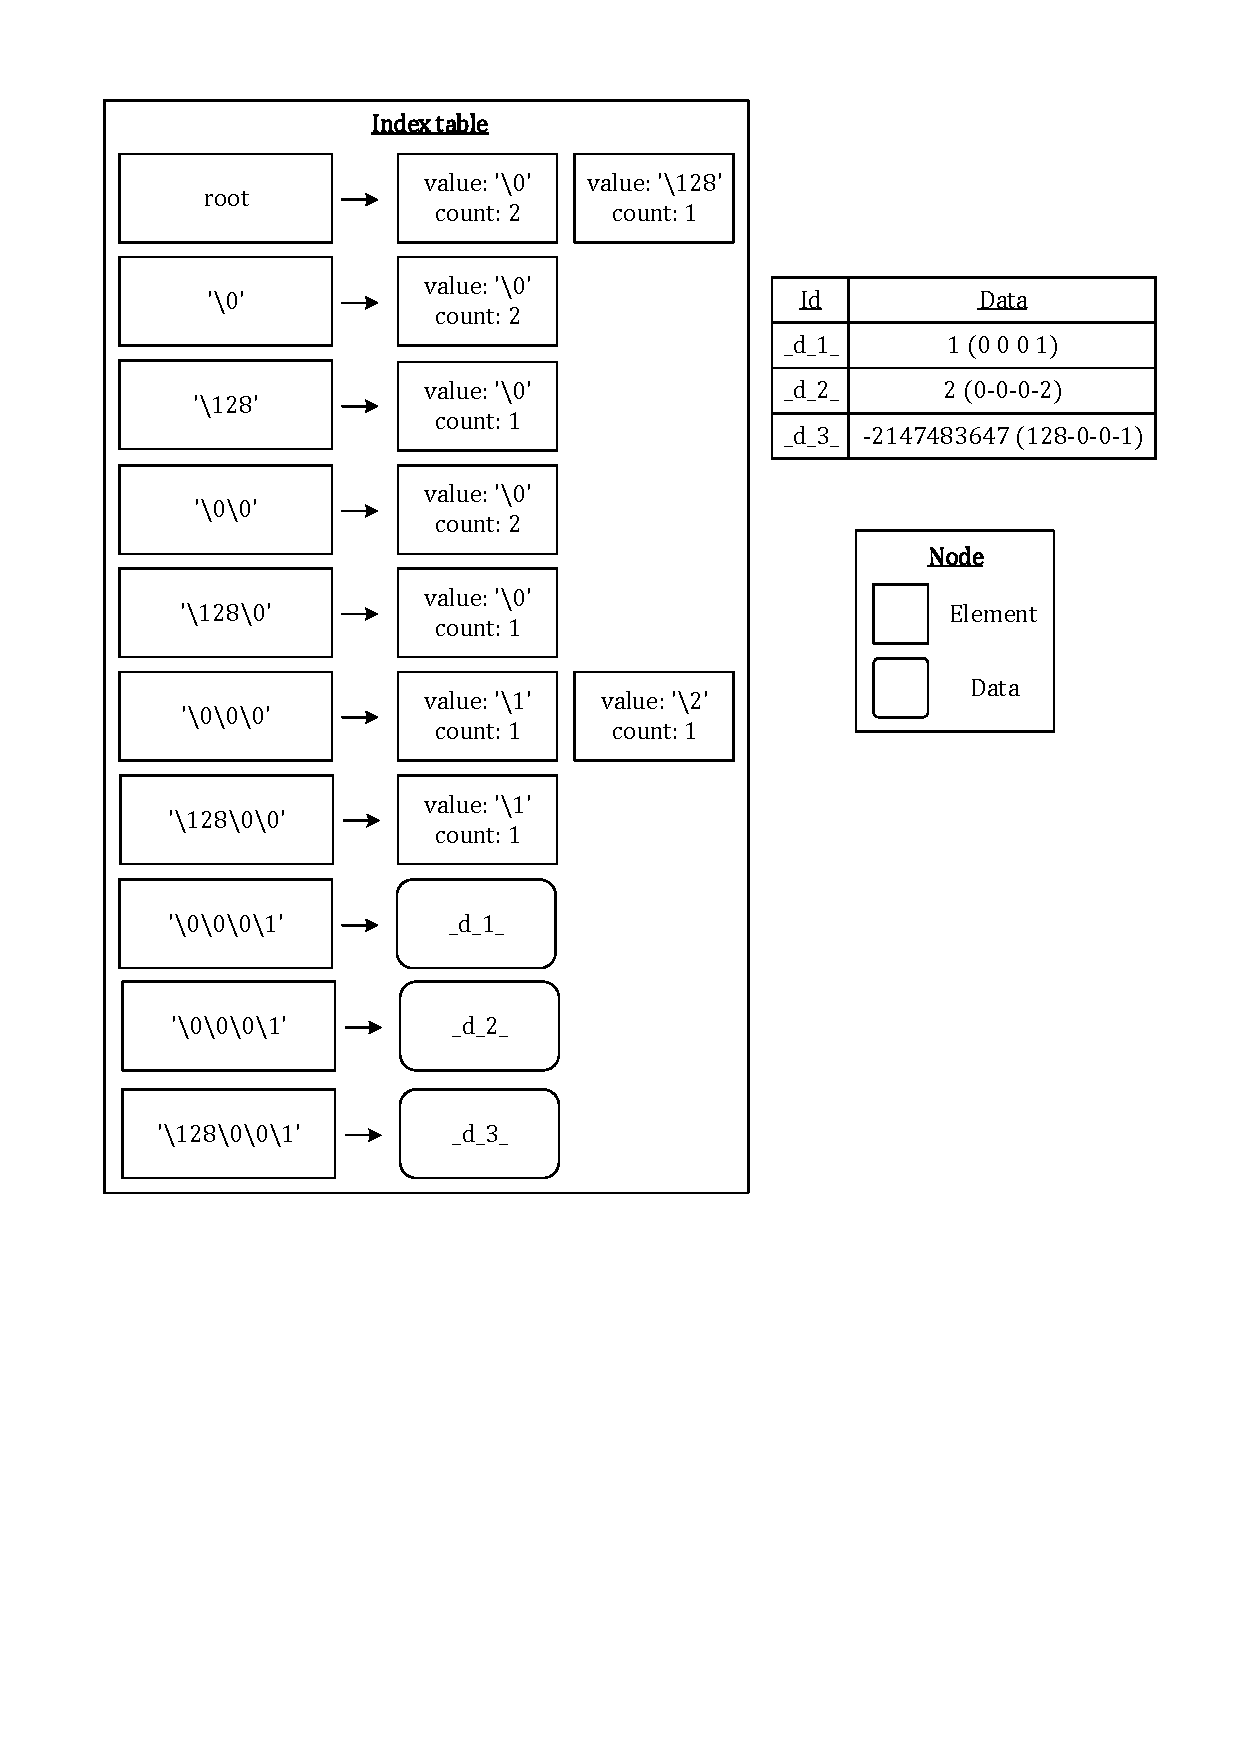
\includegraphics[width=0.8\textwidth]{./algorithm/integer/pic/modification/example_1_v3.pdf}
\caption{The table after modified the value.}
\label{fig:algorithm:integer:modification:example_1}
\end{figure}



% Selection section
\subsubsection{Selection}

Normally the database proves some function for compare the value of searching, so the Li's Hash musts also can do the same thing.

We use figure \ref{fig:algorithm:integer:modification:example_1} as example to demo the selection.

% Selection section enumerate
\begin{enumerate}

% --------------------------------------------------------

% Equal section
\item \textbf{Equal}

Compare the value is very simple. For example if we want to find data is equal to \textit{1 (0-0-0-1)}, we just need to use the key as $'\backslash0\backslash0\backslash0\backslash1'$ to search the index table. This should only take the time as $O(1)$.

% --------------------------------------------------------

% Not equal section
\item \textbf{Not equal}

Because it can't directly use the input value as key. So in this operation, it will start with the root key and parse all the result to find these element node until find the data node, but skip checking the key is as same as the input value. The time complexity be $O(b)$.

% --------------------------------------------------------

% Less than section
\item \textbf{Less than}

The \emph{"Less than"} comparison is similar as \emph{"Not equal"} comparison.

% Less than section description
\begin{description}

% Unsigned section
\item \textbf{Unsigned}

Start from root key, skip all the value which is \textit{"greater than"} the input value of the first byte, for example if the table contain \textit{10-X-X-X}, \textit{15-X-X-X} and \textit{20-X-X-X}, then if the input value is \textit{15-X-X-X}, the result will remain \textit{10-X-X-X} and \textit{15-X-X-X}. After that, search until to the last byte, then check the first byte if it is equal to the first byte of input value, and skip all the last byte which is \textit{"greater than or equal to"} the last byte of input value, otherwise keep all the result.

% Signed section
\item \textbf{Signed}

% Signed section enumerate
\begin{enumerate}

% Input value is a negative value
\item \textbf{Input value is a negative value}

If the input is a negative, then only start from the first byte is \textit{"greater than or equal to"} the inputs' first byte, and skip the key as same as the input.

% Input value is a positive value
\item \textbf{Input value is a positive value}

If the input is a positive, then start from the first byte is \textit{"less than or equal to"} the inputs' first byte and also skip the first byte is \textit{"greater than or equal to"} $\backslash128$ and the key as same as the input.

% Input value is equal to 0.0
\item \textbf{Input value is equal to 0.0}

If the input is zero, then then start from the first byte is \textit{"greater than or equal to"} $\backslash128$.

% End Signed section enumerate
\end{enumerate}

% End Less than section description
\end{description}

The \emph{"Less than or equal to"} comparison is just do the \emph{"Less than"} and \emph{"Equal"} operation and then combine both result for ouput. The time complexity is $O(b)$ for both operation.

% --------------------------------------------------------

% Greater than section
\item \textbf{Greater than}

This comparison flow is same as \emph{"Less than"}, and just need to convert all the \textit{"greater than"} to \textit{"less than"} and \textit{"less than"} to \textit{"greater than"}, the \emph{"Greater than or equal to"} will do the same thing. So time complexities are the same.

% --------------------------------------------------------

% Between section
\item \textbf{Between}

The \emph{"Between"} comparison is combining \emph{"Less than or equal to"} and \emph{"Greater than or equal to"} operation.

% Between section description
\begin{description}

% Unsigned section
\item \textbf{Unsigned}

Start with root key, but only keep the first byte which is only between and equal with the first byte of $minimum$ and $maximum$ input value.

For example if the table contain \textit{5-X-X-X}, \textit{10-X-X-X}, \textit{15-X-X-X}, \textit{20-X-X-X} and \textit{25-X-X-X}, and the input values are \textit{6-X-X-X} and \textit{20-X-X-X}, so \textit{10-X-X-X}, \textit{15-X-X-X} and \textit{20-X-X-X} are the result.

After that, search until to the last byte. Check the first byte if it is equal to the first byte of input value:

% Unsigned section enumerate
\begin{enumerate}[label=\bfseries \arabic*)]

\item When it is equal to the byte of $maximum$ input value, then skip all the last byte which is \textit{"greater than or equal to"} the last byte of $maximum$ input value.

\item When it is equal to the byte of $minimum$ input value, then skip all the last byte which is \textit{"less than or equal to"} the last byte of $minimum$ input value.

\item Otherwise keep all the result.

% End Unsigned section enumerate
\end{enumerate}


% Signed section
\item \textbf{Signed}

In signed integer, there are six cases for the \textbf{Between} operation:

% Signed section enumerate
\begin{enumerate}[label=\bfseries (\arabic*)]

% Case 1
\item \textbf{$minimum$ and $maximum$ are positive}

Use $minimum$ to do the \emph{"Greater than or equal to"}, and do \emph{"Less than or equal to"} by inputting the $maximum$. After that find the common result.

% Case 2
\item \textbf{$minimum$ and $maximum$ are negative}

As same as case \textbf{(1)}.

% Case 3
\item \textbf{$minimum$ is zero and $maximum$ is positive}

Use zero to do the \emph{"Greater than or equal to"}, and do \emph{"Less than or equal to"} by inputting the $maximum$. After that find the common result.

% Case 4
\item \textbf{$minimum$ is negative and $maximum$ is zero}

Use $minimum$ to do the \emph{"Greater than or equal to"}, and do \emph{"Less than or equal to"} by inputting the zero. After that find the common result.

% Case 5
\item \textbf{$minimum$ is negative and $maximum$ is positive}

Cut this into two part, the negative to zero part will do the \textbf{(4)}, another part will do \textbf{(3)}, after that find the common result.

% Case 6
\item \textbf{$minimum$ is positive value and $maximum$ are negative value}

This case should never happend because of the program should show warning message if the user really inputed like this.

% End Signed section enumerate
\end{enumerate}

The time complexity is $O(b)$.

% End Between section description
\end{description}
% --------------------------------------------------------

% End Selection section enumerate
\end{enumerate}



% Summary section
\subsubsection{Summary}

Table \ref{table:algorithm:integer:summary:time_complexity} is the summary the time complexity of each opration in \textit{INTEGER} type.

\begin{table}[h]
\centering
\caption{Time complexity for \textit{INTEGER} type.}
\label{table:algorithm:integer:summary:time_complexity}
\begin{tabular}{|c|c|}

\hline
\multicolumn{1}{|c|}{Operation} &
\multicolumn{1}{c|}{\tabincell{c}{
Time complexity \\ ($b$: The byte length of data, $b$ = 8)
}} \\

\hline
\multicolumn{1}{|c|}{Insert} &
\multicolumn{1}{c|}{$O(b)$)} \\

\hline
\multicolumn{1}{|c|}{Modify} &
\multicolumn{1}{c|}{$O(b)$)} \\

\hline
\multicolumn{1}{|c|}{Delete} &
\multicolumn{1}{c|}{$O(b)$)} \\

\hline
\multicolumn{1}{|c|}{Equal} &
\multicolumn{1}{c|}{$O(1)$} \\

\hline
\multicolumn{1}{|c|}{\tabincell{c}{Equal (muti-value)}} &
\multicolumn{1}{c|}{$O(1)$} \\

\hline
\multicolumn{1}{|c|}{Not equal} &
\multicolumn{1}{c|}{$O(b)$)} \\

\hline
\multicolumn{1}{|c|}{\tabincell{c}{Not equal (muti-value)}} &
\multicolumn{1}{c|}{$O(b)$)} \\

\hline
\multicolumn{1}{|c|}{Less than} &
\multicolumn{1}{c|}{$O(b)$)} \\

\hline
\multicolumn{1}{|c|}{Less than or equal} &
\multicolumn{1}{c|}{$O(b)$)} \\

\hline
\multicolumn{1}{|c|}{Greater than} &
\multicolumn{1}{c|}{$O(b)$)} \\

\hline
\multicolumn{1}{|c|}{Greater than or equal} &
\multicolumn{1}{c|}{$O(b)$)} \\

\hline
\multicolumn{1}{|c|}{Between} &
\multicolumn{1}{c|}{$O(b)$)} \\

\hline
\end{tabular}
\end{table}


\clearpage


% REAL section
\subsection{REAL type}

From 1960, there are many computer company has they own design of floating point, this cause a huge problem in data exchange andcommunication, this bring out the standard of IEEE 754 \cite{web:wiki:ieee-754}. Because of the hardware design, if want to have a range of the data, then it need to sacrifice the accuracy, this called the "Round-off error" \cite{web:wiki:round-off_error,web:c:handle-round-off_error}.\\

That's why the IEEE 754 specific the best between range and the accuracy, but still it can't provide 100\% accuracy, also the design of IEEE 754 is not suitable for do the operation like sorting and comparison. So if want to handle the data as a floating point, then this need to jump out from the IEEE 754, and building the own data structure. Then this can store the data no matter how big it is with 100\% accuracy, but this cost a little more space.\\

We study the design and description of $float$ and $double$ design from some of the existing relational database \cite{web:wiki:floating_point,web:wiki:double-precision_floating-point_format,web:wiki:real-number,web:vcpp:data-type-ranges,web:wiki:c-data-types,web:c:data-types,web:transact-sql:int-bigint-smallint-tinyint,web:transact-sql:effective_number_of_bits-decimal_places-length,web:transact-sql:float-real,web:csharp:decimal,web:sql-server:decimal-float-real,web:c-cpp:floating-point-precision,web:mysql:query-sorting-numbers,web:mysql:using-decimal-to-record-float-point,web:mysql:sql-manual-reference}. In these database, they usually design a data type as \textit{"Decimal"} to handle the problem of IEEE 754.\\

\textit{"Decimal"} is a unpack floating point which contain the sign, and the number are store as a string, this means each number will consume a byte to record it. When need to do sorting or comparison operation, it will need to read the data and convert it into string first, this means it need cost one more step before the process.\\

So if fellow the \textit{"Decimal"} design to handle the floating point, this will cost more spaces. Such as if store "100" as \textit{"Decimal"} type which will as cost 3 bytes ('1', '0', '0'), but if using the character type (char) to store it which just need 1 byte ('d' in ASCII). Also we want the Li's Hash can use the index table can do the sorting or comparison, so we create a data type as \textit{REAL} to handle the problem above.\\

\textit{REAL} (aka the \textit{"real number"} in mathematics \cite{web:wiki:real-number}) is combine the concept of \textit{"Decimal"} and design of $INTEGER$. First convert the floating point into string when inputting the value, then partition it into three part to store as figure \ref{fig:algorithm:real:data_format}: \textit{"Sign"}, \textit{"Integer"}, \textit{"Decimal"}. After that convert \textit{"Integer"} and \textit{"Decimal"} part back into bytes by using base256, so this can use less byte to store the value, also this can use the design in $INTEGER$ to do indexing, so that \textit{REAL} can also do sorting or comparison operation. Also becuase need keep the accuracy of the value, so the length of byte usage is dynamic.\\

\begin{figure}[h]
\centering
%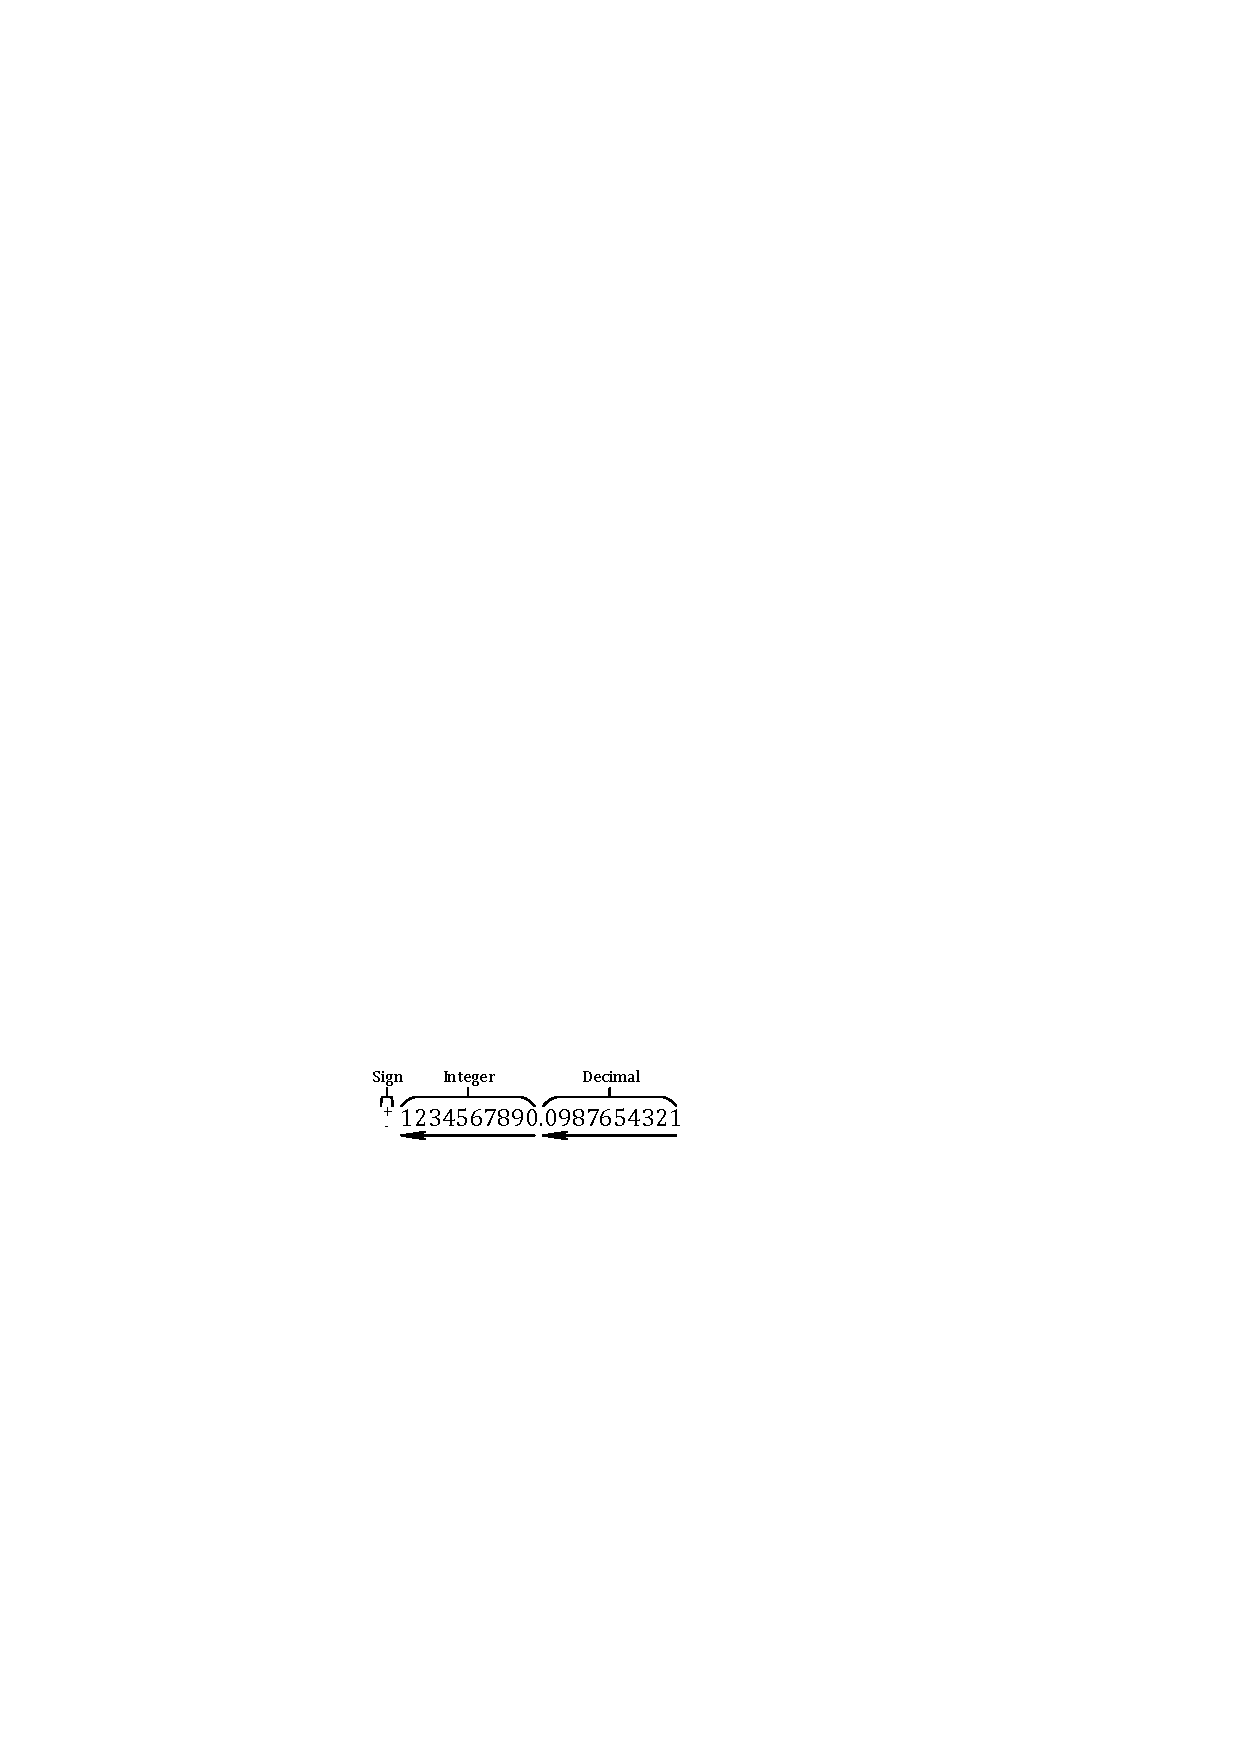
\includegraphics[scale=1.0]{./algorithm/real/pic/design/data_format_v3.pdf}
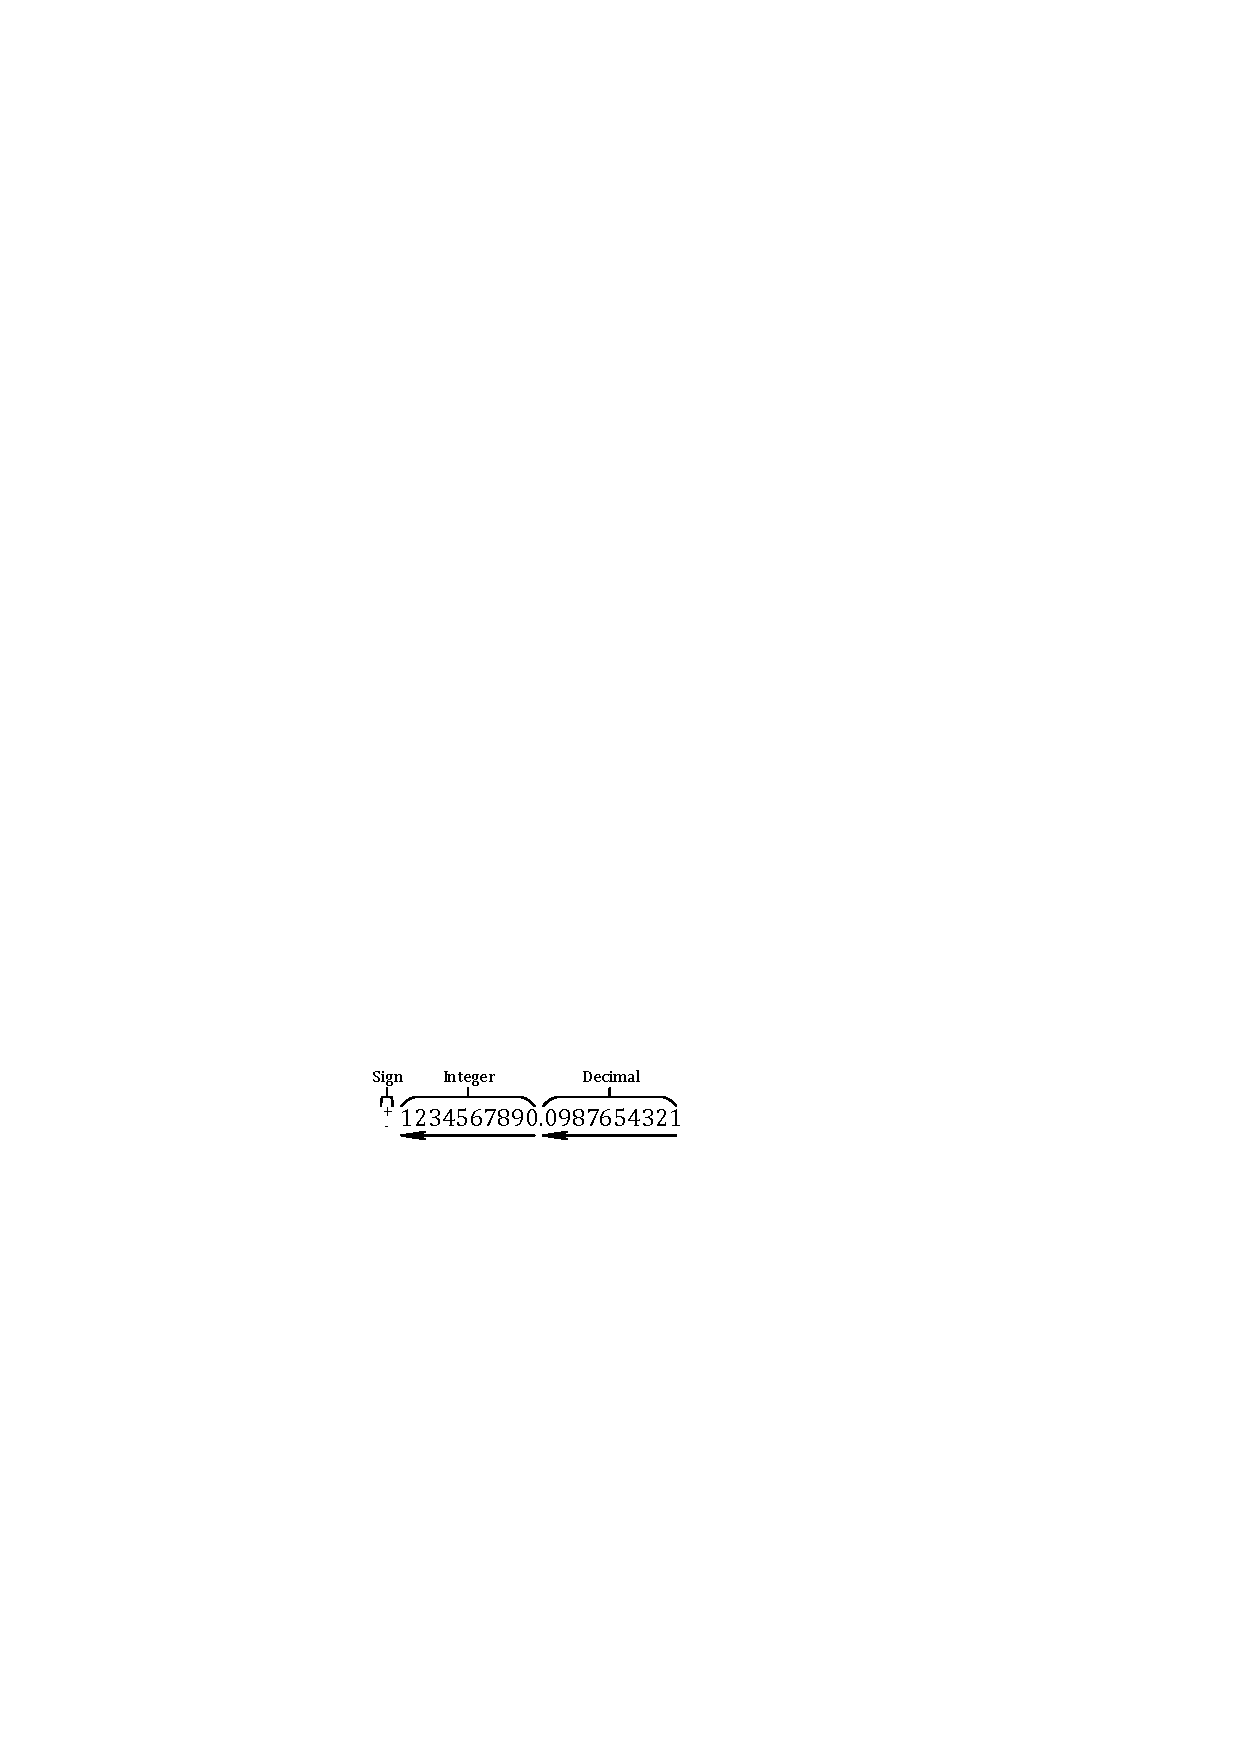
\includegraphics[width=0.6\textwidth]{./algorithm/real/pic/design/data_format_v3.pdf}
\caption{Data format of \textit{REAL} type.}
\label{fig:algorithm:real:data_format}
\end{figure}

The data format (figure \ref{fig:algorithm:real:data_format}) of \textit{REAL} is little bit different than the normal data concept, the value is as same as normal, the number at the left hand side means larger.\\

But when in the storage view is different, the \textit{"Integer"} part is store in normal and inverted order which will explain in the example of each operation, but the \textit{"Decimal"} part is using inverted which means the value will inverted when it stored. We use figure \ref{fig:algorithm:real:data_store_inverted} to explain why we do this.

\begin{figure}[h]
\centering
    \begin{subfigure}[b]{0.4\textwidth}
        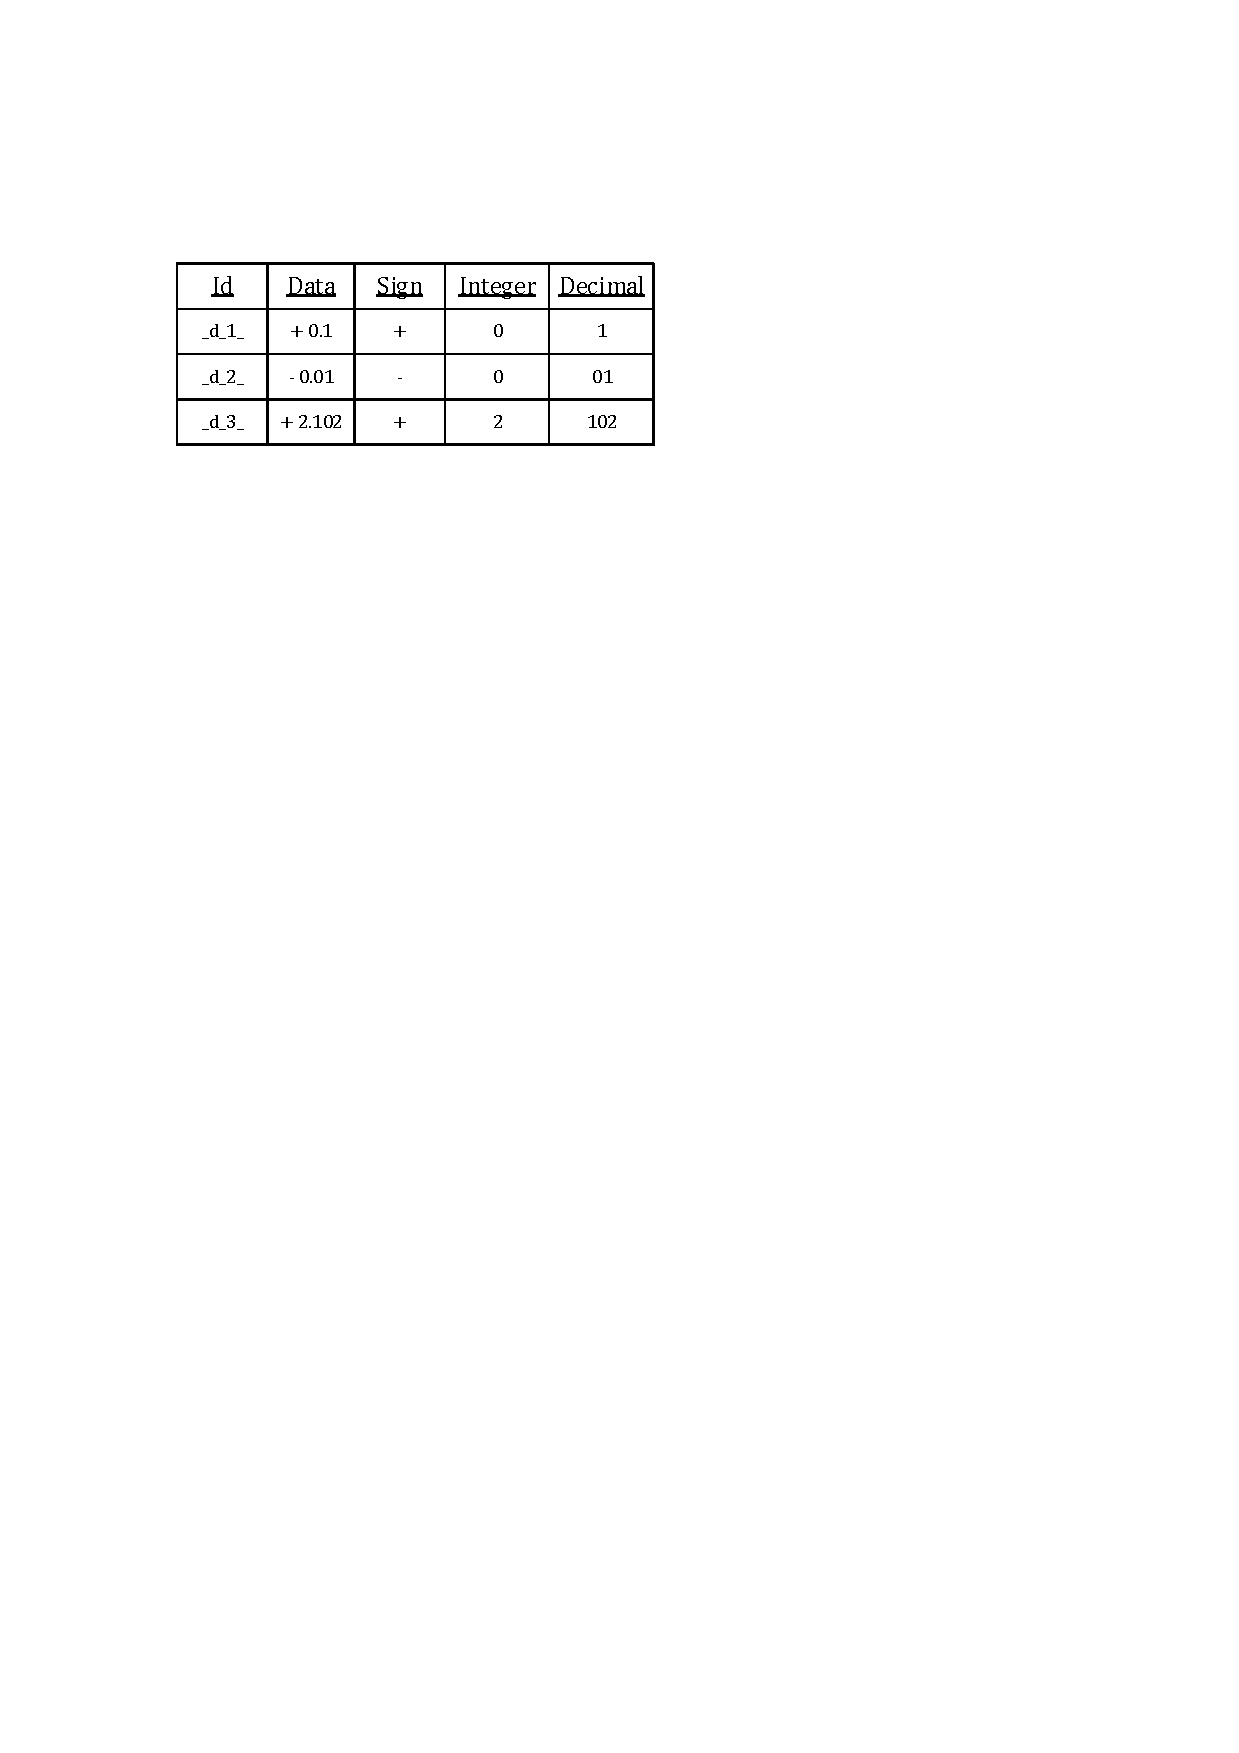
\includegraphics[width=\textwidth]{./algorithm/real/pic/design/data_store_inverted_1_v1.pdf}
        \caption{Normal order}
        \label{fig:algorithm:real:data_store_inverted_1}
    \end{subfigure}%
    ~ %add desired spacing between images, e. g. ~, \quad, \qquad etc.
          %(or a blank line to force the subfigure onto a new line)
    \begin{subfigure}[b]{0.4\textwidth}
        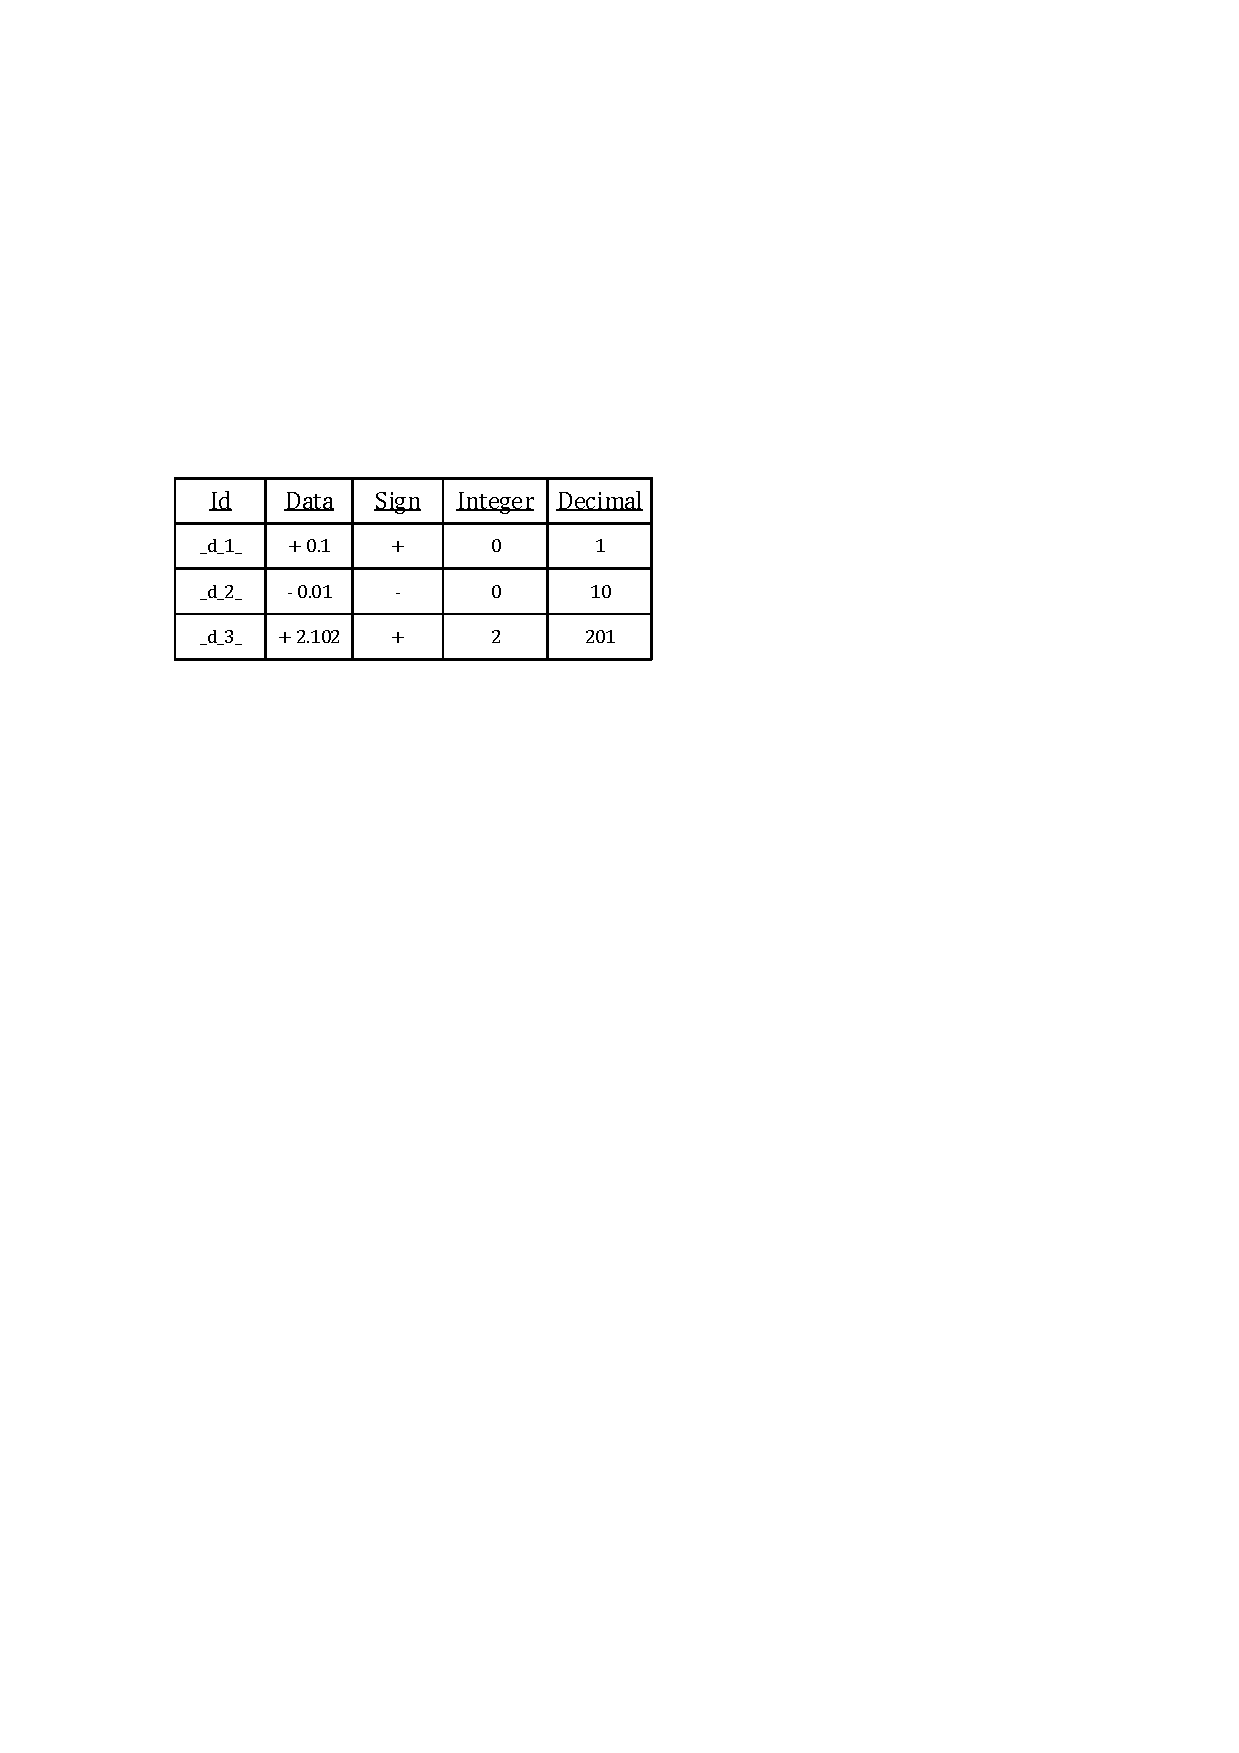
\includegraphics[width=\textwidth]{./algorithm/real/pic/design/data_store_inverted_2_v1.pdf}
        \caption{Inverted order}
        \label{fig:algorithm:real:data_store_inverted_2}
    \end{subfigure}

    \caption{Value storage}
    \label{fig:algorithm:real:data_store_inverted}
\end{figure}

If the data store as the same order as usual, the sample data will store like figure \ref{fig:algorithm:real:data_store_inverted_1}, the problem is if we treat \textit{'01'} as a value, it will convert into \textit{'1'} and lost its owns meaning, because \textit{'.1'} is not equal \textit{'.01'}. So if invert the \textit{"Decimal"} part, the value will look like figure \ref{fig:algorithm:real:data_store_inverted_2}. It shows the value can be store without missing value, the only is a additional convert operation is need to revert back into the real value when return data.\\

\begin{figure}[h]
\centering
%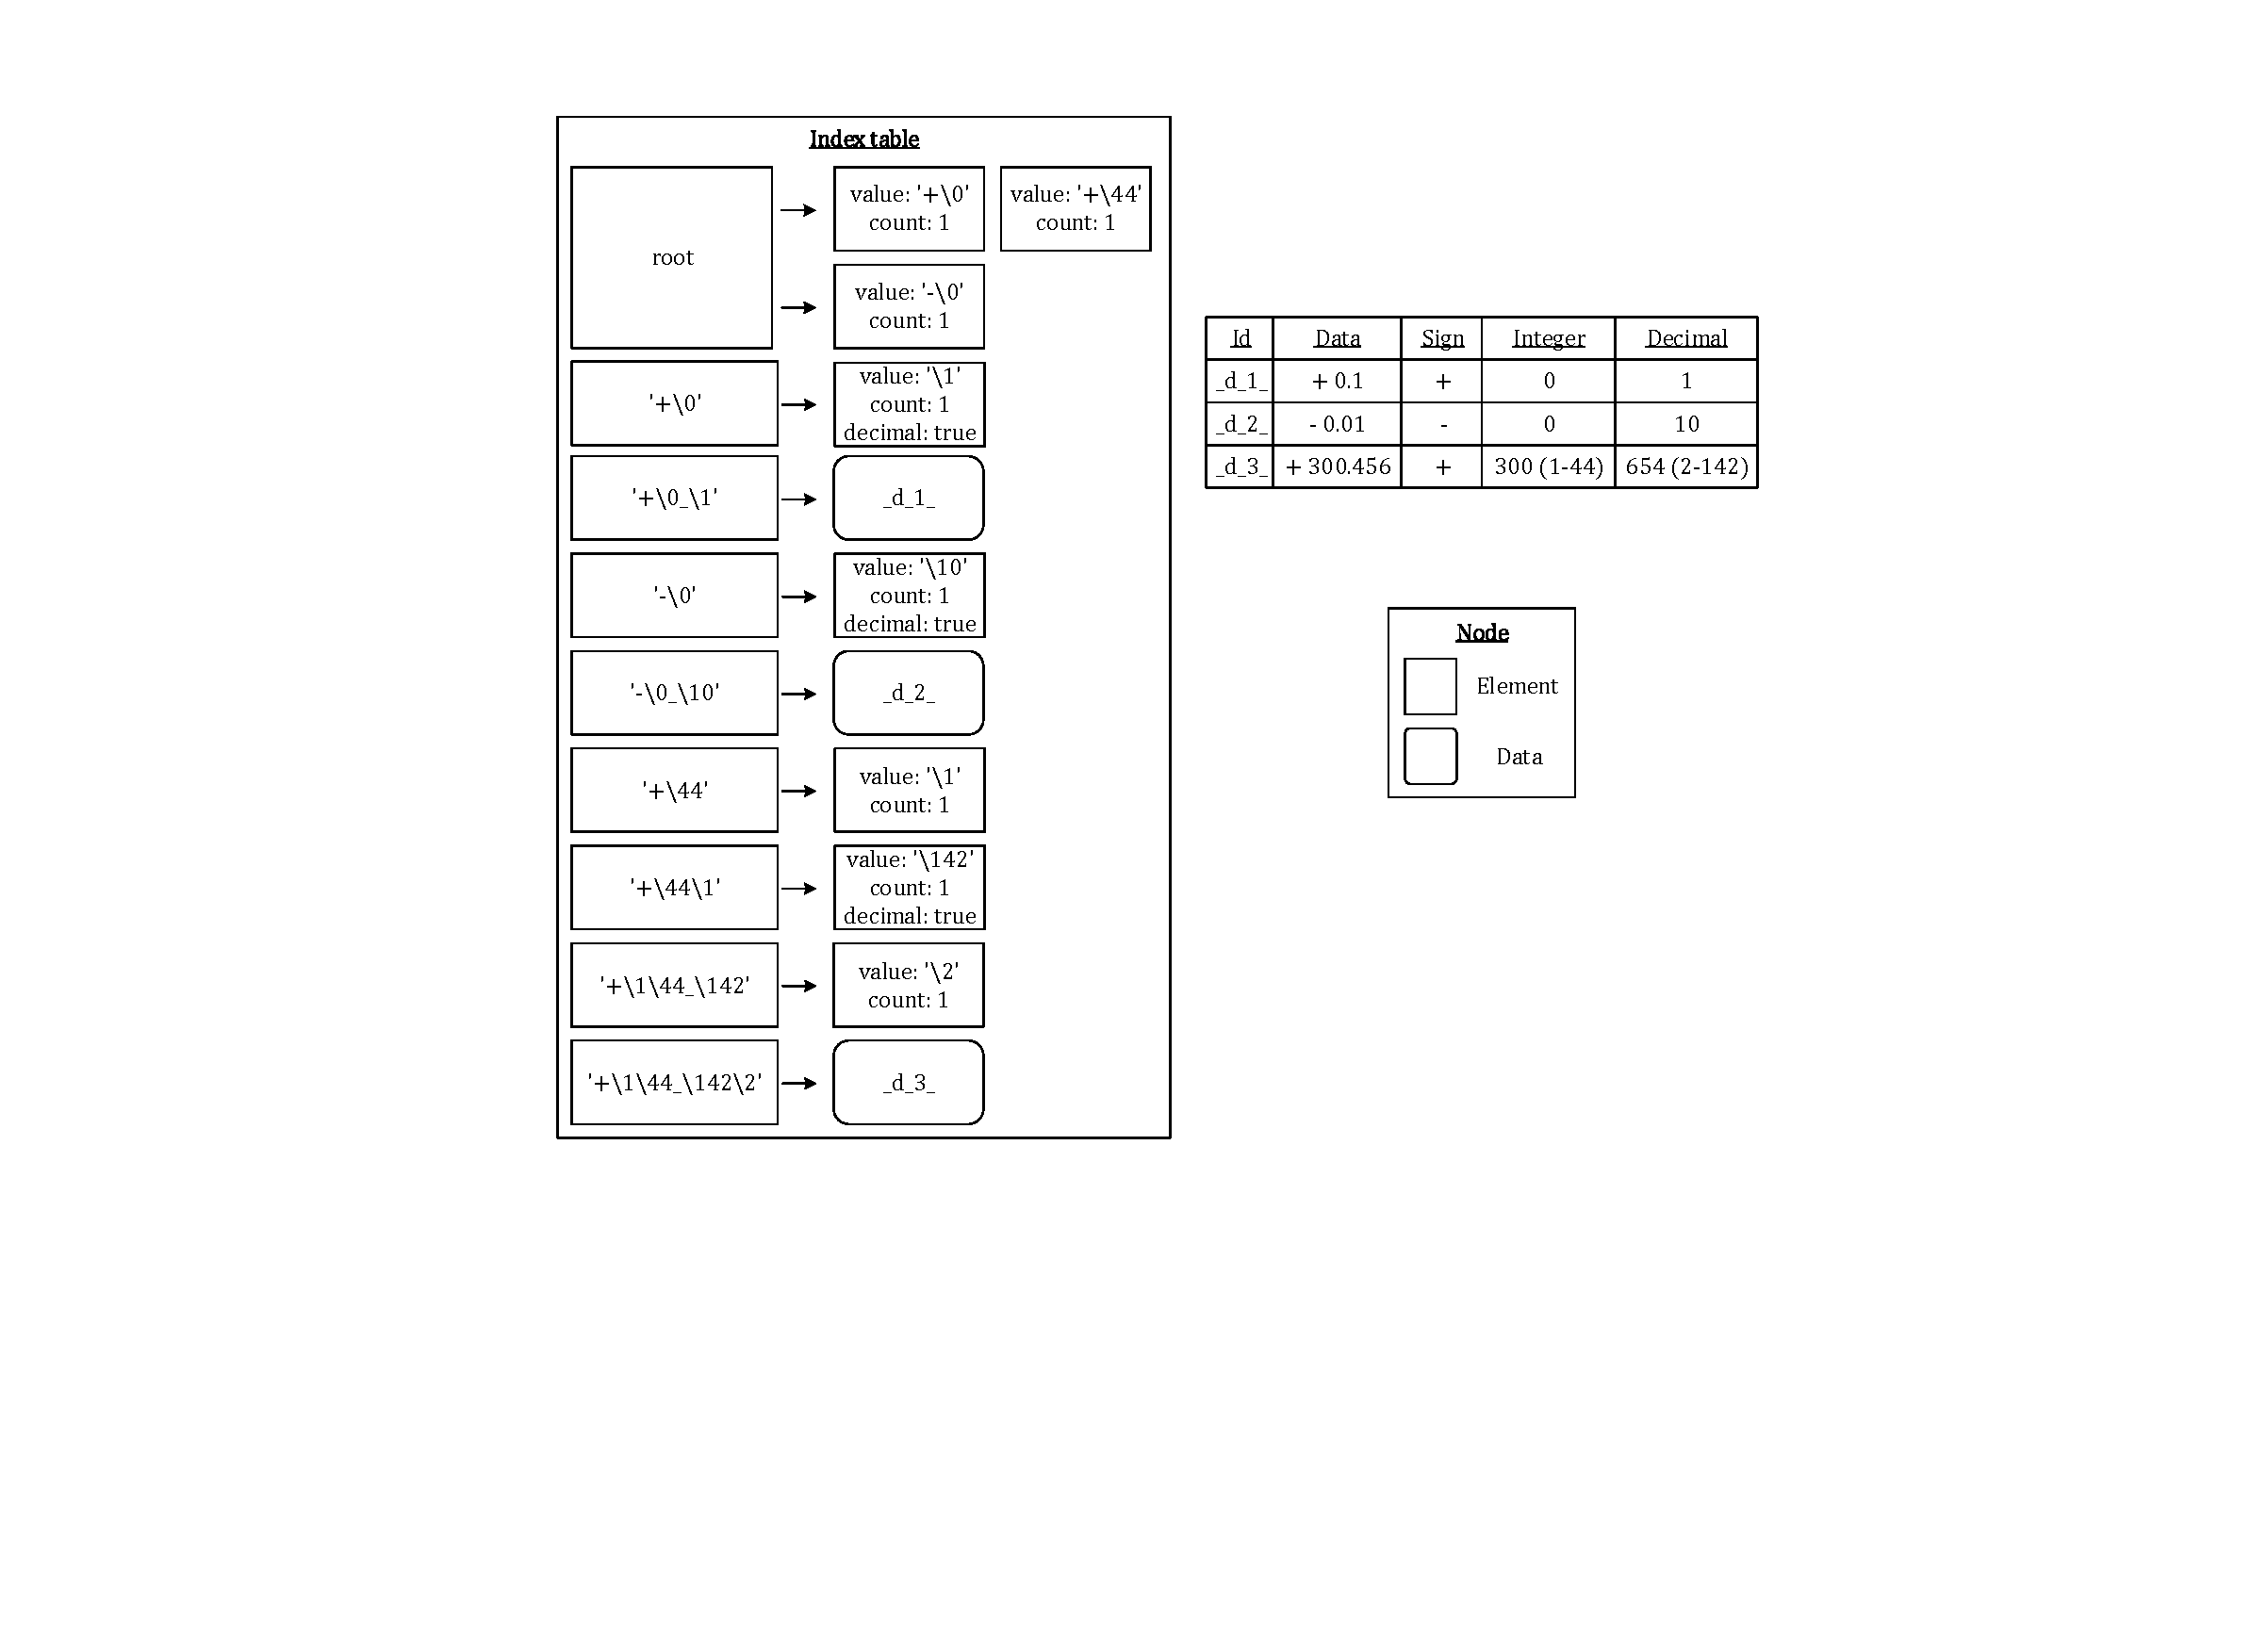
\includegraphics[scale=1.0]{./algorithm/real/pic/design/example_v4.pdf}
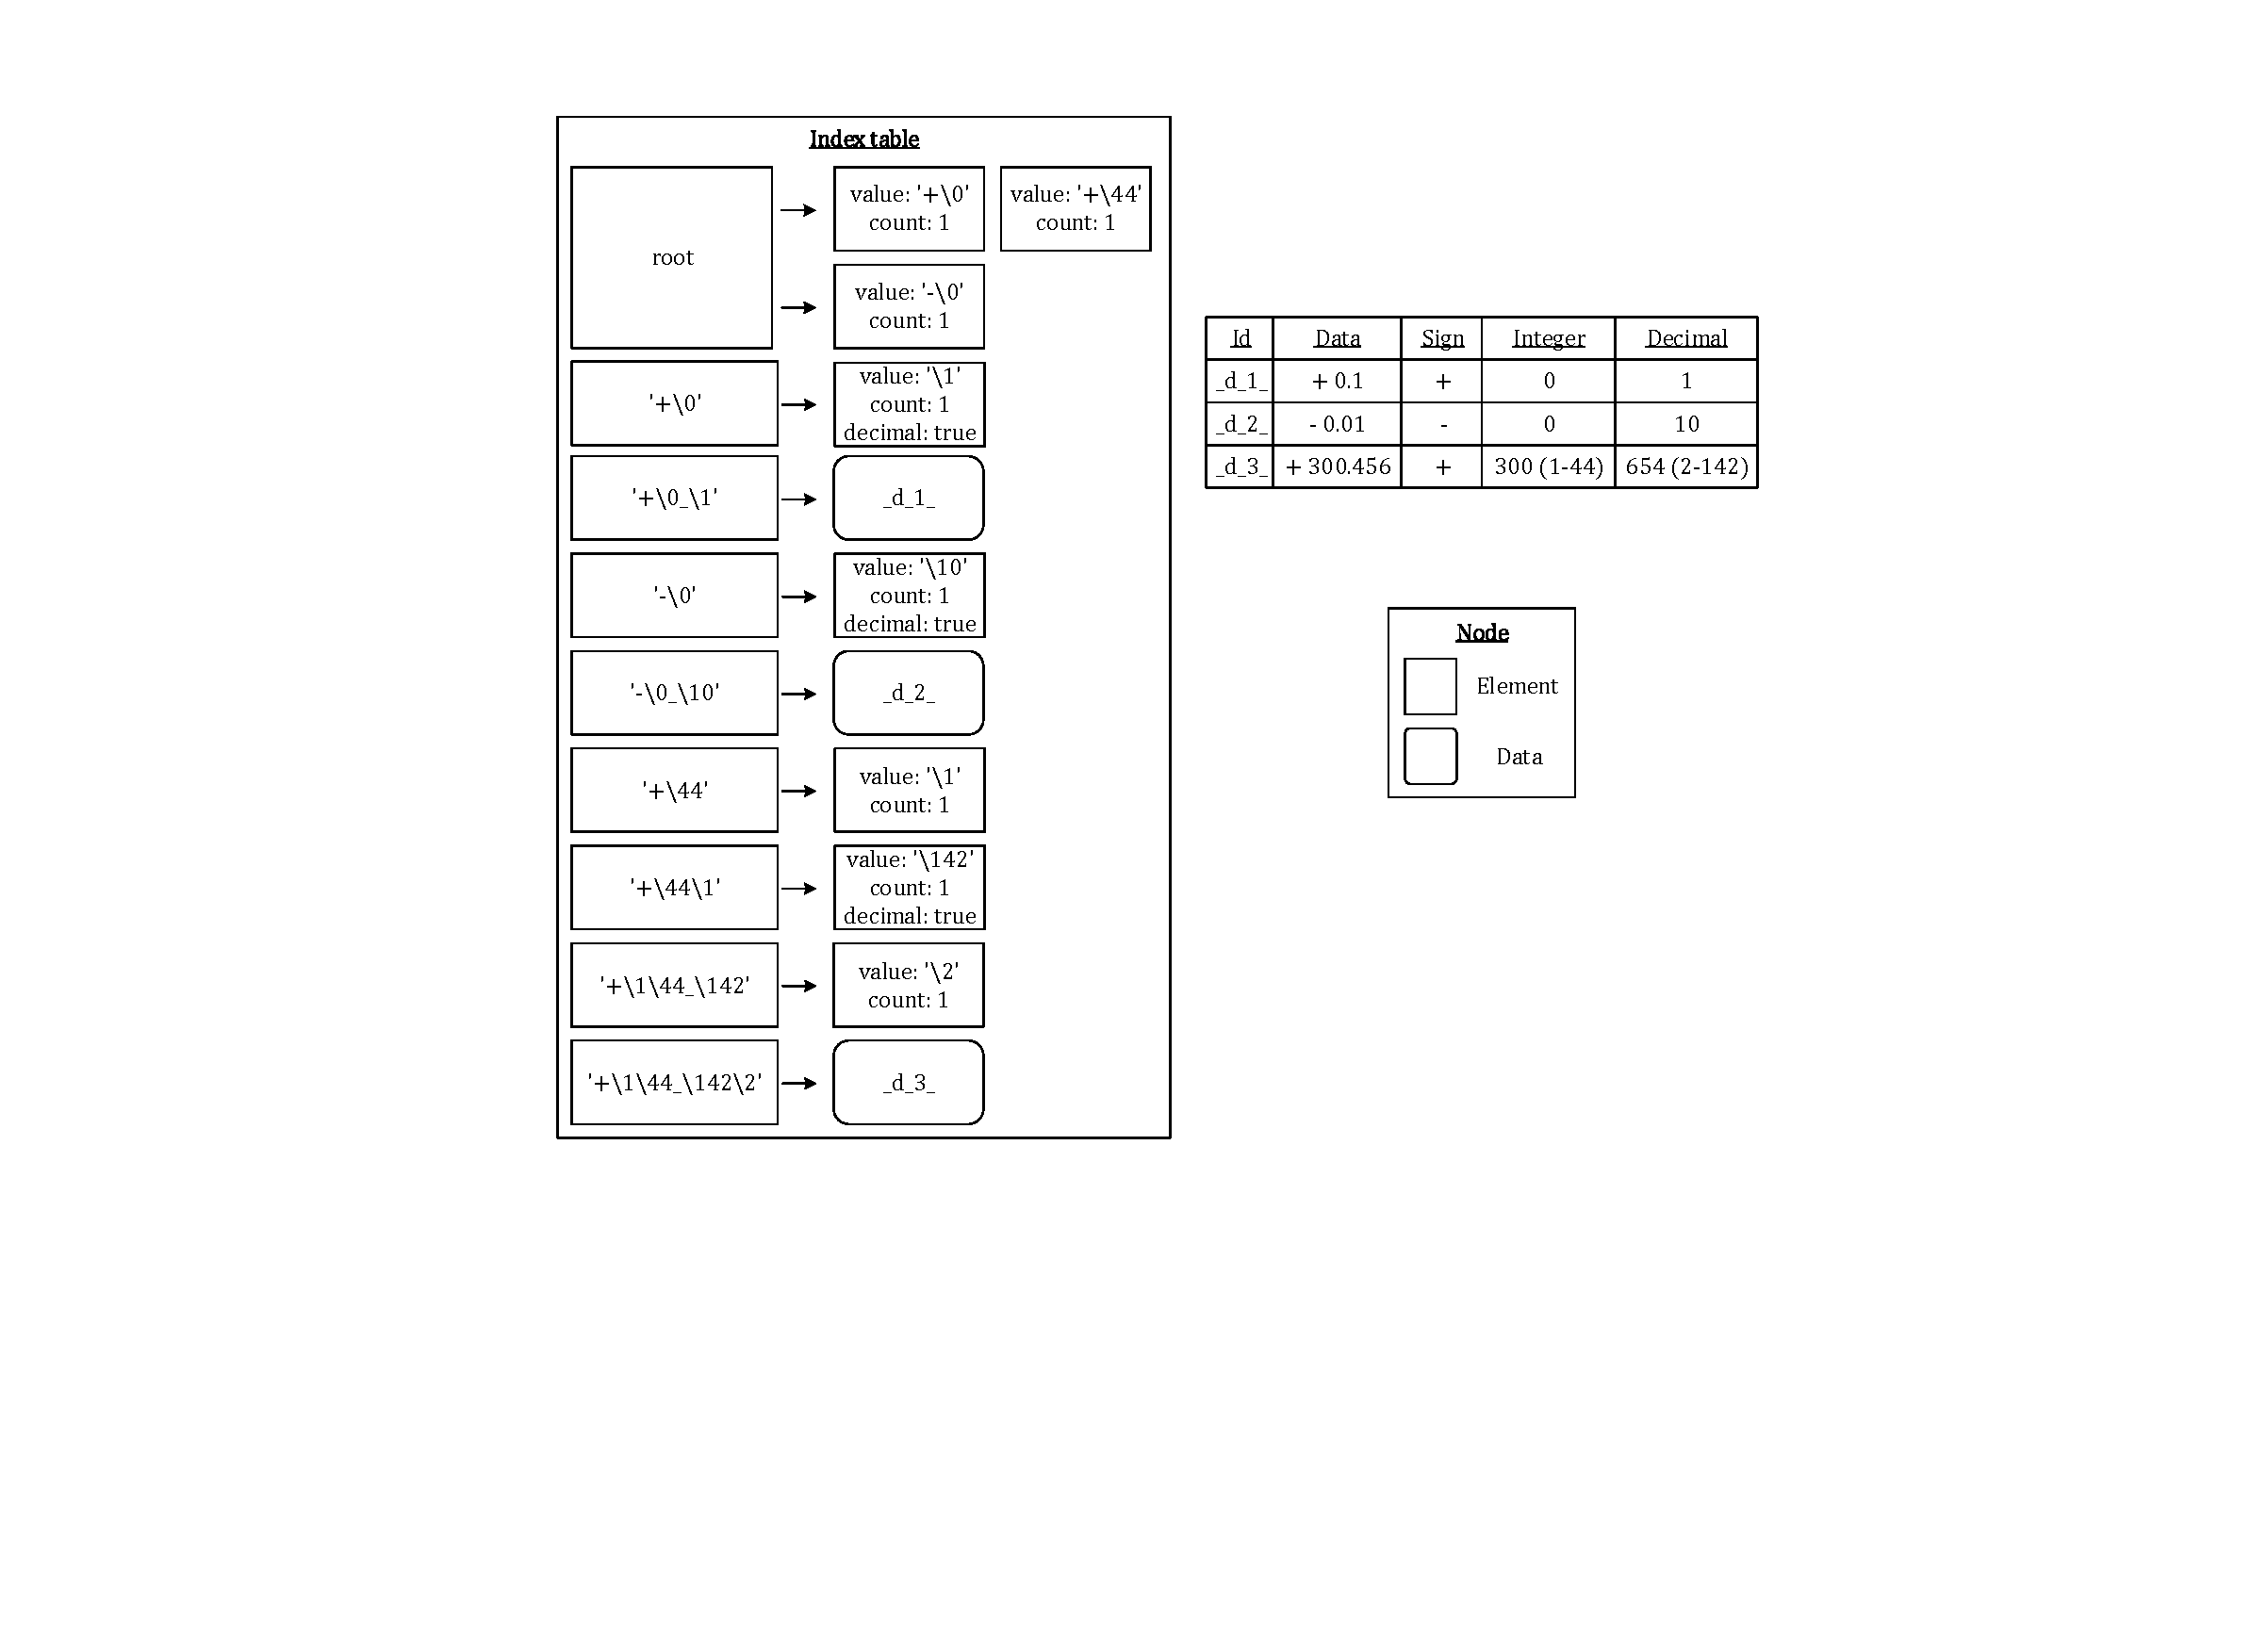
\includegraphics[width=0.8\textwidth]{./algorithm/real/pic/design/example_v4.pdf}
\caption{The index tables of \textit{REAL} type.}
\label{fig:algorithm:real:example}
\end{figure}

Figure \ref{fig:algorithm:real:example} is the example when storing data into index table. This table start with $root$ which is pointing to the \textit{"Sign"} part which is store with the last byte of \textit{"Integer"} part.

The \textit{"Integer"} is indexing using n-gram as normal, but it will index in two way:

\begin{enumerate}

\item When indexing the \textit{"Integer"} part only (like $'$+$\backslash44\backslash1'$ in figure), it is start from the last byte to the first, and then will pointing to the element node which contain a flag that means as $decimal$, which is represent to begin \textit{"Decimal"} part.

\item Like $'$+$\backslash1\backslash44\_\backslash2\backslash142'$ in figure, the order of the \textit{"Integer"} part is store as from the left to right when it is storing with the \textit{"Decimal"} part.

\end{enumerate}

And \textit{"Decimal"} is store from right to left, and because the inverted string value design which means if the value is small then it will become a greater value.

This order of \textit{"Integer"} and \textit{"Decimal"} part design is because this can do faster searching the key when doing sorting and comparison, this will explan detail in fellowing section.

% Insertion section
\subsubsection{Insertion}

In description and figure \ref{fig:algorithm:real:example} have already mentioned some of the flow of insertion, so in here will show the table if insert another value into the table. Insert $\pi (3.14159)$ into table, which will become like figure \ref{fig:algorithm:real:insertion:example}.

\begin{figure}[h]
\centering
%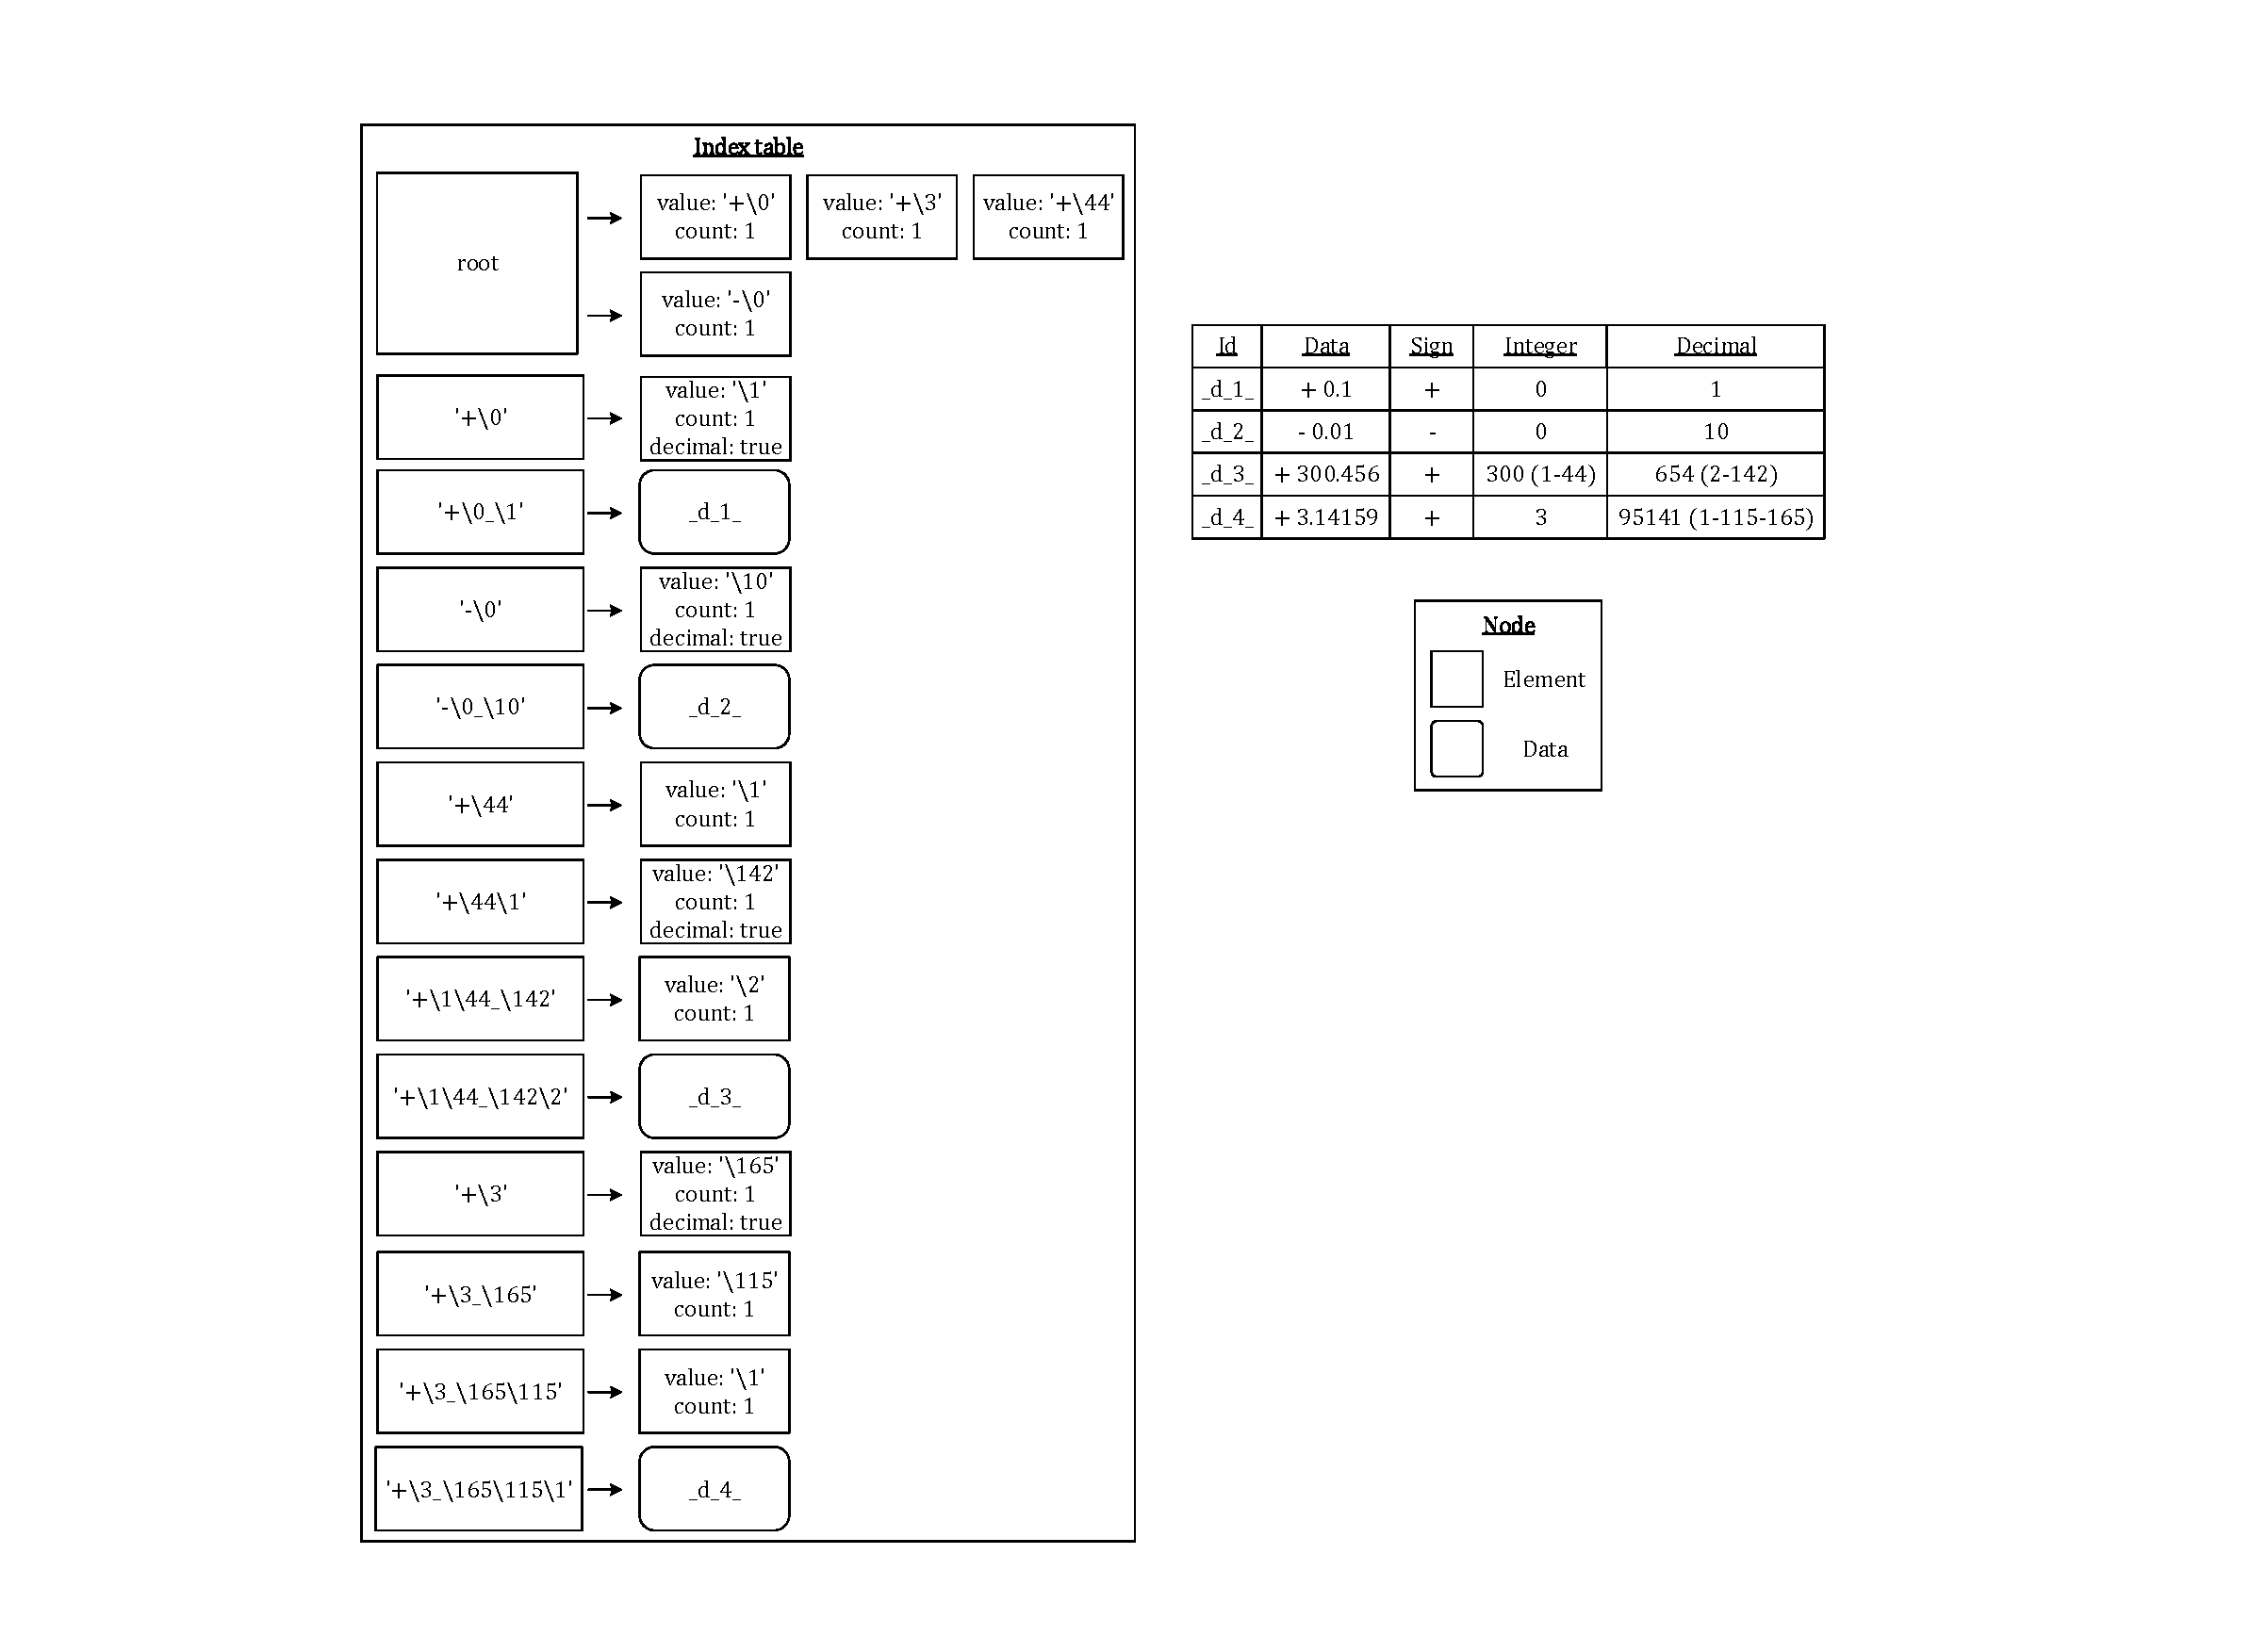
\includegraphics[scale=0.45]{./algorithm/real/pic/insertion/example_v4.png}
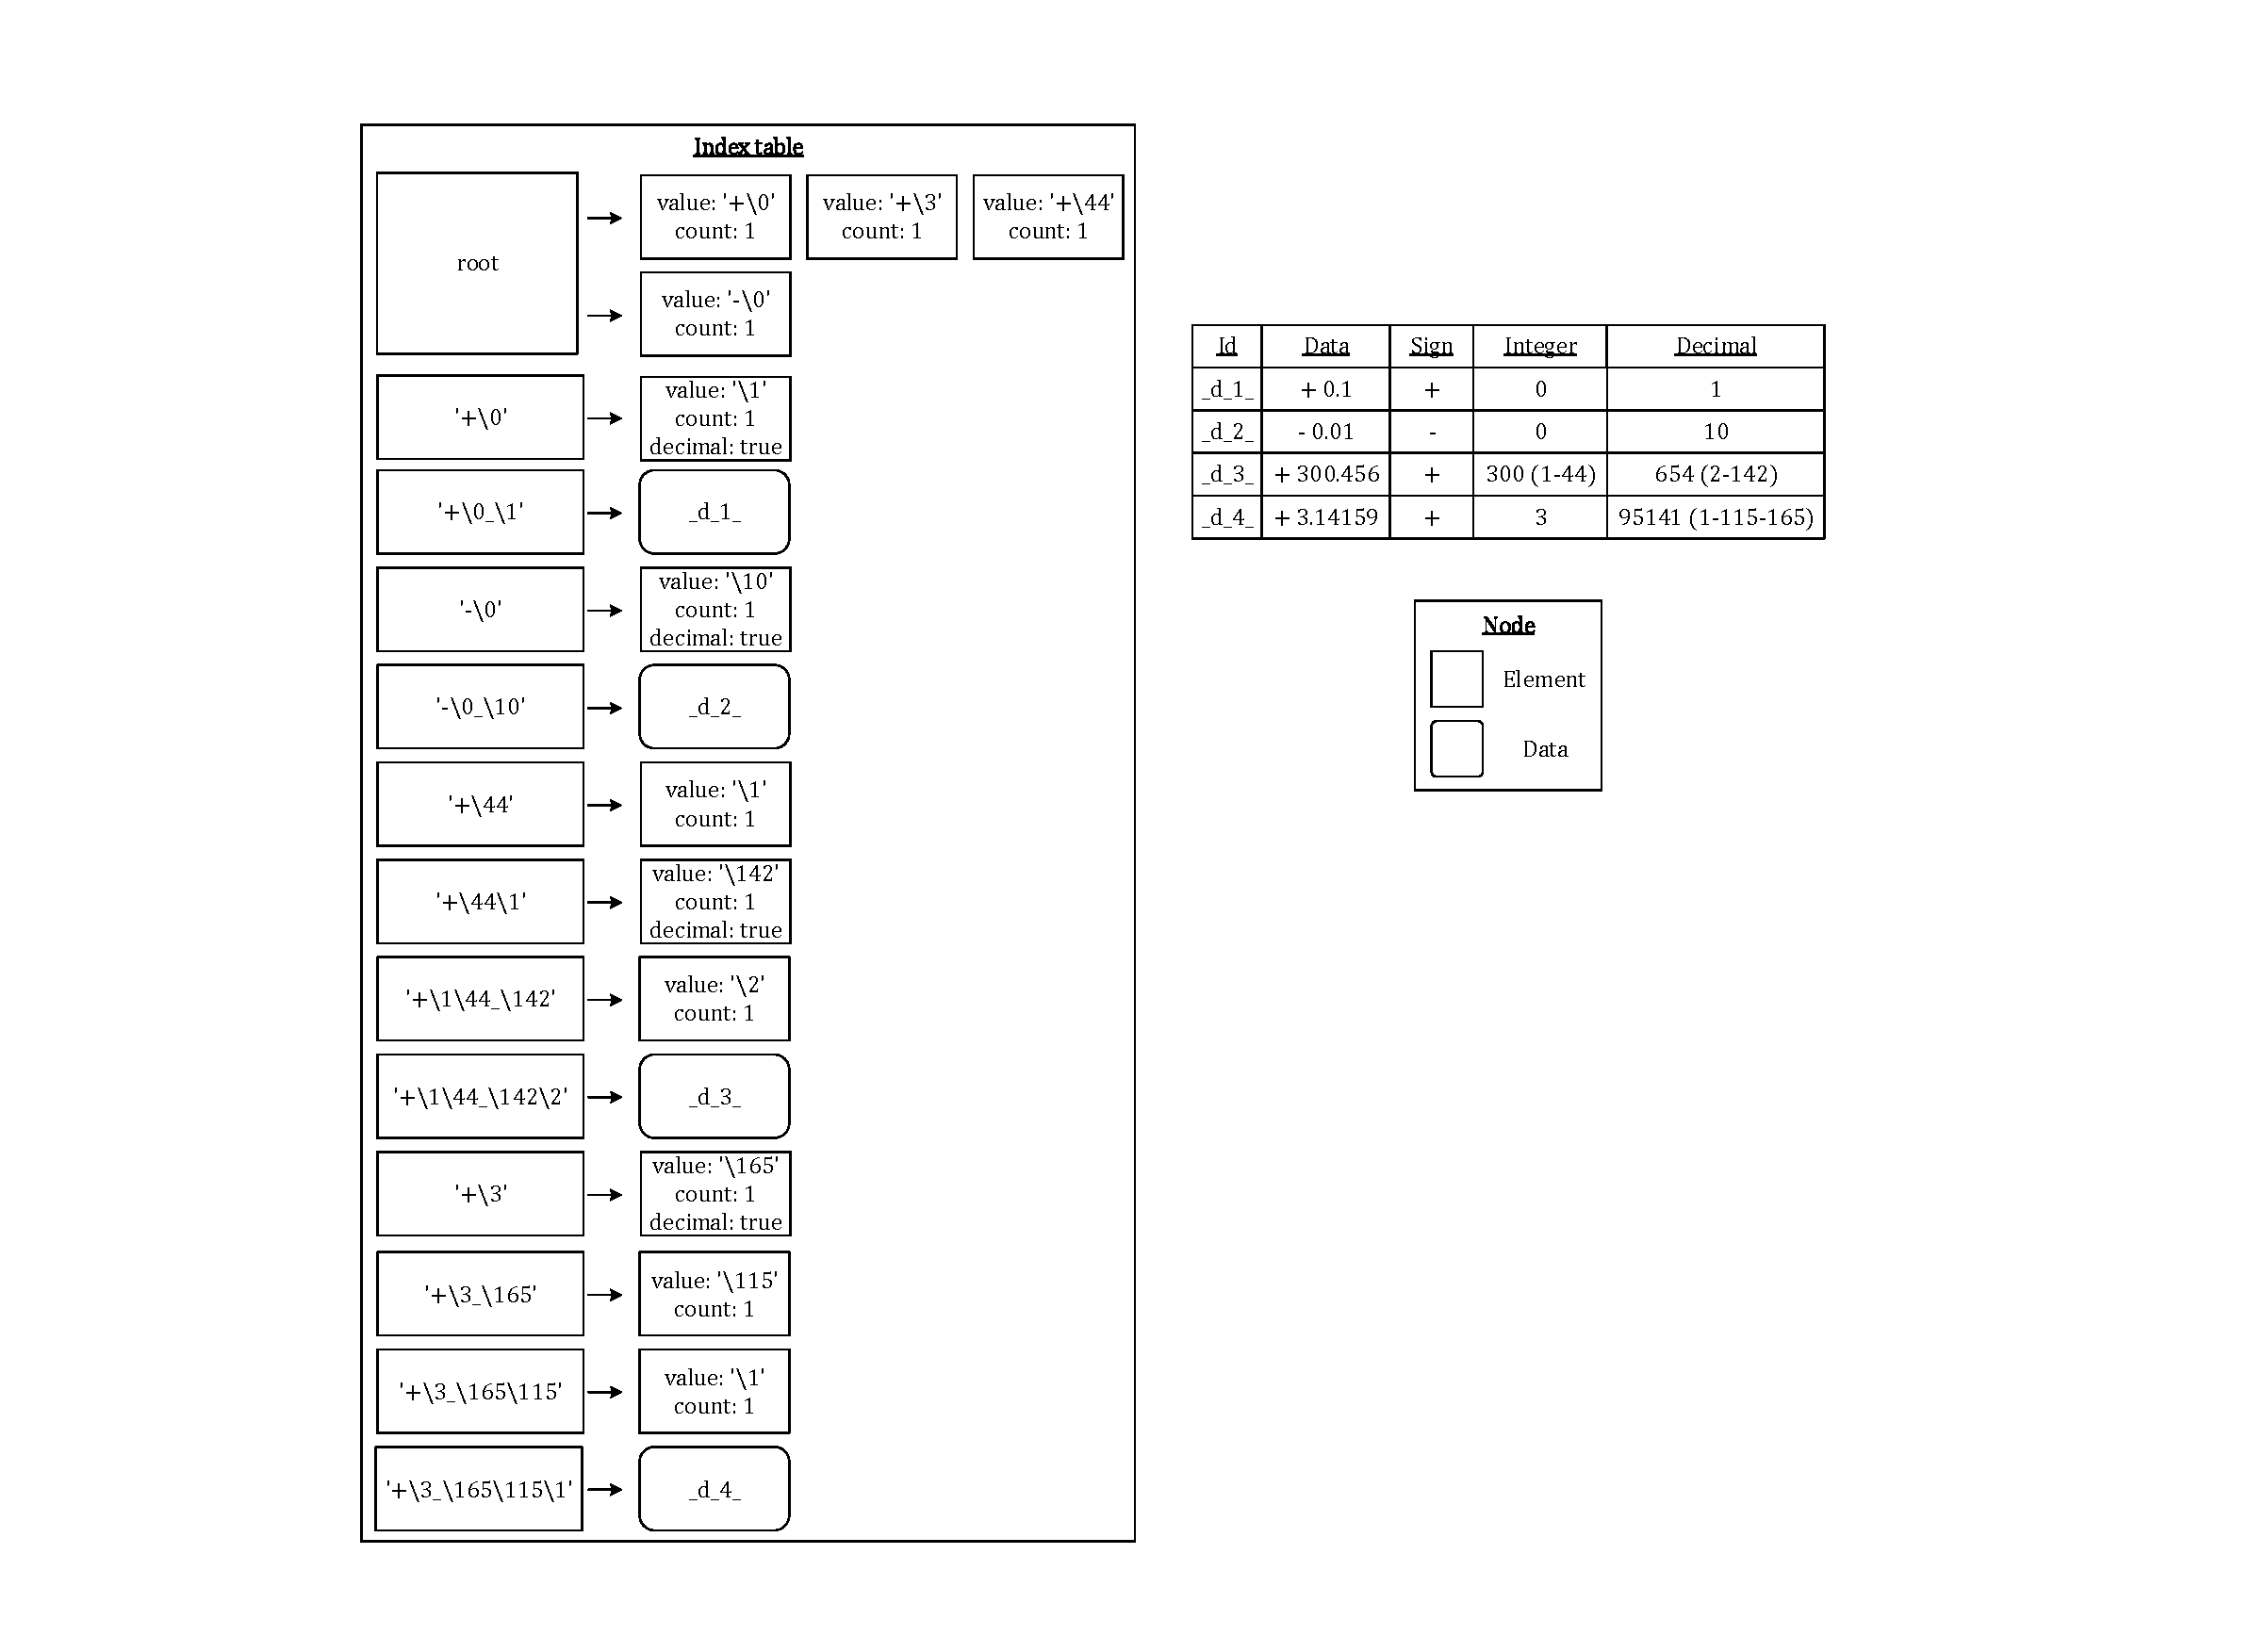
\includegraphics[width=0.8\textwidth]{./algorithm/real/pic/insertion/example_v4.pdf}
\caption{The table after inserted $\pi (3.14159)$.}
\label{fig:algorithm:real:insertion:example}
\end{figure}

Figure \ref{fig:algorithm:real:insertion:example} shows that the $\pi (+3.14159)$ is store the value by its \textit{"Sign"} $(+)$, \textit{"Integer"} $(3)$ and \textit{"Decimal"} $(95141)$.

The \textit{"Sign"} is pointing the last byte of the \textit{"Integer"}, the reason of point to the last byte is because of the dynamic length of \textit{REAL}, also assume the the byte of the data is longer than the input byte length:

\begin{enumerate}

\item  If the \textit{"Sign"} is pointing the first byte, then when we search the result for the input, this may need to compare more byte or we need to get the whole \textit{"Integer"} in the worst case to sure that this value is suitable or not to the input.

\item If \textit{"Sign"} is pointing the last byte, then we just need to compare few bytes or the same byte length of the input that we can immediately to know that is a result or not. So this indexing can speed up the searching.

\end{enumerate}

Time complexity should be $O(b!)$ which domain as $O(b)$, and $b$ is the length of the byte needed where $b = 4$ in this case.



% Deletion section
\subsubsection{Deletion}

Deletion is just do the opposite insertion to remove the byte and decrease the count. So time complexity be $O(b)$.



% Modification section
\subsubsection{Modification}

The modify flow are similar as \textit{INTEGER} type, remove the key which don't needed and add the count if the byte is the same. So follow the example in figure \ref{fig:algorithm:real:insertion:example} and then modify -$0.01$ to +$0.0$ (because zero don't contain positive or negative sign, so using positive sign should be fine), the table will look like figure \ref{fig:algorithm:real:modification:example} and the time complexity be $O(b)$.

\begin{figure}[h]
\centering
%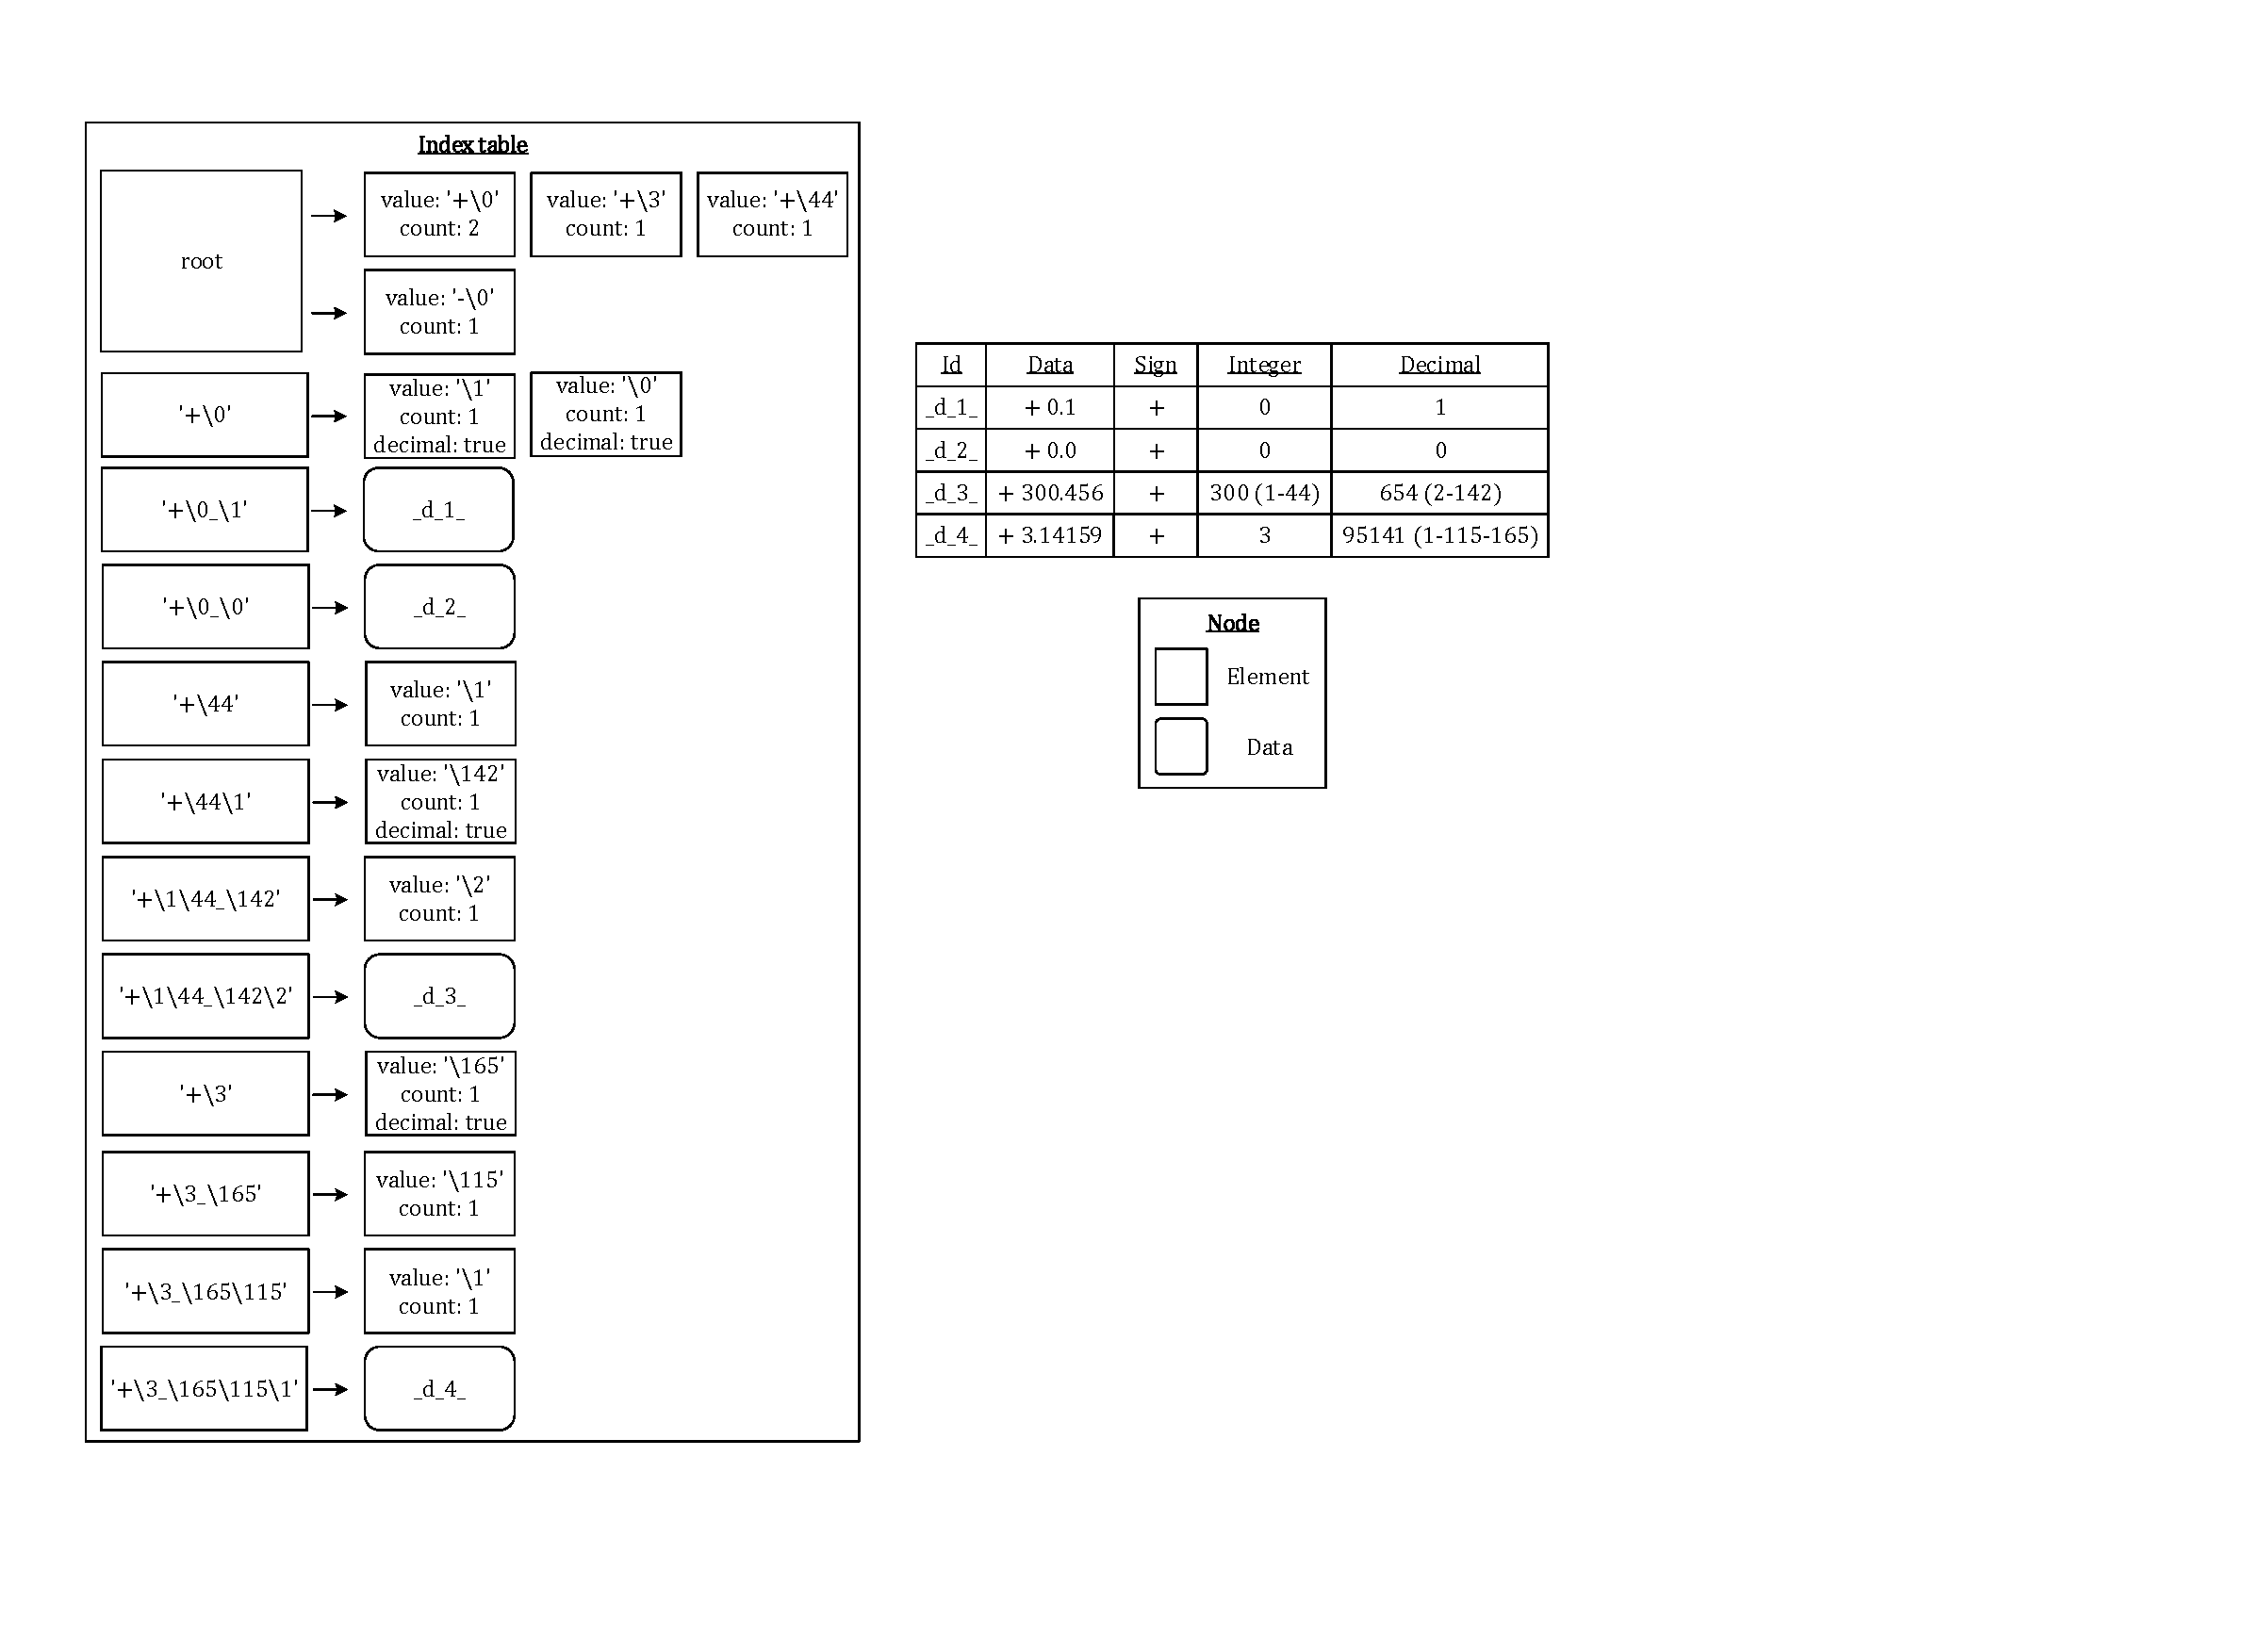
\includegraphics[scale=0.5]{./algorithm/real/pic/modification/example_v4.pdf}
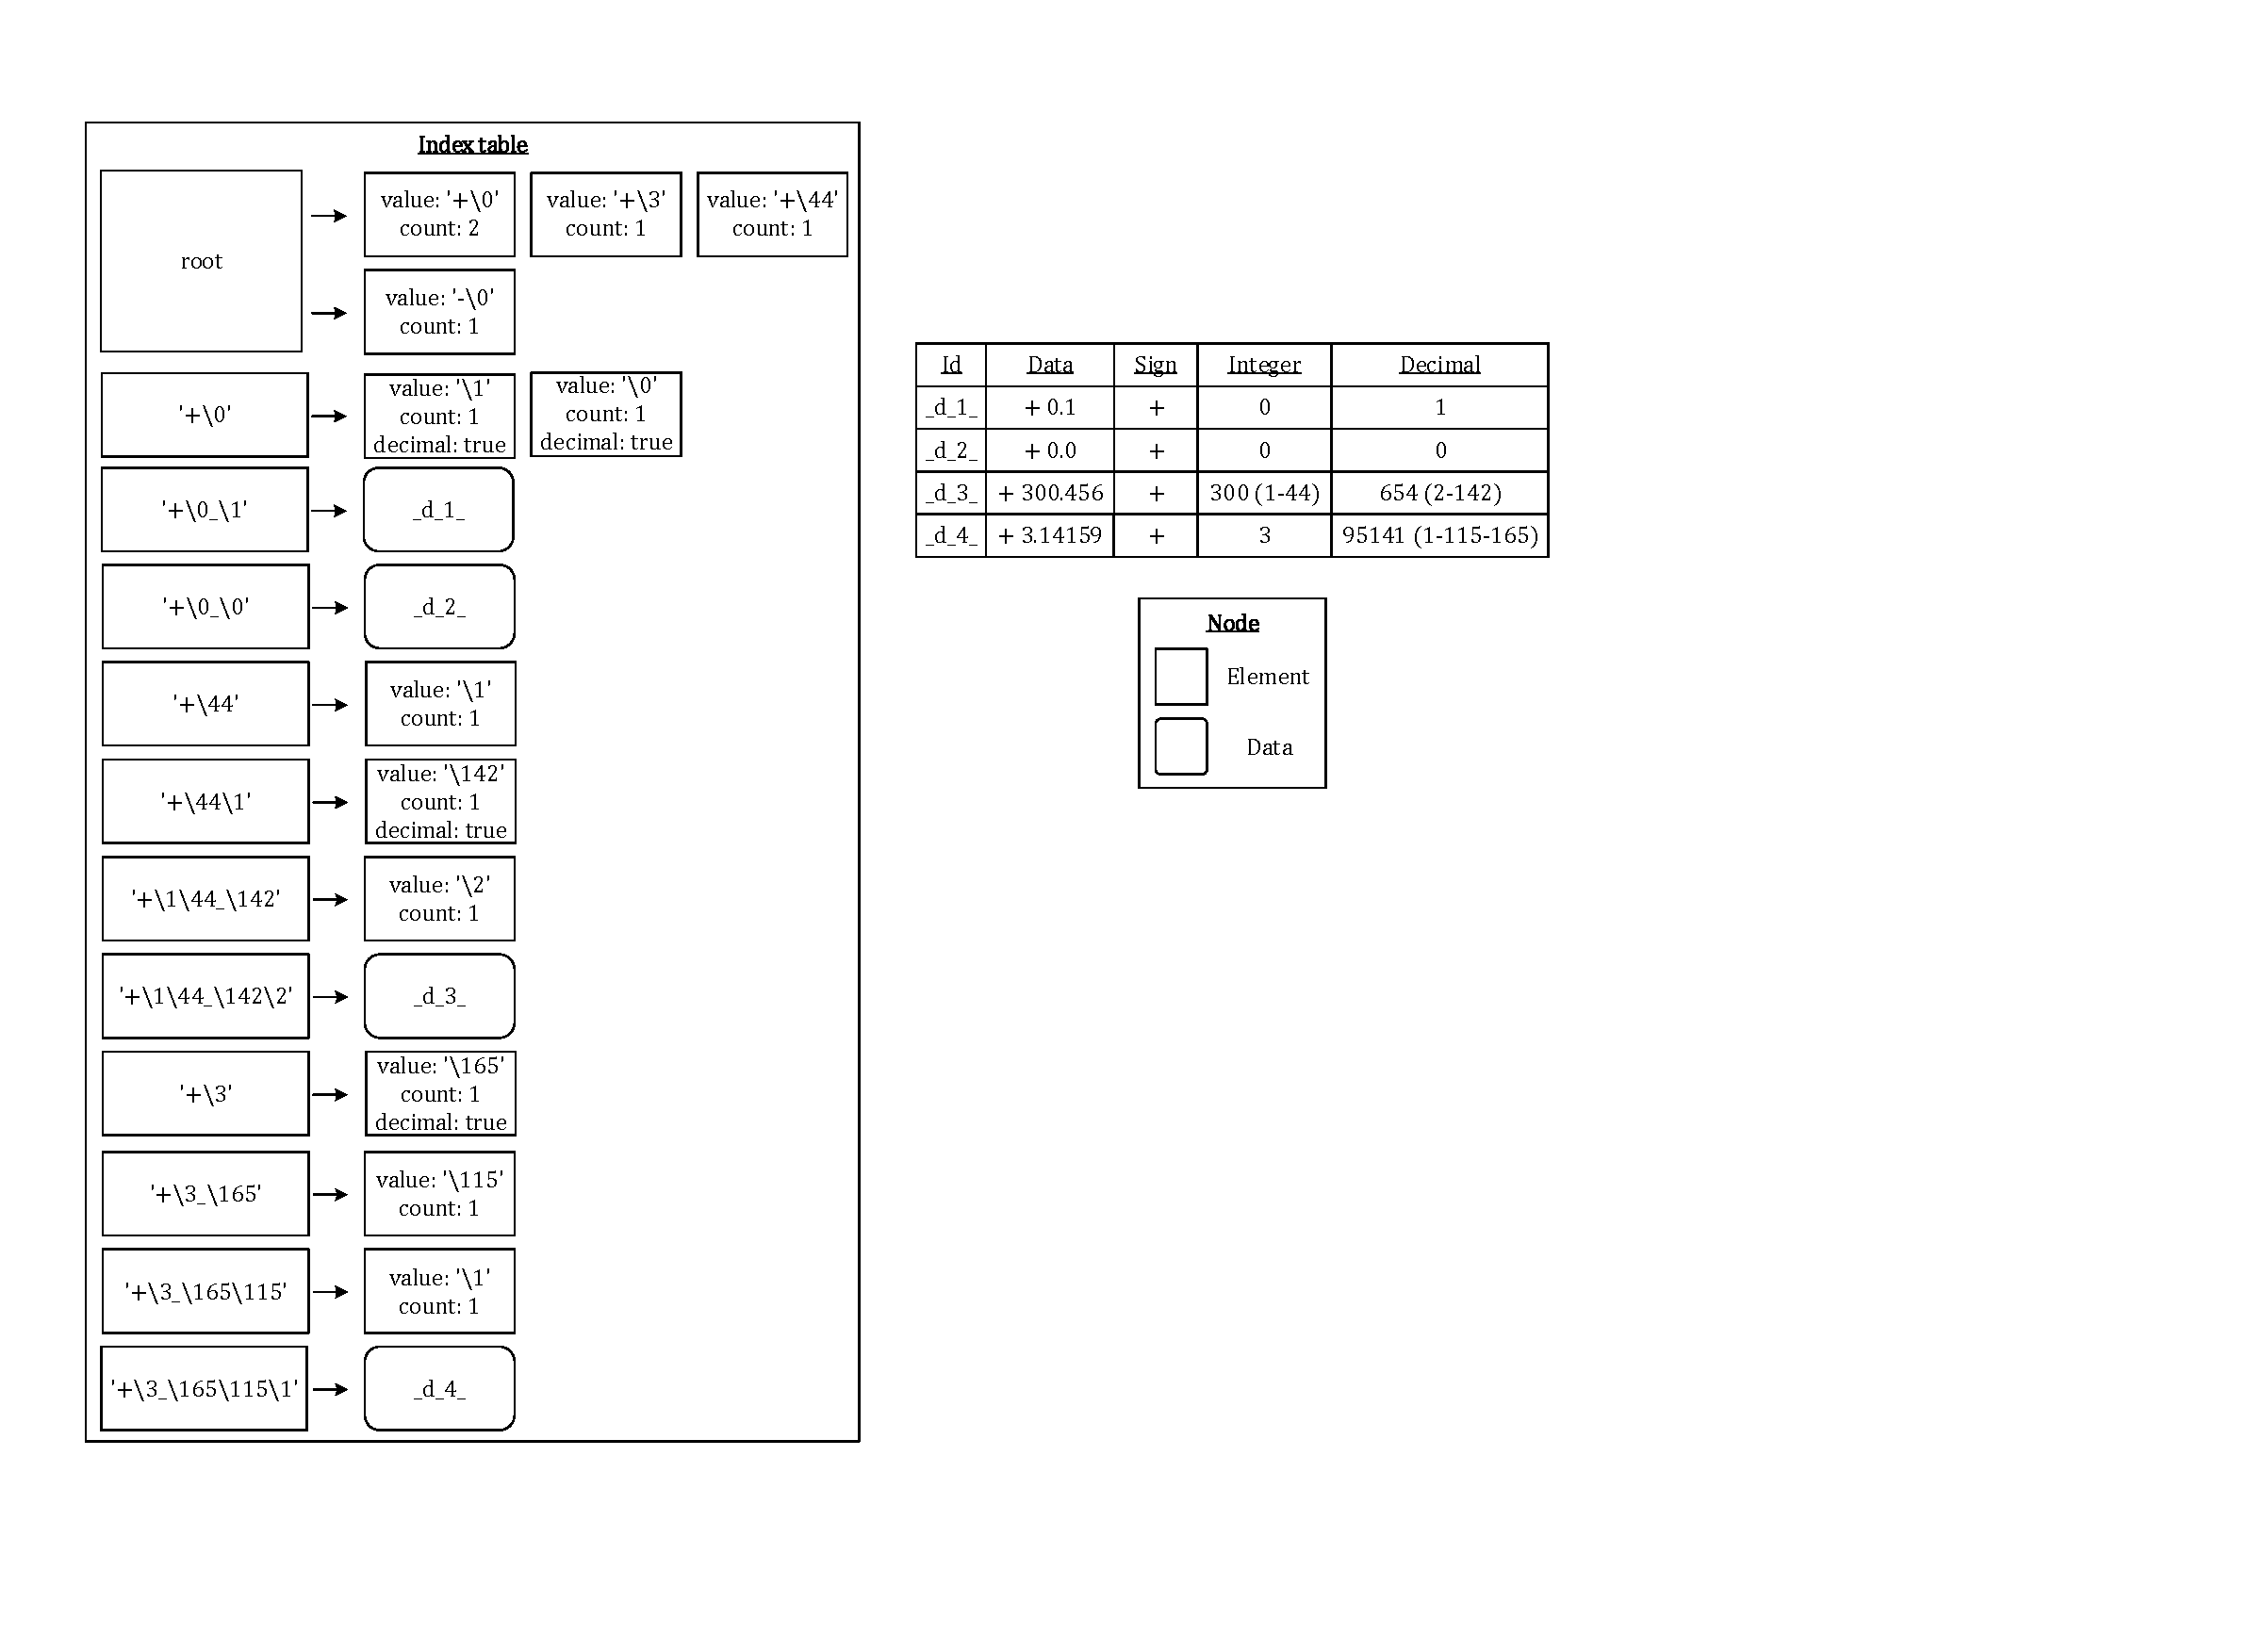
\includegraphics[width=0.8\textwidth]{./algorithm/real/pic/modification/example_v4.pdf}
\caption{The table after modified the value.}
\label{fig:algorithm:real:modification:example}
\end{figure}



% Selection section
\subsubsection{Selection}

The follow operations will use figure \ref{fig:algorithm:real:modification:example} as the example.

% Selection section enumerate
\begin{enumerate}

% --------------------------------------------------------

% Equal
\item \textbf{Equal}

If search \textit{0.0}, then convert it into three part: \textit{"Sign"}, \textit{"Integer"} and \textit{"Decimal"}, which means $'$+$\backslash0\backslash\_\backslash0'$ and use this as key to get the result, this should take $O(1)$.

% --------------------------------------------------------

% Not equal
\item \textbf{Not equal}

If searching the result which is not equal \textit{0.0}, strat of convert it into key, then start from root, then recursively to find the data nodes and only skip the key of input. This operation should take $O(b)$.

% --------------------------------------------------------

% Less than
\item \textbf{Less than}

When comparing the \emph{"Less than"} or \emph{"Greater}, the flow is way different as the other because of the dynamic byte design.

For example searching \textit{300.0} in table, then convert into string $'$+$\backslash44\backslash1\_\backslash0'$ which the length of \textit{"Integer"} is \textit{2} and \textit{1} for \textit{"Decimal"} that the two value is use to let the compare function know how deep of the byte need to search.

% Less than section enumerate
\begin{enumerate}

% Input value is a negative value
\item \textbf{Input value is a negative value}

\begin{enumerate}

\item Start from root and only get the nodes which the \textit{"Sign"} are \textit{'-'}.

\item When searching \textit{"Integer"} part, recursively to search the element node contain \textit{decimal} with the length is \textit{"longer than or equal to"} to the \textit{"Integer"} length of input (in this case is \textit{2}). Then only remain the nodes that the value of \textit{"Integer"} is \textit{"larger than or equal to"} the value in \textit{"Integer"} part of input.

\item Searching in \textit{"Decimal"} part:
\begin{enumerate}

\item If the length of \textit{"Integer"} part is \textit{"longer than"} the input, then get all the data nodes.

\item If the length of \textit{"Integer"} part is \textit{"equal to"} the input, then recursively and only get the element nodes that the length is \textit{"greater than or equal to"} the length of \textit{"Decimal"} of input. And check the value of \textit{"Decimal"} is \textit{"larger than"} the value in \textit{"Decimal"} part of input.
\end{enumerate}

\end{enumerate}

% Input value is a positive value
\item \textbf{Input value is a positive value}

\begin{enumerate}

\item Get all the data nodes start from root which the \textit{"Sign"} are \textit{'-'}.

\item Next start from root and get the nodes which the \textit{"Sign"} are \textit{'+'}.

\item When searching \textit{"Integer"} part, recursively to search the element node contain \textit{decimal} with the length is \textit{"shorter than or equal to"} to the \textit{"Integer"} length of input (in this case is \textit{2}). Then only remain the nodes that the value of \textit{"Integer"} is \textit{"smaller than or equal to"} than the value in \textit{"Integer"} part of input.

\item Searching in \textit{"Decimal"} part:
\begin{enumerate}

\item If the length of \textit{"Integer"} part is \textit{"shorter than"} the input, then get all the data nodes.

\item If the length of \textit{"Integer"} part is \textit{"equal to"} the input, then recursively and only get the element nodes that the length is \textit{"shorter than or equal to"} the length of \textit{"Decimal"} of input. And check the value of \textit{"Decimal"} is \textit{"smaller than"} the value in \textit{"Decimal"} part of input.
\end{enumerate}

\end{enumerate}

% Input value is equal to 0.0
\item \textbf{Input value is equal to \textit{0.0}}

Get all the data nodes start from root which the \textit{"Sign"} are \textit{'-'}.

% End Less than section enumerate
\end{enumerate}

The \emph{"Less than or equal to"} comparison is just do the \emph{"Less than"} and \emph{"Equal"} operation and then combine both result for ouput. The time complexity is $O(b)$ for both operation.

% --------------------------------------------------------

% Greater than
\item \textbf{Greater than}

This comparison flow is similar as \emph{"Less than"}.

% Greater than section enumerate
\begin{enumerate}

% Input value is a negative value
\item \textbf{Input value is a negative value}

\begin{enumerate}

\item Get all the data nodes start from root which the \textit{"Sign"} are \textit{'+'}.

\item Next start from root and get the nodes which the \textit{"Sign"} are \textit{'-'}.

\item When searching \textit{"Integer"} part, recursively to search the element node contain \textit{decimal} with the length is \textit{"shorter than or equal to"} to the \textit{"Integer"} length of input. Then only remain the nodes that the value of \textit{"Integer"} is \textit{"larger than or equal to"} than the value in \textit{"Integer"} part of input.

\item Searching in \textit{"Decimal"} part:
\begin{enumerate}

\item If the length of \textit{"Integer"} part is \textit{"shorter than"} the input, then get all the data nodes.

\item If the length of \textit{"Integer"} part is \textit{"equal to"} the input, then recursively and only get the element nodes that the length is \textit{"shorter than or equal to"} the length of \textit{"Decimal"} of input. And check the value of \textit{"Decimal"} is \textit{"larger than"} the value in \textit{"Decimal"} part of input.
\end{enumerate}

\end{enumerate}

% Input value is a positive value
\item \textbf{Input value is a positive value}

\begin{enumerate}

\item Start from root and only get the nodes which the \textit{"Sign"} are \textit{'+'}.

\item When searching \textit{"Integer"} part, recursively to search the element node contain \textit{decimal} with the length is \textit{"longer than or equal to"} to the \textit{"Integer"} length of input. Then only remain the nodes that the value of \textit{"Integer"} is \textit{"larger than or equal to"} the value in \textit{"Integer"} part of input.

\item Searching in \textit{"Decimal"} part:
\begin{enumerate}

\item If the length of \textit{"Integer"} part is \textit{"longer than"} the input, then get all the data nodes.

\item If the length of \textit{"Integer"} part is \textit{"equal to"} the input, then recursively and only get the element nodes that the length is \textit{"greater than or equal to"} the length of \textit{"Decimal"} of input. And check the value of \textit{"Decimal"} is \textit{"larger than"} the value in \textit{"Decimal"} part of input.
\end{enumerate}

\end{enumerate}

% Input value is equal to 0.0
\item \textbf{Input value is equal to \textit{0.0}}

Get all the data nodes start from root which the \textit{"Sign"} are \textit{'+'} but skip the key of \textit{+0.0}.

% End Greater than section enumerate
\end{enumerate}

The \emph{"Greater than or equal to"} comparison is just do the \emph{"Greater than"} and \emph{"Equal"} operation and then combine both result for ouput. The time complexity is $O(b)$ for both operation.

% --------------------------------------------------------

% Between
\item \textbf{Between}

The \textit{between} operation of \textit{REAL} is as same as the \textit{between} operation of the \textit{signed INTEGER}, so skip the description of this part. The time complexity is $O(b)$.

% --------------------------------------------------------

\end{enumerate}


% Summary section
\subsubsection{Summary}

Table \ref{table:algorithm:real:summary:time_complexity} is a summary the time complexity of each opration in \textit{REAL} type.

\begin{table}[h]
\centering
\caption{Time complexity for \textit{REAL} type.}
\label{table:algorithm:real:summary:time_complexity}
\begin{tabular}{|c|c|}

\hline
\multicolumn{1}{|c|}{Operation} &
\multicolumn{1}{c|}{\tabincell{c}{
Time complexity \\ ($b$: The byte length of data)
}} \\

\hline
\multicolumn{1}{|c|}{Insert} &
\multicolumn{1}{c|}{$O(b)$} \\

\hline
\multicolumn{1}{|c|}{Modify} &
\multicolumn{1}{c|}{$O(b)$} \\

\hline
\multicolumn{1}{|c|}{Delete} &
\multicolumn{1}{c|}{$O(b)$} \\

\hline
\multicolumn{1}{|c|}{Equal} &
\multicolumn{1}{c|}{$O(1)$} \\

\hline
\multicolumn{1}{|c|}{\tabincell{c}{Equal (muti-value)}} &
\multicolumn{1}{c|}{$O(1)$} \\

\hline
\multicolumn{1}{|c|}{Not equal} &
\multicolumn{1}{c|}{$O(b)$} \\

\hline
\multicolumn{1}{|c|}{\tabincell{c}{Not equal (muti-value)}} &
\multicolumn{1}{c|}{$O(b)$} \\

\hline
\multicolumn{1}{|c|}{Less than} &
\multicolumn{1}{c|}{$O(b)$} \\

\hline
\multicolumn{1}{|c|}{Less than or equal} &
\multicolumn{1}{c|}{$O(b)$} \\

\hline
\multicolumn{1}{|c|}{Greater than} &
\multicolumn{1}{c|}{$O(b)$} \\

\hline
\multicolumn{1}{|c|}{Greater than or equal} &
\multicolumn{1}{c|}{$O(b)$} \\

\hline
\multicolumn{1}{|c|}{Between} &
\multicolumn{1}{c|}{$O(b)$} \\

\hline
\end{tabular}
\end{table}

\textit{REAL} is target for the data type of \textit{"long double"}, the only disadvantage that it will need more byte to store the value compare with \textit{"long double"}. From table \ref{table:algorithm:real:design_data_type} shows that the \textit{"float"} can store the range beyond the \textit{"Bigint"}, so that this mean it will need many \textit{"Bigint"} to store the value in \textit{"long double"}.

\begin{table}[h]
\centering
\caption{Information about data type.}
\label{table:algorithm:real:design_data_type}
\begin{tabular}{|c|c|c|}

\hline
\multicolumn{1}{|c|}{Data type} &
\multicolumn{1}{c|}{Range} &
\multicolumn{1}{c|}{Bytes} \\

\hline
\multicolumn{1}{|c|}{float} &
\multicolumn{1}{c|}{$3.40282e^{+038}$ $\thicksim$ $1.17549e^{-038}$} &
\multicolumn{1}{c|}{4} \\

\hline
\multicolumn{1}{|c|}{double} &
\multicolumn{1}{c|}{$1.79769e^{+308}$ $\thicksim$ $2.22507e^{-308}$} &
\multicolumn{1}{c|}{8} \\

\hline
\multicolumn{1}{|c|}{long double} &
\multicolumn{1}{c|}{$1.18973e^{+4932}$ $\thicksim$ $3.3621e^{-4932}$} &
\multicolumn{1}{c|}{16} \\

\hline
\multicolumn{1}{|c|}{unsigned int} &
\multicolumn{1}{c|}{0 $\thicksim$ 4294697295} &
\multicolumn{1}{c|}{4} \\

\hline
\multicolumn{1}{|c|}{\tabincell{c}{
unsigned long long int \\ (Bigint)
}} &
\multicolumn{1}{c|}{0 $\thicksim$ 18446744073709551615} &
\multicolumn{1}{c|}{8} \\

\hline
\end{tabular}
\end{table}

But the advantage of \textit{REAL} that it can store the value with 100\% accuracy, also provide comparison and sorting, and it can store limitless data range. So no matter the basic use of the floating point such as Financial or Basic operations, these usage is hard to use more than five digital in \textit{"Decimal"} part. Also \textit{REAL} can store special data like science data such as the value in physics, this kind of usage may need to use up to thousand digital in \textit{"Decimal"} part, this is a normal range of \textit{"long double"}.\\



\clearpage



% BLOB section
\subsection{BLOB type}

Rather than the other data type, BLOB type is much more similar as the normal \textit{put()} because it don't do any indexing. So that it can't do any selection and comparison so that it need to work with other data type, there is a example show in figure \ref{fig:table_design:example} in section \ref{sec:table_design}.


\clearpage

% Summary and case study section
\subsection{Summary and case study}

Table \ref{table:algorithm:summary:time_complexity} is a summarization and the time complexity of each operation.\\

% Time complexity table
\begin{table}[h]
\centering
\caption{Time complexity of all data type ($b$: The byte length of data)}
\label{table:algorithm:summary:time_complexity}
\begin{tabular}{|c|c|c|c|c|c|}

%\hline
%\multicolumn{6}{|c|}{\tabincell{c}{
%Time complexity \\ ($b$: The byte length of data)
%}} \\

\hline
\multicolumn{1}{|c|}{Operation} &
\multicolumn{1}{c|}{BLOB} &
\multicolumn{1}{c|}{STRING} &
\multicolumn{1}{c|}{BOOLEAN} &
\multicolumn{1}{c|}{INTEGER} &
\multicolumn{1}{c|}{REAL} \\

\hline
\multicolumn{1}{|c|}{Insertion} &
\multicolumn{1}{c|}{X} &
\multicolumn{1}{c|}{$O(b)$} &
\multicolumn{1}{c|}{$O(1)$} &
\multicolumn{1}{c|}{$O(b)$} &
\multicolumn{1}{c|}{$O(b)$} \\

\hline
\multicolumn{1}{|c|}{Modification} &
\multicolumn{1}{c|}{X} &
\multicolumn{1}{c|}{$O(b)$} &
\multicolumn{1}{c|}{$O(1)$} &
\multicolumn{1}{c|}{$O(b)$} &
\multicolumn{1}{c|}{$O(b)$} \\

\hline
\multicolumn{1}{|c|}{Deletion} &
\multicolumn{1}{c|}{X} &
\multicolumn{1}{c|}{$O(b)$} &
\multicolumn{1}{c|}{$O(1)$} &
\multicolumn{1}{c|}{$O(b)$} &
\multicolumn{1}{c|}{$O(b)$} \\

\hline
\multicolumn{1}{|c|}{Equal} &
\multicolumn{1}{c|}{X} &
\multicolumn{1}{c|}{\tabincell{c}{$O(1)$\\(Exact matching)}} &
\multicolumn{1}{c|}{$O(1)$} &
\multicolumn{1}{c|}{$O(1)$} &
\multicolumn{1}{c|}{$O(1)$} \\

\hline
\multicolumn{1}{|c|}{\tabincell{c}{Equal (muti-value)}} &
\multicolumn{1}{c|}{X} &
\multicolumn{1}{c|}{\tabincell{c}{$O(1)$\\(Exact matching)}} &
\multicolumn{1}{c|}{X} &
\multicolumn{1}{c|}{$O(1)$} &
\multicolumn{1}{c|}{$O(1)$} \\

\hline
\multicolumn{1}{|c|}{Not equal} &
\multicolumn{1}{c|}{X} &
\multicolumn{1}{c|}{$O(b)$} &
\multicolumn{1}{c|}{$O(1)$} &
\multicolumn{1}{c|}{$O(b)$} &
\multicolumn{1}{c|}{$O(b)$} \\

\hline
\multicolumn{1}{|c|}{\tabincell{c}{Not equal (muti-value)}} &
\multicolumn{1}{c|}{X} &
\multicolumn{1}{c|}{$O(b)$} &
\multicolumn{1}{c|}{X} &
\multicolumn{1}{c|}{$O(b)$} &
\multicolumn{1}{c|}{$O(b)$} \\

\hline
\multicolumn{1}{|c|}{Less than} &
\multicolumn{1}{c|}{X} &
\multicolumn{1}{c|}{X} &
\multicolumn{1}{c|}{X} &
\multicolumn{1}{c|}{$O(b)$} &
\multicolumn{1}{c|}{$O(b)$} \\

\hline
\multicolumn{1}{|c|}{Less than or equal} &
\multicolumn{1}{c|}{X} &
\multicolumn{1}{c|}{X} &
\multicolumn{1}{c|}{X} &
\multicolumn{1}{c|}{$O(b)$} &
\multicolumn{1}{c|}{$O(b)$} \\

\hline
\multicolumn{1}{|c|}{Greater than} &
\multicolumn{1}{c|}{X} &
\multicolumn{1}{c|}{X} &
\multicolumn{1}{c|}{X} &
\multicolumn{1}{c|}{$O(b)$} &
\multicolumn{1}{c|}{$O(b)$} \\

\hline
\multicolumn{1}{|c|}{Greater than or equal} &
\multicolumn{1}{c|}{X} &
\multicolumn{1}{c|}{X} &
\multicolumn{1}{c|}{X} &
\multicolumn{1}{c|}{$O(b)$} &
\multicolumn{1}{c|}{$O(b)$} \\

\hline
\multicolumn{1}{|c|}{Between} &
\multicolumn{1}{c|}{X} &
\multicolumn{1}{c|}{X} &
\multicolumn{1}{c|}{X} &
\multicolumn{1}{c|}{$O(b)$} &
\multicolumn{1}{c|}{$O(b)$} \\

\hline
\multicolumn{1}{|c|}{\tabincell{c}{Search \\ (Exact matching)}} &
\multicolumn{1}{c|}{X} &
\multicolumn{1}{c|}{$O(1)$} &
\multicolumn{1}{c|}{X} &
\multicolumn{1}{c|}{X} &
\multicolumn{1}{c|}{X} \\

\hline
\multicolumn{1}{|c|}{\tabincell{c}{Search \\ (Prefix matching)}} &
\multicolumn{1}{c|}{X} &
\multicolumn{1}{c|}{$O(b)$} &
\multicolumn{1}{c|}{X} &
\multicolumn{1}{c|}{X} &
\multicolumn{1}{c|}{X} \\

\hline
\multicolumn{1}{|c|}{\tabincell{c}{Search \\ (Suffix matching)}} &
\multicolumn{1}{c|}{X} &
\multicolumn{1}{c|}{$O(b)$} &
\multicolumn{1}{c|}{X} &
\multicolumn{1}{c|}{X} &
\multicolumn{1}{c|}{X} \\

\hline
\multicolumn{1}{|c|}{\tabincell{c}{Search \\ (Partial matching)}} &
\multicolumn{1}{c|}{X} &
\multicolumn{1}{c|}{$O(b)$} &
\multicolumn{1}{c|}{X} &
\multicolumn{1}{c|}{X} &
\multicolumn{1}{c|}{X} \\

\hline
\end{tabular}
\end{table}

% Capacity table
\begin{table}[h]
\centering
\caption{Capacity needed of with all type (Unit: byte)}
\label{table:algorithm:summary:capacity}
\begin{tabular}{|c|c|c|c|c|c|}

\hline
\multicolumn{1}{|c|}{Type} &
\multicolumn{1}{c|}{BLOB} &
\multicolumn{1}{c|}{STRING} &
\multicolumn{1}{c|}{BOOLEAN} &
\multicolumn{1}{c|}{INTEGER} &
\multicolumn{1}{c|}{REAL} \\

\hline
\multicolumn{1}{|c|}{byte length} &
\multicolumn{1}{c|}{$n$} &
\multicolumn{1}{c|}{$n$} &
\multicolumn{1}{c|}{$n$} &
\multicolumn{1}{c|}{$8$} &
\multicolumn{1}{c|}
{\tabincell{c}{
$1 + n + m$ \\ ($n$ is byte length of \textit{"Integer"} part and \\
$m$ is byte length of \textit{"Decimal"} part)
}} \\

\hline
\multicolumn{1}{|c|}{index size} &
\multicolumn{1}{c|}{$0$} &
\multicolumn{1}{c|}{$$} &
\multicolumn{1}{c|}
{\tabincell{c}{
$2$ \\ (\textit{'+'} and \textit{'-'})
}} &
\multicolumn{1}{c|}{$$} &
\multicolumn{1}{c|}{$$} \\

\hline
\multicolumn{1}{|c|}{Total size} &
\multicolumn{1}{c|}{$n$} &
\multicolumn{1}{c|}{$$} &
\multicolumn{1}{c|}{$n + 2$} &
\multicolumn{1}{c|}{$$} &
\multicolumn{1}{c|}{$$} \\

\hline
\end{tabular}
\end{table}


\clearpage

% ------------------------------------------------
% End of page
% ------------------------------------------------


% Table design section
%% ------------------------------------------------
% Page start
% ------------------------------------------------
\chapter{Table design}
\label{chapter:table_design}

\baselineskip=26pt
\thispagestyle{empty}
% ------------------------------------------------

The target of Li's Hash is to provide a similar usage of relational database to user who can use the non-relational database as the back-end, so that the table design in relational database is needed in Li's Hash. By combining the data type which has introduced before that can become a table which the concept is show as figure \ref{fig:table_design:example}:

\begin{figure}[h]
\centering
%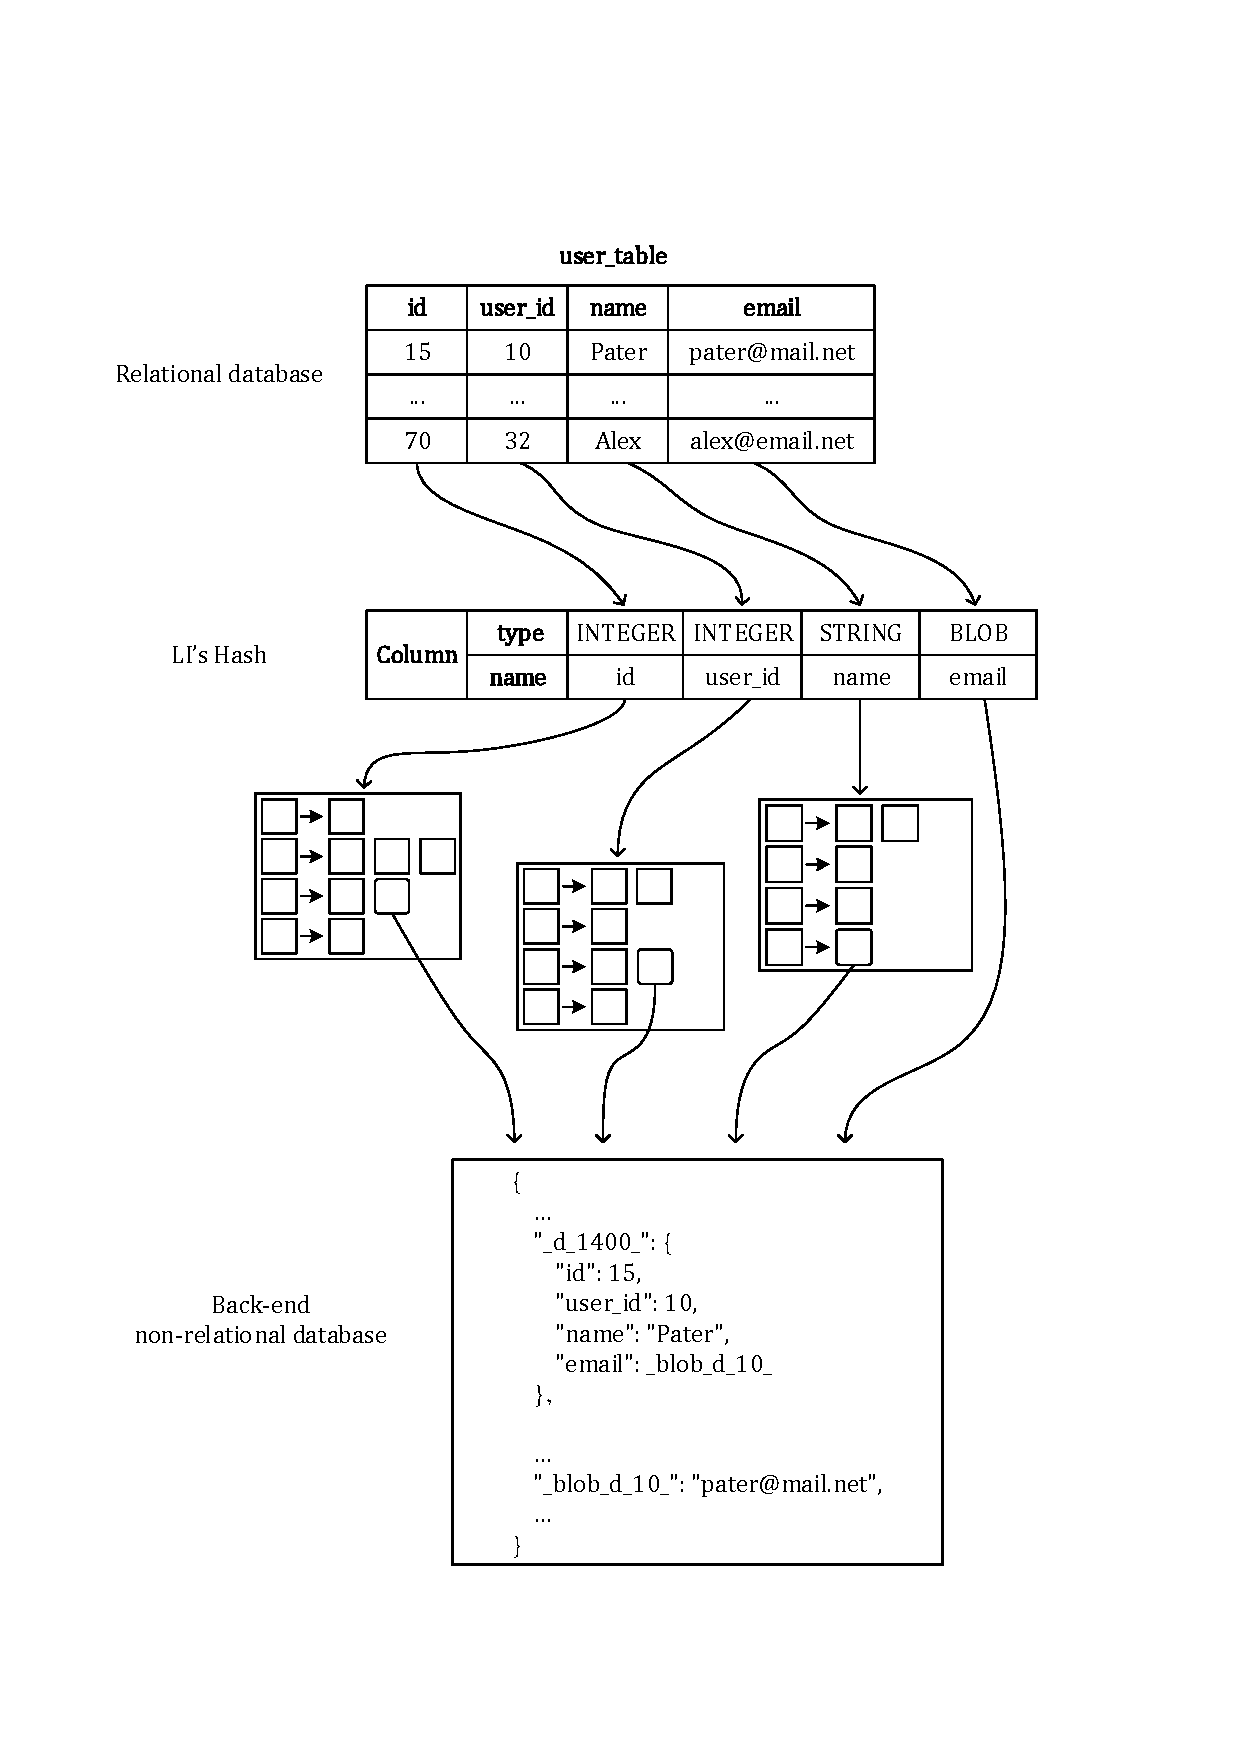
\includegraphics[scale=0.7]{./table-design/pic/design_example_v2.pdf}
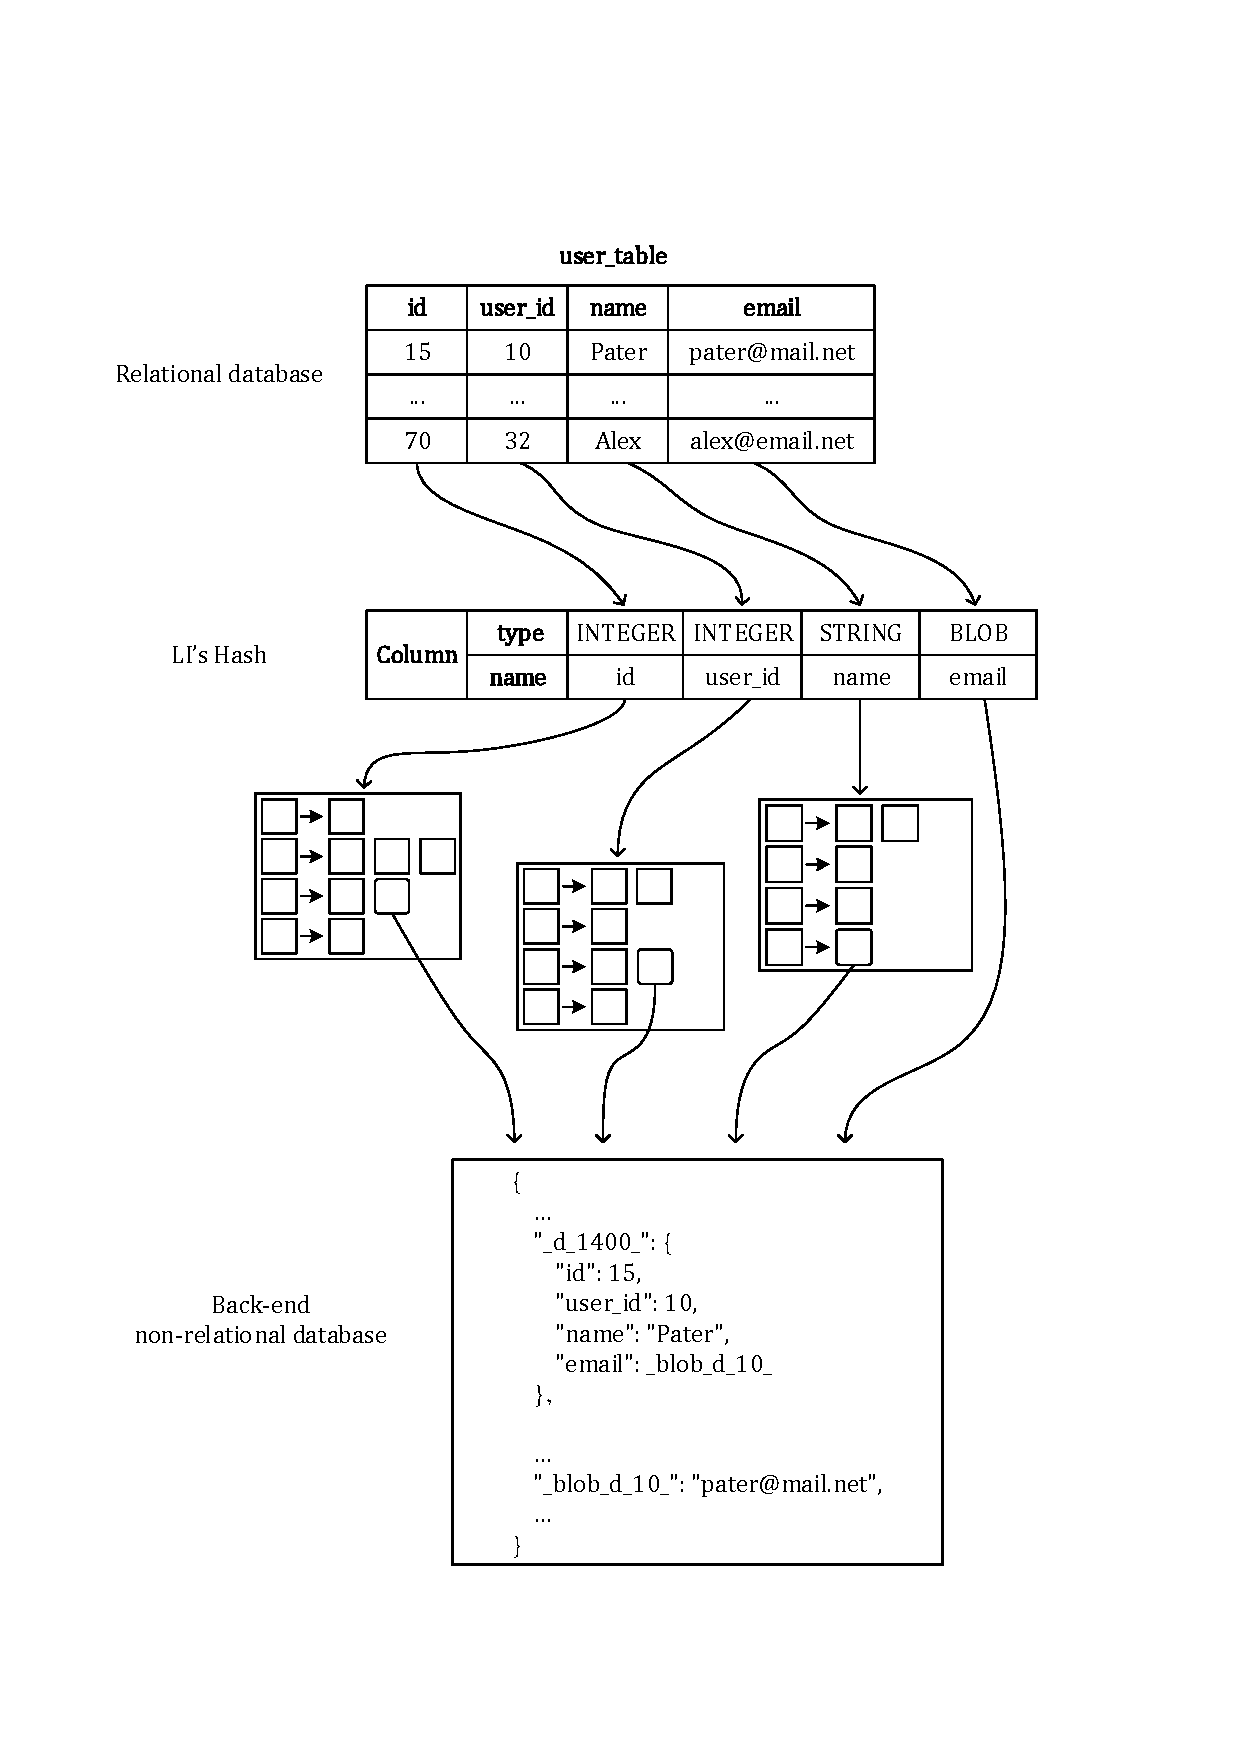
\includegraphics[width=0.6\textwidth]{./table-design/pic/design_example_v2.pdf}
\caption{The view on each layer.}
\label{fig:table_design:example}
\end{figure}

Figure \ref{fig:table_design:example} shows a example of simple membership data-base, the user who using the Li's Hash that will see the view as a normal relational database, but the table is builded by the Li's Hash which do the indexing and store all data into the back-end database just like figure shows.\\

%This is the target that the Li's Hash want to provide for the users.

%table for the user, from the relational databases design \cite{web:mysql:sql-syntax-identifiers,web:sqlite:limits,web:postgresql:sql-syntax-identifiers} which seem normally to set the maximum length of table and column name as 63~64 or no limited. So the maximum length should be 255 for the names which should enough for many user, also plus the length of database's name (for application that multiuser using a single backend database) and the key's length (255 as the other non-relational databases), it should be at least 1000,

\clearpage

% ------------------------------------------------
% End of page
% ------------------------------------------------


% Performance section
%% ------------------------------------------------
% Page start
% ------------------------------------------------
\chapter{Performance Evaluation}
\label{chapter:performance-evaluation}

\baselineskip=26pt
\thispagestyle{empty}
% ------------------------------------------------

% Time evaluation section
\subsection{Time evaluation}

% Setup section
\subsubsection{Setup}

To measure the performance of Li's Hash by measuring the time of each data type (except BLOB) and operation and compare with SQLite \cite{web:sqlite:home-page}, MariaDB \cite{web:mariadb:home-page} and PostgreSQL \cite{web:postgresql:home-page} by using single table in memory to remove any possible I/O delay.\\

There is no SQL parser for Li's Hash which may this test un-fair, but a SQL parser can't too slow because it is one of core part for a SQL database. We observe the timing of SQLite and it take < 0.001 ms per SQL on our platform. So it seem that the time is too small that can be ignore.\\

Also, because normally the real hash table will use the index as a pointer, but the problem is that kind of hash table need to use a static array, but a dynamic hash table that even the std::map in standard C++ library, it still need to use the $\log(n)$ like the other B+ tree does.\\

So if still use these kind library as our back-end storage to do the testing which will not see the improvement of our design, so that we implemented our own back-end storage based on Radix tree \cite{web:wiki:radix-tree} and it work similar as the design of the Linux kernel does \cite{web:linux-kernel:radix-tree}.\\

%\begin{figure}[h]
%\centering
%\includegraphics[scale=0.5]{./performance/pic/a.png}
%\caption{The Radix tree design.}
%\label{fig:performance:}
%\end{figure}

%Figure \cite{fig:performance:} is our design look like, we hash the key become a number (Same as the ring design in Dynamo \cite{paper:amazon-dynamo-1}), next convert the number into byte array which that the index will become its' depth and the value of the byte will be as its' index number for moving to the downward, until found the leaf which is the data storage.\\

%Collision is very easy happen in hash function, we can do two way to slove it in our tree design:

%\begin{enumerate}

%\item \textbf{Increase the depth of tree}\\
%Increase the byte length of the hash function output, which means incease the depth of tree.

%\item \textbf{Multi-level tree}\\
%Our Radix tree can become a multi-level tree, will mean the leaf can become the root of the next level tree.

%The reason of this design is a single hash function still can cause a very small collision, so if using a tree that build from multi-hash function that should highly decrease the collision probelm.

%\end{enumerate}

% Testing section
\subsection{Testing}

We use the default configure for SQLite base on assume the user is new for it, then he/she will only care the performance in the default, also the default is set by the offical that what they think is the best, so this can be as a baseline of the database.\\

%We use 100,000 rows (keys) for test the performance on our platform. The reason is because we tested up to 500,000 and found out when SQLite enabled the indexing, the average time per SQL seem very static, so testing more rows seem don't prodive any useful information.

% Hardware table

\begin{table}[ht]
\centering
\label{table:performance:testing-platform}
\begin{tabular}{|c|c|}

\hline
\multicolumn{1}{|r|}{CPU:} &
\multicolumn{1}{c|}{Intel Xeon E5-2620} \\

\hline
\multicolumn{1}{|r|}{RAM:} &
\multicolumn{1}{c|}{180 GB} \\

\hline
\multicolumn{1}{|r|}{OS:} &
\multicolumn{1}{c|}{Ubuntu 12.04.4} \\

\hline
\multicolumn{1}{|r|}{Kernel:} &
\multicolumn{1}{c|}{3.11.0-15-generic} \\

\hline
\multicolumn{1}{|r|}{GCC version:} &
\multicolumn{1}{c|}{4.6.3} \\

\hline
\multicolumn{1}{|r|}{SQLite version:} &
\multicolumn{1}{c|}{3.8.1} \\

\hline
\end{tabular}
\end{table}



\clearpage

% ----------------------------------------------------------

\begin{enumerate}


%In this layer, we test the baseline of all databases without using the index, but without index the Li's Hash can't do query as a normal non-relational database. So we only test the performance of the back-end database by only use the basic put(), get() for all data type in Li's Hash. Also only use normal SELECT, INSERT in relational database without enable index.\\

% Database layer section
\item \textbf{Database layer}

In this layer, we test the baseline of both databases without using the index, but without index the Li's Hash can't do query as a normal non-relational data-base. So we only test the performance of the back-end data-base by using the basic \textit{put()}, \textit{get()} for all data type in Li's Hash. Also only use normal SELECT, INSERT in relational database without enable index. We use the code in table \ref{table:performance:database-layer:code-example} to do this test.\\

% Database layer test table 

% Database layer test
\begin{table*}
\centering
\caption{Example code that to test STRING type in \textit{Database layer}}
\label{table:performance:database-layer:code-example}
\begin{tabular}{|c|c|c|}

\hline
\multicolumn{1}{|c|}{} &
\multicolumn{1}{c|}{\textbf{Li's Hash}} &
\multicolumn{1}{c|}{\textbf{Relational database}} \\

\hline
\multicolumn{1}{|c|}{Create table} &
\multicolumn{1}{c|}
{\tabincell{c}{
X \\ (Key-value store don't need table)
}} &
\multicolumn{1}{l|}{CREATE TABLE table(value TEXT) ;} \\

\hline
\multicolumn{1}{|c|}{Insert} &
\multicolumn{1}{l|}{put('key-\textit{i}', 'value-\textit{i}')} &
\multicolumn{1}{l|}{INSERT INTO table('value') VALUES ('value-\textit{i}') ;} \\

\hline
\multicolumn{1}{|c|}{Select} &
\multicolumn{1}{l|}{get('key-\textit{i}')} &
\multicolumn{1}{l|}{SELECT value FROM table LIMIT \textit{i}, 1 ;} \\

\hline
\end{tabular}
\end{table*}



% Database layer result

\begin{figure*}
\centering
%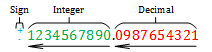
\includegraphics[scale=1.0]{./algorithm/real/pic/design/data_format_v2.png}
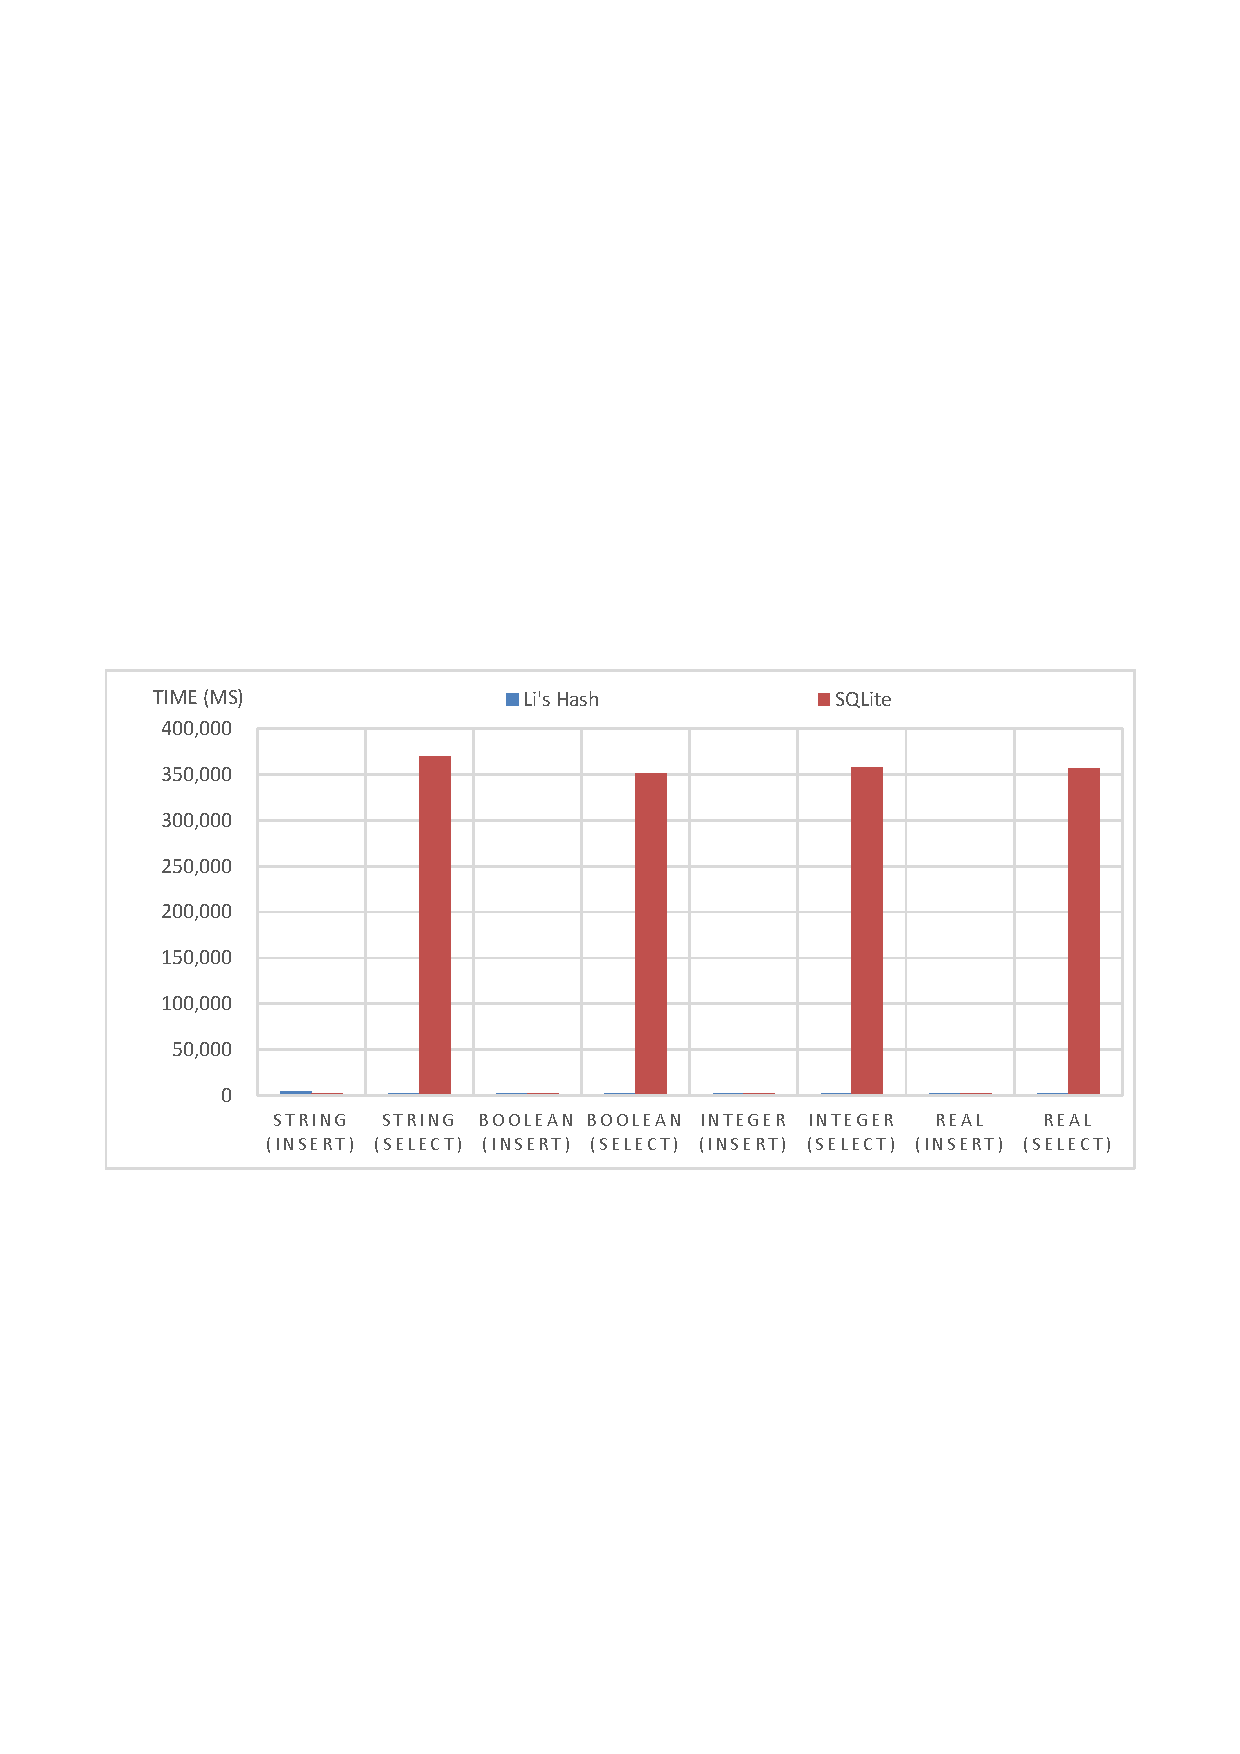
\includegraphics[width=0.8\textwidth]{./performance/result/database-layer/image/100only/full2.pdf}
\caption{Performance on database layer}
\label{fig:performance:result:database-layer}
\end{figure*}



\clearpage

% ----------------------------------------------------------

% Index layer section
\item \textbf{Index layer}

Fellow the test in \textit{Database layer}, but this time we include the index part, remove(), update() for Li's Hash. Also test DELETE, UPDATE with enable the index in relational database which using the code of table \ref{table:performance:index-layer:code-example}.\\

% Index layer test table 

% Index layer test
\begin{table*}[width=\textwidth]
\centering
\caption{Example code that to test STRING type in \textit{Index layer}}
\label{table:performance:index-layer:code-example}
\begin{tabular}{|c|c|c|}

\hline
\multicolumn{1}{|c|}{} &
\multicolumn{1}{c|}{\textbf{Li's Hash}} &
\multicolumn{1}{c|}{\textbf{Relational database}} \\

\hline
\multicolumn{1}{|c|}{Create table} &
\multicolumn{1}{l|}
{\tabincell{l}{
create\_table('table', 'value', STRING\_TYPE)
}} &
\multicolumn{1}{l|}
{\tabincell{l}{
CREATE TABLE table(id INT, value TEXT) ; \\
CREATE INDEX idx\_value ON table (value) ;
}} \\

\hline
\multicolumn{1}{|c|}{Insert} &
\multicolumn{1}{l|}
{\tabincell{l}{
insert('table', 'value-\textit{i}')
}} &
\multicolumn{1}{l|}
{\tabincell{l}{
INSERT INTO table('value') VALUES ('value-\textit{i}') ;
}} \\

\hline
\multicolumn{1}{|c|}{Select} &
\multicolumn{1}{l|}
{\tabincell{l}{
select('table', 'value', 'value-\textit{i}')
}} &
\multicolumn{1}{l|}
{\tabincell{l}{
SELECT value FROM table \\
WHERE value = 'value-\textit{i}' ;
}} \\

\hline
\multicolumn{1}{|c|}{Update} &
\multicolumn{1}{l|}
{\tabincell{l}{
update('table', 'value', 'value-\textit{i}', 'value-\textit{i}-')
}} &
\multicolumn{1}{l|}
{\tabincell{l}{
UPDATE table SET 'value' = 'value-\textit{i}-' \\
WHERE value = 'value-\textit{i}' ;
}} \\

\hline
\multicolumn{1}{|c|}{Remove} &
\multicolumn{1}{l|}
{\tabincell{l}{
remove('table', 'value', 'value-\textit{i}-')
}} &
\multicolumn{1}{l|}
{\tabincell{l}{
DELETE FROM table WHERE value = 'value-\textit{i}' ;
}} \\

\hline
\end{tabular}
\end{table*}



% Index layer result 

\begin{figure*}
        \centering

        \begin{subfigure}[b]{0.4\textwidth}
                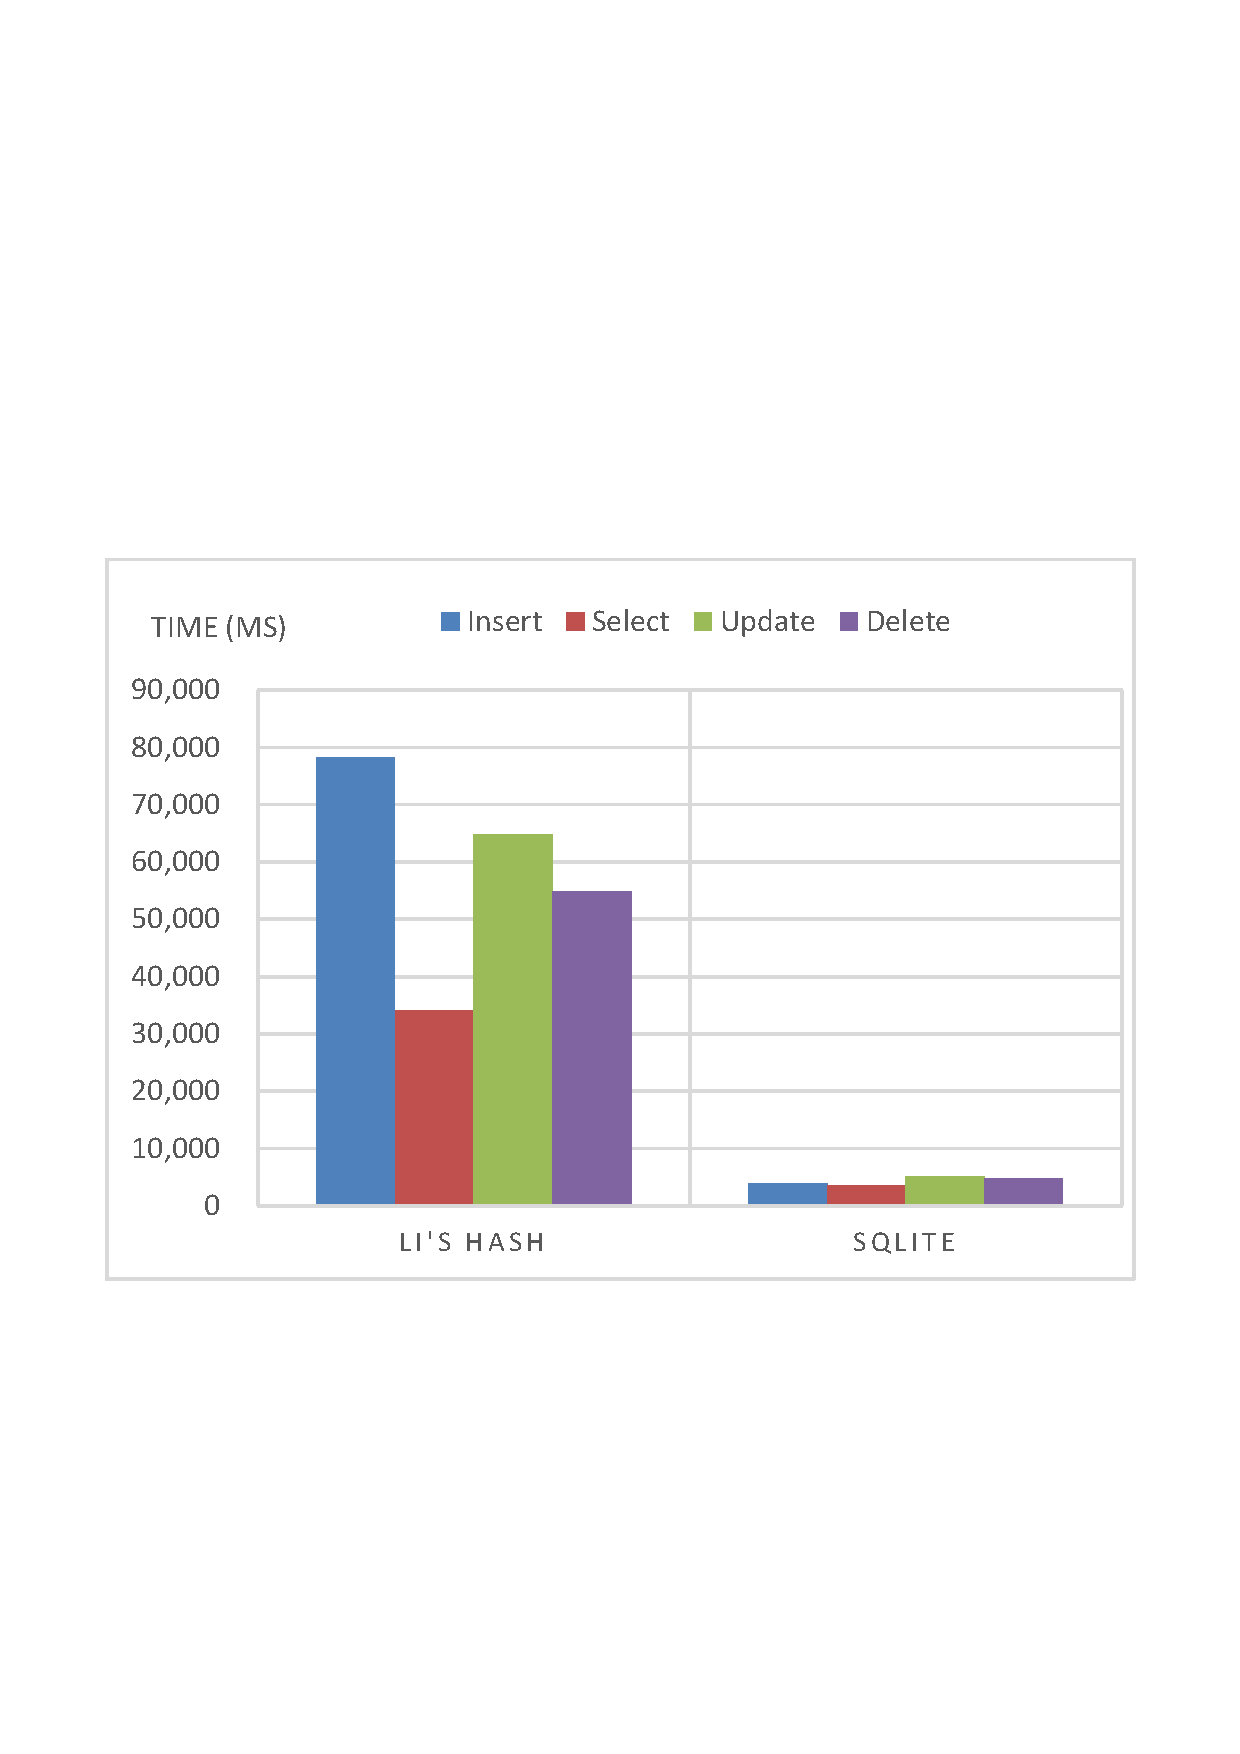
\includegraphics[width=\textwidth]{./performance/result/index-layer/image/100only/string1.pdf}
                \caption{STRING type}
                \label{fig:performance:result:index-layer:insert:boolean}
        \end{subfigure}%
        ~ %add desired spacing between images, e. g. ~, \quad, \qquad etc.
          %(or a blank line to force the subfigure onto a new line)
        \begin{subfigure}[b]{0.4\textwidth}
                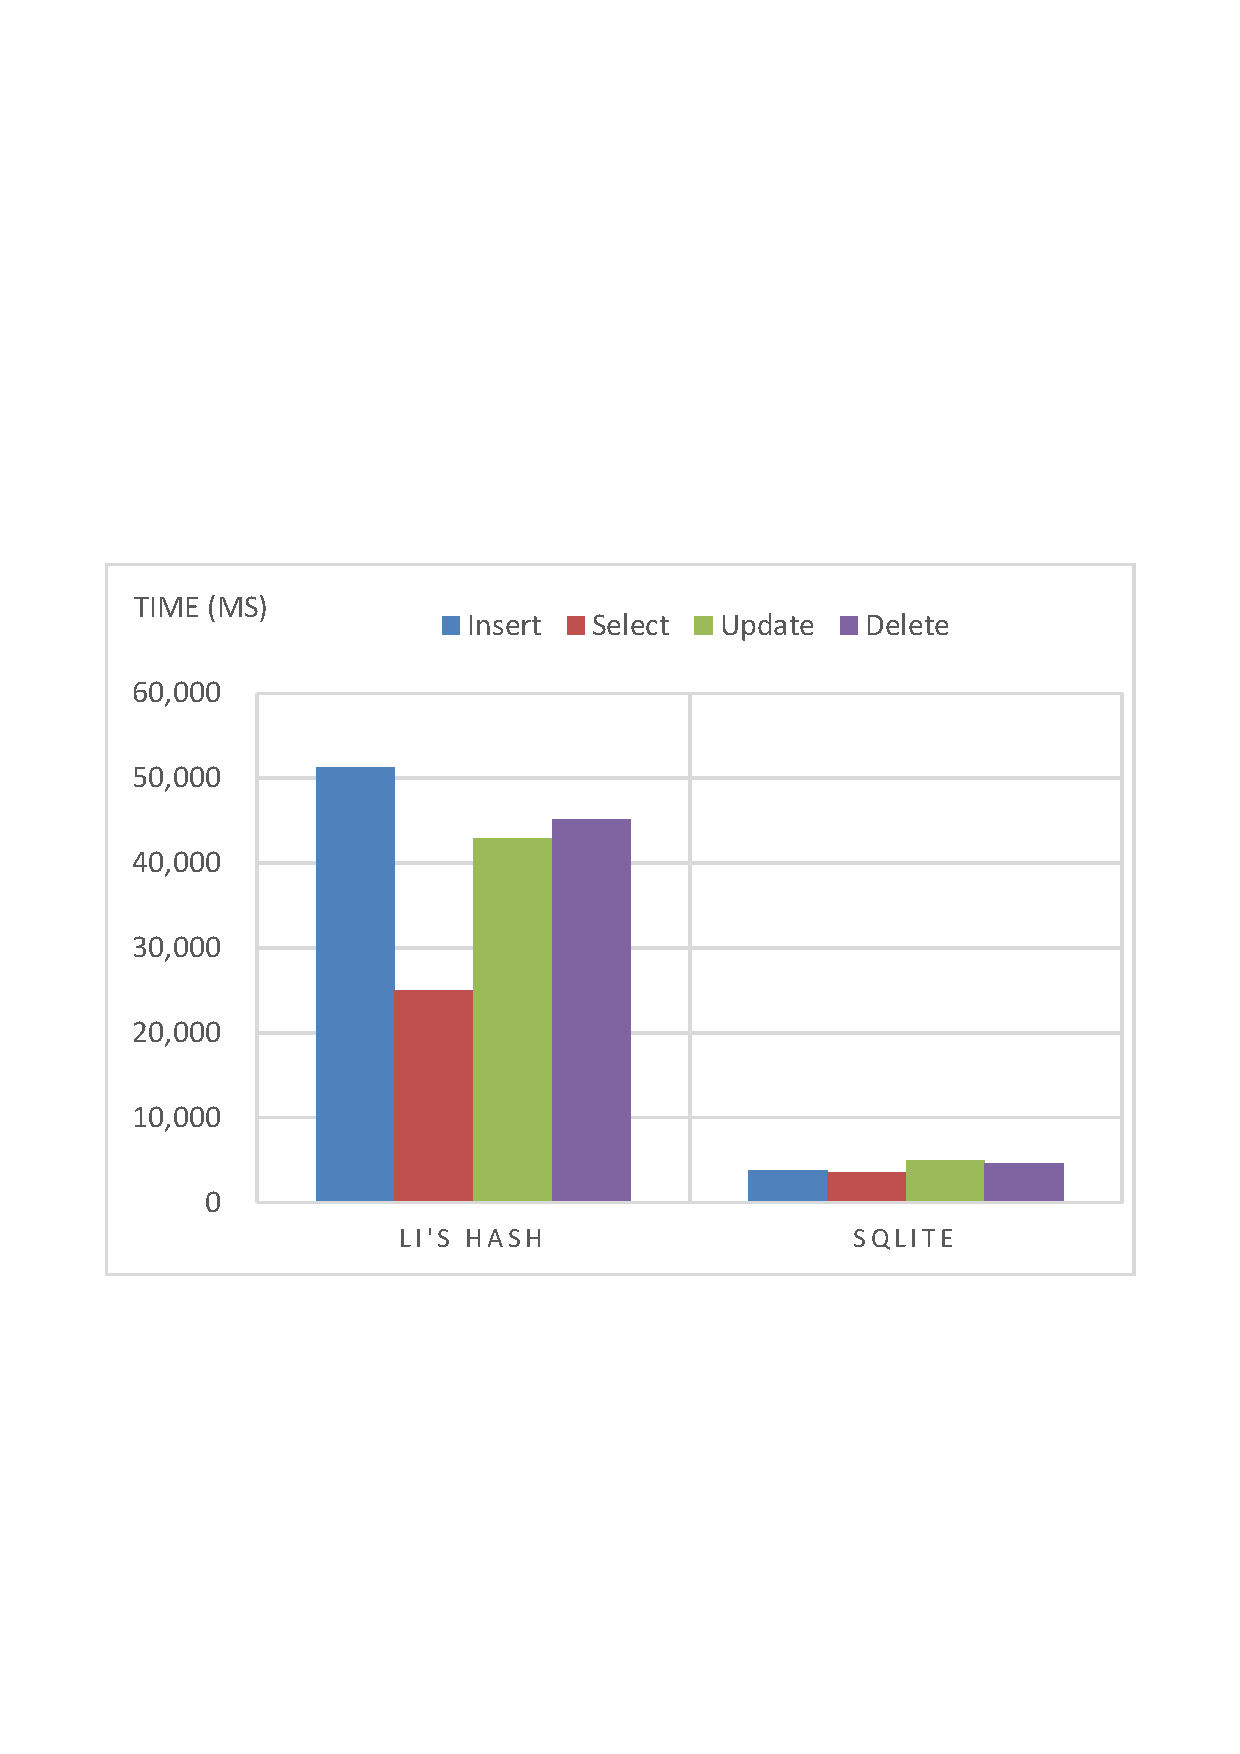
\includegraphics[width=\textwidth]{./performance/result/index-layer/image/100only/boolean1.pdf}
                \caption{BOOLEAN type}
                \label{fig:performance:result:index-layer:insert:int}
        \end{subfigure}

        \begin{subfigure}[b]{0.4\textwidth}
                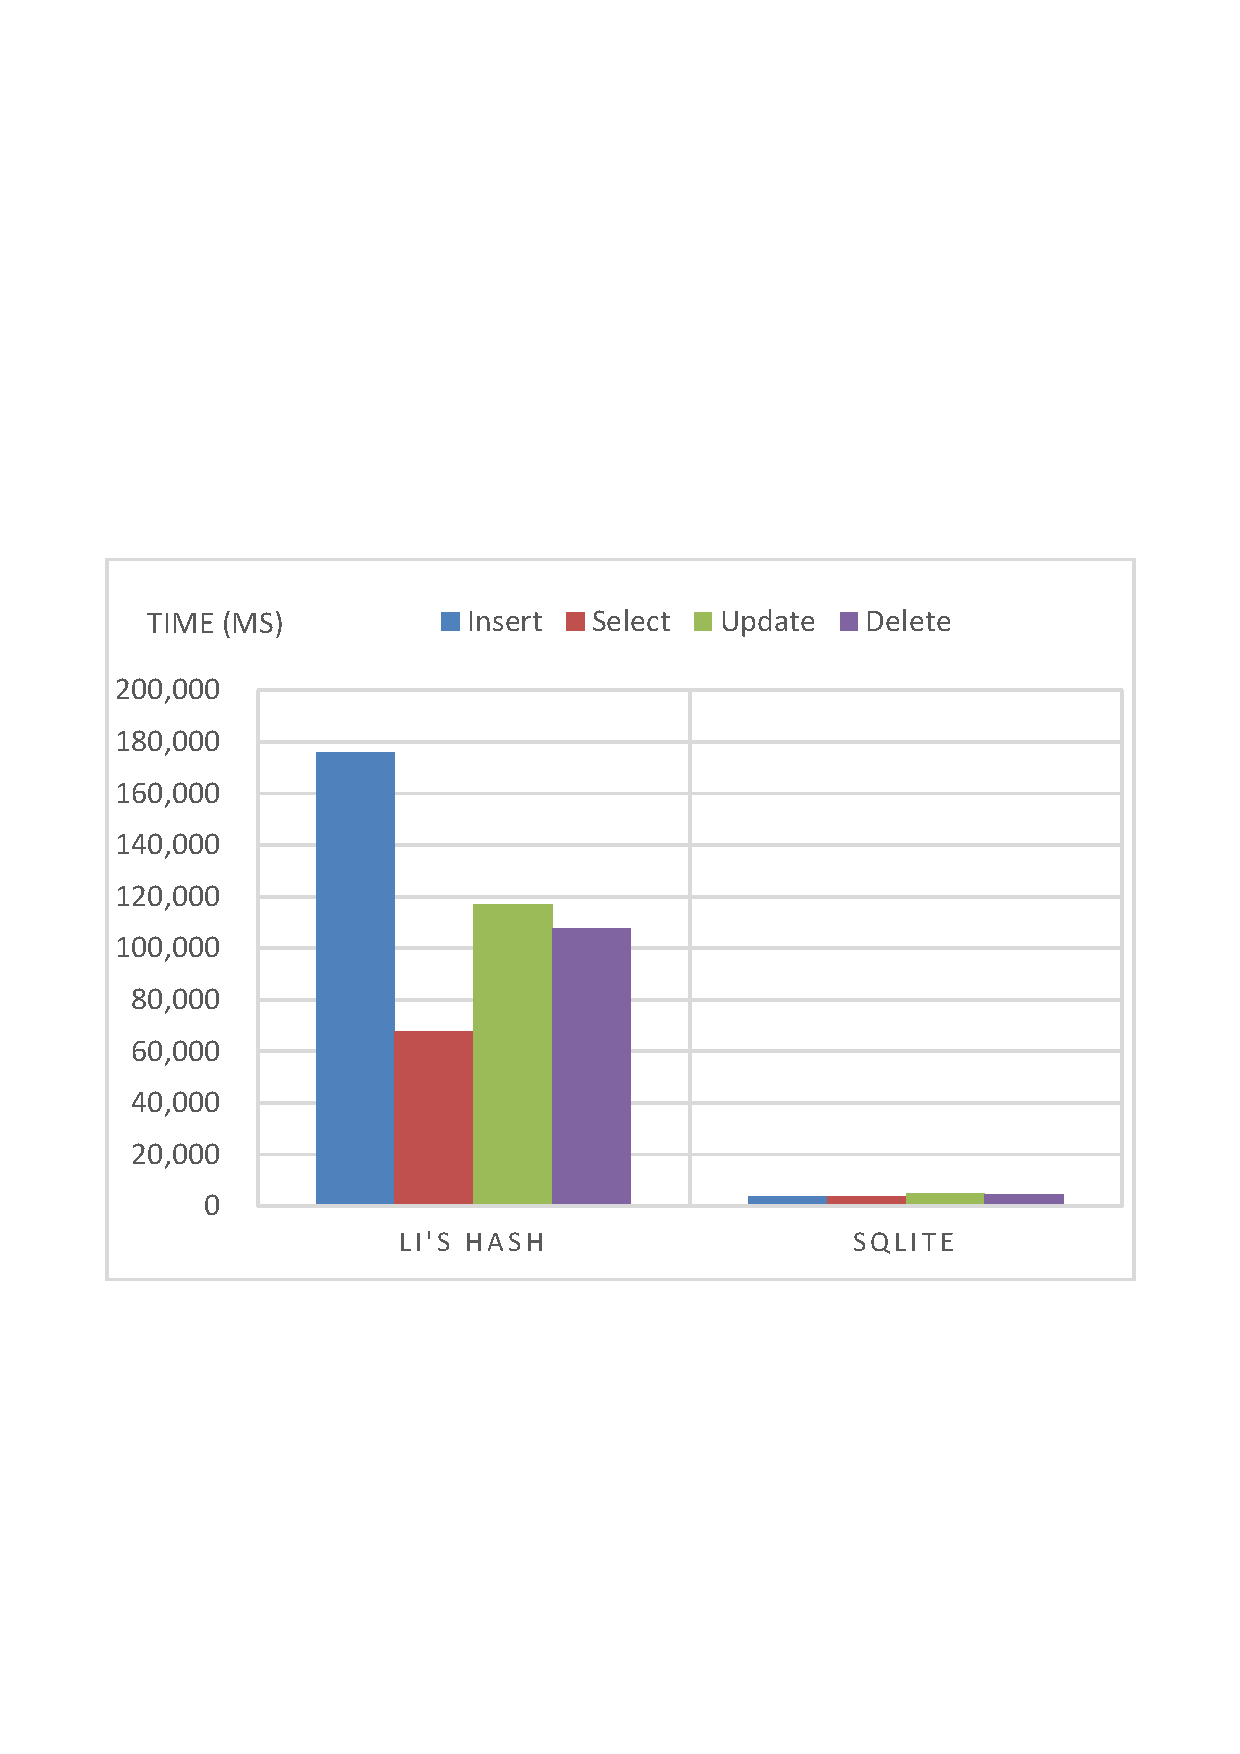
\includegraphics[width=\textwidth]{./performance/result/index-layer/image/100only/integer1.pdf}
                \caption{INTEGER type}
                \label{fig:performance:result:index-layer:insert:real}
        \end{subfigure}
        ~ %add desired spacing between images, e. g. ~, \quad, \qquad etc.
          %(or a blank line to force the subfigure onto a new line)
        \begin{subfigure}[b]{0.4\textwidth}
                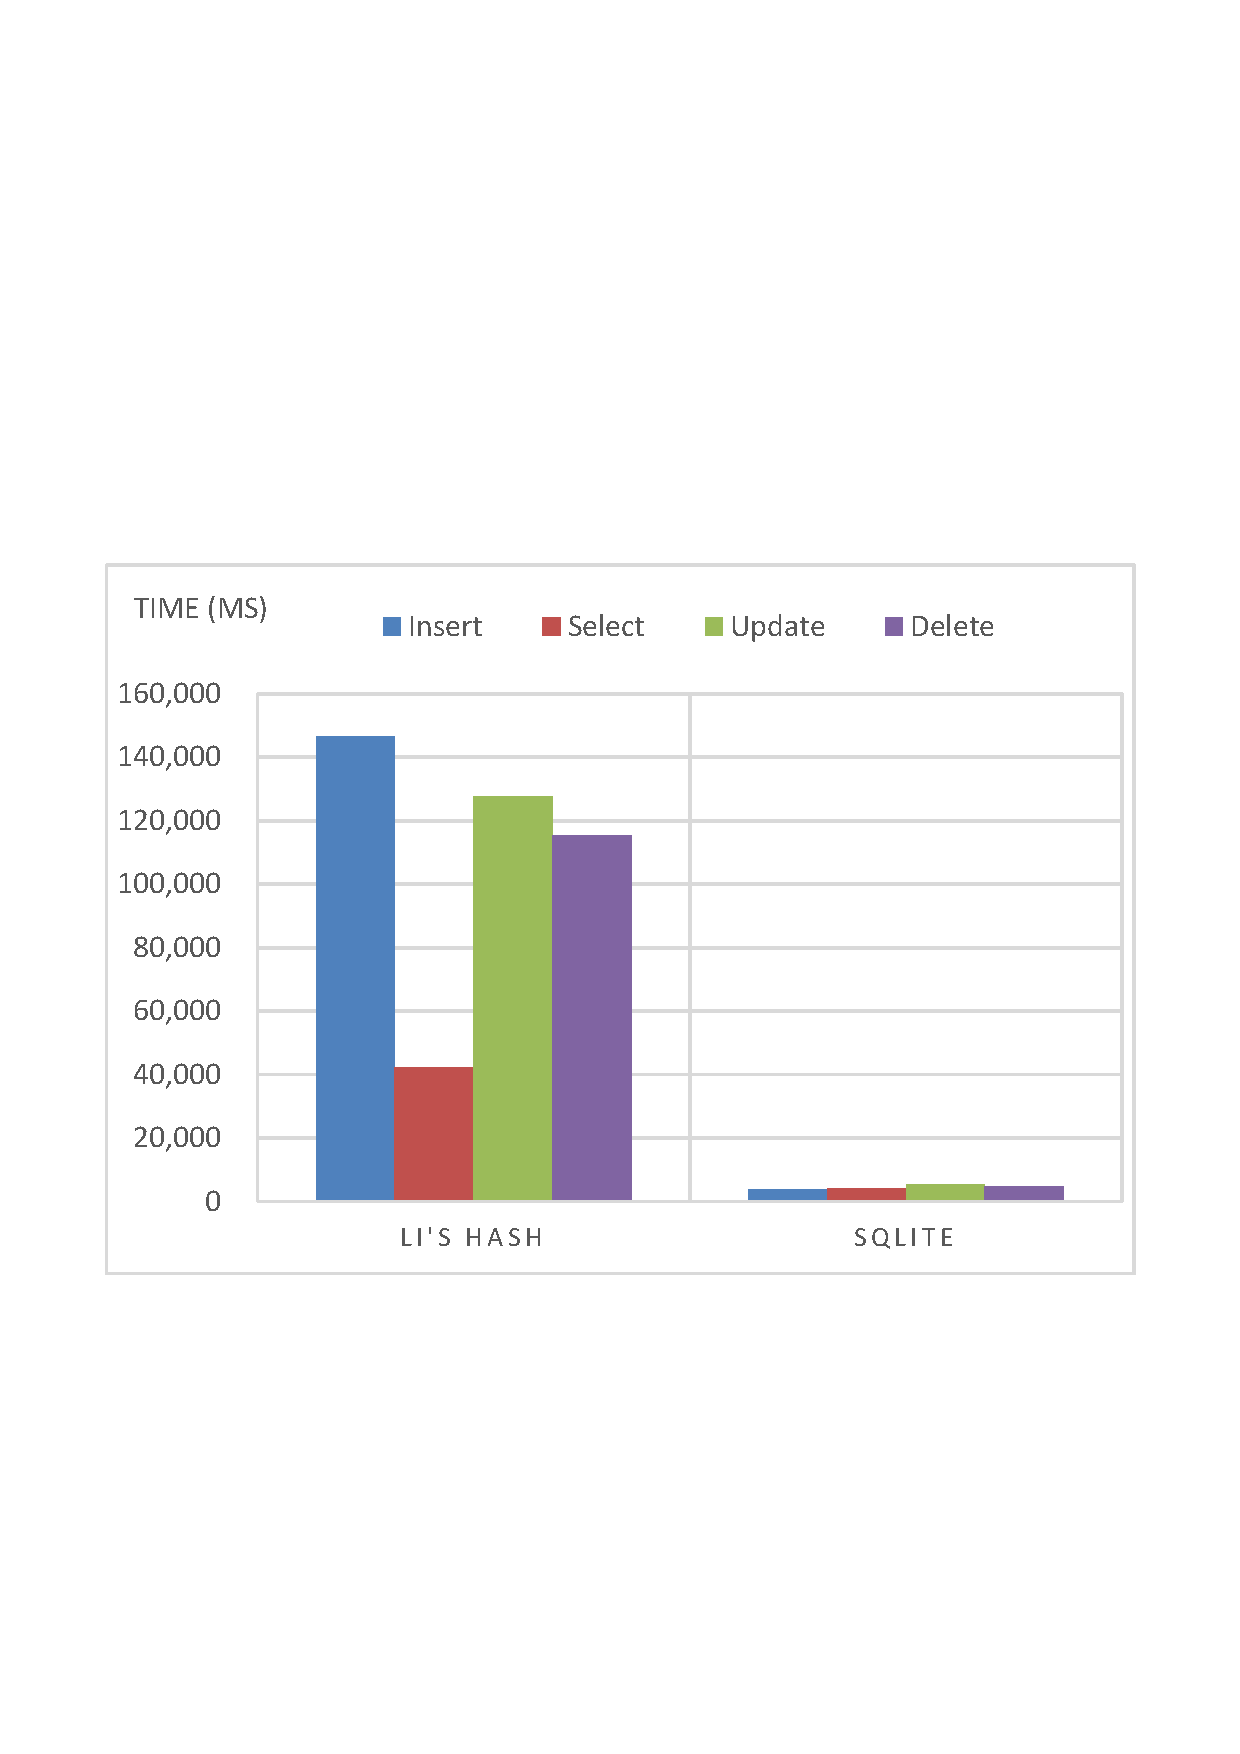
\includegraphics[width=\textwidth]{./performance/result/index-layer/image/100only/real1.pdf}
                \caption{REAL type}
                \label{fig:performance:result:index-layer:insert:string}
        \end{subfigure}

        \caption{Performance on index layer}
        \label{fig:performance:result:index-layer}
\end{figure*}



\clearpage

% ----------------------------------------------------------

% Joining section
\item \textbf{Joining operation}

Joining always is one of the bottleneck of the relational database, but it is just a intersection operation for Li's Hash. So in this test, we let them to do the a mutli-table joining.\\

\begin{figure}[h]
\centering
\includegraphics[scale=0.8]{./performance/pic/multi-table_v1.png}
\caption{A example of mutli-table joining.}
\label{fig:performance:multi-table}
\end{figure}

The mutli-table is look like figure \ref{fig:performance:multi-table}, this example is a very sample joining in Human thought, but it still can be a over-hand of the relational database. This example is just search the value by joining many table in the middle, the starting point is the column "Key" in Table 1 and finish is the "Value" column in the Table N, between them is a ton of the pointer which is use for pointing to the next pointer in the next table, so that when search the value which will need to joining these tables and pointer to get the correct value.\\

So this should need to use complex SQL and need times to do that, which will get our a result that the Li's Hash can do the  joining operation and a better time.\\

\clearpage

% ----------------------------------------------------------

\end{enumerate}

% Result section
\subsection{Result}

Figure \ref{fig:performance:result:database-layer} and \ref{fig:performance:result:index-layer} are shows that it is faster after enabled the indexing in SQLite, also Li's Hash become slower because the indexing rather directly using the \textit{put()} or \textit{get()} that because it need to build the index table.\\

In this testing, the main point is not to test how good as the Li's Hash compare to a well-known embedded relational database, but to test it is workable or not, so our will focus on the improvement and the application extension (such as graph database, base on the same table design) to provide different angle and usage.\\

\clearpage

% ------------------------------------------------
% End of page
% ------------------------------------------------


% Requirement section
%% ------------------------------------------------
% Page start
% ------------------------------------------------
\chapter{Requirement}
\label{chapter:requirement}

\baselineskip=26pt
\thispagestyle{empty}
% ------------------------------------------------

Although Li's Hash is design for all key-value stores, but still Li's Hash is need to work basic on some requirements:

\begin{enumerate}

\item \textbf{No limited key's length}\\
For some key-value stores has limited the key length such as only 255 long (like ArangoDB \cite{web:arangodb:comparison}), this will limited the upper application's key design, this is not a good thing that limit an application what it can do only.\\

Like LevelDB \cite{web:leveldb:home-page} and Voldemort \cite{web:voldemort:any-limit-store-key} which keep the keys and values as byte arrays which means it has no limited the length.

\item \textbf{A suitable value's length}\\
The value's length of the back-end database can't too short, at least 4096 bytes long. Li's Hash design the length of value which default set the maximum size as 4096 bytes, if input value is longer than 4096 bytes, it will cut it into multi-key for storing it.\\

 This value should be not set too large such as 128 MB, which is because if the size is too large that every searching is need to allocate the same amount of memory to read the data in value, unless the hardware have a huge memory space, otherwise in the multithread environment it can out of memory. Also reading a huge data from disk will increase the I/O times.

\item \textbf{Unlimited key's amount}\\
Limited the amount of key is as same as limited the row in table in the relational database, normally this should not happed but it happened in the storage engine of Apache Cassandra which set the maximum number of cells (rows x columns) in a single partition (table) is 2 billion \cite{web:cassandra:limitations}.\\

Therefore if we use key-value pair (rows x 1 column) to think it, it still got 2 billion keys on it. It may seem very enough to many application, but the problem is this will force some application which generate more than 2 billion keys per day or per hour (such as finance information, log data, astronomy data, etc.) need to modify their source code to fit into the database, although there is many way to modify it, but it still increased the programmer's work, and this is one of the wish that Li's Hash want to solve.

\end{enumerate}

\clearpage

% ------------------------------------------------
% End of page
% ------------------------------------------------


% Conclusion and future work section
%% ------------------------------------------------
% Page start
% ------------------------------------------------
\chapter{Conclusion}
\label{chapter:conclusion}

\baselineskip=26pt
\thispagestyle{empty}
% ------------------------------------------------

In big data, the meaning of owning one petabyte or ten petabyte are the same --- meaningless. The true is hiding inside the data, this means how fast can the data retrieval from database and process it to become an information we need that is the major question in this field, and normally the bottleneck is the query operation that between the database \cite{paper:nodb} and the program.\\

So this paper is try to propose Li's Hash (an indexing algorithm) to provide query mechanism on key-value database, the non-relational database which the performance is more suitable on big data area rather than relational database. Li's Hash is to help people use the same concept in relational database but using non-relational database as the back-end.\\

Li's Hash is try to replace some of the work which original need done by MapReduce, because the result can searching on single server, and don't need to write the code of MapReduce or install the platform of MapReduce. So that this can decrease the development cost, lower the conditions for programmer to start writing the program, also accelerate the speed of development.\\

Also because the design, that is using modularized design which can swappable the back-end database, so it is suitable for all key-value stores. Such as Project Voldemort \cite{web:voldemort:home-page} which develop by LinkedIn, or the LevelDB from Google \cite{web:wiki:leveldb}, they do not limits too much to key-value, so that both of them are very suitable as the back-end of Li's Hash.\\

Alough the testing is not so well, but the main point of this paper is not to test how good as the Li's Hash compare to a well-known embedded relational database, but to test it that is workable or not.\\

%\clearpage

% ------------------------------------------------
% End of page
% ------------------------------------------------


% Conclusion and future work section
%% ------------------------------------------------
% Page start
% ------------------------------------------------
\chapter{Future work}
\label{chapter:future-work}

\baselineskip=26pt
\thispagestyle{empty}
% ------------------------------------------------

The next step of Li's Hash is focus on the improvement and the application extension (such as graph database, base on the same table design) to provide different angle and usage.\\

Later on, by adding the SQL parser into the library for handle SQL as the input, which should let the people more comfortable to use it like the normally SQL database. Also provide some more feature for the library is needed, such as multi-table joining operation in SQL, graph database (like Neo4j\cite{web:neo4j:home-page}, by using different back-end database rather than a fixed storage engine), decision tree, similarity (like Lucene \cite{web:wiki:lucene}), etc. These feature are very basic and common that should become very useful in many field, such as information retrieval and data mining.\\

%\clearpage

% ------------------------------------------------
% End of page
% ------------------------------------------------


% ------------------------------------------------

% 參考文獻 References

% ----------------------------------------------------------------------------
%                                 References
%                                   參考文獻
% ----------------------------------------------------------------------------

% Page start
\newpage
\phantomsection

% Add to "Table of Contents"
%\addcontentsline{toc}{chapter}{References}

% Change the title of bibliography
%\renewcommand\bibname{\centerline{\Large References}}

% ------------------------------------------------

\bibliographystyle{abbrv}
\bibliography{./example/references/paper,./example/references/msic}

% ------------------------------------------------
% End of page
% ------------------------------------------------


% ------------------------------------------------

% 附錄 Appendix
% ------------------------------------------------
\StartAppendix
% ------------------------------------------------

% ------------------------------------------------
% Page start
\newpage
\phantomsection
% ------------------------------------------------

\chapter{可使用這模版的系所}
\label{appendix:acceptable-dept}

這邊列出一些\textbf{應該可使用}或\textbf{不可使用}這模版的系所名字, 這表可能會有不正確, 所以還是先問系辦確定會比較好.\\

因為這名單都是靠網路上能找多少而得出的結果, 而如果沒有分類的話, 很高機會是使用圖書館的要求. \\

而如果這表名單中沒有顯示你的系所, 但你已經\textbf{知道}是否能使用, 請告知以供更新.

\clearpage

\section{應該可使用}

    可使用的原因幾乎都是系所自己沒有特殊要求, 所以直接使用圖書館的要求, 而本模版就是跟隨圖書館所定下的要求來設計.

    \begin{table*}[pht]
    \centering
    \caption{應該可使用的系所}
    \label{table:acceptable-dept:acceptable}
    \begin{tabular}{|c|c|}

    \hline
    \multicolumn{1}{|c|}{資訊工程學系} &
    \multicolumn{1}{c|}{Department of Computer Science and Information Engineering} \\

    \hline
    \end{tabular}
    \end{table*}

\section{應該不可使用}

    不可使用的原因是系所自己已經有提供一份樣版出來, 而那份樣版的要求有沒有跟本模版一樣設計, 這個就不作詳細分析. 故如果已經有樣版, 那我就會把它們分類成\textit{無法使用這本模版}比較好, 但如果分類錯誤, 請告知.

    \begin{table*}[pht]
    \centering
    \caption{應該不可使用的系所}
    \label{table:acceptable-dept:unacceptable}
        \begin{tabular}{|c|c|c|}

        \hline
        \multicolumn{1}{|c|}{生物科技研究所} &
        \multicolumn{1}{c|}{Institute of Biotechnology} &
        \multicolumn{1}{c|}{\href{www.biotech.ncku.edu.tw/files/archive/331_4b79187a.doc}{樣版URL}} \\

        \hline
        \multicolumn{1}{|c|}{體育健康與休閒研究所} &
        \multicolumn{1}{c|}{
            \tabincell{l}{
            Institute of Physical Education,\\
            Health and Leisure Studies
            }
        } &
        \multicolumn{1}{c|}{\href{www.ncku.edu.tw/~deprb/docs/Thesis\%20Regulation\%20.doc}{樣版URL}} \\

        \hline
        \end{tabular}
    \end{table*}

% ------------------------------------------------
% End of page
% ------------------------------------------------

%% ------------------------------------------------
\StartChapter{繳交流程說明}
% ------------------------------------------------

這部份資料來源是使用'電子學位論文服務'提供的'電子學位論文服務流程說明圖'\RefBib{web:lib:submit-flow}和'繳交論文全文電子檔案說明'\RefBib{web:lib:submit-file}.\\

\setboolean{@twoside}{false}
\includepdf[pages=-]{./example/appendix/pdf/2012050004-a.pdf}
\includepdf[pages=-]{./example/appendix/pdf/2012050006-a.pdf}

% ------------------------------------------------
\EndChapter
% ------------------------------------------------

% ------------------------------------------------
% Page start
\newpage
\phantomsection
% ------------------------------------------------

\chapter{各系所博碩士撰寫論文須知}
\label{appendix:thesis-spec}

\section{介紹}
這部份資料來源是使用'電機工程系辦網頁'中的'論文撰寫須知.pdf'(\url{http://office.ee.ncku.edu.tw/uploads/%E8%AB%96%E6%96%87%E6%92%B0%E5%AF%AB%E9%A0%88%E7%9F%A5.pdf}).\\

但由於原檔案沒法顯示, 故需要另重新儲存成一個新的出來. 使用學校的Adobe Acrobat XI試驗, 發現要使用'儲存為其他->可存檔PDF (PDF/A)'才能顯示出來.\\

\begin{figure}[h]
\centering
\includegraphics[scale=0.3]{./example/appendix/pic/save_pdf.png}
\caption{在Adobe Acrobat另存新版本}
\label{fig:appendix:save_pdf}
\end{figure}

檔案位置:\\
新: 'example/appendix/pdf/thesis-spec.pdf'\\
原: 'example/appendix/pdf/論文撰寫須知.pdf'\\

\setboolean{@twoside}{false}
\includepdf[pages=-]{./example/appendix/pdf/thesis-spec.pdf}

% ------------------------------------------------
% End of page
% ------------------------------------------------

%% ------------------------------------------------
\StartChapter{電子論文上傳前檢查事項}{appendix:e-paper_upload}
% ------------------------------------------------

\section{介紹}
這部份資料來源是使用'成功大學電子學位論文服務'中的'電子論文上傳前檢查事項'的'2012090001.pdf'.\\

同樣原檔案沒法顯示, 故需要進行另儲存.\\

檔案位置:\\
新: 'example/appendix/pdf/2012090001-a.pdf'\\
原: 'example/appendix/pdf/2012090001.pdf'\\

\setboolean{@twoside}{false}
\includepdf[pages=-]{./example/appendix/pdf/2012090001-a.pdf}

% ------------------------------------------------
\EndChapter
% ------------------------------------------------

%% ------------------------------------------------
\StartChapter{學位論文上傳說明}{appendix:e-paper_upload_ppt}
% ------------------------------------------------

這部份資料來源是使用'電子學位論文服務'提供的 '2015論文提交說明簡報檔'\RefBib{web:lib:2015-submit-ppt} 修改而成的, 只抽出使用本模版後, 還要做什麼的行為.\\

\setboolean{@twoside}{false}
\includepdf[pages=-]{./example/appendix/pdf/2012050003-short-a}

% ------------------------------------------------
\EndChapter
% ------------------------------------------------


%% ------------------------------------------------
\StartChapter{口試注意事項}
% ------------------------------------------------

這部份資料來源是使用本系資訊工程研究所系辦所提供的資料, 雖然內容主要針對本系, 但某些內容都是適合非本系的同學們.

\setboolean{@twoside}{false}
\includepdf[pages=-]{./example/appendix/pdf/oral-1040616-a.pdf}

% ------------------------------------------------
\EndChapter
% ------------------------------------------------

%% ------------------------------------------------
\StartChapter{常見問題Q\&A}{appendix:faq}
% ------------------------------------------------

\StartSection{介紹}
這部份資料來源是使用'電子學位論文服務'提供的'FAQ'\RefBib{web:lib:ETDS-QA}, 用來補充其他Appendix沒提到的一些情報.\\

\setboolean{@twoside}{false}
\includepdf[pages=-]{./example/appendix/pdf/2012050009-a.pdf}

% ------------------------------------------------
\EndChapter
% ------------------------------------------------

%% ------------------------------------------------
\StartChapter{LaTex Symbol寫法}{appendix:unicode-symbols}
% ------------------------------------------------

這部份資料來源是xeCJK的v3.3.4(2016/02/10)版本中提供的50頁有關所有Symbol的寫法, 極度值得同學們閱讀或在這邊找你所需的Symbols.\\

內容的說明方式為:\\
Symbol: 符號所顯示的樣子\\
USV: 以Unicode方式所代表的這個符號, 例如 `(' 的Unicode寫法為U+0028.\\
Description: 是這符號的名字.\\
Macro(s): 是LaTex使用這符號的寫法.\\

\textbf{P.S: }因為符號數量多, 沒法100\%保證全能使用.

\setboolean{@twoside}{false}
\includepdf[pages=-]{./example/appendix/pdf/xunicode-symbols.pdf}

% ------------------------------------------------
\EndChapter
% ------------------------------------------------


% ------------------------------------------------
\EndAppendix
% ------------------------------------------------


% ------------------------------------------------
